\documentclass[12pt, twoside, openright]{report}
\usepackage[a4paper,left=25mm,right=25mm,top=25mm,bottom=25mm]{geometry}
\usepackage{graphicx} % Required for inserting images
\usepackage{natbib}
\let\OLDthebibliography\thebibliography
\renewcommand\thebibliography[1]{
  \OLDthebibliography{#1}
  \setlength{\parskip}{0pt}
  \setlength{\itemsep}{0pt plus 0.3ex}
}

\usepackage{fancyhdr}
\usepackage{setspace}
\usepackage{glossaries}
\usepackage[utf8]{inputenc}
\usepackage{aas_macros}
\usepackage{relsize}
\usepackage{subcaption}
\usepackage{multirow}
\usepackage{rotating}
\usepackage{amssymb}
\usepackage{bookmark}
\usepackage[cleardoublepage=plain]{scrextend}

\onehalfspacing

\usepackage[skip=2pt, indent=20pt]{parskip}

\renewcommand{\footnoterule}{%
  \kern -3pt
  \hrule width \textwidth height 1pt
  \kern 2pt
}
\interfootnotelinepenalty=10000

\fancyhead[LO]{\nouppercase{\leftmark}}
\fancyhead[RO]{\nouppercase{\rightmark}}
\fancyhead[LE]{\nouppercase{Luke R. Holden}}
\fancyhead[RE]{\nouppercase{Precise diagnostics of AGN-driven outflows}}

\usepackage{xcolor}
% \definecolor{lrhblue}{HTML}{009DFF}
\definecolor{lrhdarkblue}{HTML}{004f80}
% \definecolor{lrhorange}{HTML}{f4a250}
\definecolor{lrhdarkorange}{HTML}{a8590b}

\usepackage{hyperref}
\hypersetup{
    colorlinks = True,
    linkcolor=lrhdarkorange,
    citecolor=lrhdarkblue,
    urlcolor=lrhdarkorange,
}

\usepackage{tocloft}    %%%%
\cftsetrmarg{5em}       %%%%

\emergencystretch 3em

\widowpenalty10000
\clubpenalty10000

\begin{document}

\pagenumbering{roman}

\pagestyle{empty}

\cleardoublepage
\pdfbookmark[section]{Title page}{titlepage}
\begin{titlepage}
    \begin{center}
    \vspace*{1cm}
    \Huge\textbf{Precise diagnostics of AGN-driven outflows} \\
    \vspace{2cm}
    \LARGE{Luke R. Holden} \\
    \vspace{2cm}
    \Large{Department of Physics \& Astronomy} \\
    The University of Sheffield\\
    \vspace{2cm}
    
\includegraphics[width=0.6\textwidth]{figures/title_page/UniversityofSheffieldLogo.png}\\
    \vspace{2cm}
    \Large\textit{A dissertation submitted in candidature for the degree of
    Doctor of Philosophy at the University of Sheffield} \\
    \vspace{2cm}
    \Large{April 2024}
    
    \end{center}



\end{titlepage}

\newpage\null\thispagestyle{empty}\newpage

\begin{titlepage}
\thispagestyle{empty}
\setlength{\parindent}{0cm}
\LARGE

\vspace*{-1\topskip plus 1fill}
\vbox{``Deep in the human unconscious is a pervasive need for a logical universe that makes sense. But the real universe is always one step beyond logic.''\\
\hspace*{\fill}--- Frank Herbert}
\vspace*{\fill}
\end{titlepage}

\cleardoublepage
\pdfbookmark[section]{Acknowledgements}{acknowledgements}
\chapter*{Acknowledgements}
\thispagestyle{empty}
Undertaking a PhD in astrophysics (and over ten years in higher education in general) is an immense feat, and while I'm incredibly proud of the work and determination that it has taken to reach this point, I would not have been able to do it without a lot of help and support, for which I am incredibly thankful.

First and foremost, I thank my supervisor, Clive Tadhunter, for his invaluable assistance and mentorship, both during my PhD and before. I could not have asked for a better supervisor, and I have an immense amount of respect for you as a scientist (in particular your healthy scepticism, which is contagious). Beyond academia, it has been a pleasure to get to know you over the past seven years --- I have greatly enjoyed our conversations about science and almost everything else, and I look forward to keeping in touch. It was an absolute honour to work with you.

There are many others within academia and education who have helped me immensely, yet are too many to name here. Particular thanks to Dr. Nolan, my Sixth Form physics teacher, without whom I likely would have never made it into an astrophysics course, and Vik Dhillon, without whom I would not have had the opportunity to work on La Palma, which turned out to be the most important and influential year of my life thus far. My thanks to all of those who I had the pleasure of knowing and working with on La Palma (including the ING + ORM staff, and the ING and NOT student cohort of 2018--2019), as well as all of those in the Sheffield astrophysics group during my time here. Special thanks to Paul Kerry for his patience and support on the computing side of things --- the Sheffield astrogroup couldn't do our job without you.

Along with astronomy, my other main passion is music, which I've attempted to include in this thesis by having the quotes at the start of each chapter be from songs that have had a particular meaning to me throughout my PhD --- many thanks to the artists behind those songs. Thank you also to the Sheffield / South Yorkshire underground metal scene for being an ace community during my time in the city, and a special thank you to my Void Maw bandmates Bill and Shaun for not only allowing me to achieve a life goal of writing and playing my own music live (as well as putting an AGN jet in the band logo), but also for their understanding and patience with me finishing this PhD.

\newpage
\thispagestyle{empty}
Thanks also to my friends who have supported me during this period --- unfortunately, I don't have the space here to do justice to my appreciation of all of you. Kahleel: eternal thanks for your endless support and friendship; it has been a pleasure to grow and evolve with you. David: thank you for your years of support and understanding --- I would say I'm the first astrophysicist to cite a neuroscientist, but given how much survey astronomers love statistics, I'd say it's unlikely. Kuba \& Olivia: thanks for your support and all of the good times, and apologies for formally tying you to astrophysics with this acknowledgement. Thanks also to Rob for being a great friend (as well as housemate for the majority of my PhD), and for all of our brilliant conversations. Importantly, I give my thanks and love to Dario Napodano and Alan Chopping, who played crucial roles in my life, but are no longer here for me to thank in person. \\

And of course, my endless thanks and much love to my family --- Mum, Dad, and Dan --- for supporting me through the past ten years. I absolutely could not have done this without you, and I cannot express how much I appreciate it. \\

Finalmente, quiero agradecer y dar mucho amor a mi guapi Nebaí. Me has ayudado mas que podrias saber, y te quiero mucho mas que podria decir. Muchisimas gracias por todo, y tengo muchas ganas de empezar la proxima etapa de nuestra vida. Te amito.


\cleardoublepage
\pdfbookmark[section]{Declaration}{declaration}
\chapter*{Declaration}
I declare that, except where stated, all work presented in this thesis is my own. No part of this thesis has been submitted nor accepted for any other qualification or award at The University of Sheffield or elsewhere. \\

\noindent
Much of the analyses, results, and discussions included in this work have already been published (with myself as first author) in academic journals, namely: \\
\begin{enumerate}
    \item \citet{Holden2023}, ``Precise physical conditions for the warm gas outflows in the nearby active galaxy IC 5063'', 2023, MNRAS, 520(2), 1848--1871. \\
    \item \citet{HoldenTadhunter2023}, ``Outflow densities and ionization mechanisms in the NLRs of the prototypical Seyfert galaxies NGC 1068 and NGC 4151'', 2023, MNRAS, 524(1), 886--905. \\
    \item \citet{Holden2024}, ``ALMA reveals a compact and massive molecular outflow driven by the young AGN in a nearby ULIRG'', 2024, MNRAS, 530(1), 446--456.
\end{enumerate}

\cleardoublepage
\pdfbookmark[section]{Thesis summary}{abstract}
\chapter*{Thesis summary}
Active galactic nuclei (AGN) are now routinely observed to accelerate outflows of gas, which are commonly thought to play an important role in galaxy evolution by heating and expelling material that is needed for star formation. Therefore, over the past twenty-five years, many observational studies have aimed to verify this situation by comparing observed outflow properties to the requirements and predictions of models of galaxy evolution. However, the true natures of outflows remain unclear due to major uncertainties in deriving key properties from observations. In this thesis, I present a series of detailed studies of nearby active galaxies that develop, verify, and use precise diagnostics of AGN-driven outflow properties to address these sources of uncertainty and robustly determine the impact of outflows on host galaxies. 

I find that when one of the main sources of uncertainty --- the electron density of outflowing gas --- is accounted for, the kinetic powers of the most-commonly-observed outflow phase (warm-ionised gas) are significantly below the requirements of galaxy evolution models. However, multi-wavelength observations reveal that this phase constitutes a small fraction of the total outflowing mass, with the cooler neutral atomic and cold molecular phases dominating in terms of mass and kinetic power. Moreover, I present evidence for AGN-driven outflows being limited to the central regions of galaxies, indicating that outflows do not have a galaxy-wide impact. Finally, despite outflow ionisation/excitation conditions being commonly used to determine acceleration mechanisms, I demonstrate that the link between them is complex; using detailed multi-wavelength diagnostic techniques, I argue that, in the objects studied, AGN jets are the dominant outflow acceleration mechanism. Overall, this work demonstrates the careful considerations that must be made when quantifying the properties of AGN-driven outflows and determining their true role in galaxy evolution, and presents precise techniques that are crucial for this purpose.

\cleardoublepage
\pdfbookmark[section]{Contents}{toc}

{
    \hypersetup{linkcolor=black}
    % \large
    \tableofcontents

    \newpage
    \listoffigures

    \newpage
    \listoftables
}


\newpage
~\newpage
~\newpage

\pagestyle{fancy}
\pagenumbering{arabic}

\chapter{Introduction}
\label{chapter: introduction}
\vspace*{2cm}
\vbox{\large``Celestial architects,\\
the edifice reflects,\\
reminds us of who we are,\\
the map to the stars''\\

--- \href{https://xoth.bandcamp.com/album/exogalactic}{Xoth, \textit{Map to the Stars, Monument to the Ancients}}}
\newpage
\noindent
\section{Historical context}
\label{section: introduction: historical_context}

\subsection{Early spectroscopic studies of AGN}
\label{section: introduction: historical_context: early_studies}

Spectroscopic studies of `spiral nebulae' in the early 20th century provided early indications of the existence of active galactic nuclei (AGN). The first of these was performed by Edward Fath in 1909, using a spectrograph he designed and mounted on the 36-inch Crossley reflector at Lick Observatory, USA. Fath took spectra of a small sample of spiral nebulae and globular clusters, with the intention of establishing whether spiral nebulae were gaseous in nature or unresolved collections of stars. While most of the objects showed continuous spectra with absorption lines --- characteristic of unresolved stellar populations --- the spectrum of one object, NGC\;1068, showed ``both bright [emission] and absorption lines", indicating the presence of both unresolved stellar populations and gaseous emission \citep{Fath1909}. Subsequent spectroscopic observations of the object by Vesto Slipher in 1913 and 1917 confirmed Fath's results, and showed that the lines emitted by NGC\;1068 were significantly broadened (\citealt{Slipher1917}; see also \citealt{Campbell1918}). Later, in 1926, Edwin Hubble noted that ``the typical planetary spectrum, where H$\beta$ is fainter than $N_2$\footnote{$N_1$ and $N_2$ were the symbols for \textit{`Nebulium'}, an element proposed to be responsible for various emission lines seen in nebulae before it was shown that they arose from the OIII, OII, and NII ions at relatively low densities \citep{Bowen1927}.} is found in the rare cases of apparently stellar nuclei of spirals; for instance, in NGC\;1068, 4051, and 4151'' \citep{Hubble1926}. 

The first systematic investigation of spiral galaxies with such nuclei --- of which only twelve were known at the time --- was published two decades later by Carl Seyfert. In his seminal work \citep{Seyfert1943}\footnote{Throughout much of the 20th Century, the term `Seyfert galaxy' was used as a term for local active galaxies with high-excitation emission lines in their nuclei. Various definitions are used today; for the definition used in this thesis, see the \hyperlink{chapter: definitions}{Definitions} section.}, Seyfert showed that the profiles of permitted (e.g. H$\alpha$, H$\beta$) and forbidden (e.g. [OIII], [NII], [OII]) emission lines differed between the nuclei of these galaxies: some (such as NGC\;1068) showed narrow forbidden and permitted lines, while others (such as NGC\;4151) showed narrow forbidden lines and broad permitted lines (Figure\;\ref{fig: introduction: historical_context: seyfert1943_spectra}). Aside from suggesting that the broad line widths were due to velocity shifts within the objects, Seyfert did not propose an explanation for the observed line profiles, and this class of galaxy remained of minor interest to astronomers. Recognition of the importance of this work --- and the status of AGN as a major focus of modern astrophysics --- was instead the result of an entirely new field that burgeoned in the mid-20th century: radio astronomy.

\begin{figure}
    \centering
    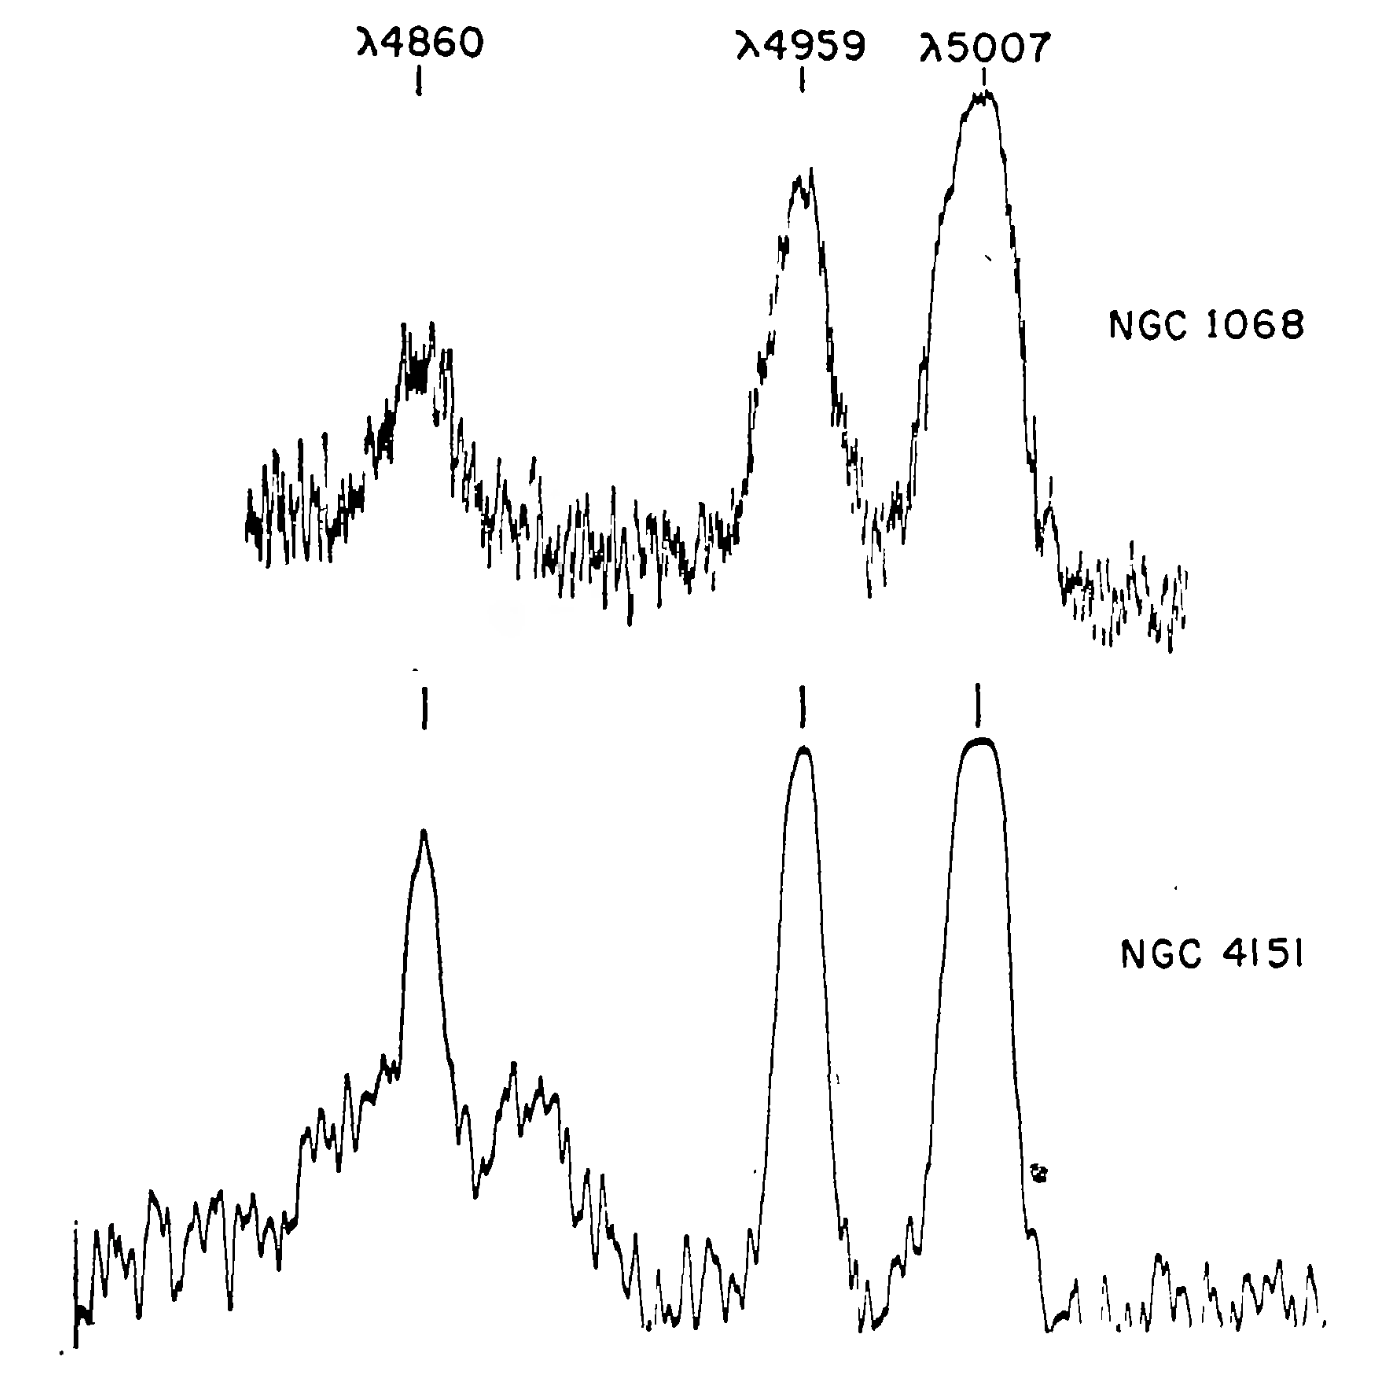
\includegraphics{figures/introduction/seyfert1943_spectra.png}
    \caption[Emission-line profiles for NGC\;1068 and NGC\;4151 as presented by \citet{Seyfert1943}.]{H$\beta$ and [OIII]$\lambda\lambda4959,5007$ emission line profiles for NGC\;1068 and NGC\;4151, as presented by \citet{Seyfert1943}. A prominent broad component can be seen only in H$\beta$ (a permitted line) in NGC\;4151. \textit{Image credit: Carl Seyfert (\citealt{Seyfert1943}; edited by the present author)}.}
    \label{fig: introduction: historical_context: seyfert1943_spectra}
\end{figure}

\newpage
\subsection{The advent of radio astronomy}
\label{section: introduction: historical_context: radio_astronomy}

While working as an engineer for Bell Telephone Laboratories in the early 1930s, Karl Jansky\footnote{A detailed account of Jansky's work and the history of radio astronomy, based on publications and private communications, is given by \citet{Kellerman2023}, from which relevant details are given in this section.} investigated sources of noise affecting shortwave ($\lambda$\;\textless\;100\;m; $\nu$\;\textgreater\;3\;MHz), long-distance telephone communications. Starting in 1930, Jansky used a directional antenna that could rotate fully in azimuth, allowing him to determine the directions of different sources of noise. Working at a wavelength of 14.5\;m (20.5\;MHz), he detected transmissions from stations in South America and England, in addition to noise generated by both distant and local thunderstorms. Although the noise from the storms was dominant, Jansky was also able to detect another source that did not correspond to known weather events. The apparent direction of the peak of this noise changed with the time of day and year, and its source was unclear until Jansky consulted his friend Melvin Skellet, a PhD student in astronomy, who recognised that its position corresponded to the Galactic plane of the Milky Way.

Although Jansky had --- for the first time in history --- observed the night sky at a different wavelength to the optical, his results attracted little attention. A later press release led to wider recognition, after which he published papers on his so-called `star noise' in \textit{the Proceedings of the IRE} \citep{Jansky1933b} and \textit{Nature} \citep{Jansky1933a}. However, his responsibilities at Bell Laboratories took precedence, and he was unable to comprehensively investigate cosmic radio emission further.

While the astronomical community took effectively no notice of Jansky's work, other radio engineers did. Perhaps most notable of these was Grote Reber, who built a steerable parabolic dish dedicated to studying cosmic radio emission and mapped the sky at various frequencies. Reber's radio maps showed not only diffuse emission along the Galactic plane, but also several maxima \citep{Reber1944}, including one in the constellation Cygnus (the maximum in which would later be labelled Cygnus\;A).

Radio astronomy flourished after the conclusion of the Second World War as a result of an abundance of experienced radar technicians, radio experts, and former military equipment. Of particular interest to the early radio astronomy community was Cygnus\;A, which was identified as a discrete source during the war \citep{Hey1946}. Subsequent sea-cliff interferometric observations by J.G. Bolton \& G.J. Stanley identified other discrete sources in addition to Cygnus\;A (see \citealt{Kellerman2023}, Chapter 3), and interest quickly grew in these `radio stars'. However, their natures were poorly understood, and the low astrometric precision of early radio observations made the identification of optical counterparts difficult.

Despite this, through the use of sea-cliff interferometry, \citet{Bolton1949} were able to achieve sufficiently precise radio-source positions to identify the optical counterparts of three of them: Taurus A was identified with the Crab Nebula (M1); Virgo A was identified with M87 (a large elliptical galaxy with an elongated structure\footnote{The narrow, elongated structure in M87 was first identified at optical wavelengths by \citet{Curtis1918}, who noted "a curious straight ray" associated with the object, which is now recognised as an AGN jet. For the definition of AGN jets used in this thesis, see the \hyperref[chapter: definitions]{Definitions} section.}), and Centaurus A was identified with the elliptical galaxy NGC\;5128. Further accurate radio-interferometric positions by \citet{Smith1951} allowed \citet{Baade1954} to identify the optical component of Cygnus\;A: a galaxy at a redshift of $z=0.056$ presenting forbidden lines (such as [OIII], [OII], [NeV]) and H$\alpha$ with relatively broad line widths ($\sim$400\;km\;s$^{-1}$), similar to Seyfert nuclei. It thus became clear that many discrete radio sources were extragalactic, and the correspondingly large distances implied unprecedented luminosities. By the end of the 1950s, it was appreciated that `radio galaxies' such as these should be detectable up to high redshifts --- this provoked great interest among astronomers, since source number counts at the corresponding distances could discriminate between competing cosmological models.

Also at this time, spectroscopic follow-up observations of the radio source 3C\;48 --- a stellar-like object with faint nebulosity --- revealed broad emission lines that did not correspond to any known atomic or ionic transition, and optical imaging showed excess ultraviolet (UV)-emission (see discussion in \citealt{Shields1999}). Similar broad lines and UV-excesses were later associated with other radio sources, which were labelled Quasi-Stellar Sources (QSS) or Quasi-Stellar Objects (QSO); eventually, this terminology was shortened to `quasars'\footnote{The term `quasar' was first used by \citet{Chiu1964}, however, it was first defined in scientific literature --- along with the terms `QSO' and `QSS` --- by \citet{Schmidt1970}, who defined them as being ``objects of starlike appearance ... that exhibit redshifts much larger than those of ordinary stars''. For the definition of the term `Quasar' used throughout this thesis, see the \hyperref[chapter: definitions]{Definitions} section.}. The true nature of these objects was discovered when Maarten Schmidt performed optical follow-up observations of the radio source 3C\;273, an accurate position and angular extent for which had been recently established by \citet{Hazard1963} during a lunar occultation. In optical imaging, 3C\;273 appeared as a 13th-magnitude star, while the spectra revealed that the `star' had broad lines at unfamiliar wavelengths, similar to those identified with 3C\;48 previously. Noting a series of four emission lines of decreasing flux, Schmidt realised that the lines could be explained as the Balmer recombination series of hydrogen if they were redshifted by $z=0.16$. This in turn allowed for the identification of the UV emission line Mg\;II\;$\lambda2798$ in both 3C\;273 and 3C\;48; the redshift of the latter was determined to be $z=0.37$. These results were published in adjacent papers in the journal \textit{Nature} \citep{Hazard1963, Schmidt1963, Oke1963, Greenstein1963}, and quasars were thus identified as active galaxies with spectra similar to those seen in Seyfert nuclei, albeit with higher luminosities.

However, it was not clear what the mechanism responsible for the extreme luminosities of quasars and Seyfert galaxies was, nor how it could be responsible for the observed spectra. An early attempt to understand this was made by \citet{Woltjer1959} who, based on the observed fraction of spiral galaxies that have Seyfert-like nuclei, the fact that the nuclei are spatially-unresolved in imaging, and a virial argument involving observed line widths, estimated that the high luminosities of observed Seyfert nuclei were generated by a 10$^{8-9}$\;M$_\odot$ object in a compact volume (\textless\;100\;pc$^{-3}$). Five years later, \citet{Salpeter1964} and \citet{Zeldovich1964} proposed that this could be understood as accretion onto supermassive black holes (SMBHs), as a non-rotating SMBH could release 0.057c$^2$ of energy per unit mass: sufficient to power the observed luminosities of quasars and Seyfert nuclei.

This argument was popularised by \citet{LyndenBell1969}, who postulated that `dead quasars' (i.e. quiescent SMBHs) should be common in the nuclei of all galaxies, given the energy output of quasars seen at higher redshifts (corresponding to earlier cosmological times). Moreover, \citet{LyndenBell1969} determined that the emission expected from accretion disks around active SMBHs could photoionise gas in galactic nuclei, leading to the spectra observed in quasars. Therefore, by the late 1960s, not only were the central AGN-engines of active galaxies (e.g. Seyferts and quasars) beginning to be understood, but it was appreciated that their unprecedented luminosities may impact their host galaxies, motivating studies in the following decades that sought to understand the nature of this impact.

\subsection{Narrow-line studies of active galaxies}
\label{section: introduction: historical_context: nlr_studies}

\subsubsection{The connection between ionised gas and radio structures}
\label{section: introduction: historical_context: nlr_studies: early_outflows}

An important characteristic of active galaxies, identified since the earliest spectroscopic observations (e.g. \citealt{Slipher1917, Campbell1918, Seyfert1943}; Figure \ref{fig: introduction: historical_context: seyfert1943_spectra}), is the presence of narrow (full width at half maximum (FWHM)\;\textless\;1000\;km\;s$^{-1}$) and broad (FWHM\;\textgreater\;1000\;km\;s$^{-1}$) emission-line profiles. Due to their associated velocities being a significant fraction of the speed of light, the broad lines received much attention in studies of active galaxies, while the narrow lines were of less interest (see discussion in \citealt{Krolik1984}). 

While \citet{Seyfert1943} recognised that narrow line broadening (100\;\textless\;FWHM\;\textless\;1000\newline km\;s$^{-1}$) was due to the Doppler shifting of lines within the objects, the physical implication of this was first considered by \citet{Burbidge1958}, who noted that the line widths corresponded to velocities that were much higher than the galactic escape velocities and therefore ``the interstellar gas in the nuclear regions must be constantly escaping from the galaxy as a whole". This was subsequently supported by a study of the inner regions ($r$\;\textless\;2\;kpc) of the archetypal Seyfert galaxy NGC\;1068, which showed that the observed line widths implied velocities that are more than three times that of the escape velocity on these scales \citep{Burbidge1959}. 

Higher-spatial-resolution optical spectroscopy at different spatial positions and position angles (PAs) allowed for the identification of discrete clouds responsible for the observed line broadening in active galaxies (particularly NGC\;1068 and NGC\;4151: e.g. \citealt{Merle1968, Anderson1970, Glaspey1976}). These clouds were found to have velocity shifts in the range 100\;\textless\;$v$\;\textless\;1000\;km\;s$^{-1}$: higher than the escape velocity at their radii ($r$\;\textless\;$500$\;pc). This supported the idea of an `expansion' of gas away from the nuclei, an interpretation that was refined by \citet{Heckman1981}, who argued that observed asymmetries in the narrow-line profiles in a sample of 36 active galaxies were due to AGN-driven radial outflows of gas (see also \citealt{Grandi1977} and \citealt{Heckman1983}).

Simultaneously, studies throughout the 1970s began to investigate the physical conditions (including temperatures, densities, reddenings, and compositions) of the narrow-line-emitting gas, with a particular focus on determining how it is ionised. The prevailing candidate ionisation mechanisms were photoionisation via radiation emitted by AGN accretion disks (e.g. \citealt{MacAlpine1972, Baldwin1975, Shields1975, OsterbrockKoski1976, Ferland1979}) and astrophysical shock-waves propagating through the interstellar mediums (ISMs) of the host galaxies (e.g. \citealt{Cox1972, Koski1976, Fosbury1978, Penston1978}). Combined with the presence of outflowing gas, this indicated that AGN were having a significant impact on the central regions of galaxies.

Also in this time period, new radio observatories (such as the Westerbork Synthesis Telescope, the National Radio Astronomy Observatory 300-foot radio telescope, and the Mullard Radio Astronomy Observatory) were used to perform both large surveys of the local AGN population and detailed studies of individual objects. The radio surveys performed with these facilities found that galaxies with Seyfert nuclei had radio luminosities that were higher than those of normal (quiescent) spiral galaxies, but less than those of the `radio galaxies' discovered in the decades prior \citep{vanderKruit1973, Sramek1975}. The advent of higher-spatial-resolution radio observations in the 1980s, permitted by new facilities such as the Very Large Array (VLA) and Multi-Element Radio Linked Interferometer Network (MERLIN), revealed that the radio morphologies of Seyfert galaxies often consisted of two or more components, connected by fainter emission on arcsecond (kiloparsec) scales (e.g. \citealt{Wilson1980, Wilson1982, Pedlar1983, Pedlar1984, Ulvestad1984}; Figure\;\ref{fig: introduction: historical_context: nlr_studies: wilson1982_ngc1068_15ghz}) --- similar to what had previously been identified on much larger scales in powerful radio galaxies such as Cygnus A \citep{Jennison1959}. These double and triple radio structures were interpreted as synchrotron emission produced by AGN jets \citep{Wilson1980}: fast (up to tenths of the speed of light), collimated streams of plasma that are launched from AGN accretion disks along the spin axis of the central SMBH (see \citealt{Rees1984} for a contemporary review). In this scenario for Seyfert galaxies, the radio emission observed at the position of the optical nucleus (the core) originates from the central AGN engine, while the extended radio component(s) (the lobes) represent the termination point of the jet and/or prominent interactions of the jet with the ISM of the host galaxy \citep{Wilson1980, Sanders1984}.

\begin{figure}[!t]
    \centering
    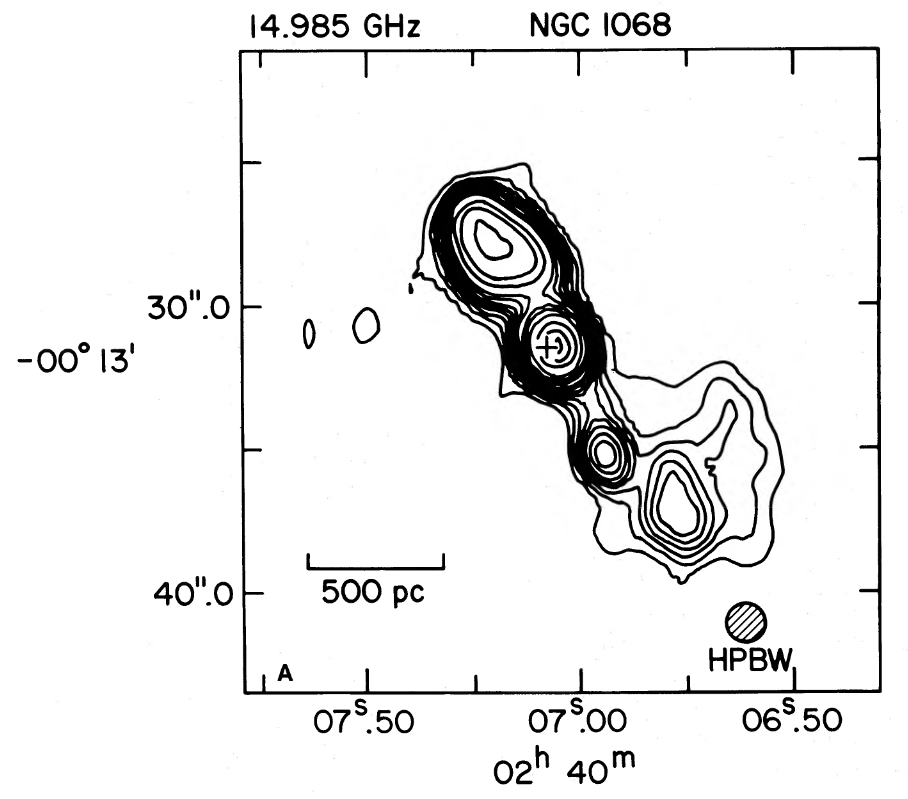
\includegraphics[width=0.8\linewidth, trim={0 0 -3cm 0}, clip]{figures/introduction/ulvestad1982_ngc1068_15ghz.png}
    \caption[14.985\;GHz radio map of the inner kiloparsecs of the Seyfert galaxy NGC\;1068 (as presented by \citealt{Wilson1982}), showing a linear radio structure.]{14.985\;GHz map of the inner kiloparsecs of the Seyfert galaxy NGC\;1068, showing a linear, triple radio structure consisting of a core (coincident with the optical nucleus, marked by the cross) and two radio lobes. The contours are 1, 2, 3, 4, 5, 6, 8, 10, 15, 20, 30, 50, 70 and 90\;per\;cent of 192.5\;mJy\;beam$^{-1}$. \textit{Image credit: \citet{Wilson1982}}.}
    \label{fig: introduction: historical_context: nlr_studies: wilson1982_ngc1068_15ghz}
\end{figure}

Concurrently, multi-wavelength studies utilising both optical and radio observations discovered empirical correlations between the radio and narrow-line properties of Seyfert galaxies, notably between 1.4\;GHz (21\;cm) and [OIII] luminosity \citep{deBruyn1978}, and 1.4\;GHz luminosity and [OIII] line width \citep{Wilson1980}. Furthermore, high-spatial-resolution observations revealed that in many cases, the major axes of linear radio structures and optical narrow-line emission were aligned (\citealt{Ulvestad1981}; see Table 2 in \citealt{Wilson1985}). This implied a physical relationship between the radio- and narrow-line-emitting material; although the nature of this connection was not clear, suggestions were made that plasma jets were interacting with the ISMs of host galaxies, ionising the gas and accelerating outflows (see Section 3 of \citealt{Wilson1985}).

The relationship between narrow-line-emitting gas and radio structures was first directly investigated by \citet{Whittle1988}, who used spatially-resolved spectroscopic observations of 10 Seyfert galaxies that presented double or triple linear radio structures. It was found that, not only was the [OIII] and H$\beta$ line emission strongly spatially associated with the radio structures, but their line profiles were particularly complex at the locations of bright radio emission. The derived narrow-line velocities were high (150\;\textless\;$v$\;\textless\;1000\;km\;s$^{-1}$), with the highest velocities found at the position of the enhanced radio emission. This indicated that the gas was more kinematically disturbed at these locations, and thus that prominent AGN-driven outflows are associated with radio structures on kiloparsec-scales.

\subsubsection{The unified scheme of AGN and ionisation cones}
\label{section: introduction: historical_context: nlr_studies: unified scheme}

As seen in the spectra presented by \citet{Seyfert1943} (Figure \ref{fig: introduction: historical_context: seyfert1943_spectra}), there exists a dichotomy in AGN regarding the widths of permitted and narrow lines. Some objects, termed Seyfert\;1s (Sey\;1, later generalised to Type 1 AGN) present narrow forbidden lines and broad permitted lines, while others (Seyfert 2, or Sey\;2; generalised to Type 2 AGN) show narrow forbidden and permitted lines (see \citealt{Khachikian1971}). The underlying mechanism responsible for this was confirmed by \citet{Antonucci1985}, who used spectropolarimetric measurements of the Sey\;2 galaxy NGC\;1068 to demonstrate the presence of polarised broad permitted lines. This indicated that the source of the broad permitted lines --- known as the broad line region (BLR) --- also existed in Type 2 AGN, but was obscured by a torus-like structure (which may be clumpy: \citealt{Nenkova2002, Nenkova2008}; see Section\;2.3 of \citealt{Netzer2015}), and confirmed that Type 1 and Type 2 AGN were intrinsically the same phenomenon, only viewed at different angles with respect to the observer (Figure\;\ref{fig: introduction: historical_context: nlr_studies: unified_scheme}).

\begin{figure}[!ht]
    \centering
    \includegraphics[width=\linewidth]{figures/introduction/unified_scheme.png}
    \caption[Schematic of the unified scheme of AGN.]{Schematic of the unified scheme of AGN. The central supermassive black hole (SMBH; $r\sim10$--100\;AU), accretion disk ($r\sim1000$--10,000\;AU), jet, and obscuring torus ($r\sim0.1$--10\;pc) are labelled with solid black arrows; the locations of the broad line region (BLR; $r\sim100$--1000\;AU) and narrow line region (NLR; $r\sim0.1$--10\;kpc) are also labelled. The dashed arrows show the lines of sight that result in an AGN being observed as Type\:1 or Type\:2. Not to scale.}
    \label{fig: introduction: historical_context: nlr_studies: unified_scheme}
\end{figure}

Optical observations of the narrow line regions (NLRs; kiloparsec-scale regions of narrow-line emission) of Seyfert galaxies in the late 1980s and early 1990s revealed interesting morphologies: the narrow-line-emitting gas appeared to be distributed in conical shapes, the apexes of which corresponded to the position of active nuclei (\citealt{Pogge1988, Pogge1989, Pogge1990, Tadhunter1989, Cecil1990, Miller1990, Evans1991}). In many cases, there was evidence of two cones lying in opposite directions along the same axis --- known as a bicone --- and in almost all cases the (bi)cones were aligned with the radio axes of the objects.

The launch of the Hubble Space Telescope (HST) in 1990\footnote{A grounding error in the HST's primary mirror produced significant spherical aberration in observations until it was fixed during a service mission in 1993. Despite this, the telescope was still scientifically useful for studies of nearby AGN during this period.} allowed optical studies of unprecedented spatial resolution, which showed that the NLR quiescent and outflowing gas structures were much more complex than indicated by earlier observations. While many authors argued, based on spatially-resolved gas kinematics and conditions, that outflows in Seyfert galaxies are driven via shocks induced in the ISM by radio jets (e.g. \citealt{Taylor1992, Bower1995, Capetti1995a, Capetti1995b, Axon1998}), others argued that radiation pressure from accretion disks also contributed to outflow acceleration (and is perhaps the dominant driving mechanism). In the latter scenario, this driving is done either by fast ($\sim$0.1\;$c$) winds launched close to the nucleus (called nuclear winds) that shock the cold ISM on larger scales and accelerate outflows (e.g. \citealt{Cecil1990}), or by direct radiation pressure acting on the NLR gas (e.g. \citealt{Crenshaw2000_N1068, Crenshaw2000_N4151, Kaiser2000}).

\subsection{AGN-driven outflows and galaxy evolution}
\label{section: introduction: historical_context: galaxy evolution}

Early studies which interpreted complex narrow-line profiles in Seyfert galaxies as being due to `expansion' (e.g. \citealt{Walker1968, Anderson1970, Glaspey1976}), and later outflows of gas (e.g. \citealt{Grandi1977, Heckman1981}), indicated that AGN were having an impact on the central kiloparsecs of galaxies. However, the first recognition that AGN-driven outflows may play an important role in how galaxies evolve was by \citet{Sanders1988}. Noting that ultra luminous infrared galaxies (ULIRGs; $L_\mathrm{IR}$\;\textgreater\;$10^{12}$\;L$_\mathrm{\odot}$: \citealt{Sanders1988, Sanders1996}) present merger-like morphologies and host bright nuclei, \citet{Sanders1988} proposed that these objects contained obscured quasar-like nuclei which drive high-mass gas outflows that remove or destroy the obscuring dust. In this scenario, ULIRGs transition into quasars, forming an evolutionary sequence.

However, the main impetus for studying AGN-driven outflows came in the mid-1990s, when empirical scaling relations between SMBH masses and host-galaxy bulge properties (luminosity, velocity dispersion, and stellar mass; Figure\;\ref{fig: introduction: historical_context: galaxy_evolution: ferrarese2000_mbh_vdisp}) were discovered \citep{Kormendy1995, Magorrian1998, Gebhardt2000, Ferrarese2000}. The form of these correlations could be readily explained by SMBHs and galactic bulges accreting the same material (i.e. gas inflows to the centres of galaxies), however, this could not explain their tightness --- an additional mechanism was thought to be required. Outflows driven by AGN were first invoked to be this additional mechanism by \citet{Silk1998}, who created an analytic model that required a small fraction of AGN luminosity to couple to the ISMs of host galaxies, driving galaxy-wide outflows which set the tightness of the observed scaling relations. AGN-driven outflows subsequently became the basis of further analytic models that could explain the empirical SMBH-bulge scaling relations (e.g. \citealt{Fabian1999, King2003}).

\begin{figure}
    \centering
    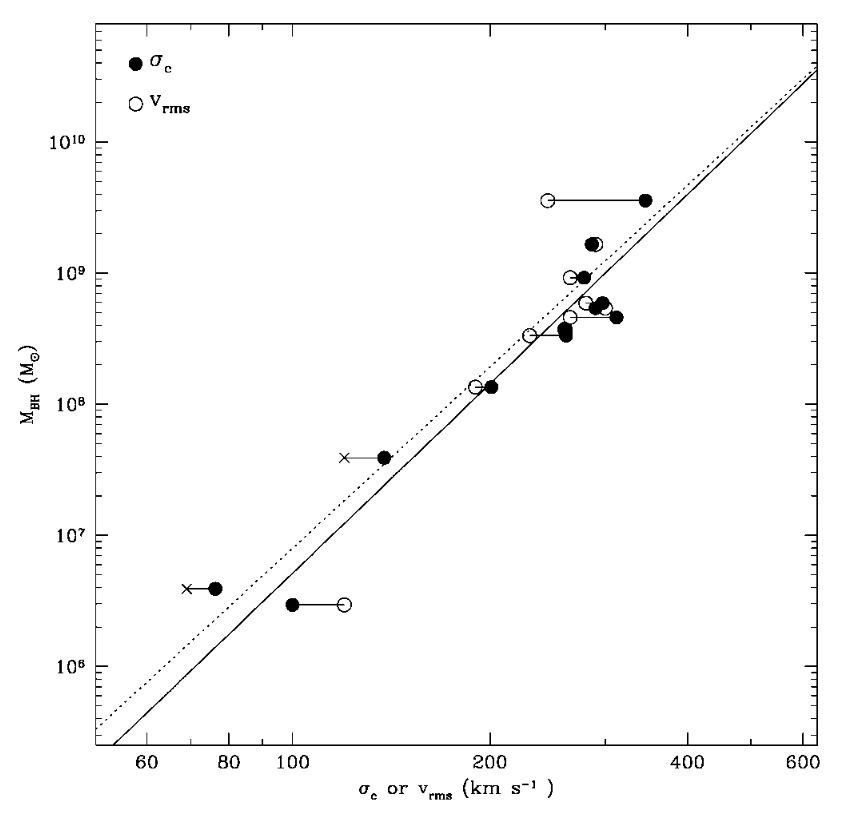
\includegraphics[width=0.9\linewidth]{figures/introduction/ferrarese2000_mbh_vdisp.png}
    \caption[Empirical scaling relation between supermassive black hole mass and galactic bulge stellar velocity dispersion, presented by \citet{Ferrarese2000}.]{Empirical scaling relation between supermassive black hole mass and stellar velocity dispersion ($\sigma_c$: filled circles) or root-mean-square (rms) velocity ($v_{rms}$: hollow circles; crosses represent lower limits) as presented by \citet{Ferrarese2000}. The dashed and solid lines represent the best linear fits. \textit{Image credit: \citet{Ferrarese2000}}.}
    \label{fig: introduction: historical_context: galaxy_evolution: ferrarese2000_mbh_vdisp}
\end{figure}

In addition, AGN also began to be invoked to explain several other observed features of galaxies and their environments (see \citealt{Cattaneo2009} for a contemporary review), such as AGN jets heating and preventing the cooling of highly-ionised, hot X-ray-emitting gas that is observed in and around galaxy clusters \citep{McNamara2007, Gaspari2013} and the luminosity function of the local galaxy population \citep{Benson2003}. The collective impact that AGN are thought to have on their host galaxies is referred to as AGN feedback, which is now a crucial component of models of galaxy evolution (including detailed hydrodynamical simulations: e.g. \citealt{DiMatteo2005, Springel2005, Hopkins2010}; and cosmological simulations: e.g. \citealt{Schaye2015, Dave2019, Zinger2020}). While AGN-driven outflows are thought to be required to explain SMBH-bulge scaling relations, they are also now commonly considered to be an important aspect of AGN feedback in general, and therefore have become the focus of an increasing number of studies over the past thirty years (Figure\;\ref{fig: introduction: historical_context: galaxy_evolution: harrison2018_abstracts}).

\begin{figure}
    \centering
    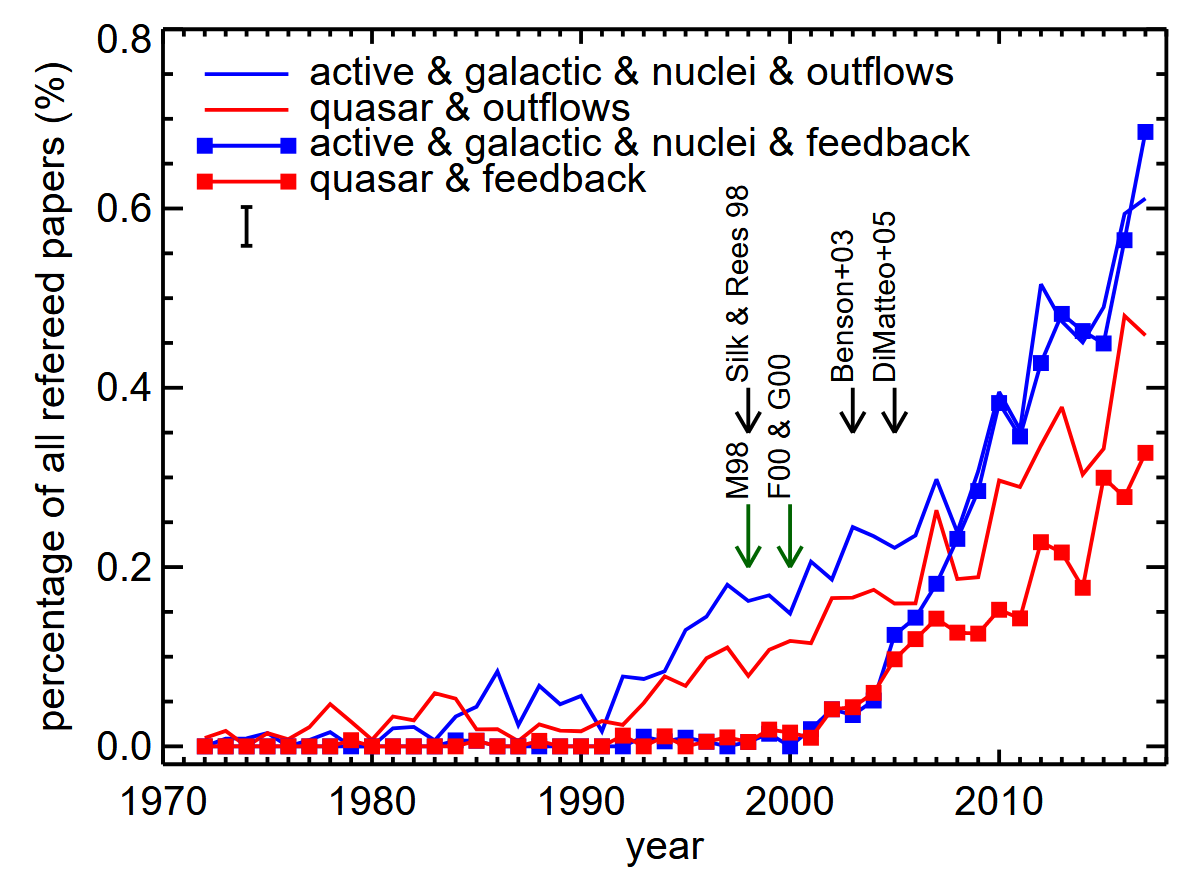
\includegraphics[width=0.85\linewidth]{figures/introduction/harrison2018_abstracts.png}
    \caption[Cumulative number of published AGN-driven outflow studies since the early 1970s, taken from \citet{Harrison2018}.]{Percentage of peer-reviewed publications from 1970 to 2018 that contain the keywords given in the legend (top left) in their abstracts. The publication dates of key studies (M98: \citealt{Magorrian1998}; F00: \citealt{Ferrarese2000}; G00: \citealt{Gebhardt2000}; \citealt{Benson2003, DiMatteo2005}) which produced a significant increase in interest of AGN-driven outflows are marked with vertical arrows. \textit{Image credit: \citealt{Harrison2018}.}}
    \label{fig: introduction: historical_context: galaxy_evolution: harrison2018_abstracts}
\end{figure}

\newpage
\section{AGN-driven outflows}
\label{section: introduction: outflows: introduction}

The first hydrodynamical simulation of the impact of AGN-driven outflows on galaxy evolution was performed by \citet{DiMatteo2005}, who modelled a major galaxy merger with SMBHs as sink particles. These SMBHs injected thermal energy ($E_\mathrm{feed}$) into the ISM of the merger as
\begin{equation}
    E_\mathrm{feed}=\epsilon_\mathrm{f}\eta_\mathrm{r}\dot{M}_\mathrm{BH}c^2
    \label{eq: introduction: outflows: introduction: dimatteo2005_efeed}
\end{equation}
where $\eta_\mathrm{r}$ is the radiative efficiency of the SMBH accretion disk, $\dot{M}_\mathrm{BH}$ is the accretion rate onto the SMBH, and $c$ is the speed of light. Here, $\epsilon_\mathrm{f}$ is a free parameter known as the coupling efficiency (or coupling factor): the fraction of radiation coupled to the ISM of the host galaxy. In this model, the coupling of radiation to the ISM launches galaxy-wide ($r$\;\textgreater\;5\;kpc) outflows, heating and expelling gas needed to form stars, hence suppressing star formation. 

The coupling efficiency in the \citet{DiMatteo2005} simulation was set to the value required ($\epsilon_\mathrm{f}=0.05=5$\;per\;cent) to reproduce the normalisation of the observed relation between SMBH mass and bulge stellar velocity dispersion (known as the $M$-$\sigma$ relation; Figure\;\ref{fig: introduction: historical_context: galaxy_evolution: ferrarese2000_mbh_vdisp}). Subsequent theoretical work also invoked galaxy-wide, AGN-driven outflows, with each setting a different value of this free parameter to reproduce the normalisation of empirical relations (typically 0.5\;\textless\;$\epsilon_\mathrm{f}$\;\textless\;10\;per\;cent: \citealt{Springel2005,Hopkins2010}). In the 2010s, large-scale cosmological simulations incorporated a similar approach to their AGN-feedback prescriptions, requiring a fraction of energy produced by accreting SMBHs in galactic centres to be coupled to host galaxies (e.g. $\epsilon_\mathrm{f}=0.15=15$\;per\;cent for EAGLE and Horizon-AGN: \citealt{Schaye2015, Dubois2016}), restricting star formation and therefore reproducing the observed properties of the local galaxy population. 

Motivated by these theoretical models, observational studies of AGN-driven outflows often interpret the coupling efficiency as being the ratio between outflow kinetic power ($\dot{E}_\mathrm{kin}$: kinetic energy per unit time) and AGN bolometric luminosity ($L_\mathrm{bol}$):

\begin{equation}
    \epsilon_\mathrm{f}=\frac{\dot{E}_\mathrm{kin}}{L_\mathrm{bol}}.
    \label{eq: introduction: outflows: introduction: e_f}
\end{equation}

Therefore, in attempts to verify the models --- and hence the role of AGN-driven outflows in galaxy evolution --- a large number of studies in the past twenty-five years have focused on measuring coupling efficiencies in this way and comparing them to the free parameter set by models. Many observational studies have derived coupling efficiencies that fall in the range required by theoretical work (0.5\;\textless\;$\epsilon_\mathrm{f}$\;\textless\;10\;per\;cent: e.g. \citealt{Liu2013, Harrison2014, Cicone2014, Fiore2017}), however, there are several major sources of uncertainty associated with this approach which render its validity unclear.

Principally, observationally-derived outflow kinetic powers are not well constrained: due to many factors, commonly-determined values may be incorrect by several orders of magnitude. Furthermore, the validity of direct comparisons to theoretical models using coupling efficiencies is unclear, as is the robustness of interpretations that are made from such comparisons regarding the impacts of AGN-driven outflows on host galaxies (see discussion in \citealt{Harrison2018}); largely, this is because it is unclear exactly \textit{how} AGN accelerate outflows. In the following sections, I review and explain these uncertainties.

\subsection{Uncertainties regarding outflow energetics}
\label{section: introduction: outflows: energetics}

\subsubsection{The multi-phase nature of outflows}
\label{section: introduction: outflows: energetics: multi-phase}

The ISM is observed in a range of gas phases: regimes of different temperatures and conditions, ranging from hot and highly-ionised to cold and molecular. Similarly, AGN-driven outflows have been observed in multiple phases, corresponding to distinct temperatures and compositions of the emitting gas (see \citealt{Cicone2018} for a review). Different phases are observed with tracers at different wavelengths --- Table\;\ref{tab: introduction: outflows: energetics: multi-phase: outflow_phases} presents the phases considered in this thesis, and examples of their observational tracers.

\begin{table}[!t]
    \vspace*{-1cm}
    \centering
    \centerline{
    {\renewcommand{\arraystretch}{4}
    \begin{tabular}{ccc}
        Phase & Temperature range & Observational tracers \\
        \hline
        \parbox{4cm}{\hspace*{\fill} Highly ionised \hspace*{\fill}} & \textgreater\;$10^6$\;K & \parbox{8cm}{Hard X-ray ($E_\gamma$\;\textgreater\;6\;keV) absorption lines \\ \hspace*{\fill} (e.g. Fe\;XXV, Fe\;XXVI); \hspace*{\fill} \\ \hspace*{\fill} X-ray continuum \hspace*{\fill}} \\
        Warm ionised & 10,000--30,000\;K & \parbox{8cm}{\hspace*{\fill} UV, optical, near-infrared, and \hspace*{\fill} \\ \hspace*{\fill} mid-infrared emission lines \hspace*{\fill} \\ \hspace*{\fill} (e.g. [OIII]$\lambda\lambda4959,5007$, H$\beta$, Pa$\beta$, \hspace*{\fill} \\ \hspace*{\fill} [SII]$\lambda\lambda6717,6731$, HeI, [O IV]\;25.9\;$\mu$m) \hspace*{\fill}} \\
        Warm molecular & $\sim2000$\;K & \parbox{8cm}{\hspace*{\fill} Near-infrared roto-vibrational \hspace*{\fill} \\ \hspace*{\fill} emission lines of H$_2$ \hspace*{\fill} \\ \hspace*{\fill} (e.g. H$_2$(1--0)S(1)\;2.212\;$\mu$m, \hspace*{\fill} \newline \hspace*{\fill} H$_2$(2--1)S(1)\;2.247\;$\mu$m) \hspace*{\fill}} \\
        Neutral atomic & 100--2000\;K & \parbox{8cm}{\hspace*{\fill} Radio emission lines  (e.g. HI\;21\;cm line), \hspace*{\fill} \\ \hspace*{\fill} optical NaID absorption lines \hspace*{\fill} \\ \hspace*{\fill} (NaID$\lambda\lambda$5890,5896) \hspace*{\fill}} \\
        Cold molecular & 10--300\;K & \parbox{8cm}{\hspace*{\fill} Radio/sub-mm emission \& absorption lines \hspace*{\fill} \\ \hspace*{\fill} (e.g. CO(1--0), CO(2--1), HCN, OH) \hspace*{\fill}} \\
    \end{tabular}
    }
    }
    \caption[The gas phases of AGN-driven outflows that are considered in this thesis.]{The gas phases of AGN-driven outflows that are considered in this thesis, their approximate temperatures, and examples of their observational tracers (wavelength regime and example spectral features).}
    \label{tab: introduction: outflows: energetics: multi-phase: outflow_phases}
\end{table}

Since the majority of studies use observations of only one phase (commonly the warm-ionised gas, due to it producing prominent optical emission lines), it is not clear which outflow phase is dominant in terms of mass and kinetic power. In a relatively small number of active galaxies, the properties of outflows in multiple phases have been quantified (e.g. \citealt{Morganti2005, Holt2011, Tadhunter2014, Riffel2015, Feruglio2015, Morganti2016, Finlez2018, Fluetsch2019}); in some objects, these phases have been seen to be co-spatial and co-kinematic, indicating that they form part of the same outflow (Figure\;\ref{fig: introduction: outflows: energetics: multi-phase: morganti2015_ic5063_multiphase}: \citealt{Tadhunter2014, Morganti2015}).

\begin{figure}[!t]
    \centering
    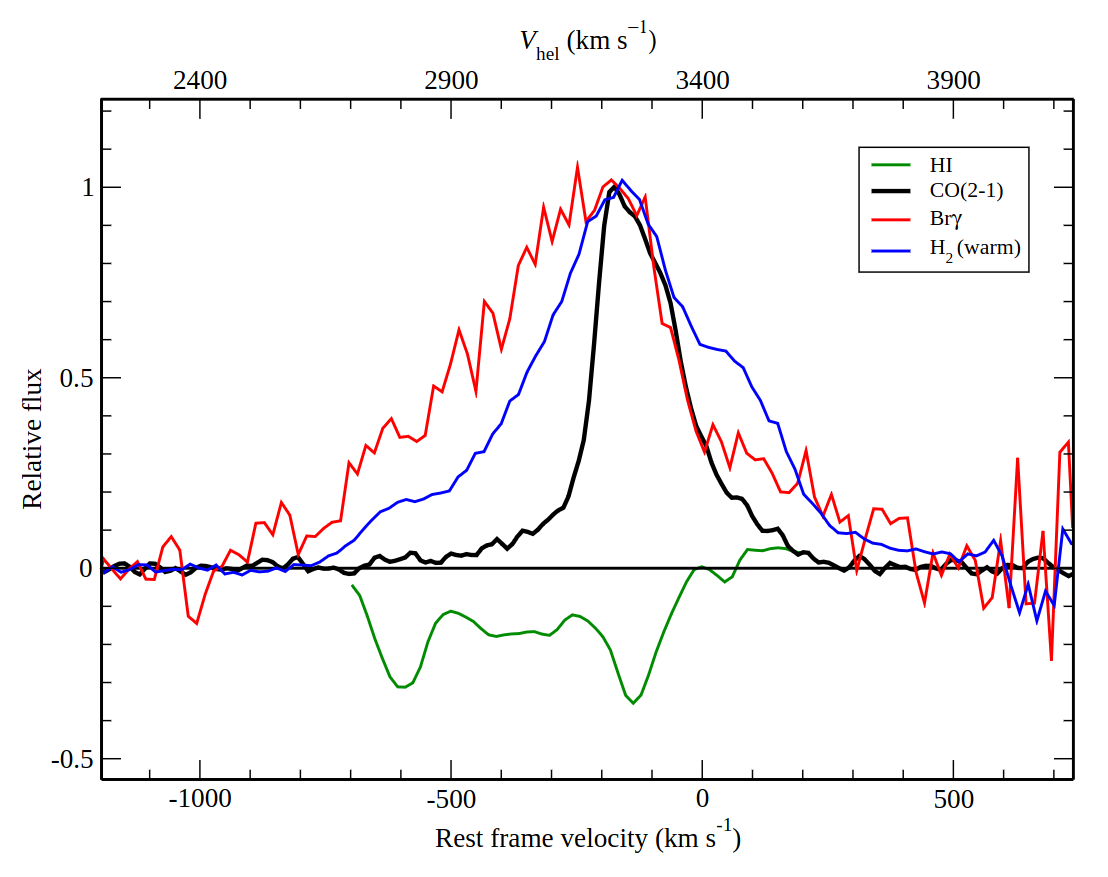
\includegraphics[width=\linewidth]{figures/introduction/morganti2015_ic5063_multiphase.png}
    \caption[Lines arising from different outflow phases in IC\;5063 \citep{Morganti2015}, indicating a co-spatial, co-kinematic multi-phase outflow.]{Line velocity profiles tracing different phases of outflowing gas at the same location in the active galaxy IC\;5063. The red line shows the Br$\gamma$ emission-line profile (warm ionised; \citealt{Tadhunter2014}), the blue line shows the H$_2$(1--0)S(1)\;2.212\;$\mu$m emission-line profile (warm molecular; \citealt{Tadhunter2014}), the green line shows the HI 21\;cm absorption-line profile (neutral atomic; \citealt{Morganti1998}), and the black line shows the CO(2-1) emission-line profile (cold molecular; \citealt{Morganti2015}). Each phase presents outflowing (yet distinct) kinematics, potentially indicating that they are part of the same outflow. \textit{Image credit: \citealt{Morganti2015}}.}
    \label{fig: introduction: outflows: energetics: multi-phase: morganti2015_ic5063_multiphase}
\end{figure}

While some studies present evidence that the cold molecular phase is dominant in terms of mass and kinetic power (i.e. \citealt{Morganti2005, Cicone2014, GarciaBurillo2014}), this has only been determined for a small number of galaxies. Therefore, since the majority of studies only focus on a single phase, it is imperative that the relative masses and powers of multiple phases are comprehensively determined to ensure that \textit{total} outflow kinetic powers are not significantly underestimated.

Moreover, the physical relation between different outflow phases is not understood, nor is it clear how molecular gas can be accelerated to observed outflow velocities ($v$\;\textgreater\;500\;km\;s$^{-1}$) without being dissociated. Understanding this is crucial, as it is required to make quantitative predictions regarding multi-phase outflows. One suggestion is that the various phases in a given gas cloud are accelerated together directly by radiation pressure or cosmic rays \citep{Booth2013, Costa2018, Hopkins2020}, however, in this scenario, it is not clear why the molecules are not photo-disassociated. Other studies propose a solution to this by arguing that the colder, molecular phases are entrained in warmer gas, preventing molecule dissociation \citep{Scannapieco2015, Gaspari2017, Gronke2020}. 

An alternative is that the outflow acceleration mechanism heats the gas to the hot ionised phase ($T$\;\textgreater\;$10^6$\;K), destroying the molecules in the process; as the gas cools post-acceleration, it forms the cooler phases \textit{in-situ}, including the formation of molecules \citep{Wang1995, Silich2003, Tadhunter2014, Zubovas2014, Costa2015, Thompson2016, Richings2021}. A major problem with understanding this scenario is the complexity (and associated difficulty) of modelling molecule formation in the ISM: it is not clear if molecules can form in outflowing-gas conditions on the (highly uncertain) timescales required. In this context, it is interesting to note that recent modelling supports molecule formation and cooling being a sufficiently fast process in outflowing gas \citep{Richings2021}.

Overall, the mass and energy contributions of (and the physical relation between) different outflow phases are not clear --- in order to elucidate this situation, detailed, multi-wavelength observations of multi-phase outflows and their acceleration mechanisms are required.

\subsubsection{Electron densities of warm-ionised outflows}
\label{section: introduction: outflows: energetics: electron_densities}

The most commonly observed outflow phase is warm ionised gas, as many emission lines arising from this phase are present in optical spectra of AGN (Table\;\ref{tab: introduction: outflows: energetics: multi-phase: outflow_phases}). Therefore, many studies that compare outflow kinetic powers to those required by models of galaxy evolution only consider warm-ionised outflow energetics (masses, mass outflow rates, kinetic powers, and coupling efficiencies: e.g. \citealt{Liu2013, Rose2018, Tadhunter2019}). Typically, this is done by first calculating the warm-ionised outflow mass using the measured luminosity of a recombination line of hydrogen ($L(H)$) with
\begin{equation}
    M_\mathrm{out, ion} = \frac{L(H)m_\mathrm{p}}{\alpha^\mathrm{eff}_\mathrm{H}hv_\mathrm{H}n_e},
    \label{eq: introduction: outflows: energetics: mout}
\end{equation}
where $M_\mathrm{out, ion}$ is the mass of the outflowing warm-ionised gas, $m_\mathrm{p}$ is the proton mass, $\alpha^{eff}_{H}$ is the Case B recombination coefficient for the chosen recombination line of hydrogen, $v_\mathrm{H}$ is the frequency of the recombination line, and $n_e$ is the electron density of the emitting gas. This is then used to calculate the mass passing through a given surface area per unit time, known as the mass outflow rate:
\begin{equation}
    \dot{M}_\mathrm{out, ion} = A\cdot\frac{M_\mathrm{out, ion}\;v_\mathrm{out}}{R},
    \label{eq: introduction: outflows: energetics: mout_rate}
\end{equation}
where $v_\mathrm{out}$ is the outflow velocity, $R$ is the outflow radius, and $A$ is a constant that accounts for assumptions regarding outflow geometry and radial density profiles (see Section 2 of \citealt{Veilleux2020}). Finally, the outflow kinetic power is calculated using
\begin{equation}
    \dot{E}_\mathrm{kin, ion} = \frac{1}{2}{\dot{M}_\mathrm{out, ion}(v^2_\mathrm{out} + 3\sigma^2)},
    \label{eq: introduction: outflows: energetics: ekin}
\end{equation}
where $\sigma$ is the velocity dispersion ($\sigma\sim\mathrm{FWHM}$/2.355), which may be interpreted as the range of velocities present \textit{within} a spatially-unresolved region of outflowing gas; a multiplicative factor of three is commonly used with this term to account for the velocity dispersion in three dimensions (see \citealt{Rupke2005b}). Typically, the coupling efficiency (taken to be the ratio of outflow kinetic power to the host AGN bolometric luminosity: Equation\;\ref{eq: introduction: outflows: introduction: e_f}) is then determined and compared to the requirements of theoretical models --- if the observed value is consistent with (or above) these requirements, then the interpretation is often that the outflows have a significant impact on the evolution of the host galaxy.

The largest source of uncertainty when calculating outflow energetics in this way is the electron density of the outflowing gas. Traditionally, the flux ratio of emission lines in a doublet arising from either the SII or OII ion is used (namely [SII](6717/6731) and [OII](3726/3729)): the lines involved in these ratios have similar (but different) critical densities\footnote{The critical density of a transition is defined as the density at which the rate of collisional de-excitation from the upper energy level becomes approximately equal to the collisional excitation rate of electrons to the upper energy level (see Chapter\;5 of \citealt{Osterbrock2006}).}, and so the ratios have a strong dependence on electron density (Figure\;\ref{fig: introduction: outflows: energetics: warm_ionised: sii_ratio})\footnote{The [SII](6717/6731) and [OII](3726/3729) flux ratios also have a dependence on electron temperature. Therefore, when calculating electron densities with these ratios, electron temperatures are either measured using other line ratios (e.g. [OIII](5007+4959)/4363) or assumed to be those typical of the warm ionised phase ($\sim$10,000\;K); see Chapter\;5 of \citet{Osterbrock2006}.}.

\begin{figure}[!ht]
    \centering
    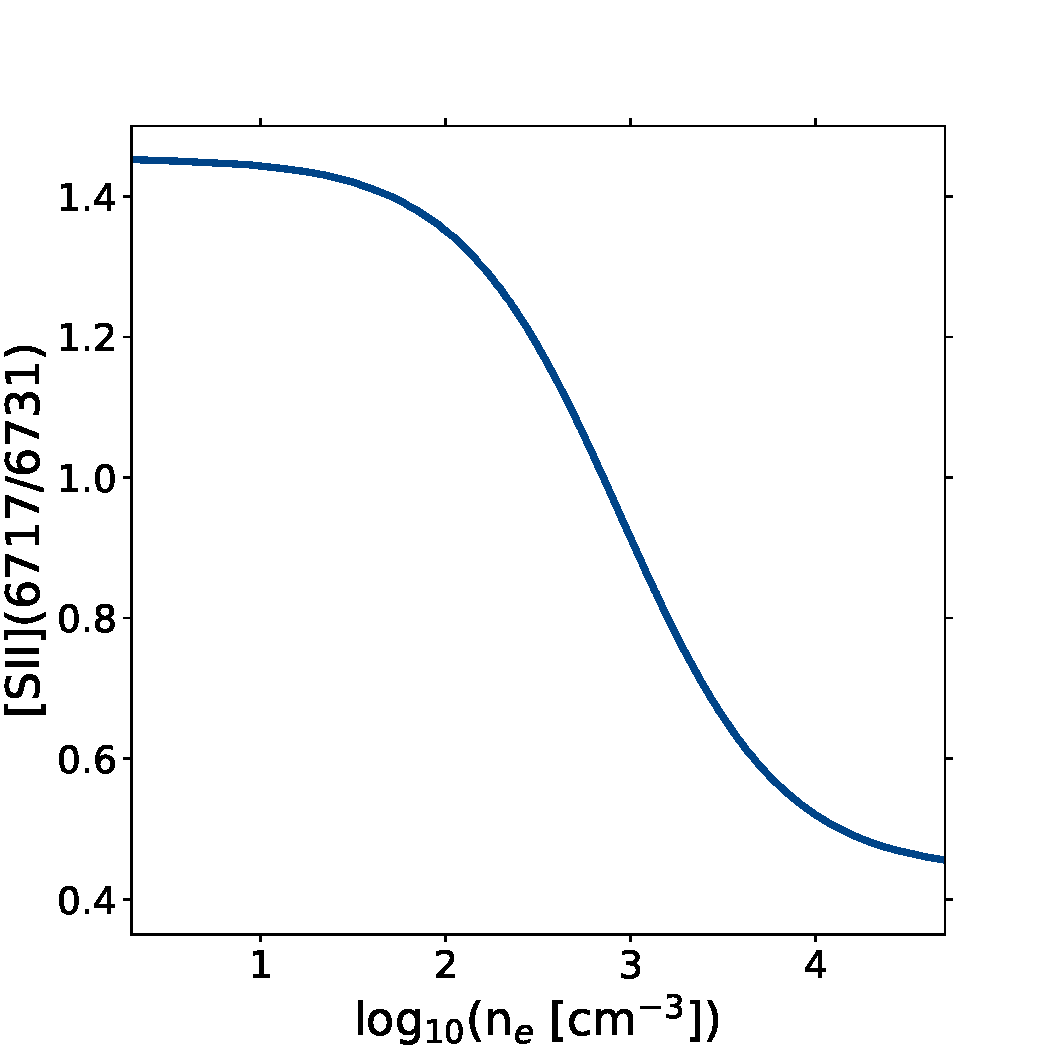
\includegraphics[width=0.7\linewidth]{figures/introduction/sii_ratio.pdf}
    \caption[{Variation of the [SII](6717/6731) emission-line flux ratio with electron density.}]{Variation of the traditional [SII](6717/6731) emission-line flux ratio with electron density, modelled with the \textsc{PyNeb} \textsc{Python} module \citep{Luridiana2015} for an ionised gas of temperature $T_e=10,000$\;K. This commonly-used density diagnostic is only sensitive to densities in the range 2.0\;\textless\;log$_{10}$($n_e$[cm$^{-3}$])\;\textless\;3.5: above and below these limits, the curve becomes increasingly asymptotic, and the values derived from this technique saturate.}
    \label{fig: introduction: outflows: energetics: warm_ionised: sii_ratio}
\end{figure}

However, these traditional, commonly-used ratios are only sensitive up to electron densities of $n_e\sim10^{3.5}$\;cm$^{-3}$ --- above this limit, both of the lines involved are collisionally suppressed, and the values of the ratios saturate. If, in reality, outflow densities are greater than $n_e\sim10^{3.5}$\;cm$^{-3}$, then this technique will underestimate true values. Crucially, since outflow masses (Equation\;\ref{eq: introduction: outflows: energetics: mout}), mass outflow rates (Equation\;\ref{eq: introduction: outflows: energetics: mout_rate}), kinetic powers (Equation\;\ref{eq: introduction: outflows: energetics: ekin}), and coupling efficiencies (Equation\;\ref{eq: introduction: outflows: introduction: e_f}) depend inversely on the electron density, this means that these derived properties would be overestimated. Therefore, it is notable that many studies which determine high outflow kinetic powers (i.e. $\epsilon_\mathrm{f}$\;\textgreater\;0.5\;per\;cent) also estimate or assume low electron densities ($n_e$\;\textless\;10$^{3.5}$\;cm$^{-3}$: e.g. \citealt{Kraemer2000II, Nesvadba2006, Harrison2014, Fiore2017}). Furthermore, the separation between the lines in the [SII] and [OII] doublets is small, and in the case of outflow kinematics --- in which line widths are typically intermediate-to-high (FWHM\;\textgreater\;500\;km\;s$^{-1}$) --- the lines are often blended. This introduces significant degeneracy in measuring the flux ratios, therefore preventing precise electron density determinations.

In the past decade, novel techniques of electron-density estimation have been developed which are sensitive to a wider range of values than the traditional [SII] and [OII] ratios. For example, \citet{Baron2019b} present a technique which uses the dimensionless ionisation parameter

\begin{equation}
    U=\frac{Q}{4{\pi}r^2cn_e},
    \label{eq: introduction: outflows: energetics: u}
\end{equation}

\noindent
where $Q$ is the number of ionising photons emitted by the AGN per second, and $r$ is the radial distance of the gas outflow from the AGN. In this method, the ionisation parameter is determined using emission-line ratios, $Q$ is derived from the bolometric luminosity of the AGN, and the outflow radial distance is determined from modelling the mid-infrared (MIR) spectral energy distribution (SED) of the AGN (see \citealt{Baron2019a}). Therefore, Equation\;\ref{eq: introduction: outflows: energetics: u} can be used to estimate the electron density, which \citet{Baron2019b} find to be in the range 3.0\;\textless\;log$_{10}$($n_e$\;[cm$^{-3}$])\;\textless\;6.2 for a sample of 234 Type\;2 AGN --- several orders of magnitude above the upper density limit of the traditional [SII] and [OII] ratios. Similarly, complex, multi-ionisation-component (i.e. multiple values of $U$) photoionisation modelling that utilises the measured fluxes of many emission lines has produced a wide range of electron densities when applied to outflows in nearby active galaxies (2.0\;\textless\;log$_{10}$($n_e$\;[cm$^{-3}$])\;\textless\;7.0: \citealt{Collins2009, Crenshaw2015, Revalski2021}; see also \citealt{Revalski2022}). 

Of particular note is a technique pioneered by \citet{Holt2011} using the [SII](4068 + 4076)/(6717 + 6731) and [OII](3726 + 3729)/(7319 + 7331) ratios, which involve the \textit{total} fluxes of the traditional [SII]$\lambda\lambda$6717,6731 and [OII]$\lambda\lambda$3726,3729 doublets in addition to the higher-critical-density transauroral \citep{Boyce1933} [SII]$\lambda\lambda$4068,4076 and [OII]$\lambda\lambda$7319,7331 doublets. By comparing the measured values of these ratios to predictions of photoionisation modelling, electron densities and reddenings can be derived simultaneously. Importantly, this technique is sensitive to a wider range of electron densities (2.0\;\textless\;log$_{10}$($n_e$\;[cm$^{-3}$])\;\textless\;5.5) than the traditional [SII](6717/6731) and [OII](3726/3729) ratios, but requires less-detailed observations (and is less computationally expensive) than the ionisation-parameter-based method presented by \citet{Baron2019b} and complex photoionisation modelling \citep{Collins2009, Crenshaw2015, Revalski2021}. Moreover, unlike the traditional [SII] and [OII] ratios, the transauroral-line method uses the \textit{total} fluxes of emission-line doublets instead of the fluxes of individual lines \textit{within} the doublets, obviating issues arising from degeneracy due to broad line widths.

In the past 13 years, the transauroral ratios have been used to measure gas densities in the range 3.0\;\textless\;log$_{10}$($n_e$\;[cm$^{-3}$])\;\textless\;5.5 in active galaxies of different types \citep{Holt2011, Rose2018, Santoro2018, Spence2018, RamosAlmeida2019, Santoro2020, Davies2020, Speranza2022}. These densities are up to two orders of magnitude higher than could be measured with the traditional ratios, and, correspondingly, modest outflow kinetic powers and coupling efficiencies have been derived ($\epsilon_\mathrm{f}$\;\textless\;0.5\;per\;cent). However, these studies have used spatially-unresolved observations, often with a single aperture covering the outflow region. Consequently, it has been argued that the transauroral lines are emitted by different clouds than those that emit other key diagnostic lines such as [OIII]$\lambda\lambda$4959,5007 and H$\beta$, and therefore that the derived densities are not representative of the outflowing gas (\citealt{Sun2017}; but see discussions in \citealt{Rose2018} and \citealt{Spence2018}). Since the outflow masses and kinetic powers resulting from transauroral-line-derived densities are much below those typically found for the warm ionised phase (and are potentially far below the values required by models of galaxy evolution), this situation needs to be investigated in detail to conclusively determine if the transauroral lines are valid tracers of outflowing gas.

\subsubsection{A low-surface-brightness, high-mass, warm ionised outflow component}

The techniques and studies described above for the warm ionised phase trace relatively dense ($n_e$\;\textgreater\;3.0\;cm$^{-3}$) gas in the central regions ($r$\;\textless\;2\;kpc) of active galaxies. While these studies find modest outflow masses and kinetic powers, it is possible that there also exists a tenuous ($n_e$\;\textless\;3.0\;cm$^{-3}$), low-surface-brightness, spatially-extended ($r$\;\textgreater\;5\;kpc) warm-ionised outflow component that the observations were not sensitive to. \citet{Spence2018} estimate that such a component could be ten times more massive than dense outflows in the centres of galaxies, despite only contributing 10\;per\;cent to the luminosities of key emission lines; this may form the powerful, galaxy-wide component of the outflows invoked by models of AGN in galaxy evolution \citep{DiMatteo2005,Springel2005,Schaye2015}. Therefore, deep, spatially-resolved, galaxy-scale studies of active galaxies with known small-scale ($r$\;\textless\;2\;kpc) outflows need to be performed in order to identify any potential spatially-extended, low-surface brightness counterparts.

\subsection{Outflow kinematics and geometry}
\label{section: introduction: outflows: kinematics_and_geometry}

\subsubsection{Outflow kinematics}
\label{section: introduction: outflows: kinematics_and_geometry: kinematics}

Determining accurate outflow kinematics is crucial, as the derived mass outflow rates (Equation\;\ref{eq: introduction: outflows: energetics: mout_rate}) and kinetic powers (Equation\;\ref{eq: introduction: outflows: energetics: ekin}) have square and cubic dependencies on velocity shifts (and dispersions), respectively. Kinematics are often derived in spectroscopic studies of AGN-driven outflows: as noted by \citet{Seyfert1943}, the line widths seen in the NLRs of nearby active galaxies are readily explainable by clouds of different velocities causing the Doppler-shifting of emission lines. In modern observational studies, prominent emission lines are used to determine kinematics --- perhaps the most commonly used is the [OIII]$\lambda\lambda$4959,5007 doublet, which is bright in typical AGN spectra, does not present broad wings from the BLR (Section\;\ref{section: introduction: historical_context: nlr_studies: unified scheme}) and, with the exception of extreme cases, is not blended with other emission lines. 

For a static cloud in a narrow line region, the dominant line-broadening effect would be Doppler motions of gas moving with a Maxwellian distribution of velocities, which is described by a Gaussian profile. Therefore, it is generally assumed that individual velocity components of a given emission-line profile follow a Gaussian distribution of wavelengths (or velocities). Consequently, many studies fit one or more Gaussian profiles (accounting for different velocity components) to outflow emission-line profiles to model the kinematics of the gas (e.g. \citealt{VillarMartin1999, Crenshaw2000_N1068, Das2005, Holt2011, Mullaney2013, Rose2018, Tadhunter2019}) --- often, the wavelength difference between the mean of a Gaussian component and the rest wavelength of the line is used to calculate velocity shift ($v$), and the width of the Gaussian component (either $\sigma$ or FWHM) is taken as a measure of the distribution of velocities within the cloud.

However, there are challenges to robustly interpreting outflow line profiles in terms of kinematics, mainly regarding projection effects: broad, complex line profiles may be produced by an ensemble of clouds with a large internal velocity dispersion, or by a system of clouds that is unresolved to the observer and has a small local velocity dispersion, and for which the clouds are flowing with a wide range of angles relative to the observer's line of sight (LOS). In terms of kinematics, complex line profiles therefore present a degeneracy: both of the described cases could give rise to an identical line profile, but the derived outflow velocities will change significantly depending on the assumed scenario. In an attempt to break this degeneracy, some studies use non-parametric approaches to de-project outflow kinematics. An example of this is percentile velocities, which involve measuring the velocity that contains a certain percentage of the total line flux under the assumption that the outflow velocity is the same in all directions (and that the local velocity dispersion is small), and therefore the far wings of line profiles (the maximum projected velocities) represent clouds moving along the line of sight (e.g. \citealt{CanoDiaz2012, Harrison2014, Rose2018}). In this approach, a velocity that contains 90\;per\;cent of the line flux would be represented by $v_{90}$. Similarly, some studies define non-parametric line widths based on the difference between two percentile velocities, for example $W_{80}=v_{90}-v_{10}$ (e.g. \citealt{Harrison2014, Venturi2021}). An example of these non-parametric approaches to measuring outflow kinematics is shown for a mock emission-line profile in Figure\;\ref{fig: introduction: outflows: kinematics: hbeta_v05_v95_w90}.

\begin{figure}[!t]
    \centering
    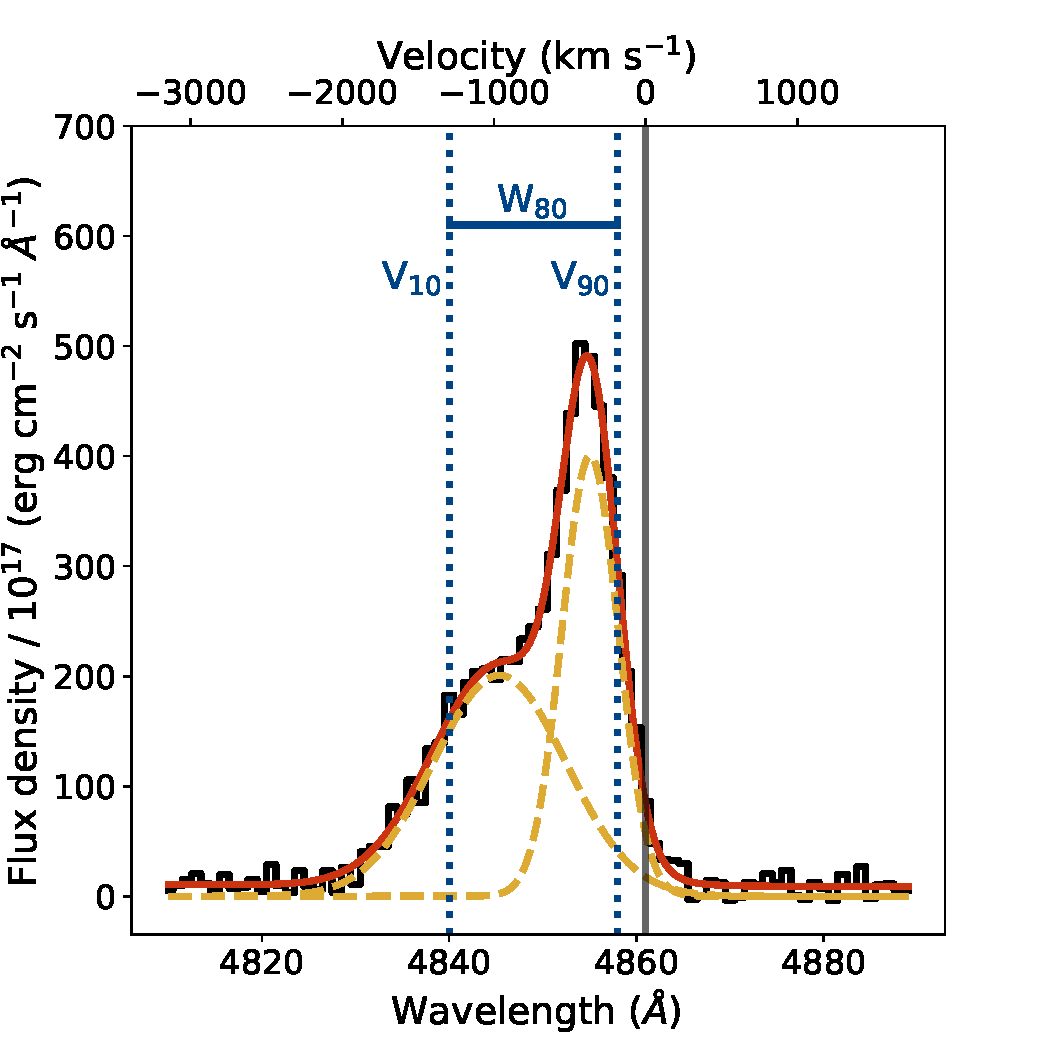
\includegraphics[width=0.7\linewidth]{figures/introduction/hbeta_v10_v90_w80.pdf}
    \caption[Examples of non-parametric percentile velocity shifts and widths for a simulated H$\beta$ line.]{Examples of non-parametric percentile velocity shifts ($v_\mathrm{10}$, $v_\mathrm{90}$: vertical dotted blue lines) and width ($W_\mathrm{80}$) for a simulated H$\beta$ line profile. The black line shows the simulated H$\beta$ emission, the solid red line shows the total fit, the dashed orange lines show the two individual Gaussian components required to fit the line profile, and the vertical solid grey line shows the rest wavelength of H$\beta$.}
    \label{fig: introduction: outflows: kinematics: hbeta_v05_v95_w90}
\end{figure}

The ideal approach to account for projection effects (and therefore determining robust kinematics) would be detailed modelling of NLR kinematics. For several nearby Seyfert galaxies, this has been done by fitting biconical, radial outflow models to kinematics derived from high-spatial-resolution HST spectra \citep{Crenshaw2000_N1068, Crenshaw2000_N4151, Das2005, Das2006, Das2007, Revalski2021}. However, such an approach requires detailed, spatially-resolved observations (and so is restricted to bright, nearby galaxies), is time-expensive, and relies on assumptions regarding outflow acceleration mechanisms, which themselves are not clear. Therefore, care must be taken when deciding how to measure outflow kinematics, and the method used should be considered when making physical interpretations based on derived outflow kinematics and energetics.

\subsubsection{Outflow spatial extents}
\label{section: introduction: outflows: kinematics_and_geometry: spatial_extents}

Models of galaxy evolution predict outflows that extend to galaxy-wide scales ($r$\;\textgreater\;5\;kpc: e.g. \citealt{Silk1998, DiMatteo2005, King2010, Curtis2016, Costa2018}). In contradiction to this, studies of nearby active galaxies that use long-slit spectroscopic observations with a technique called spectroastrometry --- which involves measuring the spatial centroid position of an emission line as a function of velocity along the slit \citep{Bailey1998} --- have found that warm-ionised outflows extend up to a few kiloparsecs (at maximum) from the central AGN \citep{Carniani2015, Spence2016, VillarMartin2016, Santoro2018, Santoro2020}, in agreement with the results of direct HST imaging \citep{Fischer2018, Tadhunter2018} and spectroscopy \citep{Das2005, Das2006, Das2007, Tadhunter2019}. In contrast, some optical integral field unit (IFU) studies have found outflows to be galaxy-wide \citep{Fu2009, Westmoquette2012, Liu2013, Harrison2014, Wylezalek2017}; since the observations used in these studies are ground-based, it has been suggested that the beam-smearing effects of atmospheric seeing artificially spread compact outflow emission from the central regions across the IFU field of view. This may have contributed to --- or been entirely responsible for --- the observed galaxy-wide outflow extents. Furthermore, \citet{Husemann2016} demonstrated that failure to account for beam smearing can result in overestimation of outflow kinetic powers by up to two orders of magnitude. Clearly, this situation needs to be investigated in detail, principally to determine the potential impact that atmospheric seeing can have on determinations of outflow spatial extents.

\subsection{Comparisons to models of galaxy evolution}
\label{section: introduction: outflows: comparisons_to_models}

In addition to the described uncertainties involved in calculating observationally-derived outflow kinetic powers, it is not clear if direct comparisons to the requirements of theoretical models of galaxy evolution are valid, or if interpretations drawn from such comparisons are robust. In this context, I highlight that, despite many observational studies attempting to verify models by comparing measured coupling efficiencies to those used in models, this parameter is not a \textit{predicted} quantity in such models: it is a free parameter that is set to reproduce the normalisation of the empirical SMBH-bulge scaling relations and properties of the local galaxy population.

Moreover, the AGN-feedback models used in cosmological simulations are not spatially resolved. One problem this can produce is numerical overcooling, which may be compensated for by increasing the required fraction of SMBH accretion power that is coupled to the ISM, potentially by orders of magnitude \citep{Weinberger2017} --- models that attempt to overcome this problem require a wide range of coupling efficiencies (0.04--30\;per\;cent: \citealt{Booth2009, Choi2012}). In addition, outflows may radiate a significant fraction of their energy post-acceleration, or decelerate under gravity, meaning that observationally-derived coupling efficiencies may be significantly lower than would be measured immediately after the outflow was launched. Furthermore, given that typical outflow dynamical timescales ($\sim$1--10\;Myr) may be similar to those of AGN cycles ($\sim$10--100\;Myr, although possibly much shorter in some cases: see \citealt{Morganti2017} for a review), it is unclear whether or not a given observed outflow was launched during the current epoch of AGN activity (the bolometric luminosity of which is used in coupling efficiency calculations). As argued by \citet{Harrison2018}, based on these arguments, it is not necessarily expected that coupling efficiency values required by models correspond to the measured ratio of outflow kinetic power to AGN bolometric luminosity, as is often assumed in observational outflow studies.

Therefore, direct comparisons of specific coupling efficiency values should be done with caution. Alternatively, \textit{qualitatively} comparing outflow properties derived from detailed observations to those predicted by tailored simulations of outflows in different object types may be an insightful (and perhaps complementary) approach. Detailed observational studies can also be used to inform the physics of the tailored models and the feedback prescriptions of cosmological simulations.


\subsection{Outflow acceleration mechanisms}
\label{section: introduction: outflows: acceleration_mechanisms}

A major barrier to robust comparisons of observations to theoretical models is that it is not clear how outflows are accelerated. AGN can launch outflows in two general ways: via radiation pressure from accretion disks, or via shocks induced in the ISM by jets. However, in many cases, both of these mechanisms can explain observed properties of the NLRs of local active galaxies, such as kinematics, spatial alignments between ionised gas and radio structures, and gas conditions \citep{Ulvestad1981, Wilson1985, Whittle1988, Cecil1990, Capetti1995a, Capetti1995b, Axon1998, Crenshaw2000_N1068, Crenshaw2000_N4151, Das2005, Das2006, Mukherjee2016, Mukherjee2018, Meena2021}. Furthermore, it is feasible that \textit{both} mechanisms could be present in a given galaxy, with their relative contributions to outflow acceleration and NLR ionisation/excitation being unclear.

\subsubsection{Radiatively-driven outflows}
\label{section: introduction: outflows: accleration_mechanisms: radiation}

The high luminosities produced by AGN accretion disks may impart significant radiation pressure on surrounding gas \citep{Castor1975, Abbott1982}, accelerating it via line-driving (bound-bound), continuum-opacity-driving (bound-free), and Thompson scattering (free-free) \citep{Arav1994, Murray1995, Proga1998, Proga2000}. In addition, dust may increase the effectiveness of radiation pressure driving on NLR gas at larger radii (i.e. where it is not vapourised by radiation: \citealt{Dopita2002, Fabian2006}). It has been proposed that these mechanisms can accelerate gas clouds in active galaxies to observed outflow velocities (up to several thousand kilometres per second; \citealt{Crenshaw2000_N1068, Crenshaw2000_N4151, King2003, Das2005, Das2006, Hopkins2010, King2010, MullerSanchez2011, Meena2021}). 

Two main variations of radiative driving are often invoked to explain observed NLR kinematics: radiation-driven winds launched close to the accretion disk that shock and accelerate the ISM on larger scales (e.g. \citealt{Elvis2000, Proga2000, King2003}), and radiation pressure directly accelerating colder NLR gas on kiloparsec-scales \textit{in situ} (e.g. \citealt{Das2007, Fischer2017, Revalski2018, Meena2021, Meena2023}). In an example of the former mechanism, \citet{Hopkins2010} propose that hot (4\;\textless\;log$_{10}(T [K])$\;\textless\;6), low-density ($n=1$--100\;cm$^{-3}$) gas close to the accretion disk ($r$\;\textless\;100\;pc) is radiatively accelerated to very high velocities ($v$\;\textgreater\;$10^4$\;km\;s\;$^{-1}$). As this high-velocity outflow impacts the colder, larger-scale ($r$\;\textgreater\;100\;pc) ISM, a series of shocks and dynamical instabilities cause it to mix with the colder gas, which produces an expansion in the direction perpendicular to the incident AGN radiation. The increased cross-section of the mixed cloud then leads to efficient, direct radiative driving. Very high-velocity nuclear winds such as those invoked in this model have been observed in the highly ionised phase (Table\;\ref{tab: introduction: outflows: energetics: multi-phase: outflow_phases}) with X-ray absorption lines \citep{Pounds2004, Lobban2011, Pounds2011, Tombesi2011}, and other studies making use of multi-wavelength observations have argued direct support for the importance of highly-ionised winds in driving larger-scale outflows \citep{Pounds2013, Feruglio2015}.

Tailored dynamical modelling that considers the balance of acceleration by radiation pressure and gravitational deceleration can reproduce the spatially-resolved outflow kinematics that are observed in the NLRs of some nearby active galaxies, lending support to radiation pressure being an important driving mechanism in these objects (\citealt{Crenshaw2000_N1068, Crenshaw2000_N4151, Das2005, Fischer2017, Revalski2018, Meena2021}). However, this requires high spatial- and spectral-resolution observations, and hence is limited to bright, nearby objects. Also, while this formalism can broadly explain the observed kinematics, in some cases, acceleration via shocks produced by jet-ISM interactions may be required \citep{Das2006, Das2007, Meena2023}. Furthermore, for several of the objects modelled in this way (e.g. NGC\;1068 and NGC\;4151), jet-ISM interactions alone may be able to explain observed spatial coincidence between radio structures and extreme NLR kinematics \citep{Capetti1995a, Capetti1995b, Axon1998, Das2006, May2017, May2020}, leaving the dominant acceleration mechanism unclear.

\begin{figure}[!t]
    \centering
    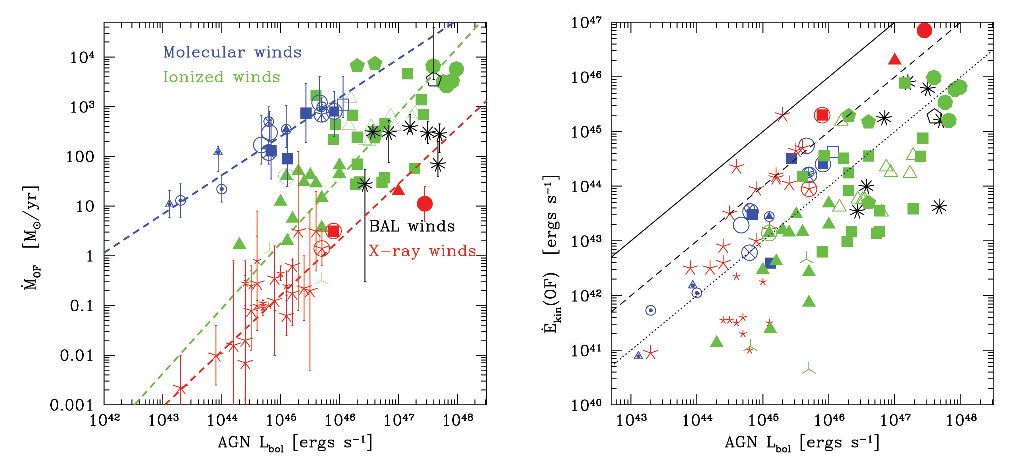
\includegraphics[width=\linewidth]{figures/introduction/fiore2017_mout_ekin_lbol.pdf}
    \caption[Observed multi-phase outflow scaling relations between outflow energetics and host AGN bolometric luminosity, as presented by \citet{Fiore2017}.]{Scaling relations between observed multi-phase outflow energetics (mass outflow rate: left; kinetic power: right) and AGN bolometric luminosity, produced by \citet{Fiore2017}. The red and black markers represent the energetics of highly-ionised X-ray and BAL (Broad Absorption Line; see review in \citealt{Gibson2009}) winds, green markers show energetics for warm-ionised outflows, and blue markers show the energetics of cold-molecular outflows. \textit{Image credit: \citet{Fiore2017}}.}
    \label{fig: introduction: outflows: acceleration_mechanisms: fiore2017_mout_ekin_lbol}
\end{figure}

Additional support for radiatively-driven outflows being common in active galaxies may be provided by statistical studies of a large number of objects. In particular, \citet{Fiore2017} collated observationally-derived mass outflow rates and kinetic powers for outflows and winds in the highly ionised, warm ionised, and cold molecular phases, and found scaling relations between these properties and AGN bolometric luminosity (Figure\;\ref{fig: introduction: outflows: acceleration_mechanisms: fiore2017_mout_ekin_lbol}). These relations may indicate that outflows in active galaxies are predominantly radiatively driven. However, it is unclear how observed mass outflow rates and kinetic powers of outflows driven by shocks from jet-ISM interactions would be expected to scale with bolometric luminosity. Furthermore, the uncertainties involved in deriving outflow energetics (Section\;\ref{section: introduction: outflows: energetics}) were not fully accounted for in producing these relations.

\subsubsection{Jet-driven outflows}
\label{section: introduction: outflows: accleration_mechanisms: jet_driven_outflows}

Feedback from AGN jets is commonly thought of in the context of powerful jets that extend far beyond the extents of host galaxies, such as those seen in Cygnus\;A \citep{Blandford1974, Carilli1991} and M87 \citep{Junor1999, Keiichi2012}. These jets reach the intergalactic or intracluster medium (IGM; ICM) and maintain the high temperatures and highly ionised states of halo gas, thus preventing catastrophic cooling and accretion to galaxy centres \citep{Binney1995, Soker2001, Best2006, McNamara2007, Gaspari2013}. On galaxy scales, these high-power jets are thought to pierce through the ISM without having a major impact or driving significant outflows (\citealt{Mukherjee2016}; see also \citealt{Scheuer1982, Hardee1990}). However, in the past two decades, theoretical work has demonstrated that lower-power jets ($P_\mathrm{jet}$\;\textless\;$10^{45}$\;erg\;s$^{-1}$) may instead provide an important source of feedback on galactic scales, as they are confined to the host galaxy medium for a longer time and hence affect a larger volume of the ISM (Figure\;\ref{fig: introduction: outflows: acceleration_mechanisms: mukherjee2016_high_low_power_jets}: \citealt{Mukherjee2016}; see also \citealt{Sutherland2007, Gaibler2011, Wagner2011, Mukherjee2016, Mukherjee2018}). In this scenario, the jets drive significant shocks into the ISM, heating and accelerating the gas and dissociating molecules. Modelling of jet-ISM interactions that includes both shock-ionisation induced by jets and photoionisation produced by AGN accretion disks predicts that the modelled ISM is predominantly shock-ionised \citep{Meenakshi2022a}, however, this has not been directly observationally verified.


\begin{figure}
    \centering
    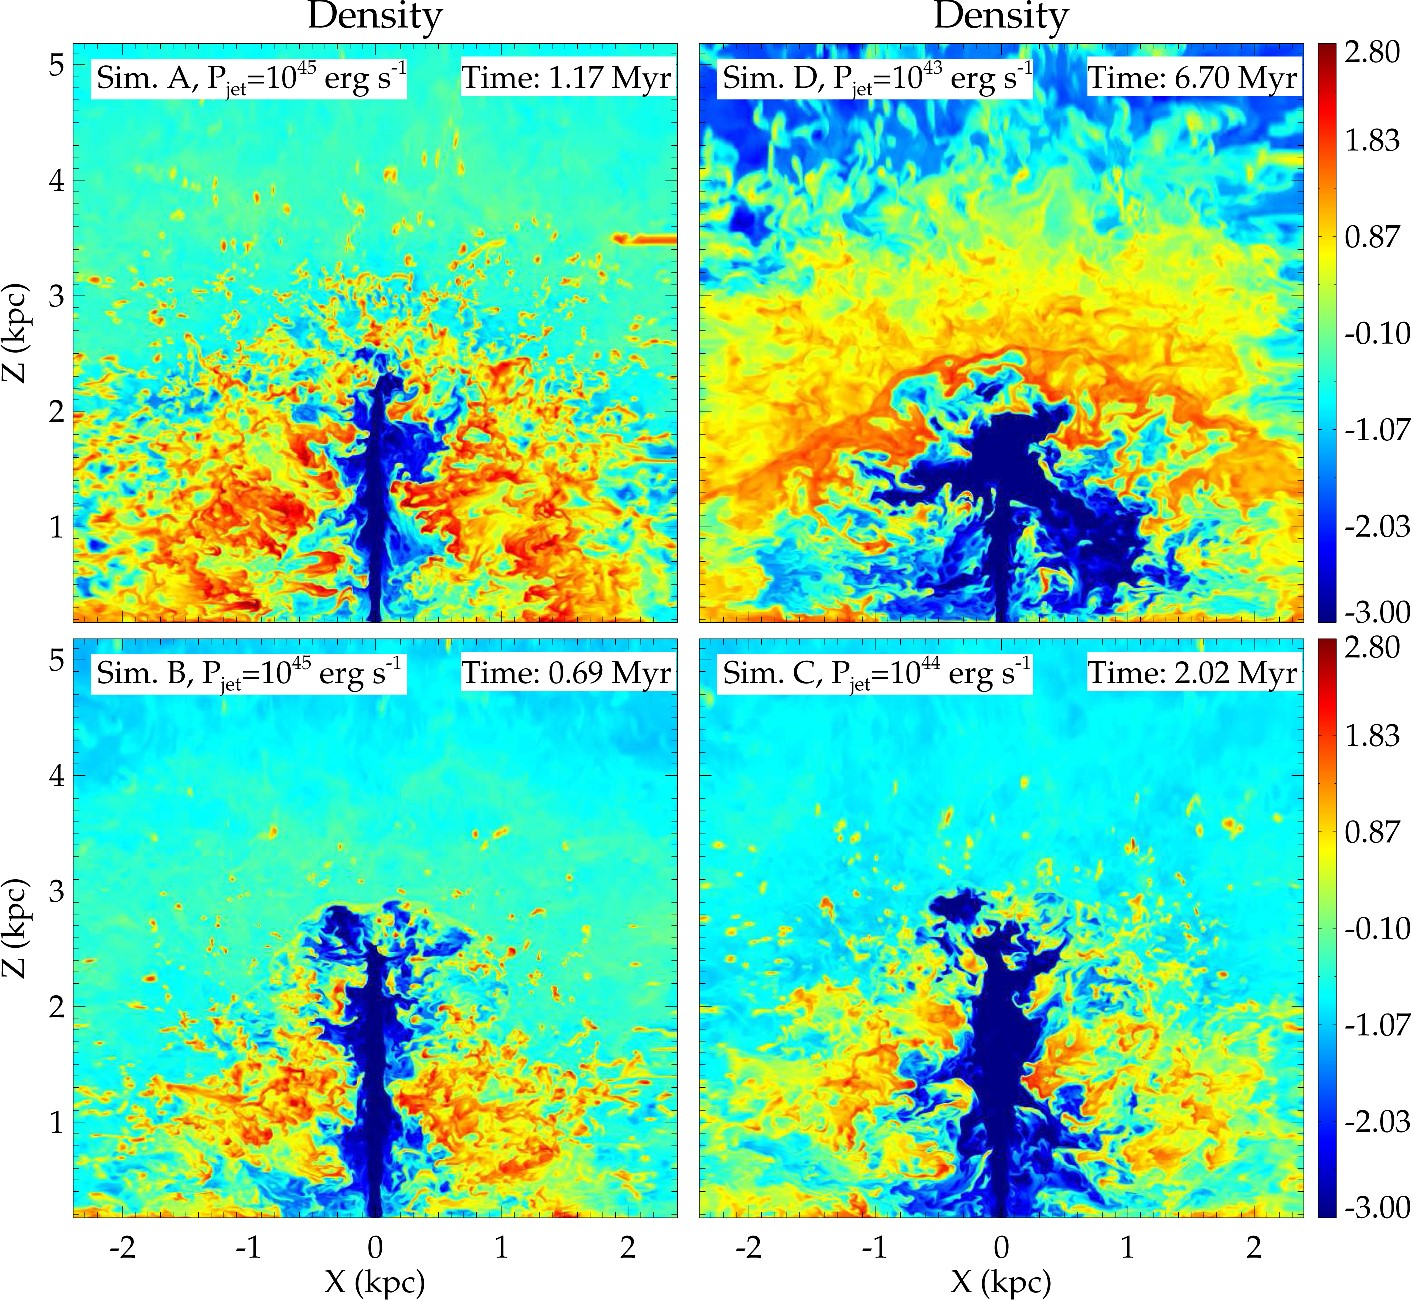
\includegraphics[width=\linewidth]{figures/introduction/mukherjee2016_high_low_power_jets.jpeg}
    \caption[Snapshots of hydrodynamic simulations by \citet{Mukherjee2016} of a higher- and lower-power jet propagating through an ISM.]{Gas density [cm$^{-3}$] in a two-dimensional plane for hydrodynamic simulations of jets of different powers ($P_\mathrm{jet}=10^{45}$\;erg\;s$^{-1}$: left panels; $P_\mathrm{jet}=10^{44}$\;erg\;s$^{-1}$: bottom-right panel; $P_\mathrm{jet}=10^{43}$\;erg\;s$^{-1}$: top-right panel) propagating through the ISM at different times. For the highest-power-jet case, the simulation in the top-left panel (`Sim. A') considers an ISM that is twice as dense as the ISM considered in `Sim. B' (bottom-left panel). In these models, the higher-power jets pierce through the ISM and escape confinement quickly, launching modest-mass outflows, while the lower-power jets remain confined for a longer time, cause more disturbance, and launch higher-mass outflows. \textit{Image credit: \citet{Mukherjee2016}}.}
    \label{fig: introduction: outflows: acceleration_mechanisms: mukherjee2016_high_low_power_jets}
\end{figure}

In addition to early outflow studies that found relations between disturbed NLR kinematics and radio structures (e.g. \citealt{Wilson1985, Whittle1988}), detailed observational studies have provided further evidence that jets drive outflows on galactic scales (e.g. \citealt{Morganti1998, Morganti2007, Nesvadba2008, Rosario2010a, Rosario2010b, Rosario2010c, Morganti2013_4c1250, Tadhunter2014, Mahony2016, May2017, Audibert2019, May2020, Venturi2021}). Of particular note are hydrodynamical simulations of AGN with low-power jets that can reproduce outflow properties derived from observational studies \citep{Morganti2015, Mukherjee2018, Audibert2023}.

In this context, it is interesting that a statistical study of a large sample of local ($z$\;\textless\;0.4), optically-selected AGN by \citet{Mullaney2013} found the broadest [OIII] emission-line profiles (indicative of more-prominent outflows) in objects of intermediate radio luminosity (23\;\textless\;log$_{10}$($L_\mathrm{1.4\;GHz}$[W\;Hz$^{-1}$])\;\textless\;25). Combined with the correlation between 1.4\;GHz luminosity and [OIII] line width previously found for Seyfert galaxies by \citet{Whittle1992c}, and the increased [OIII] line widths seen at the locations of prominent radio knots in the NLRs of Seyfert galaxies \citep{Whittle1988}, there is now considerable evidence that jets are an important outflow acceleration mechanism.

\subsubsection{Ionisation and excitation mechanisms as probes of acceleration}
\label{section: introduction: outflows: accleration_mechanisms: ionisation_and_excitation_mechanisms}

It is commonly assumed that different outflow acceleration mechanisms correspond to distinct gas ionisation or excitation mechanisms. For example, gas that has been directly radiatively-accelerated \textit{in situ} will have been subject to a significant flux of photo-radiation, therefore it is perhaps likely that at least the face of the cloud will be photoionised by the AGN. Conversely, material passing through a shock (driven into the ISM either by a fast nuclear wind or a jet) will be accelerated and heated to the hot ionised phase ($T$\;\textgreater\;$10^6$\;K), after which it will eventually cool to the warm ionised phase ($T\sim10,000$\;K) in which it can be observed with optical emission lines. Shock and photo-ionisation/excitation are expected to induce distinct physical conditions in the gas, for example in ionisation state and temperature \citep{Fosbury1978, Binette1996, VillarMartin1999}; these conditions can be probed by a range of flux ratios of emission lines arising from species of different ionisation/excitation potentials, and the emissivities of which are dependent on gas conditions such as temperature and density. Therefore, it is common practice to produce diagnostic diagrams in which two (or more) emission-line ratios are plotted to define distinct regions of different gas conditions (and hence ionisation mechanisms) to probe this.

The most commonly used diagnostic diagrams are those first presented by \citet{Baldwin1981} and \citet{Veilleux1987} for the warm ionised phase, referred to as BPT diagrams: the lines involved in these diagrams ([OIII]$\lambda5007$, H$\alpha$, H$\beta$, [NII]$\lambda$6584, [OI]$\lambda$6300, [SII]$\lambda\lambda$6717,6731) are bright in typical AGN optical spectra. By plotting the line ratios of known objects (e.g. star-forming regions, Seyfert galaxies, and LINERs\footnote{LINERs are a classification of galactic nuclei that display strong low-ionisation lines (such as [OI], [OII], [NII], and [SII]) in their spectra \citep{Heckman1980}}) on these diagrams, empirical regions are defined (see \citealt{Kewley2006}). Typically, it is thought that if an object has line ratios consistent with one of these regions, the dominant ionisation mechanism will correspond to that which is known for the object(s) from which the region was defined (commonly assumed to be photoionisation for the Seyfert/AGN region, and shocks for the LINER region). However, despite the BPT diagrams being used to distinguish between photoionisation and shock-ionisation in active galaxies (e.g. \citealt{Mingozzi2019, Venturi2021, Venturi2023, Revalski2021}), ionisation modelling shows that the regions of photo- and shock-ionisation overlap considerably (Figure\;\ref{fig: introduction: outflows: acceleration_mechanisms: bpt_diagram_photo_shock_ionisation}; \citealt{Dopita1995, Dopita1996, Allen2008, Ji2020}), preventing robust determinations of ionisation mechanisms for the warm ionised phase. 

\begin{figure}
    \centering
    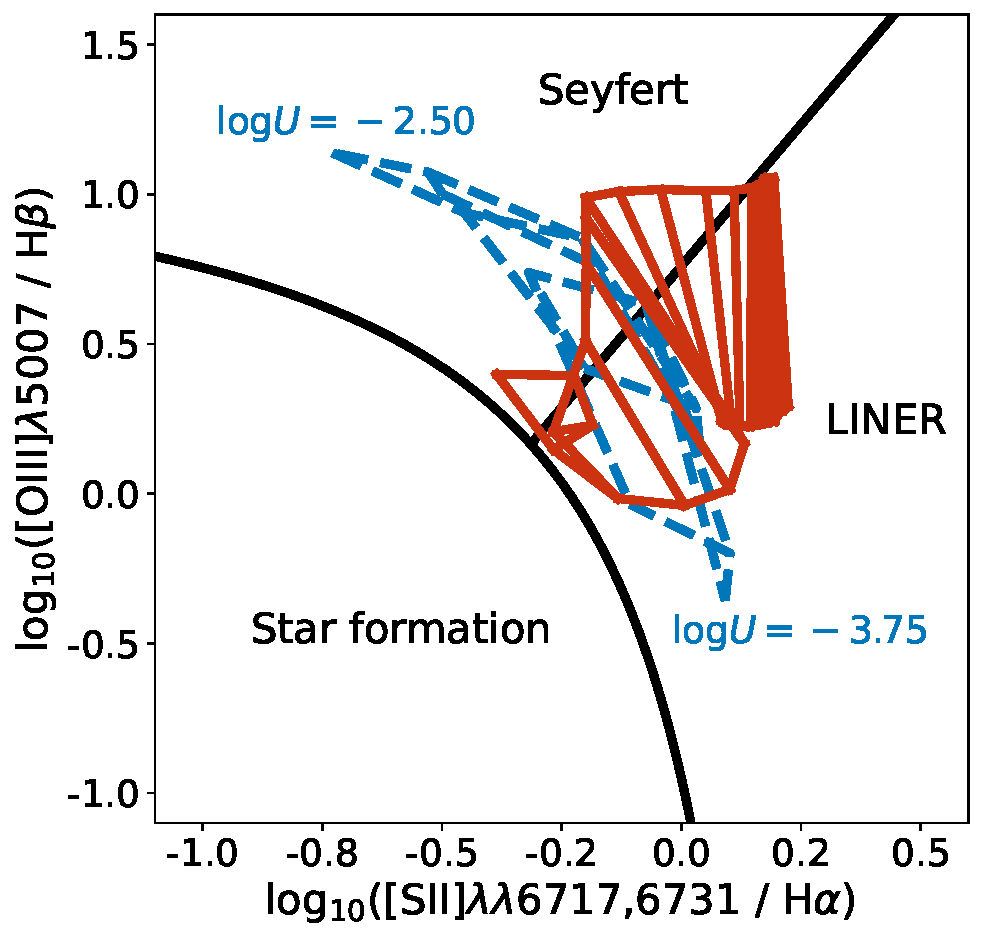
\includegraphics[width=0.75\linewidth]{figures/introduction/bpt_diagram_photo_shock_ionisation.pdf}
    \caption[{[SII]/H$\alpha$ vs [OIII]/H$\beta$ BPT \citep{Baldwin1981, Kewley2006} diagram with shock and photoionisation modelling.}]{[SII]/H$\alpha$ vs [OIII]/H$\beta$ BPT diagram \citep{Baldwin1981}, showing three empirically-defined regions \citep{Kewley2006} for Seyfert nuclei, star-forming regions, and LINERs, in addition to predictions of photoionisation (dashed blue grid) and pure shock-ionisation (solid red grid) modelling, which overlap significantly at the boundary between the Seyfert and LINER regions. The photoionisation models were generated using the \textsc{Cloudy} code (version C17.02: \citealt{Ferland2017}) for a radiation-bounded gas with varying ionisation parameter ($-3.75$\;\textless\;log$U$\;\textless\;$-2.50$; labelled) and electron density ($n_e=10^2,10^3,10^4$\;cm$^{-3}$), while the shock models are those generated using the \textsc{Mappings III} code by \citet{Allen2008} for shock velocities in the range 200\;\textless\;$v_\mathrm{shock}$\;\textless\;1000\;km\;s$^{-1}$ and magnetic parameters of $B/\sqrt{n}=2,10$\;$\mu$G\;cm$^{3/2}$.}
    \label{fig: introduction: outflows: acceleration_mechanisms: bpt_diagram_photo_shock_ionisation}
\end{figure}

To provide further information about the conditions of the warm-ionised gas, and to better discriminate between photo- and shock-ionisation, \citet{VillarMartin1999} created a diagnostic diagram plotting the [OIII](5007/4363) ratio against the He\;II$\lambda$4686/H$\beta$ ratio. The former ratio is dependent on the electron temperature of the emitting gas (shocked gas is expected to have higher temperatures: \citealt{Fosbury1978}), while the latter probes the presence of matter-bounded clouds, which may have similar temperatures to shocked gas \citep{Binette1996}. Therefore, the regions of photo- and shock-ionisation are more cleanly separated than in the typical BPT diagnostics. However, this diagram still only traces a single phase --- the warm-ionised gas.

Near-infrared (NIR) studies have revealed relations between emission-line flux ratios that may be powerful ionisation/excitation diagnostics of the warm ionised \textit{and} warm molecular phases. \citet{Larkin1998} first discovered a correlation between the NIR [FeII]$\lambda$12567/Pa$\beta$ and H$_2$(1--0)S(1)\;2.212\;$\mu$m/Br$\gamma$ ratios in LINERs, with higher values being associated with objects with known shocks. This correlation was subsequently confirmed, and empirical limits for different regions were refined using samples of star-forming galaxies (SFGs), LINERs, luminous infrared galaxies (LIRGs; L$_\mathrm{IR}$\;\textgreater\;$3.8\times10^{44}$\;erg\;s$^{-1}$: \citealt{Sanders1996}), and Seyfert galaxies, allowing the use of these ratios as a diagnostic diagram \citep{Rodriguez-Ardila2005, Riffel2013a, Colina2015, Riffel2021}. Since the H$_2$(1--0)S(1)\;2.212\;$\mu$m line arises from the warm molecular phase (Table\;\ref{tab: introduction: outflows: energetics: multi-phase: outflow_phases}), the H$_2$(1--0)S(1)\;2.212\;$\mu$m/Br$\gamma$ ratio axis of this diagram may be interpreted as tracing the relative excitation of the warm-molecular gas, with higher values associated with shock-excited gas. The physical interpretation for higher values of the [FeII]$\lambda$12567/Pa$\beta$ ratio is that iron is thought to be locked up in dust grains relatively easily: since dust grains are destroyed in shocks, iron is expected to be more abundant (and the [FeII]$\lambda$12567/Pa$\beta$ ratio therefore higher) post-shock. Support for this idea is provided by observed enhancements in the [FeII]$\lambda$12567/[PII]$\lambda$11886 ratio: phosphorus is less easily locked up in dust grains, and therefore it is notable that \citet{Riffel2013b} found enhanced values of [FeII]$\lambda$12567/[PII]$\lambda$11886 at the location of enhanced [FeII]$\lambda$12567/Pa$\beta$ along the radio axis of Seyfert\;1 galaxy Markarian (Mrk)\;79. This indicates that the [FeII]$\lambda$12567/Pa$\beta$ ratio is itself sensitive to the presence of shocks, which is further supported by an observed correlation between [FeII]$\lambda$12567/Pa$\beta$ and emission-line width (indicating that more-kinematically-disturbed gas has passed through a shock: \citealt{Riffel2021}).

\subsubsection{Photo- and shock-ionisation modelling}
\label{section: introduction: outflows: acceleration_mechanisms: modelling}

Producing diagnostic diagrams with accurate regions for different ionisation mechanisms requires predicted emission-line-flux ratios from ionisation models of different types, principally photo- and shock-ionisation. However, there are important complexities and variations of these two main mechanisms that need to be carefully considered. For photoionisation models, there are two general ionised-cloud geometries: radiation-bounded and matter-bounded. In the former case, the ionised region of a given gas cloud (and therefore the ionisation front) is located well within the boundaries of the cloud itself, so that there exists a stratification consisting of fully-ionised, partially-ionised, and neutral-atomic gas within the cloud. For matter-bounded geometry, the outer boundary of the ionised region is the physical boundary of the cloud itself; the cloud is (almost) completely ionised. Therefore, compared to the radiation-bounded case, higher-ionisation emission lines are much stronger relative to lower-ionisation emission lines. Regarding shock-ionisation, modern models often consider two distinct ionisation sources: collisional ionisation as material passes through the shock, and the photoionisation of pre-shock gas by the approaching shock front (commonly referred to as the `precursor' ionisation component). The relative ionisation contribution of these two components is often unclear, and depends strongly on the properties of the ISM and the shock(s), hence it is common practice to produce distinct regions for pure-shock (referred to throughout this thesis as solely `shock') and precursor ionisation.

For gas densities that are typical for the NLR ($n\ll10^{10}$\;cm$^{-3}$), the photoionisation code \textsc{CLOUDY} \citep{Ferland2017} can readily produce radiation-bounded models that predict accurate line ratios for a range of gas and photoionising-source properties. However, generating photoionisation models with a mix of matter- and radiation-bounded clouds (required to determine relative contributions to line fluxes) with \textsc{CLOUDY} is complex --- a good supplement is to use the photoionisation models presented by \citet{Binette1996}, which provide the predicted fluxes of many key diagnostic lines for different relative fractions of radiation- and matter-bounded clouds. Used together, \textsc{CLOUDY} and the models of \citet{Binette1996} can produce diagnostic-diagram photoionisation regions for both photoionised-cloud geometries.

\citet{Allen2008} used the MAPPINGS III ionisation code to produce a suite of emission-line-flux predictions for both pure-shock and precursor ionisation for varying ISM and shock parameters. However, a major drawback of these models is that they only consider one spatial-dimension, which does not properly allow for additional thermal instabilities and potential secondary shocks (see discussion in \citealt{Allen2008}). While this could potentially affect simulated absolute line fluxes, the predictions of these models are still sufficiently accurate for placing the regions of expected shock-ionisation on diagnostic diagrams.

In general, a major problem with using photo- and shock-ionisation models to predict line ratios for the use in diagnostic diagrams is that the predicted ratios depend strongly on the properties of the ISM (e.g. gas densities and metallicities), photoionising sources (ionisation parameters, spectral indicies), and shocks (e.g. shock speeds and magnetic fields). Therefore, constraining these parameters where possible is essential, either via direct estimation using other methods (e.g. ionisation parameters from the technique presented by \citealt{Baron2019a} and electron densities from the transauroral-line ratio technique of \citealt{Holt2011}) or assuming a range of reasonable values (such as magnetic parameters that are characteristic of the ISM: \citealt{Allen2008}; see Figure \ref{fig: introduction: outflows: acceleration_mechanisms: bpt_diagram_photo_shock_ionisation}).

\subsubsection{Uncertainties regarding outflow acceleration mechanisms}
\label{section: introduction: outflows: accleration_mechanisms: conclusions}

Overall, AGN-driven-outflow acceleration mechanisms are poorly understood, and are a matter of significant debate: there are many contradictions and claims of different mechanisms being dominant, even for individual objects (e.g. for NGC\;1068: \citealt{Axon1998, Crenshaw2000_N1068, Das2005, Fischer2017, May2017,  Revalski2021, Meena2023}). Principally, this is because the relationship between acceleration mechanisms and outflow ionisation/excitation is not clear, nor is the connection between NLR gas properties and radio structures.

The kiloparsec-scale linear double or triple radio structures seen in Seyfert galaxies (e.g. Figure\;\ref{fig: introduction: historical_context: nlr_studies: wilson1982_ngc1068_15ghz}: \citealt{Wilson1982}; \citealt{Wilson1980, Pedlar1983, Pedlar1984, Ulvestad1984}) are likely tracing synchrotron emission produced by shocks or radio plasma \citep{Wilson1980, Ulvestad1984}. It is commonly argued that, based on the morphologies of these structures and the presence of small-scale radio knots close to the nucleus, these structures represent AGN jets propagating into the ISM (e.g. \citealt{Wilson1982, Stanghellini2005, Rosario2010b, Riffel2013b, Jarvis2019, Williams2017, Girdhar2022}). In contrast, other authors have argued that the synchrotron emission is produced by shocks that are induced when radiatively-driven winds (i.e. such as those invoked in modelling by \citealt{Hopkins2010}; see Section\;\ref{section: introduction: outflows: accleration_mechanisms: radiation}) impact the ISM, launching kpc-scale outflows in the process (\citealt{Fischer2019}; see also \citealt{Fischer2023}).

Regardless of the source of the shocks, it is not clear how well ionisation/excitation mechanisms correspond to radiative or shock-acceleration. While line ratios consistent with shock-ionisation/excitation indicate that the emitting material has passed through (and thus been accelerated by) a shock, photoionised gas does not necessarily imply radiative acceleration: it is possible that the material passed through a shock, cooled, and then was re-ionised by radiation from the AGN. 

Determining precise diagnostics of outflow acceleration, ionisation/excitation, and the links between these is therefore essential: simulations of different mechanisms are now able to predict specific outflow properties (e.g. \citealt{Richings2021, Meenakshi2022a, Meenakshi2022b}; see \citealt{Krause2023} for a review), allowing detailed observational studies to directly test their assumptions regarding the underlying physics. Moreover, a complete understanding of outflow acceleration is needed to inform the sub-grid\footnote{Many cosmological simulations divide the three-dimensional volume that they consider into a grid of cells; the spatial size of the cells effectively sets the spatial resolution of the simulation. `Sub-grid' refers to processes in such simulations that take place on scales smaller than the cell size.} physics of cosmological simulations, for which AGN feedback in the form of outflows is required to reproduce observed galaxy properties \citep{Schaye2015, Dubois2016, Dave2019, Zinger2020}.

\subsection{Taxonomy of AGN}
\label{section: introduction: outflows: taxonomy_of_agn}

Active galaxies of different types provide distinct, useful laboratories to investigate outflow properties and acceleration mechanisms. Here, I briefly summarise AGN classification (see \citealt{Netzer2015} and \citealt{Tadhunter2008, Tadhunter2016} for reviews) and define the types of galaxies and AGN that are considered in this thesis. 

\subsubsection{Optical classifications}
\label{section: introduction: outflows: taxonomy_of_agn: seyferts_and_quasars}

The term `Seyfert' galaxy was originally used to refer to nearby active galaxies with nuclei that showed optical spectral features characteristic of planetary nebulae, indicating high ionisation. As described in Section\;\ref{section: introduction: historical_context: early_studies}, the systematic study of these objects began with the seminal work of \citet{Seyfert1943}; subsequent studies often adopted various definitions for the term based on properties such as optical and radio luminosities \citep{Wilson1980}, emission-line ratios \citep{Baldwin1981}, and line widths \citep{Whittle1992a}. In this thesis, I define Seyfert galaxies\footnote{Some classical Seyfert galaxies --- notably NGC\;1068, which is considered in Chapter\;\ref{chapter: stis_seyferts} --- have bolometric luminosities that are close to (and potentially above) the limit used in this definition.} to be galaxies with nuclei that present line ratios that are consistent with the AGN/Seyfert regions of the BPT diagrams (to separate them from LINERs and star-forming/HII galaxies: \citealt{Baldwin1981, Kewley2006}), line widths of FWHM\;\textgreater\;200\;km\;s$^{-1}$, and have bolometric luminosities of $L_\mathrm{bol}$\;\textless\;10$^{45}$\;erg\;s$^{-1}$ (to distinguish them from quasars).

Although quasars were originally considered to be a distinct class of object (Section\;\ref{section: introduction: historical_context: radio_astronomy}), it is now accepted that they are intrinsically the same phenomenon as Seyfert galaxies, only with higher optical luminosities; there likely exists a continuous scale of bolometric luminosity between the two classes. Therefore, here I define quasars (QSOs) to be objects with the same properties as Seyfert galaxies, except with higher bolometric luminosities ($L_\mathrm{bol}$\;\textgreater\;10$^{45}$\;erg\;s$^{-1}$).

As discussed in Section\;\ref{section: introduction: historical_context: nlr_studies: unified scheme}, by the end of 1960s, it was appreciated that Seyfert galaxies present a dichotomy in the widths of their forbidden and permitted lines. Therefore, they were sub-classified into Seyfert\;1s, which present narrow (200\;\textless\;FWHM\;\textless\;1000\;km\;s$^{-1}$) forbidden lines and broad (FWHM\;\textgreater\;1000\;km\;s$^{-1}$) permitted lines, and Seyfert\;2s, which present narrow forbidden and permitted lines \citep{Khachikian1971}. With the recognition that Seyfert galaxies and quasars are likely the same phenomenon, these classifications were extended to quasars (QSO1s and QSO2s), and later generalised to all AGN (Type\;1 and Type\;2). In the unified scheme of AGN (Figure\;\ref{fig: introduction: historical_context: nlr_studies: unified_scheme}), Type\;1 and Type\;2 AGN of a given class are the same intrinsic phenomenon, only viewed along different lines of sight.

Seyfert galaxies and quasars --- as defined here --- provide different regimes for probing AGN feedback in the inner regions of galaxies ($r$\;\textless\;5\;kpc). Owing to their higher bolometric luminosities, quasars are perhaps expected to impart greater radiation pressure on NLR gas (and/or drive stronger radiatively-driven winds) than Seyfert galaxies, and therefore photoionisation and radiative outflow-acceleration may be dominant. In contrast, the lower bolometric luminosities of Seyfert galaxies may mean that potential optical tracers of jet-ISM interactions are not obscured by dominant photoionisation that results from the intense radiation of the central AGN, and, based on previous NLR studies (e.g. \citealt{Whittle1992a, Axon1998, Crenshaw2000_N1068, Das2007}), it may be expected that they are more likely to host a mixture of jet- and radiation-driven outflows.

Similar to the classification schemes for objects detected at optical wavelengths, the optical properties of radio galaxies (galaxies detected via their radio emission) are often separated into the Broad Line Radio Galaxy (BLRG; Type 1 AGN: \citealt{Osterbrock1976, Grandi1977}) and Narrow Line Radio Galaxy (NLRG; Type 2 AGN: \citealt{Costero1977}) subclasses. However, objects of these classifications (collectively known as Strong Line Radio Galaxies, or SLRGs: e.g. \citealt{RamosAlmeida2011}) form only a subset of the radio-galaxy population: a significant fraction of radio galaxies instead present weak optical emission lines (known as Weak Line Radio Galaxies, or WLRGs: \citealt{HineLongair1979, Best2012}). The SLRG and WLRG classes --- defined by the [OIII]$\lambda5007$ equivalent width (e.g. $\mathrm{EW}_\mathrm{[OIII]}$\;\textless\;10\;{\AA} for WLRGs: \citealt{Tadhunter1998}) --- have considerable (but not complete) overlap with the commonly-used classifications of High Excitation Radio Galaxies (HERGs: \citealt{Laing1994, Tadhunter1998, Best2012}; see discussion in \citealt{Tadhunter2016}) and Low Excitation Radio Galaxies (LERGs), respectively, which are defined based on measured emission-line ratios (e.g. \citealt{Buttiglione2010}).

Although not directly considered in this thesis, also of note is the LINER (Low Ionisation Nuclear Emission Region) classification \citep{Heckman1980}, comprising objects that display prominent low-ionisation lines (e.g. [OI], [OII], [NII], [SII]), but weak high-ionisation lines (e.g. [OIII]), in their spectra. It is not clear whether LINERs are a true class of AGN or if the observed ionisation is (at least in part) due to stellar radiation \citep{CidFernandes2011, Singh2013, Coldwell2018, Frederick2019}. As discussed earlier, emission-line widths and diagnostic diagrams making use of multiple emission-line ratios (such as the BPT diagnostics: e.g. Figure\;\ref{fig: introduction: outflows: acceleration_mechanisms: bpt_diagram_photo_shock_ionisation}) can be used to distinguish between bonafide AGN and non-AGN LINERs.


\subsubsection{Radio classifications}
\label{section: introduction: outflows: taxonomy_of_agn: css_and_gps_sources}

As a result of radio astronomy playing a prominent role in the development of AGN as an important field of modern astrophysics, there are also classification schemes based on object properties at radio frequencies (see \citealt{Tadhunter2016} for a comprehensive review). The earliest AGN detected and identified at radio wavelengths are luminous radio sources ($L_\mathrm{1.4\;GHz}$\;\textgreater\;$10^{25}$\;W\;Hz$^{-1}$), and often have radio structures that extend far beyond their host galaxies (e.g. $r_\mathrm{jet}\sim60$\;kpc for Cygnus\;A: \citealt{Carilli1991}); the most-commonly-used radio classifications are the Fanaroff-Riley classes \citep{Fanaroff1974}, which separate such radio morphologies into `edge-darkened' (FR\;I) and `edge-brightened' (FR\;II; e.g. Cygnus\;A).

However, there also exist classes of luminous radio AGN that present complex radio structures on sub-galactic scales, the most important of which are compact steep spectrum (CSS) and gigahertz peaked spectrum (GPS) sources  (see \citealt{ODea1998} and \citealt{ODea2021} for reviews). The radio structures of CSS sources typically have radial extents of $r$\;\textless\;15\;kpc and have steep ($\alpha$\;\textless\;$-0.5$)\footnote{Radio continua are typically characterised by spectral indices ($\alpha$), defined as $F_\mathrm{\nu}\propto\nu^\alpha$, where $F_\mathrm{\nu}$ is the monochromatic flux density at the frequency $\nu$.} radio spectra, while those of GPS sources are typically sub-kpc-scale and peak at gigahertz frequencies \citep{Kellermann1981, ODea1998, Callingham2015}. The morphologies of these sources are often double or triple, similar to those seen in classical Seyfert galaxies (Figure\;\ref{fig: introduction: historical_context: nlr_studies: wilson1982_ngc1068_15ghz}: \citealt{Wilson1982}) and in radio galaxies on larger scales (FRII), indicative of jets. The compactness of the radio structures of CSS/GPS sources may be explainable if their jets are young and/or are being confined by the dense ISM \citep{Bicknell1997, Stanghellini2005, ODea2021}, from which they eventually grow and subsequently evolve into larger-scale radio galaxies \citep{Stanghellini2005, Morganti2007, Kukreti2023}. This process would be expected to entail prominent jet-ISM interactions, and thus CSS/GPS sources host powerful outflows (e.g. \citealt{Holt2008, Holt2011, Santoro2020}).

\subsubsection{Ultra luminous infrared galaxies}
\label{section: introduction: outflows: taxonomy_of_agn: ulirgs}

Finally, although not strictly a class of AGN, ultra luminous infrared galaxies (ULIRGs) are an important class of galaxy for studies of AGN-driven outflows. These are defined as galaxies with infrared luminosities above 10$^{12}$ solar luminosities ($L_\mathrm{5-500\;\mu{m}}$\;\textgreater\;$3.8\times10^{45}$\;erg\;s$^{-1}$: \citealt{Sanders1996}). Almost all (\textgreater\;90\;per\;cent: \citealt{Veilleux2002}) ULIRGs show morphological evidence for strong tidal interactions, and so it is thought that they represent the peaks of gas-rich major mergers. Therefore, they are considered to be the most rapidly evolving galaxies in the local Universe, and thus represent the situation modelled in hydrodynamical simulations which predict AGN triggered in mergers that launch galaxy-wide outflows \citep{DiMatteo2005, Springel2005, Hopkins2008, Johansson2009}. Indeed, a significant fraction ($\sim$40--70\;per\;cent: \citealt{Kim1998, Veilleux2002, Nardini2010, AlonsoHerrero2012}) of ULIRGs host AGN. For these reasons, they are expected to host prominent outflows, which have been now observed in a range of gas phases (e.g. \citealt{Zaurin2013, Spence2018, Rose2018, Tadhunter2019, Lamperti2022}).

\section{Outstanding problems addressed by this thesis}
\label{section: introduction: outstanding problems}

Overall, while significant progress has been made in understanding AGN-driven outflows over the past twenty-five years, their true properties, natures, and role in galaxy evolution are still largely unclear. Key outstanding questions include the following. \\

\begin{itemize}
    \item Which outflow phase(s) is dominant in terms of mass and kinetic power, and how are the different phases physically linked?
    \item What are the true electron densities of the warm ionised outflow phase, and what is the impact on derived outflow kinetic powers?
    \item Are AGN-driven outflows truly galaxy-wide, as predicted by simulations of galaxy evolution?
    \item How are outflows accelerated by AGN, and what is the relationship between outflow excitation/ionisation mechanisms and acceleration mechanisms? \\
\end{itemize}

To address these important questions, in this thesis I present detailed studies of four nearby active galaxies, three of which are classified as Seyfert galaxies and the other a ULIRG/QSO/GPS source. The studies make use of deep, high-spatial-resolution, multi-wavelength observations that trace different gas phases --- in addition to developing and utilising precise outflow diagnostic techniques --- to robustly quantify outflow properties and interpret their impact on the host galaxies. The observations and analyses are presented in the chapters of this thesis as follows. \\

\begin{itemize}
    \item In Chapter\;\ref{chapter: xshooter_ic5063}, I present a study based on high-spatial-resolution, wide-wavelength-coverage long-slit VLT/Xshooter spectroscopy of the kpc-scale radio structure of the nearby Sey\;2 galaxy IC\;5063, which is known to host prominent jet-driven outflows. The principal aims of this analysis were to determine robust spatially-resolved electron densities using the transauroral-line method (for the first time), verify the use of this method in studies of AGN-driven outflows, and place the resulting precise warm-ionised outflow properties in a multi-phase context using the wealth of previous observations of this object, therefore allowing an investigation into the relative importance of the various outflow phases and the physical link(s) between them. The work presented in this chapter is based on the 1st first-author publication of my PhD \citep{Holden2023}.
    \item Extending this analysis to other nearby active galaxies, in Chapter\;\ref{chapter: stis_seyferts} I analyse HST/STIS spectroscopy of the inner few-hundred parsecs of the prototypical Seyfert galaxies NGC\;1068 and NGC\;4151. Using the transauroral-line technique, this data is used to measure spatially-resolved electron densities for these two objects, which are then compared to the results of previous detailed photoionisation modelling to further verify this method. Moreover, the high-spatial-resolution STIS observations allow for the ionisation conditions of the gas to be determined; combining this with information regarding the radio structures in the NLRs, the link between ionisation and acceleration mechanisms is investigated, permitting a detailed study into the launching mechanism of the outflows. This analysis and subsequent results were first presented in the 2nd first-author publication of my PhD \citep{HoldenTadhunter2023}.
    \item Chapter\;\ref{chapter: alma_f13451_1232} presents an ALMA CO(1--0) study of the cold-molecular gas in the inner few kiloparsecs of the primary nucleus of the ULIRG/QSO/GPS source F13451+1232, an object which directly represents the situation considered in models of galaxy evolution. While compact ($r$\;\textless\;100\;pc) outflows have been detected in this object in various phases previously, there has not yet been a robust detection of molecular outflows --- a potentially crucial phase. The ALMA CO(1--0) observations are used to search for molecular outflows, with the aim of completing the multi-phase information and thus allowing for the relative importance of the various phases to be established for an object of higher radio and bolometric luminosity than the Seyfert galaxies considered in prior chapters. Furthermore, the high spatial resolution of the ALMA observations allows for the spatial extents of molecular outflows to be determined (thus addressing a prediction of galaxy evolution models), and by combining them with archival VLBI observations, the outflow acceleration mechanism(s) are investigated. This chapter is based on the third 1st-author publication of my PhD \citep{Holden2024}.
    \item The techniques and analyses used in the previous three chapters are sensitive to relatively dense ($n_e$\;\textgreater\;$10^{3}$\;cm$^{-3}$) gas in the central kiloparsecs of galaxies. Therefore, to directly verify the true spatial extents of the warm ionised outflow phase, Chapter\;\ref{chapter: muse_f13451_1232} presents a VLT/MUSE IFU study of F13451+1232 on galaxy-scales ($r$\;\textgreater\;5\;kpc) --- an object which, according to models of galaxy evolution, would be expected to host prominent galaxy-wide outflows. Unlike previous, similar ground-based IFU studies of outflows in local AGN, the analysis of this chapter carefully accounts for the beam-smearing effects of atmospheric seeing, and quantifies its effect on key outflow properties including spatial extents, kinematics, mass outflow rates, and kinetic powers.
    \item Finally, in Chapter\;\ref{chapter: conclusions_and_future_work} I summarise the results of these chapters and present the conclusions of this thesis. Moreover, I discuss future work that can be undertaken in this field, in addition to important considerations that are required for further significant progress to be made in understanding the nature of AGN-driven outflows and their role in galaxy evolution.
\end{itemize}


\newpage
\thispagestyle{plain}
~\newpage

\chapter{Jet-driven warm gas outflows in the Seyfert 2 galaxy IC 5063}
\chaptermark{Warm gas outflows in IC 5063}
\label{chapter: xshooter_ic5063}

\vspace*{2cm}
\vbox{\large``Born under a black sun, \\
malignant solar tides. \\
Infinite aeons, merge! Collide! \\
Spiralling down. \\

\noindent
Celestial dagger, \\
terminate galaxies, \\
pierce through the heart of the void, \\
storm heaven, \\
ride, divide and conquer.''\\

--- \href{https://wode.bandcamp.com/album/servants-of-the-countercosmos}{Wode, \textit{Celestial Dagger}}}
\newpage
\noindent
\section*{Chapter declaration}
\addcontentsline{toc}{section}{\numberline{}Chapter declaration}
The data, analysis, results, and discussion presented in this chapter were reported in my first-author publication ``Precise physical conditions for the warm gas outflows in the nearby active galaxy IC 5063'' \citep{Holden2023}. The content of this chapter is based on that publication, which has been adapted into a suitable format for this thesis; all work is my own, except where clearly stated.

\newpage

\section{Chapter introduction}
\label{section: xshooter_ic5063: introduction}

% \subsection{IC\;5063}
% \label{section: xshooter_ic5063: introduction: ic5063}

An important object for investigating multi-phase AGN-driven outflows is IC\;5063: a nearby ($z=0.01131$) early-type galaxy with a Seyfert\;2 nucleus \citep{Danziger1981, Inglis1993}. The galaxy hosts a gaseous disk that is detected out to a radius of $r\sim28$\;kpc in HI 21\;cm emission, is associated with prominent dust lanes, and may be the result of a merger \citep{Morganti1998}. The inner parts of this disk (within a few kiloparsecs of the nucleus) are also detected in cold \citep{Morganti2015} and warm H$_2$ \citep{Tadhunter2014} molecular gas emission. In addition, [OIII] emission lines from warm-ionised gas are detected in HST imaging along the edges of the dust lane to a radius of $\sim$10\;kpc \citep{Morganti1998}.  Importantly, IC\;5063 has a radio luminosity at the upper end of the range for Seyfert galaxies ($L_\mathrm{1.4\;GHz}=3\times10^{23}$\;W\;Hz$^{-1}$), and the radio emission is concentrated in a triple-structure that is parallel to the dust lanes, consisting of a nucleus and two radio lobes $\sim$2\;arcsec ($\sim$0.5\;kpc) on either side of the nucleus to the southeast (SE) and northwest (NW) (Figure\;\ref{fig: introduction: outflows: energetics: multi-phase: morganti2015_ic5063_multiphase}). 

As expected for an object of its 1.4\;GHz luminosity (Section\;\ref{section: introduction: outflows: accleration_mechanisms: jet_driven_outflows}; \citealt{Whittle1988, Whittle1992c, Mullaney2013}), past observations of IC\;5063 have revealed fast (\mbox{$v$\;\textgreater\;700\;km\;s$^{-1}$}) outflows spatially associated with the NW radio lobe across a range of gas phases: warm ionised \citep{Morganti2007, Sharp2010, Congiu2017, Venturi2021}; neutral \citep{Morganti1998, Oosterloo2000}; warm molecular \citep{Tadhunter2014}, and cold molecular \citep{Morganti2013_IC5063, Morganti2015, Dasyra2016, Oosterloo2017}. In addition, IC\;5063 has been the target of X-ray observations tracing hot ionised gas, which presents a biconical morphology with an axis similar to that of the radio structure \citep{Vignali1997, Tazaki2011, Travascio2021}.

IC\;5063 is unusual in the sense that its radio structure lies in the plane of its disk \citep{Morganti1998, Oosterloo2000, Morganti2015, Mukherjee2018}. Considering that the outflows in the galaxy are spatially associated with the bright radio features, particularly at the NW radio lobe, it is thought that jet-ISM interactions are the main outflow acceleration mechanism, with these interactions being particularly strong due to jets propagating in the dense ISM of the disk \citep{Tadhunter2014, Morganti2015}. Hydrodynamic simulations by \citet{Mukherjee2018} explain the gas kinematics in IC\;5063 by assuming that a relatively-low-power jet (P$_\mathrm{jet}=10^{44-45}$\;erg\;s$^{-1}$) percolates through the path of least resistance in the disk. As it does so, jet-ISM interactions accelerate gas perpendicular to the jet direction. This is supported by observations of a giant low-ionisation loop \citep{Maksym2020} and enhanced [OIII] velocity width \citep{Venturi2021} around the radio structure.

The properties described above make IC\;5063 an ideal case study for addressing three of the main outstanding questions that are the focus of this thesis. First, its close proximity to Earth allows its NLR and outflows to be spatially resolved, permitting comparisons (and verification) of different electron-density diagnostics (particularly the transauroral-line method) --- crucial for determining robust outflow kinetic powers for the warm ionised phase. Second, the jets propagating directly into the galaxy's disk are expected to produce prominent jet-ISM interactions --- spatially-resolved observations of these interactions may reveal how the outflows are accelerated. Finally, the extensive previous multi-wavelength observations allow for results to be placed into a wider, multi-phase context, directly constraining the relative energetic contributions of the different phases and permitting an investigation into the physical link between them. For these reasons, IC\;5063 was chosen to be the target of deep observations with the Very Large Telescope's (VLT) Xshooter spectrograph in 2018.

Throughout this chapter, I assume a cosmology of $H_\mathrm{0} = 70$\;km\;s$^{-1}$\;Mpc$^{-1}$, $\Omega_\mathrm{m}=0.3$ and ${\Omega}_\mathrm{\lambda}=0.7$. At the redshift of IC\;5063 ($z=0.01131$; \citealt{Tadhunter2014}), this corresponds to a luminosity distance of $D_\mathrm{L}=48.9$\;Mpc and an angular scale of 0.231\;kpc/arcsec.

\section{Observations and data reduction}
\label{section: xshooter_ic5063: observations_and_data_reduction}

\subsection{Xshooter observations of IC 5063}
\label{section: xshooter_ic5063: observations_and_data_reduction: observations}

IC\;5063 was observed using VLT/Xshooter in service mode on the nights of the 13th and 16th June 2018 in four observing blocks (OBs) during photometric and dark sky conditions, as part of the ESO programme 0101.B0409(A) (PI: Tadhunter). The observations were performed in long-slit mode (slit length = 11\;arcsec), with slit widths of 1.3\;arcsec for the UVB arm (wavelength range: 3200--5600\;\AA) and 1.2\;arcsec for the VIS (5500--10200\;\AA) and NIR (10200--24750\;\AA) arms. The slit was aligned along the galaxy's radio axis ($\mathrm{PA}=115^{\circ}$), meaning that the radio hotspots ($\sim$4\;arcsec separation) were contained in the 11\;arcsec slit length (see Figure\;\ref{fig: observations_and_data_reduction: xshooter_ic_5063: observations: ic5063_hst_17ghz}). The data has a pixel scale of 0.16\;arcsec/pixel for the UVB and VIS arms and 0.21\;arcsec/pixel for the NIR arm. Separate sky exposures were taken by nodding off the target object with a 30-arcsecond spatial offset and using an ABBA observing pattern --- this facilitated accurate sky subtraction during data reduction. Each observing block thus consisted of 6 exposures (3 on-object and 3 on-sky), with a total integrated object exposure time of 5400\;s. In addition, standard calibration files (e.g. bias frames, dark frames and standard star observations) were provided along with the science data for use in data reduction.

\begin{figure}
    \includegraphics[width=\linewidth]{figures/observations_and_data_reduction/ic5063_hst_17ghz.png}
    \caption[VLT/Xshooter slit position used for the observations the Seyfert\;2 galaxy IC\;5063, overlaid on optical and 17\;GHz radio continuum imaging.]{Archival HST/WFPC2 F606W optical image of the central $\sim$3\;kpc of IC\;5063 (Cycle 4; SNAP:5479; PI Malkan), in addition to ATCA 17\;GHz radio imaging (\citealt{Morganti2007}; shown as white contours). The slit is overlaid in black, with the borders of each aperture along the slit (Section\;\ref{section: xshooter_ic_5063: observations_and_data_reduction: apertures}; Figure\;\ref{fig: xshooter_ic5063: apertures}) shown and labelled in blue. The northwest (NW) and southeast (SE) radio lobes are labelled, along with the nucleus. Note that the F606W filter admits strong [OIII] and H$\mathrm{\alpha}$+[NII] emission lines, as well as continuum emission. In this negative image, the inner part of a large-scale dust lane can be seen as the lighter-toned filamentary structures to the north of the nucleus, whereas the inner emission-line structures appear as the darker grey or black features close to the nucleus. \textit{Image credit: the alignment of the HST/WFPC2 optical image and the 17\;GHz radio image was performed by Raffaella Morganti and Tom Oosterloo; the remaining preparation of the figure was done by myself.}}
    \label{fig: observations_and_data_reduction: xshooter_ic_5063: observations: ic5063_hst_17ghz}
\end{figure}

In order to determine the instrumental broadening of the Xshooter observations, Gaussian profiles were fitted to the Galactic NaID absorption lines at 5890\;{\AA} and 5896\;{\AA}. Since the gas responsible for this absorption is quiescent (i.e non-outflowing) within the Milky Way, any broadening of these lines will be due entirely to the instrumental setup. From the galactic NaID lines, an instrumental width of FWHM$_\mathrm{inst}$ = 0.825$\pm$0.016\;{\AA} was measured, corresponding to a velocity resolution of 42.0$\pm$0.8\;km\;s$^{-1}$ at 5900\;\AA. I note that I did not make use of the instrument's calibration lamps when measuring the instrumental broadening to avoid potential inaccuracies arising from telescope and instrument flexture at different pointings; residual sky lines were not used as they were (first-order) subtracted during the pipeline data-reduction process.

\subsection{Seeing estimates}
\label{section: xshooter_ic_5063: observations_and_data_reduction: seeing}

Estimates of the seeing during the four observing blocks were made by fitting one-dimensional Gaussian profiles\footnote{While atmospheric seeing profiles are accurately described by a Moffat distribution \citep{Moffat1969}, a Gaussian profile is a sufficient approximation for the purposes of this chapter.} to the spatial slices of stars in the acquisition images taken with the Sloan r' filter for each observing block. The width of each spatial slice was 1.2\;arcsec, taken to match the Xshooter slit widths (and thus provide a robust representation of the seeing expected for the longslit spectra). Seeing estimates were also taken from the Paranal DIMM (Differential Image Motion Monitor)\footnote{DIMM seeing values were queried from \url{http://archive.eso.org/wdb/wdb/asm/dimm_paranal/form}} during the four observing blocks, as measured near zenith with a filter centred on $\sim$5000\;\AA. Seeing estimates measured from the acquisition images and the DIMM are given in Table\;\ref{tab: observations_and_data_reduction: xshooter_ic_5063: seeing: seeing}.

\begin{table}
    \centering
    {\renewcommand{\arraystretch}{2}
    \setlength{\tabcolsep}{20pt}
    \begin{tabular}{ccc}
    Observing Block & {Max DIMM (arcsec)} & Acq. Image (arcsec) \\ \hline
    1               & 0.83                                                         & 2.08$\pm$0.03                                                  \\
    2               & 1.06                                                         & 0.93$\pm$0.01                                           \\
    3               & 0.69                                                         & 0.93$\pm$0.01                                               \\
    4               & 0.74                                                         & 0.72$\pm$0.01                                              
    \end{tabular}
    }
    \caption[Seeing estimates for the VLT/Xshooter observations of IC\;5063.]{Seeing estimates for each observing block of the VLT/Xshooter observations of IC\;5063, taken on the nights of the 13th (Block 1) and 16th (blocks 2, 3 and 4) of June 2018. `Max DIMM' is the maximum seeing recorded by the VLT observatory DIMM during the time frame of a given observing block, and `Acq. Image' is the seeing measured by fitting one-dimensional Gaussian profiles to 1.2\;arcsecond wide spatial slices centred on stars in the r$^\prime$-band acquisition images.}
    \label{tab: observations_and_data_reduction: xshooter_ic_5063: seeing: seeing}
\end{table}

\subsection{Reduction of the Xshooter data}
\label{section: xshooter_ic_5063: observations_and_data_reduction: data_reduction}

The European Southern Observatory's (ESO) pipeline for Xshooter data reduction, \textsc{ESOReflex} (version 2.11.0; \citealt{Freudling2013}), was used for the initial stage of data reduction. Used with the calibration data provided by ESO, this produced a single two-dimensional, bias-subtracted, flat-fielded, order-merged, wavelength-calibrated, and flux-calibrated long-slit spectrum for each Xshooter arm (UVB, VIS, NIR) in each observing block, giving a total of 12 spectra (one for each arm per block).

Residual bad pixels, cosmic rays and other cosmetic defects in each spectrum were cleaned via interpolation using the \textsc{CLEAN} command from the \textsc{STARLINK FIGARO} package \citep{Currie2014}. A second-order correction was then applied to the NIR data to improve the night-sky-line subtraction --- this was done by taking the median of pixel rows near the edges of the slit (free of emission from the object) and subtracting the resulting spectrum from each pixel row of the entire slit.

Telluric correction of the VIS and NIR arm data to remove atmospheric absorption features was performed using ESO's \textsc{molecfit} software (version 1.5.9: \citealt{Smette2015, Kausch2015}). Atmospheric models were created using fits to key telluric absorption features which were then used to create synthetic transmission spectra for the VIS and NIR data. The two-dimensional spectra were subsequently telluric-corrected by dividing them by the corresponding transmission spectrum. After verifying that they were spatially aligned, the cleaned, second-order-corrected (for the NIR arm), and telluric-corrected two-dimensional spectra for the four observing blocks were then median-combined using \textsc{IRAF} \textsc{imcombine} \citep{Tody1986, Tody1993} into a single two-dimensional spectrum for each arm.

Extinction due to dust in the Milky Way galaxy was corrected using the Galactic extinction maps presented by \citet{Schlegel1998} and re-calibrated by \citet{Schlafly2011} (hereafter S98 and SF11, respectively). The mean colour excess value in the direction of IC\;5063 \mbox{($\mathrm{E(B}-\mathrm{V)}_\mathrm{mean} = 0.0526\pm0.0012$)} from these maps was found using the NASA/IPAC Infrared Science Archive reddening lookup tool\footnote{\url{https://irsa.ipac.caltech.edu/applications/DUST/}}; this value was used with the $R_\mathrm{v}=3.1$ extinction law presented by \citet{Cardelli1989} (hereafter CCM89) to correct for Galactic extinction. The spectra were then shifted into the rest frame of IC\;5063 using the \textsc{IRAF} \textsc{dopcor} command with the redshift of IC\;5063 ($z=0.01131$) measured by \citet{Tadhunter2014}.

\subsection{Aperture selection and extraction}
\label{section: xshooter_ic_5063: observations_and_data_reduction: apertures}

The VLT/Xshooter observations reveal highly disturbed gas kinematics and complex line profiles in the regions coincident with the radio structure (Figure\;\ref{fig: xshooter_ic5063: apertures}a), consistent with the observations presented by \citet{Morganti2007}. The reduced and merged two-dimensional spectra for the UVB and VIS Xshooter arms were divided into apertures (groupings of pixel rows) covering important features of the inner regions of IC\;5063. The apertures chosen for the UVB and VIS arms are shown in Figure\;\ref{fig: xshooter_ic5063: apertures}b, with Aperture 4 covering the nucleus, and apertures 3, 5, 6 and 7 covering distinct kinematic regions along the radio structure: Aperture 3 approximately covers the SE radio lobe, Aperture 5 covers a region of disturbed emission-line kinematics between the nucleus and the maximum extent of the NW lobe, and apertures 6 and 7 cover the NW radio lobe. Once the apertures were selected, the same pixel rows in both the UVB and VIS data were extracted and added to produce two one-dimensional spectra for each aperture (one UVB and one VIS); flux uncertainties were extracted and added in quadrature. Before extraction, Gaussian fitting of continua spatial-flux distributions in spectral regions that were free of line features at similar wavelengths in both the UVB and VIS arms was performed to ensure that the spectra in the two arms were closely spatially aligned. Due to slight differences in flux calibration, a small ($\sim$5\;per cent) correction was applied to the fluxes of the VIS data for each extracted aperture to make them consistent with the corresponding UVB aperture. This was done by measuring the average flux between 5440--5500\;{\AA} for the UVB arm and 5600--5660\;{\AA} for the VIS arm (chosen to avoid noise at the edges of the detectors)--- the ratio of these average fluxes was then used as a correction factor to match the flux scales across both arms. 

\begin{figure*}[!t]
	\includegraphics[width=\linewidth]{figures/xshooter_ic5063/apertures.png}
	\caption[Two-dimensional long-slit spectra along the radio axis of IC\;5063, with the positions of extracted apertures overlaid.]{\textbf{a)}: Two-dimensional spectrum of the H$\mathrm{\alpha}$+[NII] emission lines at $\sim$6560\;{\AA} in the VIS arm of the Xshooter data of IC\;5063, showing the line profiles in the inner regions of the galaxy. The spectral axis is horizontal and the spatial axis is vertical; the velocity and spatial scales are shown as a labelled green axis. The centroids of the radio lobes --- measured from 24.8\;GHz radio continuum imaging presented by \citet{Morganti2007} --- are shown as yellow dashed lines, and each lobe is labelled. \textbf{b)}: The same as in a), but with apertures selected for the UVB and VIS arms marked with white dashed lines and labelled as `1-8' on the left; the spatial width of each aperture in arcseconds is given on the right. Note that the H$\mathrm{\alpha}$+[NII] blend is shown here for presentation purposes, as it clearly demonstrates the emission-line structure of forbidden ([NII]) and permitted (H$\alpha$) species.}
	\label{fig: xshooter_ic5063: apertures}
\end{figure*}

Finally, the extracted and corrected UVB and VIS one-dimensional spectra were combined to produce a single one-dimensional spectrum for each aperture, covering the full wavelength range of both arms. During this process, the spectra for both arms were resampled to a common wavelength grid with steps of $\Delta\lambda$ = 1{\;\AA} using the \textsc{SpectRes} \citep{Carnall2017}, \textsc{specutils} \citep{Earl2021} and \textsc{Astropy} \citep{AstropyCollaboration2013, AstropyCollaboration2018} \textsc{Python} packages. $\Delta\lambda = 1${\;\AA} was chosen for the resampling because this was the smallest wavelength step allowed by the base stellar templates used in the stellar continuum modelling (described in Section\;\ref{section: xshooter_ic_5063: observations_and_data_reduction: starlight}). 

Because of the different spatial pixel scale of Xshooter's NIR arm relative to its UVB and VIS arms, the NIR data was considered separately. Apertures for the NIR data were derived from the UVB+VIS apertures by first fitting two Gaussian profiles to a spatial slice of the continuum near the [OIII]$\lambda\lambda$5007,4959 doublet and taking the centroid of the narrowest to be the position of the continuum peak along the slit --- the distances from the centre of each UVB+VIS aperture to this continuum peak were then calculated. The same procedure was used to identify the continuum peak in the NIR arm using a continuum slice adjacent to the near-infrared HeI$\lambda$10830 line. The ratio of the VIS+UVB pixel scale (0.16\;arcsec/pixel) to the NIR pixel scale (0.21\;arcsec/pixel) was then used to convert the aperture distances and widths from the UVB+VIS arm to the NIR arm. It should be noted that the spatial boundaries of the NIR apertures are not exactly the same as the UVB+VIS apertures due to the different pixel scales of the arms, the fact that the apertures are only a few pixels wide, uncertainties related to the Gaussian fits to the continuum spatial slices, and the fact that aperture spatial positions are only measured to an accuracy of 0.1\;pixels.

\subsection{Stellar continua modelling and subtraction}
\label{section: xshooter_ic_5063: observations_and_data_reduction: starlight}

Following the selection, extraction, and correction of the UVB+VIS apertures, the underlying stellar continua in each were modelled and subtracted using the \textsc{STARLIGHT} stellar spectral synthesis code (version 4: \citealt{CidFernandes2005, Mateus2006}), making use of the \textsc{STELIB} empirical stellar templates \citep{LeBorgne2003} and the stellar population synthesis model presented by \citet{Bruzual2003}. This was done to ensure that measured emission-line fluxes used in the analysis were as accurate as possible and did not suffer from the effects of underlying stellar absorption.

In order to ensure good fits to the stellar continua, any spectral features not associated with a stellar component (such as AGN emission lines and any residual telluric absorption) were excluded from the fitting process. The normalising region for the fits was chosen to be 4740--4780{\;\AA}; the total wavelength range covered in the \textsc{STARLIGHT} fits was 3220--8000{\;\AA}. The adequacy of the resulting fits was checked visually by closely inspecting key absorption features that do not suffer from emission-line contamination, such as the MgI absorption feature at 5167\;{\AA} (Figure\;\ref{fig: xshooter_ic5063: starlight_mgi_ni}) and the CaII K absorption feature at 3934\;{\AA} (Figure\;\ref{fig: xshooter_ic5063: starlight_caii_hk_heta}), as well as the fit to the overall continuum shape. After being deemed acceptable, the modelled stellar flux densities were subtracted from the observed flux densities in each aperture. 

To further highlight the necessity of proper continuum subtraction, in Figure\;\ref{fig: xshooter_ic5063: starlight_hgamma_oiii} I present the stellar continuum fits in the region of the H$\mathrm{\gamma}$ and [OIII]$\lambda$4363 emission lines, and in Figure\;\ref{fig: xshooter_ic5063: starlight_heii_ariv} I present the stellar continuum fits in the region of the HeII and [ArIV]$\lambda\lambda4711,4740$ emission lines.

\begin{figure*}
    \begin{subfigure}[t]{0.47\textwidth}
        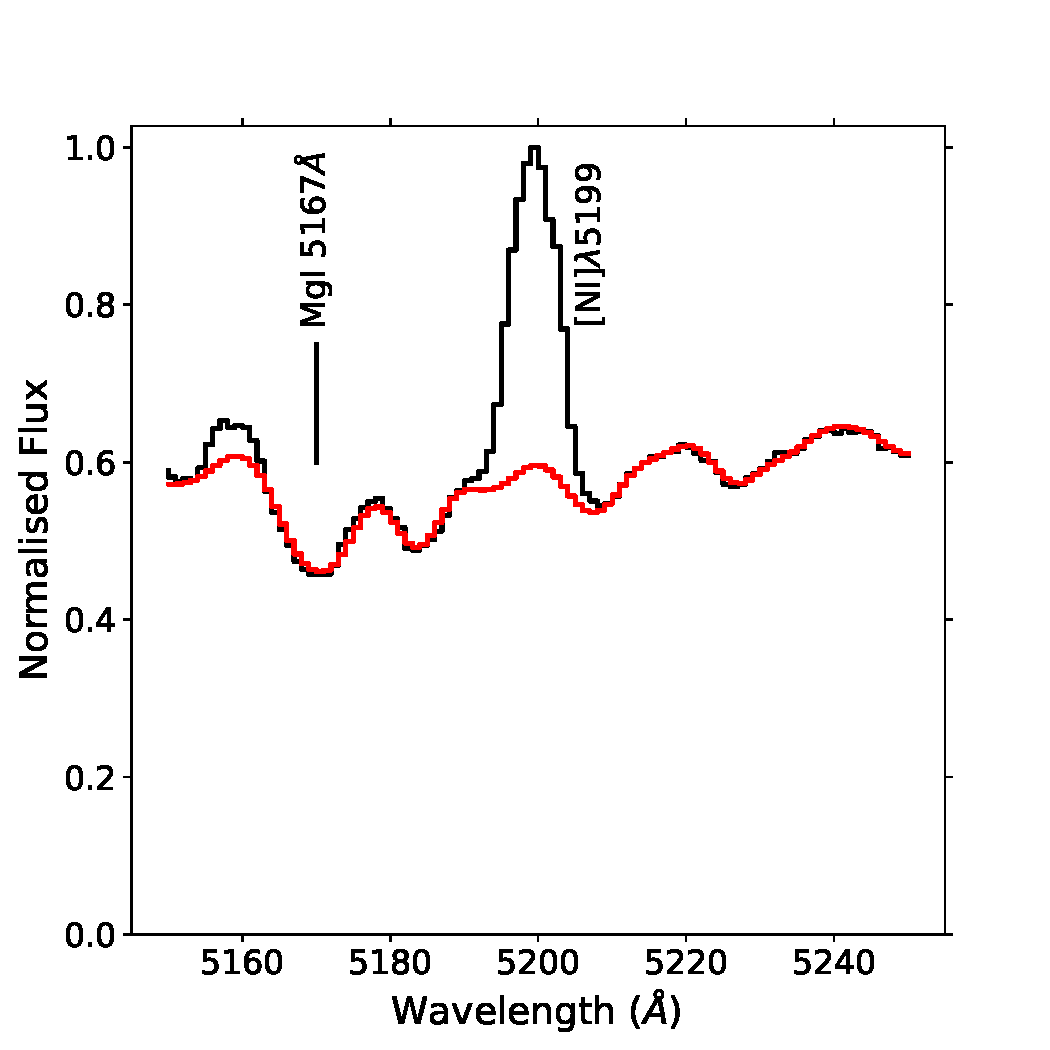
\includegraphics[width=\linewidth]{figures/xshooter_ic5063/starlight_mgi_ni.pdf}
        \caption{The spectral region of the MgI 5167\;{\AA} absorption feature and the [NI]$\lambda$5199 emission line.}
        \label{fig: xshooter_ic5063: starlight_mgi_ni}
    \end{subfigure}
    \hfill
    \begin{subfigure}[t]{0.47\textwidth}
        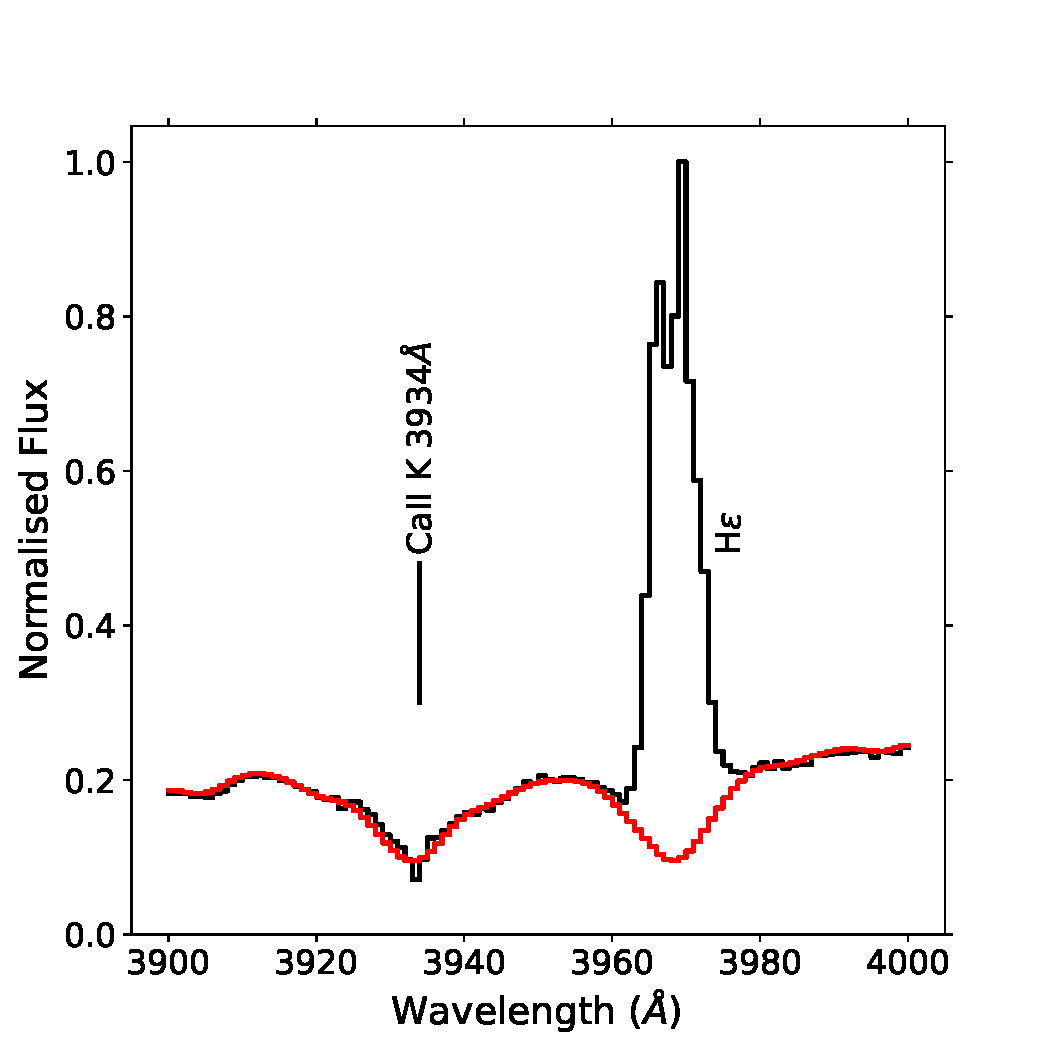
\includegraphics[width=\linewidth]{figures/xshooter_ic5063/starlight_caii_hk_hep.pdf}
        \caption{The spectral region of the CaII K absorption feature at 3934\;{\AA}, and the H$\mathrm{\varepsilon}$ recombination line.}
        \label{fig: xshooter_ic5063: starlight_caii_hk_heta}
    \end{subfigure}
    \vspace{2cm}
    \begin{subfigure}[t]{0.47\textwidth}
        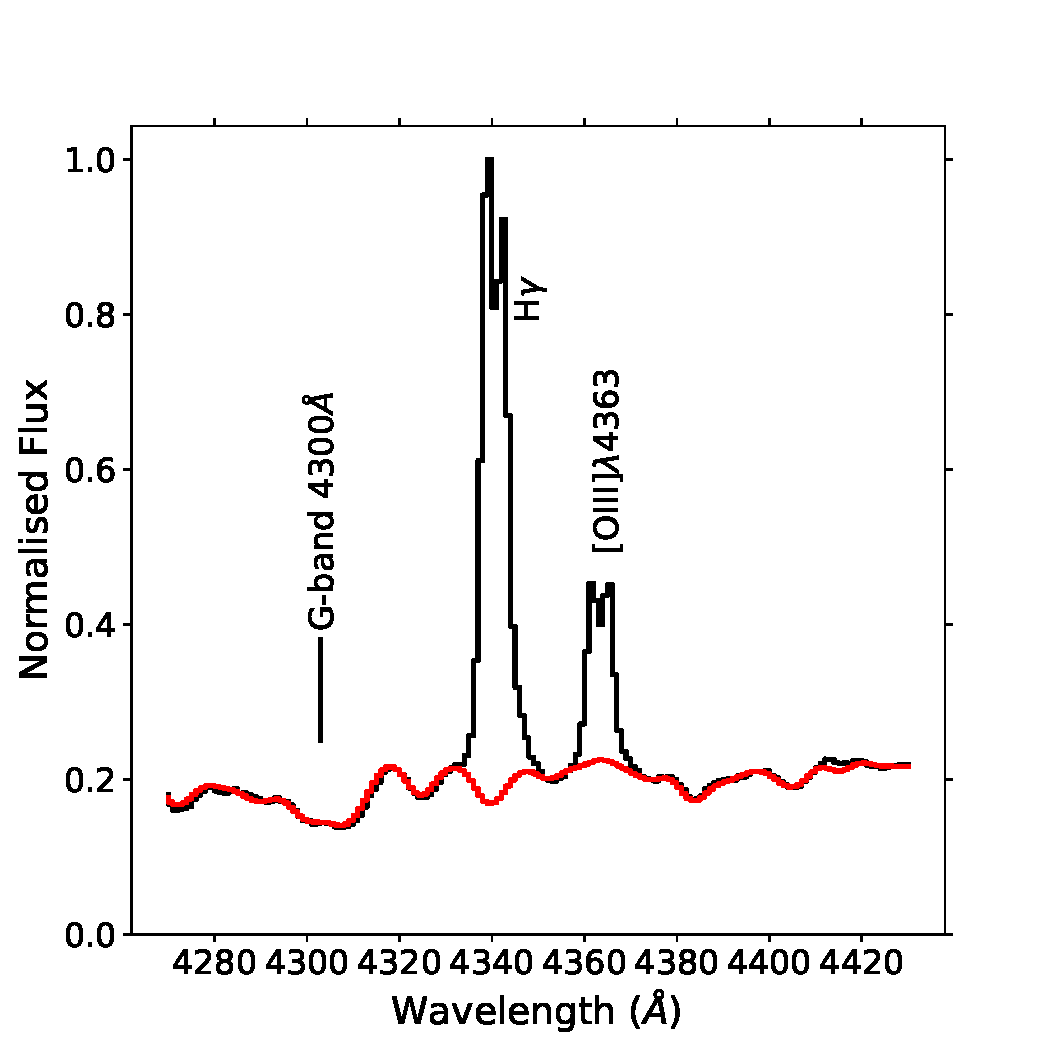
\includegraphics[width=\linewidth]{figures/xshooter_ic5063/starlight_hgamma_oiii4363.pdf}
        \caption{The spectral region of the H$\mathrm{\gamma}$ and [OIII]$\lambda$4363 emission lines; the fit to the G-band stellar absorption feature at $\sim$4300\;{\AA} can also be seen.}
        \label{fig: xshooter_ic5063: starlight_hgamma_oiii}
    \end{subfigure}
    \hfill
    \begin{subfigure}[t]{0.47\textwidth}
        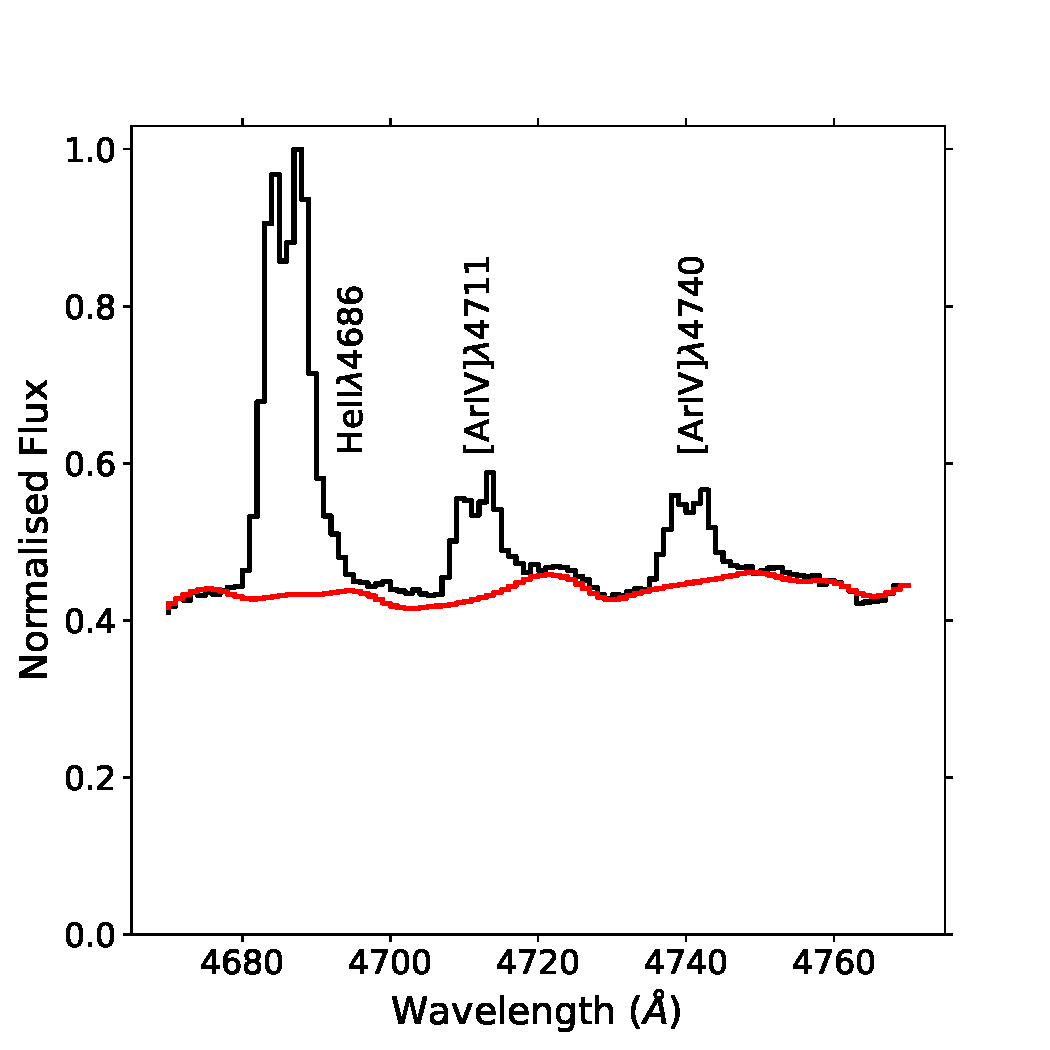
\includegraphics[width=\linewidth]{figures/xshooter_ic5063/starlight_ariv.pdf}
        \caption{The spectral region of the HeII$\lambda$4686 and [ArIV]$\lambda\lambda$4711,4740 emission lines.}
        \label{fig: xshooter_ic5063: starlight_heii_ariv}
    \end{subfigure}
    \vspace{-1.5cm}
    \caption[\textsc{STARLIGHT} stellar-synthesis fits to various key spectral features in Xshooter spectra of IC\;5063.]{\textsc{STARLIGHT} fits (red solid line) to various features in the spectrum extracted from Aperture 3 of the Xshooter UVB+VIS data (solid black line); the emission and absorption lines shown in each plot are labelled. Complex stellar continuum structure, which may significantly affect the derived line fluxes, can be seen underneath emission lines in several cases, and contributes significantly to the profiles of the [ArIV] lines. Therefore, proper modelling and subtraction was necessary to ensure accurate measurements of line fluxes.}
\end{figure*}

\subsection{Emission-line fitting}
\label{section: xshooter_ic_5063: observations_and_data_reduction: emission_line_fitting}

After stellar-continuum subtraction, the profiles of key emission lines in each aperture were fit with Gaussian profiles and a low-order-polynomial (to account for non-stellar continua in the UVB+VIS arms, and overall continuum structure in the NIR arm) using \textsc{Python} scripts written with the \textsc{NumPy} \citep{Harris2020}, \textsc{Pandas} \citep{reback2020pandas}, \textsc{AstroPy}, and \textsc{specutils} packages. In all cases, several Gaussian components were required to properly fit the emission-line profiles, however, to prevent overfitting, it was important to only use as few Gaussians as possible while still producing an adequate fit to the line profiles. Therefore, further Gaussian components were only added if they significantly reduced the mean-square residuals and $\chi^2$ of the fit. Furthermore, a sum-of-squares f-test \citep{Montgomery2012} was used to ensure that the relative decrease in residuals with each added Gaussian component was statistically significant (at the $\alpha=0.01$ significance level). This took into account the degrees of freedom of the total model when adding additional Gaussian components, preventing overfitting.

Emission-line-profile models for the combined UVB+VIS data were produced by first fitting the [OIII]$\lambda\lambda$4959,5007 doublet. Gaussian components were simultaneously fitted to both lines in the doublet, with each pair of Gaussian components having the same FWHM, and a wavelength separation (49.9\;{\AA}) and intensity ratio ($1:2.99$) defined by atomic physics \citep{Osterbrock2006}. The resulting multiple-Gaussian-component fits to the [OIII]$\lambda\lambda$4959,5007 doublet are hereafter referred to as the `[OIII] models'; these are shown for each aperture in Figure\;\ref{fig: xshooter_ic5063: o3_models}. For each aperture, narrow (FWHM$_\mathrm{w}$\;\textless\;200\;km\;s$^{-1}$: see Section\;\ref{section: xshooter_ic5063: properties_of_outflowing_gas: uvb_vis_analysis_and_results: kinematics}) and broad (FWHM$_\mathrm{w}$\;\textgreater\;500\;km\;s$^{-1}$) components of the [OIII] line profiles were identified. The former have kinematics consistent with gravitational (rotational) motions in the host galaxy (as deduced from large-scale HI\;21\;cm and CO kinematics: \citealt{Morganti1998, Morganti2015}), and the latter are consistent with outflowing gas. The broad components have complex, often multi-peaked profiles that required fitting with a combination of Gaussian components of different widths. Note that the \textit{individual} Gaussian components used to fit the broad components are not interpreted as physically-distinct kinematic components --- rather, they are required to account for the \textit{total} flux in the broad part of the line profiles.

Whereas in most apertures the [OIII] profiles can be well-described by one total broad and one total narrow component (each modelled with more than one Gaussian component), Aperture\;3 is an exception to this because there are two clearly separated `narrow' components and a single broad component in the [OIII]$\lambda\lambda$4959,5007 line profiles. In this case, the two narrow components are considered separately, and are labelled `Narrow 1' (red-most) and `Narrow 2' (blue-most). In apertures 4 and 5, the majority of the components are broad and heavily blended, and therefore only the total line fluxes (narrow + broad) are considered.

The [OIII] models were used to constrain the fits to the other UVB+VIS emission lines used in this analysis, namely H$\mathrm{\beta}$, H$\mathrm{\gamma}$, [OIII]$\lambda$4363, [OII]$\lambda$3726,3729, [OII]$\lambda\lambda$7319,7331, [SII]$\lambda\lambda$4068,4076, [SII]$\lambda\lambda$6717,6731, [ArIV]$\lambda\lambda$4711,4740 and HeII$\lambda$4686 --- the fits to these lines for Aperture 3 are shown in Figure\;\ref{fig: xshooter_ic5063: o3_models_all_lines}. I note that fits for H$\mathrm{\alpha}$ and the [NII]$\lambda\lambda$6548,6583 doublet were not produced for apertures with complex, broad emission-line profiles, as the lines were significantly blended and thus it was not possible to precisely measure their fluxes due to degeneracy issues. For all fits to the other lines, the intensity of each Gaussian component was allowed to vary, while the wavelength separations\footnote{When fitting the [OIII] models to other lines, the centroid wavelength of the brightest narrow component was allowed to vary by $\pm$1{\;\AA} in order to provide a better fit within the limit of the $\Delta\lambda$ = 1{\;\AA} resampling.} and widths of the Gaussian components were fixed. For some of the weaker emission lines with much lower fluxes than the [OIII]$\lambda\lambda$4959,5007 doublet, the fainter Gaussian components were sometimes excluded from the fits since the line-profile features they accounted for were extremely faint relative to the continuum.

For the emission lines that were fitted, including the transauroral [SII]$\lambda\lambda$4068,4076 and [OII]$\lambda\lambda$7319,7331 doublets, it was found that the [OIII] models describe their profiles well in all cases. In contrast, it was found that the [OIII] models do not describe emission lines in the NIR arm well, such as [FeII]$\lambda$12570, [FeII]$\lambda$16400, H$_2 \lambda$21218, Pa$\beta$, Br$\gamma$ and HeI$\lambda$10830. This is likely a result of the lack of stellar continua subtraction for the NIR data, which is due to the limited wavelength range of the \textsc{STARLIGHT} fits (3220--8000\;\AA), the lower cosmetic quality of the NIR spectra, and the difficulty in exactly matching the NIR apertures to the UVB+VIS apertures spatially. Therefore, each line in the NIR arm was fitted independently. \\

\begin{figure*}
	\includegraphics[width=\linewidth, trim={0cm 0cm 1cm 0cm},clip]{figures/xshooter_ic5063/oiii_models.png}
	\caption[{[}OIII{]} line profile models for the apertures extracted along the radio axis of Xshooter spectra of IC\;5063.]{[OIII]$\lambda\lambda$4959,5007 rest-frame line profiles and models for the apertures covering the inner regions of IC\;5063. The observed line profiles are shown in black, the overall fits to the profiles are shown as red solid lines, the Gaussian components comprising the total narrow component are shown as blue dashed lines, and the Gaussian components comprising the total broad component are shown as dotted green lines. Fitting residuals are shown as black dots below each line profile. In the cases of apertures 4 and 5, each Gaussian component is shown as a purple dash-dotted line, as there is no distinction made between broad and narrow. The wavelengths corresponding to the percentile ($v_\mathrm{p}$; $v_\mathrm{05}$ and $v_\mathrm{95}$) and the flux-weighted velocities ($v_\mathrm{w}$) for Aperture 5 are shown as dashed grey lines. For Aperture 6, dashed grey lines mark the wavelengths of the percentile velocity of the broad component ($v_\mathrm{p,b}$) and flux-weighted velocity of the narrow component ($v_\mathrm{w,n}$) --- these are used to calculate the outflow velocity ($v_\mathrm{out}$ = $v_\mathrm{p,b}$ - $v_\mathrm{w,n}$). Aperture 3 presents two clearly split narrow components, which are labelled `Narrow 1' (red-most) and `Narrow 2' (blue-most).}
	\label{fig: xshooter_ic5063: o3_models}
\end{figure*}

\begin{figure*}
	\includegraphics[width=\linewidth]{figures/xshooter_ic5063/oiii_fits_other_lines.png}
	\caption[{[}OIII{]}-model fits to key emission lines used in the analysis of Xshooter observations of IC\;5063.]{Fits to key diagnostic emission lines in Aperture 3 of the UVB+VIS spectra using the [OIII] model for Aperture 3 (shown in Figure\;\ref{fig: xshooter_ic5063: o3_models}). Where lines from multiple atoms are present, they are labelled by both atom and species. The diagnostic lines shown here are used in this chapter to derive key outflow properties.}
	\label{fig: xshooter_ic5063: o3_models_all_lines}
\end{figure*}

\newpage

\section{Properties of the outflowing gas}
\label{section: xshooter_ic5063: properties_of_outflowing_gas}

\subsection{Analysis of the UVB+VIS apertures}
\label{section: xshooter_ic5063: properties_of_outflowing_gas: uvb_vis_analysis_and_results}

\subsubsection{Velocity shifts and widths}
\label{section: xshooter_ic5063: properties_of_outflowing_gas: uvb_vis_analysis_and_results: kinematics}

The Doppler shifts and widths of broad and narrow components of the [OIII] models, relative to the lab wavelength\footnote{Note that the Xshooter spectra were de-redshifted, as described in Section\;\ref{section: xshooter_ic_5063: observations_and_data_reduction: data_reduction}.} of [OIII]$\lambda$5007, were used to determine outflowing and quiescent (non-outflowing) gas kinematics. First, the instrumental broadening (as measured from the Galactic NaID lines) was subtracted from the width of each component in quadrature in order to produce the intrinsic line widths.

When deriving outflow kinematics, projection effects must be carefully considered (see Section\;\ref{section: introduction: outflows: kinematics_and_geometry: kinematics}). Therefore, two methods for estimating outflow velocity were used, giving `minimal' and `maximal' velocities, following the methodology presented by \citet{Rose2018}. The first approach was to calculate flux-weighted mean velocity shifts and widths --- this was done for the total broad and narrow components by weighting the centroid velocities and FWHM of each constituent Gaussian component by its total flux:

\begin{equation}
v_\mathrm{w} = \frac{\Sigma_i(F_i \times v_i)}{\Sigma_i{F_i}}\text{, and}
\label{eq: xshooter_ic5063: flux_velocity}
\end{equation}

\begin{equation}
\mathrm{FWHM_w} = \frac{\Sigma_i(F_i{\times}\mathrm{FWHM_i})}{\Sigma_i{F_i}},
\label{eq: xshooter_ic5063: flux_width}
\end{equation}
\noindent
where $F_\mathrm{i}$, FWHM$_\mathrm{i}$ and $v_\mathrm{i}$ are the fluxes, FWHMs and velocity shifts of the constituent Gaussian components, respectively. Velocity shifts were calculated using the wavelength shifts of a given centroid to the lab wavelength of [OIII]$\lambda$5007; for the broad components, this is likely to underestimate true outflow velocities.

Percentile velocities were also derived by using the far wings of the broad-component profiles, as described in Section\;\ref{section: introduction: outflows: kinematics_and_geometry: kinematics}. Here, it is assumed that all line broadening is due to different projections of velocity vectors along the line of sight, rather than intrinsic velocity dispersion in the gas in each volume element. In this case, the extended velocity wings represent gas moving directly along the line of sight, and potentially give a better estimate of the true outflow velocity. Therefore, velocity widths are not reported in this case. Percentile velocity shifts were determined for the broad components using the wavelength which contains either 5 or 95 per cent of the total flux of the line profile relative to the lab wavelength of [OIII]$\lambda$5007 (whichever velocity was greater, to ensure that outflow kinematics were not underestimated). Velocities derived in this way are labelled $v_\mathrm{p}$. As an example, in Figure\;\ref{fig: xshooter_ic5063: o3_models} both the percentile ($v_\mathrm{p}$) and flux-weighted ($v_\mathrm{w}$) velocity for the [OIII] profile of Aperture 5 are shown.

\begin{table*}
	\renewcommand{\arraystretch}{1}
	\begin{tabular}{lcccccc}
	\multirow{2}{*}{Component} & Distance   & Distance  & $v_\mathrm{p}$  & $v_\mathrm{w}$  & FWHM$_\mathrm{w}$     & $v_\mathrm{out}$  \\ 
        & (arcsec) & (kpc) & (km\;s$^{-1}$) & (km\;s$^{-1}$) & (km\;s$^{-1}$) & (km\;s$^{-1}$) \\
        \\
    \hline \\
	AP1 Narrow       & $-$4.72             & $-$1.09          & ---    & 218$\pm$5    & 120$\pm$3  &                  \\
		&	&	&	&	&	&	\\
	AP2 Narrow       & $-$3.44             & $-$0.79          & ---    & 197$\pm$3    & 110$\pm$2  &                  \\
		&	&	&	&	&	&	\\
	AP3 Narrow 1     & $-$1.84             & $-$0.43          & ---    & 166$\pm$3    & 158$\pm$4  &                  \\
	AP3 Narrow 2     & $-$1.84             & $-$0.43          & $-$202$\pm$2   & $-$68$\pm$1    & 187$\pm$3  & $-$233$\pm$4$^a$   \\
	AP3 Broad        & $-$1.84            & $-$0.43          & 507$\pm$23   & 121$\pm$8    & 549$\pm$36 & 341$\pm$23   \\ 
		&	&	&	&	&	&	\\
	AP4 Total        & 0                 & 0              & 264$\pm$41   & $-$7$\pm$2     & 296$\pm$16 &                  \\
		&	&	&	&	&	&	\\
	AP5 Total        & 1.36              & 0.31           & $-$699$\pm$173 & $-$102$\pm$8   & 670$\pm$27 & $-$699$\pm$173$^b$ \\
		&	&	&	&	&	&	\\
	AP6 Narrow       & 2.08              & 0.48           & ---   & $-$193$\pm$4   & 102$\pm$4  &                  \\
	AP6 Broad        & 2.08              & 0.48           & $-$714$\pm$156 & $-$198$\pm$15  & 614$\pm$58 & $-$521$\pm$156 \\
		&	&	&	&	&	&	\\
	AP7 Narrow       & 3.04              & 0.70           & ---  & $-$166$\pm$4   & 163$\pm$4  &                  \\
	AP7 Broad        & 3.04              & 0.70           & $-$624$\pm$85  & $-$166$\pm$13  & 627$\pm$57 & $-$457$\pm$85   \\ 
		&	&	&	&	&	&	\\
	AP8 Narrow       & 4.48              & 1.03           & ---  & $-$197$\pm$17 & 157$\pm$18 &                  \\
		&	&	&	&	&	&	\\
	\end{tabular} \\
	$^a$ calculated using the flux-weighted velocities ($v_\mathrm{w}$) for AP3 Narrow 1 (quiescent gas) and AP3 Narrow 2 (in/out-flowing gas). \\
	$^b$ the same as the percentile velocity ($v_\mathrm{p}$) since there is no corresponding narrow component.\\
	\caption[Warm-ionised gas kinematics along the radio structure of IC\;5063.]{The kinematics for the broad and narrow components in each aperture, including the percentile velocities ($v_\mathrm{p}$; the velocity that contains 5 or 95\;per\;cent of the flux of the emission-line profile), flux-weighted velocities ($v_\mathrm{w}$; determining used flux-weighted velocity averages), and corresponding flux-weighted velocity widths (FWHM$_\mathrm{w}$). The outflow velocity ($v_\mathrm{out}$) is taken to be the difference between the percentile velocity of the outflowing broad components and the flux-weighted velocity of the quiescent narrow components at each position. The distances from the centre of Aperture 4 (the nucleus) to the centre of the aperture for each component are also given in both arcseconds and kpc. For Aperture 3, `Narrow 1' and `Narrow 2' denote the two narrow components of the split line profile (see Figure\;\ref{fig: xshooter_ic5063: o3_models}), with `Narrow 2' being the blue-most narrow component}
	\label{tab: xshooter_ic5063: kinematics}
\end{table*}

\begin{figure*}
    \centering
	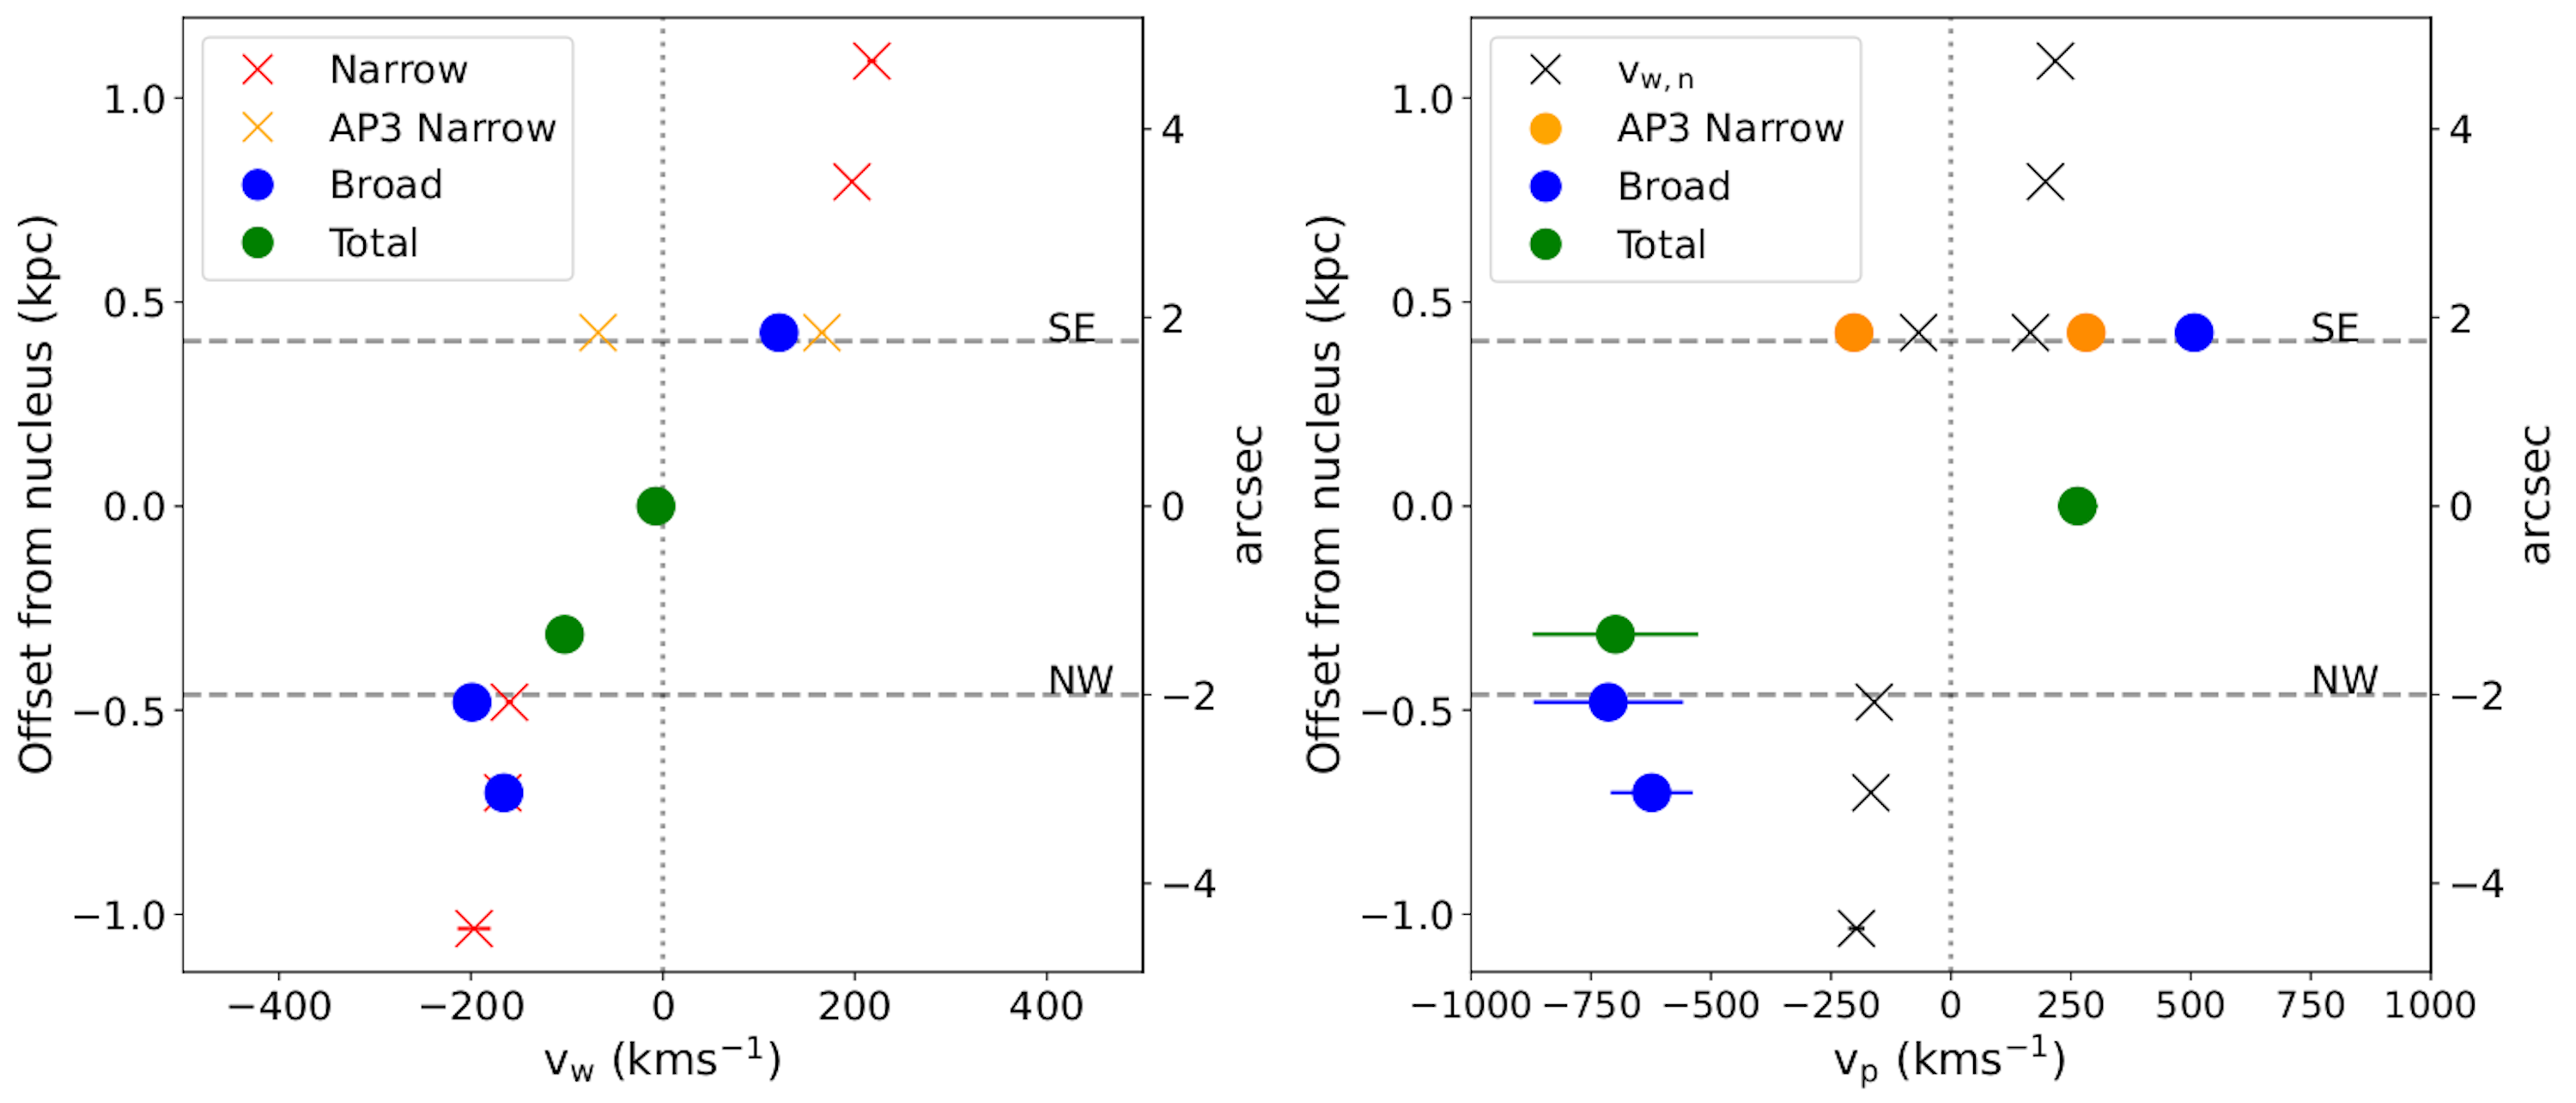
\includegraphics[width=\linewidth]{figures/xshooter_ic5063/vmin_vmax.png}
	\caption[Velocity shifts of the warm-ionised gas along the radio structure of IC\;5063.]{Velocity shifts for narrow (red crosses), broad (blue circles), and total (green circles) kinematic components in each aperture, shown spatially across the radio structure of IC\;5063. The split narrow components in Aperture 3 are shown in orange. The spatial position of each component corresponds to the centre of the aperture in which it was measured. \textbf{Left}: flux-weighted velocities of the narrow and broad components --- the narrow components are taken to represent the galaxy's quiescent rotating gas disk. \textbf{Right}: percentile velocity shifts ($v_\mathrm{p}$) for the broad components, taken to represent outflowing gas, compared with the flux-weighted velocities of the narrow components ($v_\mathrm{w,n}$, shown for reference as black crosses). The dashed grey lines mark the centroids of the NW and SE radio lobes, measured from 24.8\;GHz continuum imaging presented by \citet{Morganti2007}. A velocity shift of zero relative to the galaxy's rest frame is marked with a grey dotted line.}
	\label{fig: xshooter_ic5063: velocities}
\end{figure*}

\begin{figure}
    \centering
	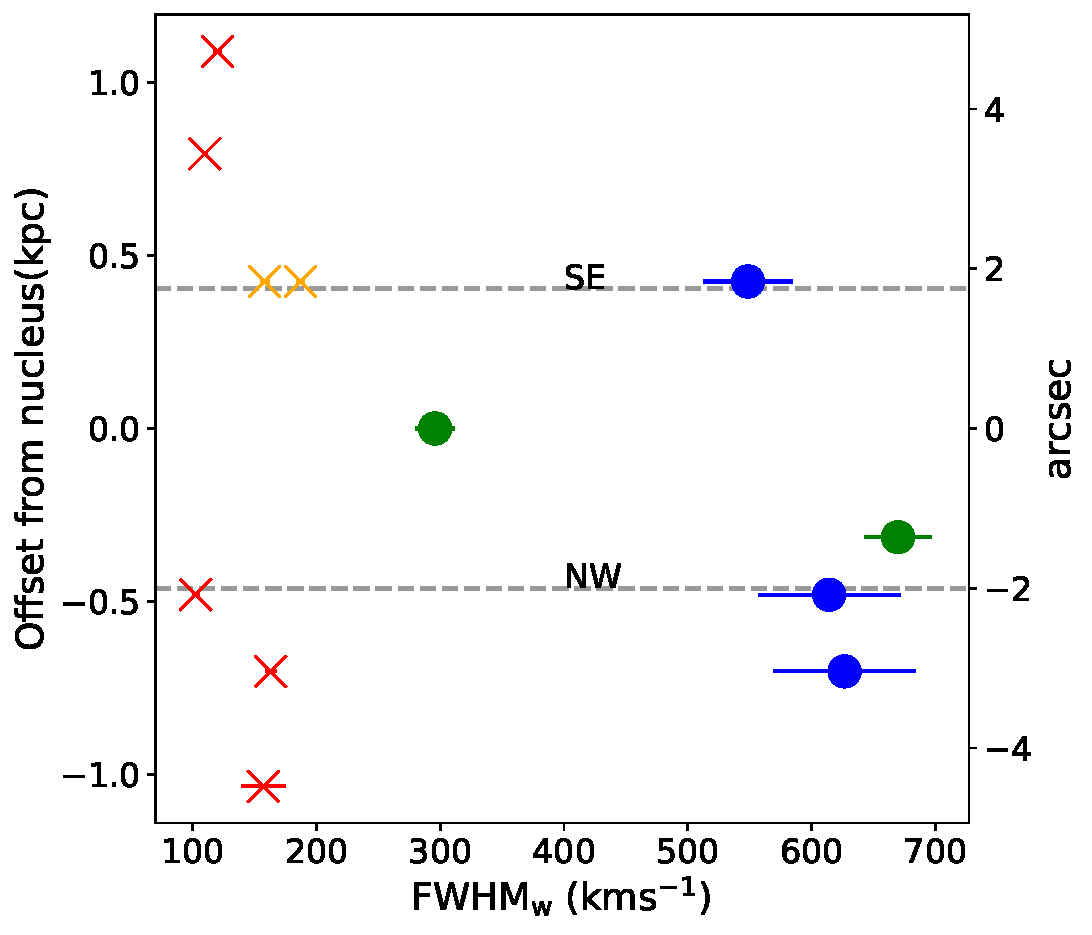
\includegraphics[width=0.55\linewidth]{figures/xshooter_ic5063/vmin_widths.pdf}
	\caption[Velocity widths of the warm-ionised gas along the radio structure of IC\;5063.]{Flux-weighted velocity widths (FWHM$_\mathrm{w}$) as determined in the minimal velocity case, in which the measured velocity widths are assumed to be entirely due to local velocity dispersion within the outflow. The colour and marker scheme and dashed lines are the same as in Figure\;\ref{fig: xshooter_ic5063: velocities}.}
	\label{fig: xshooter_ic5063: fwhm}
\end{figure}

\newpage
Figure\;\ref{fig: xshooter_ic5063: velocities} shows a position-velocity (PV) diagram of the percentile ($v_\mathrm{p}$) and flux-weighted ($v_\mathrm{w}$) velocity shifts, as measured in each aperture, and Figure\;\ref{fig: xshooter_ic5063: fwhm} shows the flux-weighted velocity widths. In the flux-weighted case ($v_\mathrm{w}$; right panel of Figure\;\ref{fig: xshooter_ic5063: velocities}), the velocity shifts of the narrow components (with the exception of the blue-most narrow component in Aperture 3) appear to follow a rotation curve of amplitude $\pm$218\;km\;s$^{-1}$, corresponding to the rotational motion of the galaxy's disk (as seen in HI\;21\;cm and CO observations: \citealt{Morganti1998, Morganti2015, Oosterloo2017}). Deviations from this rotation curve can be seen in the percentile velocity shifts of the broad components and the total line profile in Aperture 5 (which is dominated by broad components), indicating that the broad components represent outflowing gas. Interestingly, this deviation is not seen in the flux-weighted case, indicating that the outflows are kinematically symmetric relative to the disk rotation. 

One of the narrow components observed in the line profile of Aperture 3 (`AP3 Narrow 2') shows significant deviation ($v\sim350$\;km\;s$^{-1}$) from the rotation curve, indicating that it is a distinct kinematic component which may represent outflowing or inflowing gas. 

From these kinematics, the broad components in apertures 3, 6 and 7, along with the `AP3 Narrow 2' component and the total line profile of Aperture 5, are taken to represent outflowing gas. Note that the broad components in apertures 1, 2 and 8 are most likely due to spill-over from the broad profiles in the central apertures due to the beam-smearing effect of atmospheric seeing --- not locally outflowing gas --- and as such are not considered to represent outflows at these locations. Since the kinematics of the narrow components are consistent with quiescent gas in a rotating disk, the outflow velocity in each aperture was thus taken to be the difference between the percentile velocity ($v_\mathrm{p}$) of the broad component (outflow) and the flux-weighted velocity ($v_\mathrm{w}$) of the narrow component (quiescent) --- an example of this for Aperture 6 is shown in Figure\;\ref{fig: xshooter_ic5063: o3_models}. For Aperture 5, where the majority of the components are broad and the narrow components (representing emission from the rotating disk) are heavily blended, the outflow velocity is taken to be the percentile velocity. The derived flux-weighted, percentile, and outflow velocities (in addition to the velocity widths) are given in Table\;\ref{tab: xshooter_ic5063: kinematics}.

\subsubsection{Spatial distributions and kinematics of optical diagnostic lines}
\label{section: xshooter_ic5063: properties_of_outflowing_gas: uvb_vis_analysis_and_results: spatial_distributions}

\begin{table}
    \vspace*{1cm}
	\centering
	\renewcommand{\arraystretch}{1.5}
	\begin{tabular}{ccc}
	Emission Line           &  Centroid (pixels) & Centroid (arcsec) \\ \hline
	[OIII]$\lambda$5007 & 12.3$\pm$0.1                                                                                                       & 1.97$\pm$0.02                                                                                                             \\
	H$\beta$                & 12.5$\pm$0.1                                                                                                       & 2.00$\pm$0.02                                                                                                             \\
	{[}OII{]}$\lambda$7319  & 11.9$\pm$0.1                                                                                                       & 1.90$\pm$0.02                                                                                                             \\
	{[}SII{]}$\lambda$4069  & 12.0$\pm$0.1                                                                                                       & 1.92$\pm$0.02                                                                                                            
	\end{tabular} \\
	\caption[The spatial positions of the peak flux of the blue wings of the transauroral {[}OII{]} and {[}SII{]} lines, in addition to {[}OIII{]}$\lambda5007$ and H$\beta$ lines]{Centroids of Gaussian fits to spatial slices between \mbox{$-$600\;\textless\;$v$\;\textless\;$-$400\;km\;s$^{-1}$} of the transauroral [OII] and [SII] emission lines, along with H$\mathrm{\beta}$ and [OIII]$\lambda$5007 (shown in Figure\;\ref{fig: xshooter_ic5063: spatial_optical}), relative to the spatial position of the continuum centre.}
	\label{tab: xshooter_ic5063: spatial_vis}
\end{table}

\begin{figure}[!ht]
    \vspace*{1cm}
	\centering
	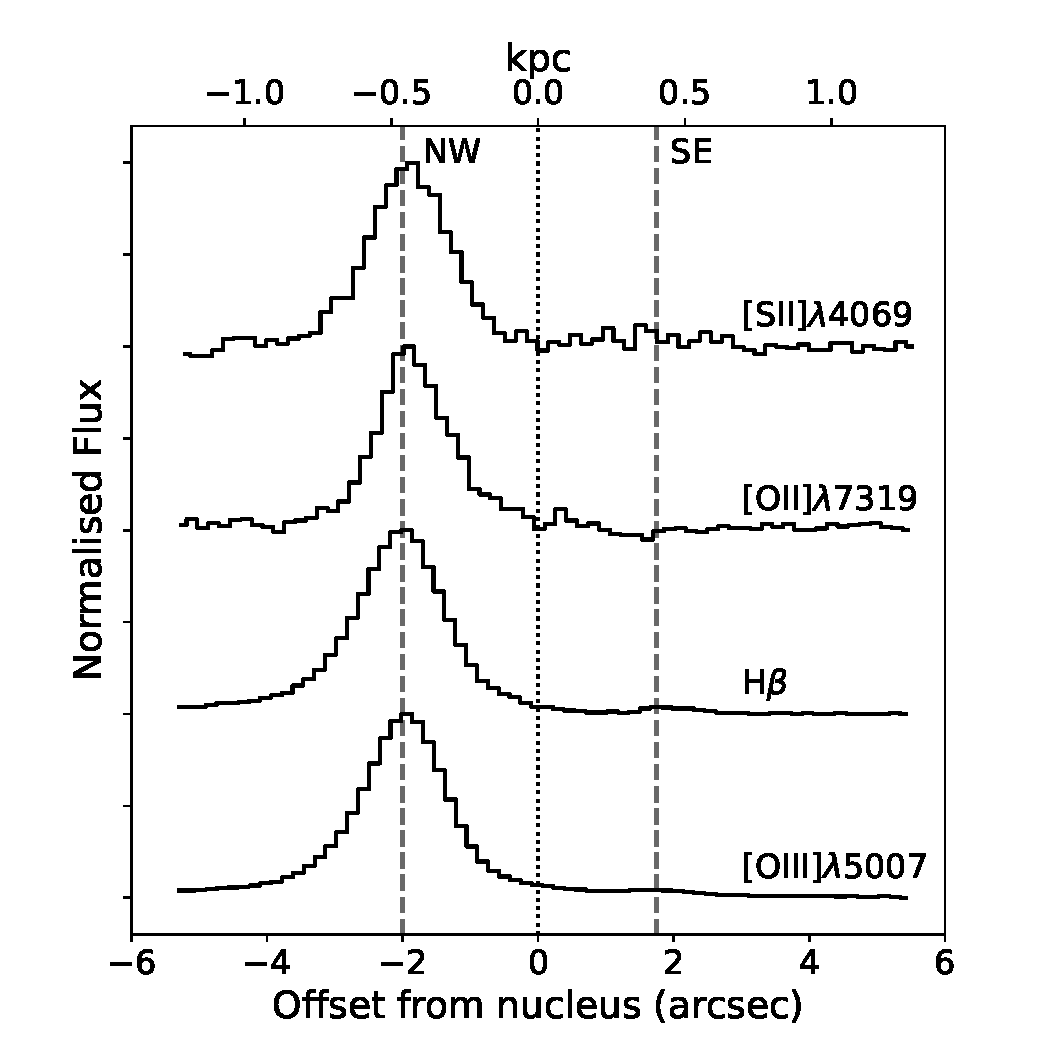
\includegraphics[width=0.7\linewidth]{figures/xshooter_ic5063/spatial_optical_labeled.pdf}
	\caption[Spatial distributions of the blue wings of the transauroral {[}OII{]} and {[}SII{]} lines, in addition to {[}OIII{]}$\lambda5007$ and H$\beta$ lines along the radio axis of IC\;5063.]{Spatial distributions of the blue wings (\mbox{$-$600\;\textless\;$v$\;\textless\;$-$400\;km\;s$^{-1}$}) of the transauroral [SII] and [OII] lines, H$\mathrm{\beta}$, and [OIII]$\lambda$5007 emission lines. The spatial flux distribution of the transauroral lines can be seen to closely follow those of [OIII] and H$\mathrm{\beta}$. The dotted line shows the position of the nucleus, and the dashed lines show the positions of the centroids of the NW and SE radio lobes, as measured from 24.8\;GHz imaging presented by \citet{Morganti2007}.}
	\label{fig: xshooter_ic5063: spatial_optical}
    \vspace*{1cm}
\end{figure}

Previous studies that make use of the transauroral lines to derive electron densities have been spatially unresolved (e.g. \citealt{Holt2011, Rose2018, Santoro2018, Spence2018, Santoro2020, Davies2020}), and it has not yet been verified that the transauroral lines are emitted by the same clouds as other key diagnostic lines such as [OIII]$\lambda$5007 and H$\mathrm{\beta}$ (see discussion in Section\;\ref{section: introduction: outflows: energetics: electron_densities}). However, from the Xshooter spectra presented here, it is found that the [OIII] models provide good fits to the lines used in this analysis, including the transauroral [SII] and [OII] doublets (Figure\;\ref{fig: xshooter_ic5063: o3_models_all_lines}). This demonstrates that these lines have similar profiles and thus similar kinematics, potentially indicating that they are emitted by the same cloud systems. To verify this, spatial slices of the blue wings of several key emission lines in the velocity range \mbox{$-$600\;\textless\;$v$ \;\textless\;$-$400\;km\;s$^{-1}$} were extracted from the two-dimensional spectra, avoiding any narrow components of the line profiles. Slices of continuum emission were also extracted, free from any emission lines, both blue-ward and red-ward of each emission line with slice widths of 20\;\AA. The two continuum slices were added and scaled to account for the different number of pixel columns extracted from the blue wing of each line --- the average continuum slice was then subtracted from the blue wing. The spatial position of the nucleus at the wavelength of each line was determined using Gaussian fits to the continuum spatial slices, and the peak positions of the extended emission line structures were then measured relative to this estimated nucleus position using Gaussian fits. Spatial flux distributions produced in this way are presented in Figure\;\ref{fig: xshooter_ic5063: spatial_optical}, and the peak centroid positions of the extended line emission from the Gaussian fits are given in Table\;\ref{tab: xshooter_ic5063: spatial_vis}.

From this analysis, it can be seen that the spatial flux profiles for the transauroral [OII] and [SII] lines are similar to those of the [OIII]$\lambda$5007 and H$\mathrm{\beta}$ lines. Furthermore, the values of the fitted Gaussian centroids for the peak of each line are consistent within 0.6\;pixels, a remarkable result given the known uncertainties from the Gaussian fitting process and the unknown systematic uncertainties from the continuum subtraction process, which will affect the lower-flux transauroral lines more than the brighter [OIII] and H$\mathrm{\beta}$ lines. In addition to the [OIII] models fitting the transauroral-line profiles well, this is taken as evidence that the transauroral lines are emitted in the same spatial locations as other key diagnostic lines. However, the possibility of the lines being emitted by different clouds within the same spatial apertures cannot be entirely ruled out.

\subsubsection{Transauroral-line diagnostics}
\label{section: xshooter_ic5063: properties_of_outflowing_gas: uvb_vis_analysis_and_results: transauroral_lines}

The high spectral resolution and wide wavelength coverage of the Xshooter observations allow the use of a technique first presented by \citet{Holt2011}, which employs the traditional and transauroral [OII] and [SII] lines to simultaneously derive values for electron density and reddening. This is done by comparing the following emission-line-flux ratios to those expected from photoionisation modelling:
\begin{align*}
TR([OII]) = F(3726 + 3729) / F(7319 + 7331), \\
TR([SII]) = F(4068 + 4076) / F(6717 + 6731).
\end{align*} 

A major advantage of this technique is that the \textit{total} line fluxes of the doublets are used for the ratios, instead of the flux ratios of lines \textit{within} the doublets (as is the case for traditional techniques of electron-density estimation) which are sensitive to blending effects at larger line widths. The [OIII] models were used as bases for the fits to the lines involved in the TR([OII]) and TR([SII]) ratios. In order to avoid additional issues due to degeneracy and blending owing to the complex kinematics, further constraints to the fits for a given kinematic component were applied in several ways. First, the widths of lines in a doublet were forced to be equal, and the wavelength separations between them were set to be those defined by atomic physics. Second, the intensity ratios of doublet lines were constrained in the following ways in order to ensure that the fits were not unphysical.
\begin{itemize}
	\item The ratios of the [OII]$\lambda\lambda$3726,3729, [SII]$\lambda\lambda$4049,4076, and [SII]$\lambda\lambda$6717,6731 doublets were forced to be within the range of their theoretical values \citep{Osterbrock2006, Rose2018}; if a measured intensity ratio was above or below this permitted range, it was forced to be the maximum or minimum allowed theoretical value, respectively.
	\item The intensity ratio of the [OII](7319/7330) ratio was set to be 1.24 because this ratio does not vary with density \citep{Rose2018}. Note that this doublet is actually two distinct doublets ([OII]$\lambda\lambda$7319,7320 and [OII]$\lambda\lambda$7330,7331); however, here they are modelled as single lines because their separation ($\sim$1\;{\AA}) is much lower than the widths of the narrowest kinematic components of the [OIII] models. Note that, while no broadening correction was made to account for the closely-spaced doublets, the [OIII] models still provided robust descriptions of the line profiles when considered as single lines (Figure \ref{fig: xshooter_ic5063: o3_models_all_lines}).
\end{itemize}

The \textsc{CLOUDY} photoionisation code (version C17.02: \citealt{Ferland2017}) was used to create single-slab, plane-parallel, radiation-bounded, and solar-composition models of photo-ionised gas with no dust depletion. The central photoionising continuum followed a power-law of shape $F_v \propto v^{-\alpha}$ between 10\;{\textmu}m and 50\;keV, with a spectral index of $\alpha=1.5$. This is close to the average optical-to-X-ray spectral index measured in radio-quiet AGN \citep{Zamorani1981, Miller2011}, and is consistent with photoionisation modelling of the emission-line ratios of the extended and nuclear NLRs in various samples of AGN (e.g. \citealt{Ferland1983}, \citealt{Robinson1987}). Ionisation parameters ($U$) were estimated for each aperture using estimated [OIII]/H$\mathrm{\beta}$ and [NII]/H$\mathrm{\alpha}$ line ratios with the relation presented by \citet{Baron2019b}: the resulting ionisation parameters were in the range \mbox{$-$2.90\;\textless\;log$U$\;\textless\;$-$2.45}. Therefore, log$U=-$2.75 was chosen for use in the \textsc{CLOUDY} models. The electron density of the modelled gas was varied by 0.1\;dex steps in the range \mbox{2.0\;\textless\;log$_{10}(n_\mathrm{e}$\;[cm$^{-3}$])\;\textless\;5.0}, and the CCM89 reddening law was used with $R_\mathrm{v}=3.1$ to redden these simulated TR ratios in order to create a grid with varying electron density and reddening. The resulting grid, along with the measured TR ratios in each aperture, is shown in Figure\;\ref{fig: xshooter_ic5063: tr_grid}, and the densities derived from this method are presented in Table\;\ref{tab: xshooter_ic5063: densities}. I note that these values were determined using a finer grid than is shown in Figure\;\ref{fig: xshooter_ic5063: tr_grid}.

\begin{figure}[!ht]
    \centering
	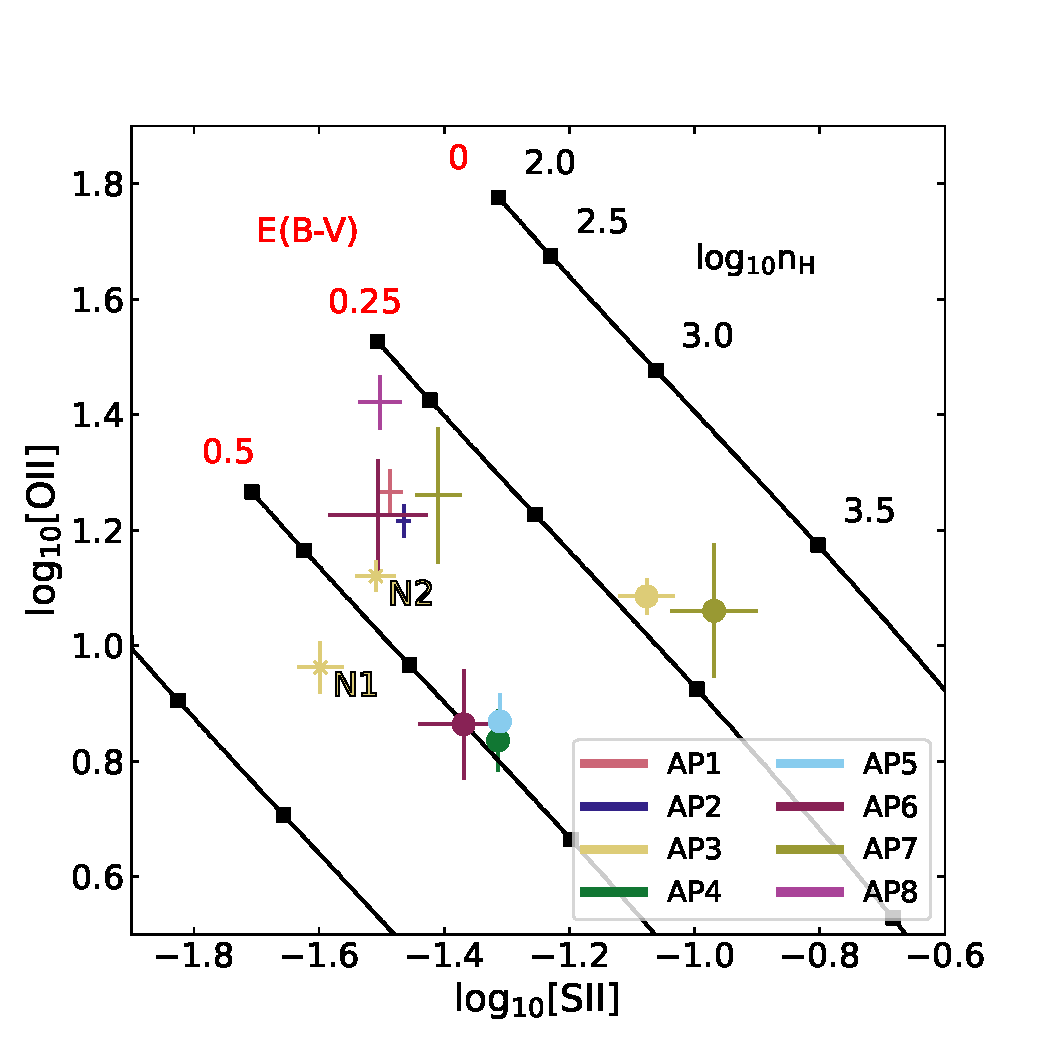
\includegraphics[width=0.75\linewidth]{figures/xshooter_ic5063/ddd_grid_zoomed.pdf}
	\caption[Transauroral {[}OII{]} and {[}SII{]} line ratio diagram for IC\;5063, showing both measured values and those predicted from photoionisation modelling.]{log$_{10}$ values of TR line ratios measured for the total narrow (crosses) and broad (circles) components in each aperture. Values for the total line profiles, as measured in apertures 4 and 5, are also shown as circles. The two narrow components in Aperture 3 are marked as `N1' and `N2'. Overlaid is a grid of simulated TR line ratios created using the \textsc{CLOUDY} photoionisation code (version C17.02, \citealt{Ferland2017}) for different values of electron density and reddened using the CCM89 reddening law, indicated by the joined series of black squares.}
	\label{fig: xshooter_ic5063: tr_grid}
\end{figure}

Using the transauroral line ratios, it is found that the broad components have significantly higher (\mbox{\textgreater\;3$\sigma$}) electron densities (\mbox{3.17\;\textless\;log$_{10}(n_\mathrm{e}$\;[cm$^{-3}$])\;\textless\;3.43}) than the narrow components (\mbox{2.12\;\textless\;log$_{10}(n_\mathrm{e}$\;[cm$^{-3}$])\;\textless\;2.59}) in all apertures where both are measured. In apertures 4 and 5 (where total line fluxes were used), the measured electron densities are consistent with those of the broad components in other apertures. Furthermore, in apertures where only a narrow component is measured (apertures 1, 2 and 8), densities similar to those of the narrow components in other apertures are found. The reddenings that are derived from the transauroral lines are moderately high (\mbox{0.17\;\textless\;E(B$-$V)$_{TR}$\;\textless\;0.51}), with no clear distinction between the values for narrow and broad components.

\begin{table*}
    \centering
	\def\arraystretch{1.5}
	\begin{tabular}{lcccc}
	\multirow{2}{*}{Component} & log$_{10}(n_\mathrm{e}$\;[cm$^{-3}$]) & log$_{10}(n_\mathrm{e}$\;[cm$^{-3}$]) & log$_{10}(n_\mathrm{e}$\;[cm$^{-3}$])  & log$_{10}(n_\mathrm{e}$\;[cm$^{-3}$])  \\ 
        & (TR) & ([OII]) & ([SII]) & ([ArIV]) \\
    \hline
	AP1 Narrow       & 2.53$^{+0.06}_{-0.07}$ & \textless\;2.13                                     & 1.97$^{+0.08}_{-0.10}$                    & 3.70$^{-0.27}_{+0.24}$      \\
		&	&	&	&	\\
	AP2 Narrow       & 2.65$^{+0.03}_{-0.04}$ & 2.02$^{+0.11}_{-0.14}$                    & \textless\;2.15                                     & \textless\;3.71                                        \\
	&	&	&	&	\\
	AP3 Narrow 1     & 2.59$^{+0.05}_{-0.05}$ & --- & --- & ---                   \\
	AP3 Narrow 2     & 2.55$^{+0.03}_{-0.03}$ & --- & --- & ---                  \\
	AP3 Broad        & 3.30$^{+0.05}_{-0.05}$ & --- & 2.84$^{+0.09}_{-0.09}$                    & ---    \\
	&	&	&	&	\\
	AP4 Total        & 3.25$^{+0.05}_{-0.05}$ & --- & ---  & 3.79$^{+0.18}_{-0.19}$   \\
&	&	&	&	\\
	AP5 Total        & 3.23$^{+0.04}_{-0.05}$ & --- & --- & \textless\;5.97 \\
&	&	&	&	\\
	AP6 Narrow       & 2.55$^{+0.16}_{-0.20}$ & --- & --- & ---   \\
	AP6 Broad        & 3.17$^{+0.09}_{-0.09}$ & --- & --- & ---    \\
&	&	&	&	\\
	AP7 Narrow       & 2.69$^{+0.15}_{-0.19}$ & --- & --- & ---    \\
	AP7 Broad        & 3.43$^{+0.09}_{-0.09}$ & --- & --- & ---    \\
&	&	&	&	\\
	AP8 Narrow       & 2.12$^{+0.14}_{-0.12}$ & 2.07$^{+0.11}_{-0.12}$  & 2.02$^{+0.14}_{-0.17}$ & \textless4.03  \\
	\end{tabular}
	\caption[Electron densities for the warm-ionised gas along the radio axis of IC\;5063, measured with the transauroral line technique, the traditional {[}SII{]} and {[}OII{]} line ratios, and the {[}ArIV{]}(4711/4740) ratio.]{Electron density values determined using the TR, traditional, and [ArIV] line ratios for the gas in IC\;5063. 3$\sigma$ upper limits are shown where the measured line ratio was not 3$\sigma$ from the lower or upper limit of the traditional line ratios. It was not possible to determine values for electron density using the traditional and [ArIV] line ratios in every aperture due to line blending and low signal relative to the continuum --- these cases are marked with a dash. Distances for each aperture are given in the same convention as Table\;\ref{tab: xshooter_ic5063: kinematics}.}
	\label{tab: xshooter_ic5063: densities}
\end{table*}

\begin{table*}[]
    \centering
	\def\arraystretch{1.5}
	\begin{tabular}{lcc}
	Component        &  E(B$-$V)$_\mathrm{TR}$      & E(B$-$V)$_{\mathrm{H\gamma}/\mathrm{H\beta}}$ \\ \hline
	AP1 Narrow       & 0.37$^{+0.02}_{-0.03}$ & 0.331$\pm$0.010   \\
	   &	&	\\
	AP2 Narrow       & 0.38$^{+0.02}_{-0.02}$ & 0.311$\pm$0.007   \\
	   &	&	\\
	AP3 Narrow 1     & --- & ---                   \\
	AP3 Narrow 2     & --- & ---                  \\
	AP3 Broad        & 0.22$^{+0.03}_{-0.03}$ & 0.215$\pm$0.017   \\
	   &	&	\\
	AP4 Total        & 0.48$^{+0.03}_{-0.03}$ & 0.507$\pm$0.026   \\
	   &	&	\\
	AP5 Total        & 0.46$^{+0.02}_{-0.02}$ & 0.342$\pm$0.019   \\
	   &	&	\\
	AP6 Narrow       & 0.40$^{+0.05}_{-0.05}$ & 0.172$\pm$0.029   \\
	AP6 Broad        & 0.50$^{+0.06}_{-0.05}$ & 0.399$\pm$0.062   \\
	   &	&	\\
	AP7 Narrow       & 0.33$^{+0.06}_{-0.07}$ & 0.265$\pm$0.016   \\
	AP7 Broad        & 0.17$^{+0.22}_{-0.07}$ & 0.270$\pm$0.037   \\ 
	   &	&	\\
	AP8 Narrow       & 0.30$^{+0.03}_{-0.03}$ & 0.270$\pm$0.029   \\
	\end{tabular}
    \caption[E(B$-$V) values for the warm-ionised gas along the radio axis of IC\;5063, measured with the transauroral line technique and the Balmer decrement method.]{Reddening values (E(B$-$V)) for the warm-ionised gas in each aperture, determined using both the transauroral-line-ratios (TR) and the H$\mathrm{\gamma}$/H$\mathrm{\beta}$ ratios with Case B recombination theory and the CCM89 reddening law.}
    \label{tab: xshooter_ic5063: reddenings}
\end{table*}

Note that the position of the TR line-ratio grid generated from photoionisation modelling potentially depends on the ionisation parameter, ionising continuum spectral index and metallicity used in the model. \citet{Santoro2020} show that varying the ionisation parameter in the range \mbox{$-$3.8\;\textless\;log$U$\;\textless\;$-$2} and gas metallicities in the range \mbox{0.5\;Z$_\odot$\;\textless\;$Z$\;\textless\;2\;$Z_\odot$} with different SED shapes can change the derived electron density values by 0.1--0.7\;dex and reddening values by 0.1--0.2 mag. However, for lower density clouds ($n_e$\;\mbox{\textless\;10$^4$\;cm$^{-3}$}) such as those measured here, the effect of varying these parameters on the electron density is reduced to 0.1--0.3\;dex. This corresponds to a maximum factor of two in derived electron density, which is much less than the potential order-of-magnitude inaccuracy incurred by using lower-critical-density diagnostics for higher-density clouds, as well as uncertainties associated with line blending within the traditional doublets.

\subsubsection{Traditional-line-ratio electron densities}
\label{section: xshooter_ic5063: properties_of_outflowing_gas: uvb_vis_analysis_and_results: trad_densities}

In addition to the electron densities determined using the transauroral technique, the traditional [OII](3726/3729) and [SII](6716/6731) emission line ratios and the higher-critical-density, higher-ionisation [ArIV](4711/4740) ratio were used to provide independent estimates of electron density, allowing the different techniques to be compared. The fluxes of the lines in each doublet were constrained using the [OIII] models, as shown in Figure\;\ref{fig: xshooter_ic5063: o3_models_all_lines}. It was not possible to fit certain doublets in some apertures due to line blending, and, in the case of the [ArIV] doublet, the low fluxes of the lines relative to the underlying stellar continua. Therefore, derived densities are not reported for these cases.

In order to ensure that the electron densities derived from the traditional ratios were accurate, it was required that the measured line ratios were 3$\sigma$ away from the theoretical lower and upper ratio limits (\citealt{Osterbrock2006}: \mbox{0.41\;\textless\;[OII]($3729/3726$)\;\textless\;1.50}, \mbox{0.30\;\textless\;[SII]($6717/6731$)\;\textless\;1.45}; \citealt{Wang2004}: \mbox{0.117\;\textless\;[ArIV]($4711/4740$)\textless\;1.50}). In several cases, the measured line ratios did not meet this criterion, as they were within $3\sigma$ of the ratio limit corresponding to low densities --- in this scenario, upper density limits were determined instead by using the value of the ratio that was $3\sigma$ away from the measured value.

Where it was possible to make robust measurements of these ratios, the \textsc{fivel} script \citep{Shaw1995} was used to calculate values for electron density. Doing so required an estimate of the electron temperature, which was determined for each component in each aperture using the [OIII](4959 + 5007)/4363 ratio (Section\;\ref{section: xshooter_ic5063: properties_of_outflowing_gas: uvb_vis_analysis_and_results: electron_temperatures}). The electron densities determined using all techniques discussed are shown in Table\;\ref{tab: xshooter_ic5063: densities}. 

Unfortunately, it was only possible to measure densities using all diagnostic methods for the narrow components in apertures 1, 2 and 8. In Aperture 8, all density estimates are consistent within the uncertainties, however, this is not the case for apertures 1 and 2, in which the TR ratios produce densities that are higher than those derived from the traditional [SII] and [OII] ratios, but lower than those from the [ArIV] ratio.

Considering the broad components, a traditional ratio ([SII]) can only be used to adequately measure an electron density in Aperture 3, where the value is significantly lower (\mbox{\textgreater\;3$\sigma$}) than the density found using the transauroral lines. The difference in the densities determined using the traditional ratio and the transauroral lines is approximately a factor of three in this case, and therefore Aperture 3 presents the best evidence for the TR lines producing higher densities than a traditional ratio for outflowing gas. In Aperture 4, the [ArIV] ratio gives a higher density than the TR lines, however, this difference is not significant to $3\sigma$; likewise, the [ArIV] density is higher than the value produced by the transauroral lines in Aperture 5, however, it should be noted that this is an upper limit.

\subsubsection{Recombination-line reddenings}
\label{section: xshooter_ic5063: properties_of_outflowing_gas: uvb_vis_analysis_and_results: balmer_decrement}

Determining precise values for reddening at different spatial positions is crucial for properly correcting the luminosities of emission lines which are used to determine outflow properties. In order to compare reddening values found using the transauroral-line technique to a more commonly used method, values for E(B$-$V) using the Balmer decrement were also determined. This was done by comparing the observed line flux ratio of the H$\mathrm{\gamma}$ and H$\mathrm{\beta}$ recombination lines to the intrinsic ratio expected from Case B recombination theory \citep{Osterbrock2006} and the CCM89 reddening law. The H$\mathrm{\alpha}$/H$\mathrm{\beta}$ ratios were not used to derive reddening values due to degeneracy issues related to blending between H$\mathrm{\alpha}$ and the [NII]$\lambda\lambda$6548,6583 doublet.

The results from the two methods of reddening estimation are shown in Table\;\ref{tab: xshooter_ic5063: reddenings}, and are shown plotted against each other in \mbox{Figure\;\ref{fig: xshooter_ic5063: tr_balmer_reddening}}. It is found that the transauroral-line method gives slightly higher values than using the H$\mathrm{\gamma}$/H$\mathrm{\beta}$ ratio, however, the two methods are consistent within 3$\sigma$ for all apertures except 2 and 5 (Table\;\ref{tab: xshooter_ic5063: reddenings}); both methods give a range of \mbox{0.17\;\textless\;E(B$-$V)\;\textless\;0.51}.

The H$\mathrm{\gamma}$/H$\mathrm{\beta}$ ratio can be sensitive to small errors in the subtraction of the underlying stellar continuum: \citet{Rose2018} show that a 10 per cent decrease in this ratio corresponds to a 60 per cent increase in the derived E(B$-$V) value. Therefore, while reddening values were derived using both the transauroral- and Balmer-line techniques for comparison, the values derived from the transauroral-line technique were used to de-redden the UVB+VIS spectra in all further analysis.

\begin{figure}[!t]
	\centering
	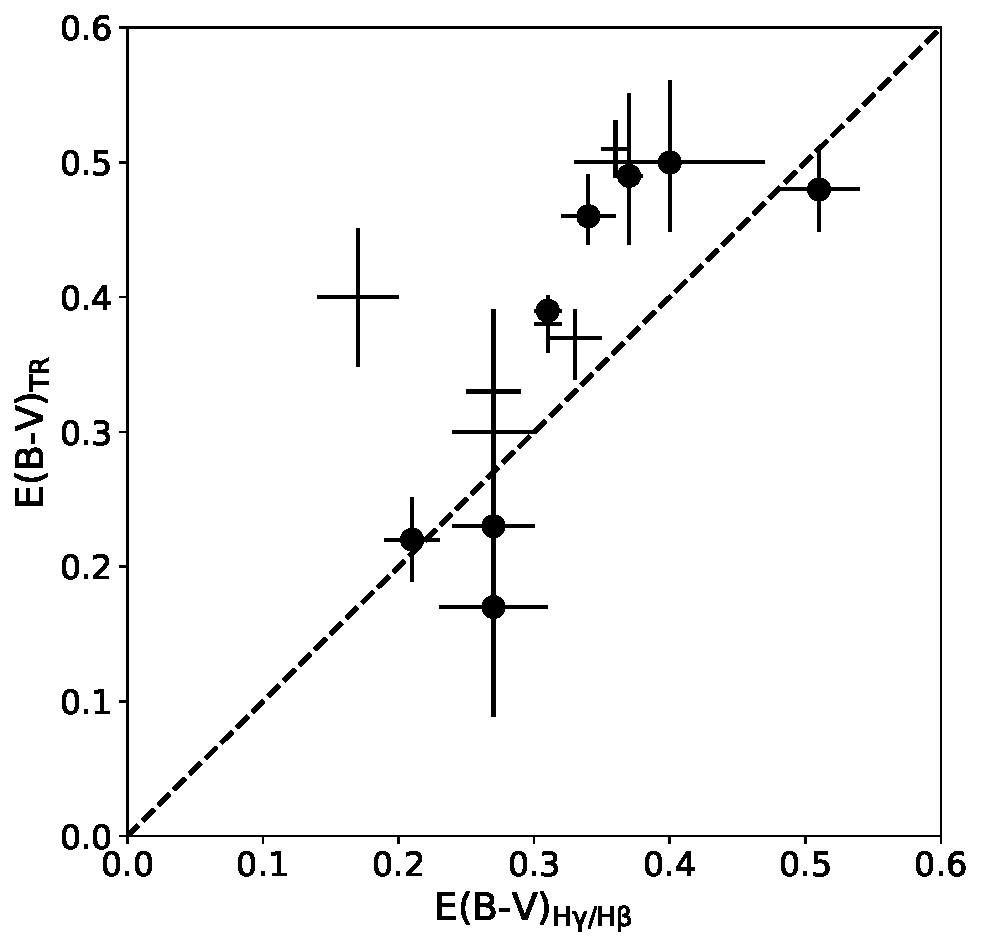
\includegraphics[width=0.75\linewidth]{figures/xshooter_ic5063/tr_balmer_reddening.pdf}
	\caption[Reddening values derived from the Balmer decrement plotted against values measured using the transauroral line technique.]{Reddening values derived from the Balmer decrement against values measured using the TR ratios. The black points represent the values measured in the various apertures and components, with broad components indicated by circles and narrow components by crosses, while the black dashed line shows the one-to-one relation. }
	\label{fig: xshooter_ic5063: tr_balmer_reddening}
\end{figure} 

\subsubsection{Electron temperatures and gas ionisation mechanisms}
\label{section: xshooter_ic5063: properties_of_outflowing_gas: uvb_vis_analysis_and_results: electron_temperatures}

Emission lines resulting from forbidden transitions of the O$^{+2}$ ion were used to determine electron temperatures --- this served as an initial probe of the ionisation mechanism of the outflowing and quiescent warm-ionised gas, since shock-ionised gas is expected to have a higher electron temperature than gas photoionised by AGN \citep{Fosbury1978, VillarMartin1999}. Note that the standard BPT diagrams were not used to investigate the ionisation mechanisms of the gas because the shock and photoionisation models overlap considerably in these diagrams (Section\;\ref{section: introduction: outflows: accleration_mechanisms: ionisation_and_excitation_mechanisms}, Figure\;\ref{fig: introduction: outflows: acceleration_mechanisms: bpt_diagram_photo_shock_ionisation}; \citealt{Zaurin2013}; \citealt{Santoro2018}), and the line profiles of H$\mathrm{\alpha}$ and the [NII]$\lambda\lambda$6548,6583 doublet are blended significantly in the apertures of interest. Electron temperatures were determined by using the extinction-corrected flux ratio [OIII](5007+4959)/4363 (using the [OIII] models to fit the lines) and transauroral-line-derived electron densities with the Lick Observatory \textsc{fivel} script. Values of electron temperature measured in this way for each kinematic component are presented in Table\;\ref{tab: xshooter_ic5063: temps}.

Using the [OIII](5007+4595)/4363 ratio, electron temperatures in the range \newline11500\;\textless\;$T_e$\;\textless\;14000\;K were found, with no clear distinction (\textgreater\;$3\sigma$) between broad and narrow components except in Aperture 3, in which the two narrow components present higher electron temperatures than the broad component.

	\begin{table}
	\def\arraystretch{1.5}
	\centering
	\begin{tabular}{cccc}
	Component & Distance (arcsec) & Distance (kpc) & Temperature (K) \\ \hline
	AP1 Narrow   & $-$4.72                                                       & $-$1.21                                                    & 11934$^{+169}_{-207}$                                     \\
		&	&	&	\\
	AP2 Narrow   & $-$3.44                                                       & $-$0.88                                                    & 13776$^{+145}_{-96}$                                      \\
	&	&	&	\\
	AP3 Narrow 1 & $-$1.84                                                       & $-$0.47                                                    & 14117$^{+350}_{-293}$                                     \\
	AP3 Narrow 2 & $-$1.84                                                       & $-$0.47                                                    & 13117$^{+185}_{-228}$                                     \\
	AP3 Broad    & $-$1.84                                                       & $-$0.47                                                    & 11564$^{+204}_{-160}$                                     \\
	&	&	&	\\
	AP4 Total    & 0                                                           & 0                                                        & 12578$^{+44}_{-44}$                                       \\
	&	&	&	\\
	AP5 Total    & 1.24                                                        & 0.32                                                     & 11810$^{+208}_{-164}$                                     \\
	&	&	&	\\
	AP6 Narrow   & 2.08                                                        & 0.53                                                     & 13921$^{+802}_{-666}$                                     \\
	AP6 Broad    & 2.08                                                        & 0.53                                                     & 12980$^{+941}_{-664}$                                     \\
	&	&	&	\\
	AP7 Narrow   & 3.04                                                        & 0.78                                                     & 11646$^{+457}_{-401}$                                     \\
	AP7 Broad    & 3.04                                                        & 0.78                                                     & 13680$^{+586}_{-517}$                                     \\
	&	&	&	\\
	AP8 Narrow   & 4.48                                                        & 1.15                                                     & 13537$^{+287}_{-282}$                                     \\ 
	\end{tabular}
	\caption[Electron temperatures for the warm ionised gas along the radio axis of IC\;5063, measured using the {[}OIII{]}(5007+4959)/4363 line ratio.]{Electron temperatures of the gas for each component in each aperture, derived using the [OIII](5007+4959)/4363 line ratio. The distances for each aperture are the same as given in Table\;\ref{tab: xshooter_ic5063: kinematics}.}
	\label{tab: xshooter_ic5063: temps}
\end{table}

To facilitate further comparisons with AGN photoionisation and shock models, the [OIII](5007/4363) against HeII$\lambda$4686/H$\mathrm{\beta}$ diagnostic diagram was produced (Figure\;\ref{fig: xshooter_ic5063: heii_hbeta}). The advantage of this diagram is that, not only are the shock and AGN-photoionisation models more clearly separated than in BPT diagrams, but it allows determinations of the extent to which the presence of matter-bounded clouds may play a role \citep{VillarMartin1999}. The AGN-photoionisation models were those generated by \textsc{Cloudy}, as described in Section\;\ref{section: xshooter_ic5063: properties_of_outflowing_gas: uvb_vis_analysis_and_results: transauroral_lines}, for a radiation-bounded, solar-composition (1\;Z$_\odot$), dust-free gas with an electron density of $n_\mathrm{e}=10^3$\;cm$^{-3}$ (based on the densities derived using the TR ratios) and a central ionising continuum that follows a power law of shape $F_\mathrm{v}$ $\propto$ $v^{-1.5}$. Note that the [OIII](5007/4363) and HeII4686/H$\mathrm{\beta}$ ratios depend on these parameters --- the effects of varying them are quantified and discussed in \mbox{Appendix \ref{appendix: heii_hb_oiii_photoionisation_modelling}}. The solar-composition shock models were taken from the library presented by \citet{Allen2008}, which was created using the \textsc{Mappings III} code. In \mbox{Figure\;\ref{fig: xshooter_ic5063: heii_hbeta}}, measured line ratios are plotted on this diagram for each aperture in which outflows are detected, along with the modelled \textsc{Cloudy} ratios for different ionisation parameters (in the range \mbox{$-$3.0\;\textless\;log$U$\;\textless\;$-$1.5}), and the pre-shock (precursor) and post-shock (pure-shock) models from \textsc{Mappings III} for a pre-shock gas density of 100\;cm$^{-3}$, magnetic fields of 1, 10 and 100\;$\mathrm{{\mu}G}$, and different shock velocities (ranging from 100--1000\;km\;s$^{-1}$).

By comparing the measured line ratios to those from the AGN-photoionisation and shock models, it can be seen that AGN photoionisation is dominant for both the outflowing and non-outflowing gas along the radio axis of IC\;5063. I highlight that, while pure AGN photoionisation requires a sub-solar metallicity ($\sim$0.5\;Z$_\odot$) and higher ionisation parameters than are measured here to explain some of the measured ratios, a different assumed spectral index would also help improve consistency with the AGN photoionisation models (see Appendix \ref{appendix: heii_hb_oiii_photoionisation_modelling}). Therefore, a plausible combination of these parameters exists that produces line ratios consistent with the measurements presented here. While some contribution from shocks cannot be ruled out, it should be noted that the [OIII](5007/4363) and HeII$\lambda$4686/H$\mathrm{\beta}$ ratios do not discriminate between broad and narrow components in this case (unlike the case presented by \citealt{VillarMartin1999}). Therefore, this is taken as evidence that both the quiescent and outflowing gas in the warm ionised phase are predominantly AGN-photoionised.

Moreover, moderate ($\sim0.10$--0.25) HeII$\lambda$4686/H$\mathrm{\beta}$ ratios and low-to-moderate [OIII] temperatures (\mbox{60\;\textless\;[OIII](5007/4363)\;\textless\;120}; 11500\;\textless\;$T$\;\textless\;14200\;K) are found for all components, both narrow and broad. These ratios rule out a major contribution from matter-bounded components \citep{Binette1996}.

\begin{figure}[!ht]
	\centering
	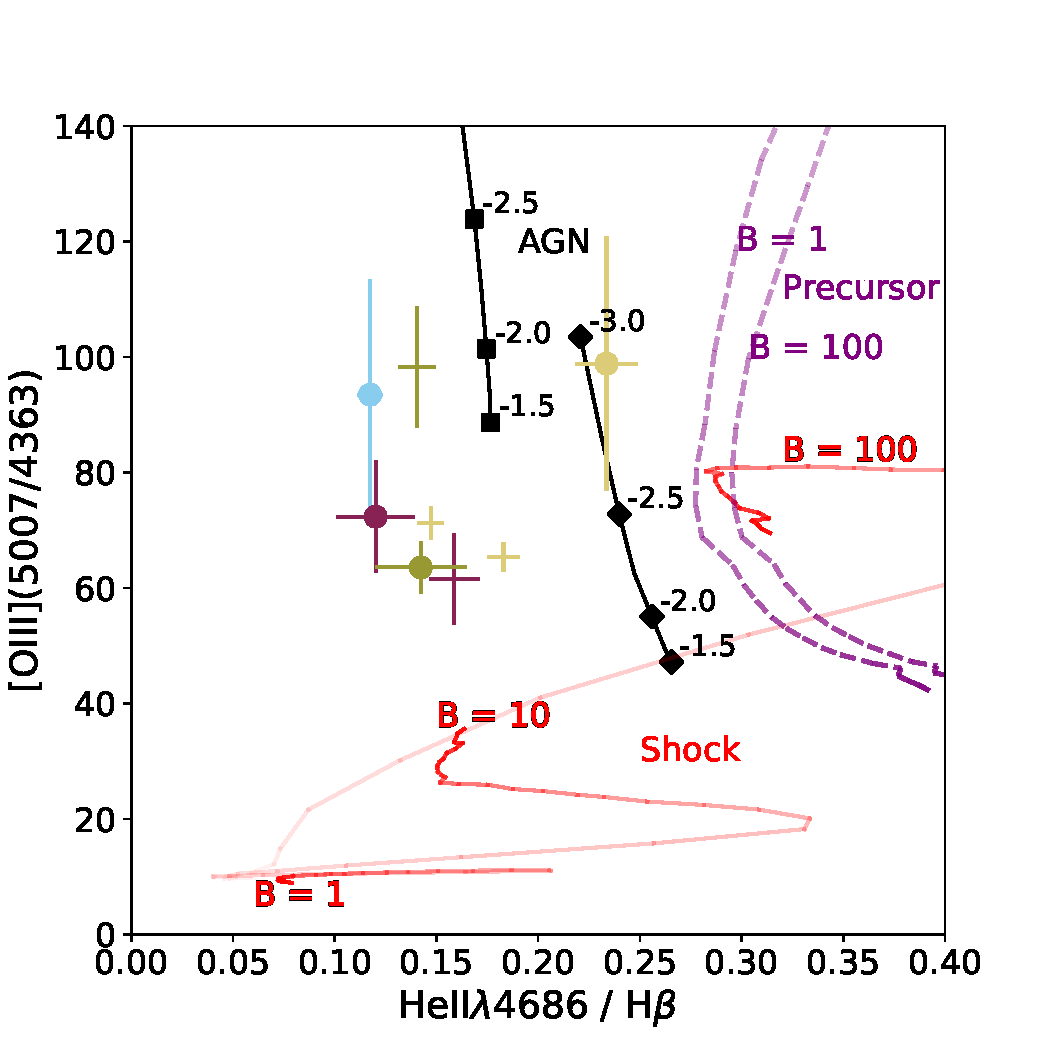
\includegraphics[width=0.7\linewidth]{figures/xshooter_ic5063/L_1Z.pdf}
	\caption[HeII$\lambda$4686/H$\mathrm{\beta}$ vs {[}OIII{]}(5007/4363) diagnostic diagram for the warm ionised gas in IC\;5063, including predicted values for photo- and shock-ionised gas.]{Measured HeII$\lambda$4686/H$\mathrm{\beta}$ and [OIII](5007/4363) line ratios for the outflowing gas in the Xshooter apertures --- the colour and marker scheme for each aperture is the same as in Figure\;\ref{fig: xshooter_ic5063: tr_grid}. Also plotted are AGN photoionisation models (black markers and lines) for different ionisation parameters (labelled) and spectral indices (squares: $\mathrm{\alpha}=1.5$; diamonds: $\mathrm{\alpha}=1.0$) of solar composition (1\;Z$_\odot$) gas of density $n_\mathrm{e}=10^3$\;cm$^{-3}$. Line ratios produced by shock-ionisation models taken from the \textsc{Mappings III} library presented by \citet{Allen2008} for gas with a pre-shock electron density of 100\;cm$^{-3}$, magnetic fields of 1, 10 and 100\;$\mu G$, and shock velocities ranging from 100--1000\;km\;s$^{-1}$ are shown as purple dashed lines (pre-shock/precursor gas) and red solid lines (post-shock gas). Lower shock velocities are shown with fainter lines, and higher shock velocities are shown with darker lines.}
	\label{fig: xshooter_ic5063: heii_hbeta}
\end{figure}

\subsubsection{Mass outflow rates and kinetic powers}
\label{section: xshooter_ic5063: properties_of_outflowing_gas: uvb_vis_analysis_and_results: energetics}

In order to facilitate comparisons between the results presented here, models of galaxy evolution, and previous observations of the different gas phases in IC\;5063, the derived properties of the outflows at different positions were used to derive mass outflow rates, kinetic powers, and coupling efficiencies for the warm-ionised outflows along the radio axis of IC\;5063.

The luminosities of the H$\mathrm{\beta}$ line for the broad component in each aperture were first calculated using
\begin{equation}
L(\mathrm{H\beta}) = F(\mathrm{H\beta})\times 4\pi D^2_L,
\end{equation}
where F(H$\mathrm{\beta}$) is the reddening-corrected flux of the H$\mathrm{\beta}$ line (measured from Gaussian fits using the [OIII] models), and $D_\mathrm{L}$ is the luminosity distance of IC\;5063. 

These luminosities were then used to determine the mass of an outflow in a given aperture using Equation \ref{eq: introduction: outflows: energetics: mout} with an assumed Case B recombination coefficient of $\alpha^\mathrm{eff}_\mathrm{H\beta}=3.03\times10^{-14}$\;cm$^{-3}$ (for $n_e=10^4$\;cm$^{-3}$ and $T_e=10^4$\;K) and electron densities derived from the TR ratios. Subsequently, the outflow masses derived in this way were used to produce mass outflow rate estimates for each aperture using Equation \ref{eq: introduction: outflows: energetics: mout_rate}, where $\Delta{R}$ was taken to be the width of a given aperture, and planar outflow geometry was assumed ($A=1$). As discussed in Section\;\ref{section: xshooter_ic5063: properties_of_outflowing_gas: uvb_vis_analysis_and_results: kinematics}, the outflow velocities ($v_\mathrm{out}$) were taken to be the difference between the percentile velocity ($v_\mathrm{p}$) of the broad component and the flux-weighted velocity ($v_\mathrm{w}$) of the narrow component in a given aperture (Table\;\ref{tab: xshooter_ic5063: kinematics}). 

Kinetic powers were estimated by using these mass outflow rates and kinematics with Equation\;\ref{eq: introduction: outflows: energetics: ekin}. I note that, since the outflow velocities were determined using percentile velocities (and it was assumed that the extremities of the emission-line wings represent the highest velocities along the LOS), the velocity width term of Equation\;\ref{eq: introduction: outflows: energetics: ekin} was not used (i.e. $\sigma$ was set to be zero). Finally, the resulting outflow kinetic powers were then compared to AGN bolometric luminosity to give coupling efficiencies ($\epsilon_\mathrm{f}$) using Equation\;\ref{eq: introduction: outflows: introduction: e_f}; the bolometric luminosity of IC\;5063 was taken to be 7.6$\times 10^{44}$\;erg\;s$^{-1}$ \citep{Nicastro2003, Morganti2007}. The resulting coupling efficiencies are presented in Figure\;\ref{fig: xshooter_ic5063: fkin} and Table\;\ref{tab: xshooter_ic5063: mout_fkin}. 

Low mass outflow rates (\mbox{\textless\;0.2\;M$_\odot$\;yr$^{-1}$}) and coupling efficiencies (\mbox{$\ll$\;0.5 per cent}) are found in all apertures --- much lower than those previously derived in some observational studies of samples of AGN (e.g. $\dot{M}_\mathrm{out}\sim10$--10,000\;M$_\odot$yr$^{-1}$: \citealt{Fiore2017}) and those required in galaxy-evolution models ($\epsilon_\mathrm{f}\sim0.5$--10\;per\;cent: e.g. \citealt{DiMatteo2005, Hopkins2010}). Furthermore, another set of coupling efficiencies was calculated (labelled $\epsilon_\mathrm{f}^{\prime}$) by determining the ratio of outflow kinetic power to the minimal jet power used in modelling of the jet-ISM interactions in IC\;5063 (P$_\mathrm{jet}$ = 10$^{44}$\;erg\;s$^{-1}$: \citealt{Mukherjee2018}). From this comparison, low values of $\epsilon_\mathrm{f}^{\prime}$ (\mbox{\textless\;0.001 per cent}) were produced, indicating that the kinetic power of the outflows accounts for an extremely small fraction of the total jet power and thus demonstrating the feasibility of jet-ISM interactions being the outflow acceleration mechanism.

\begin{figure}
	\centering
	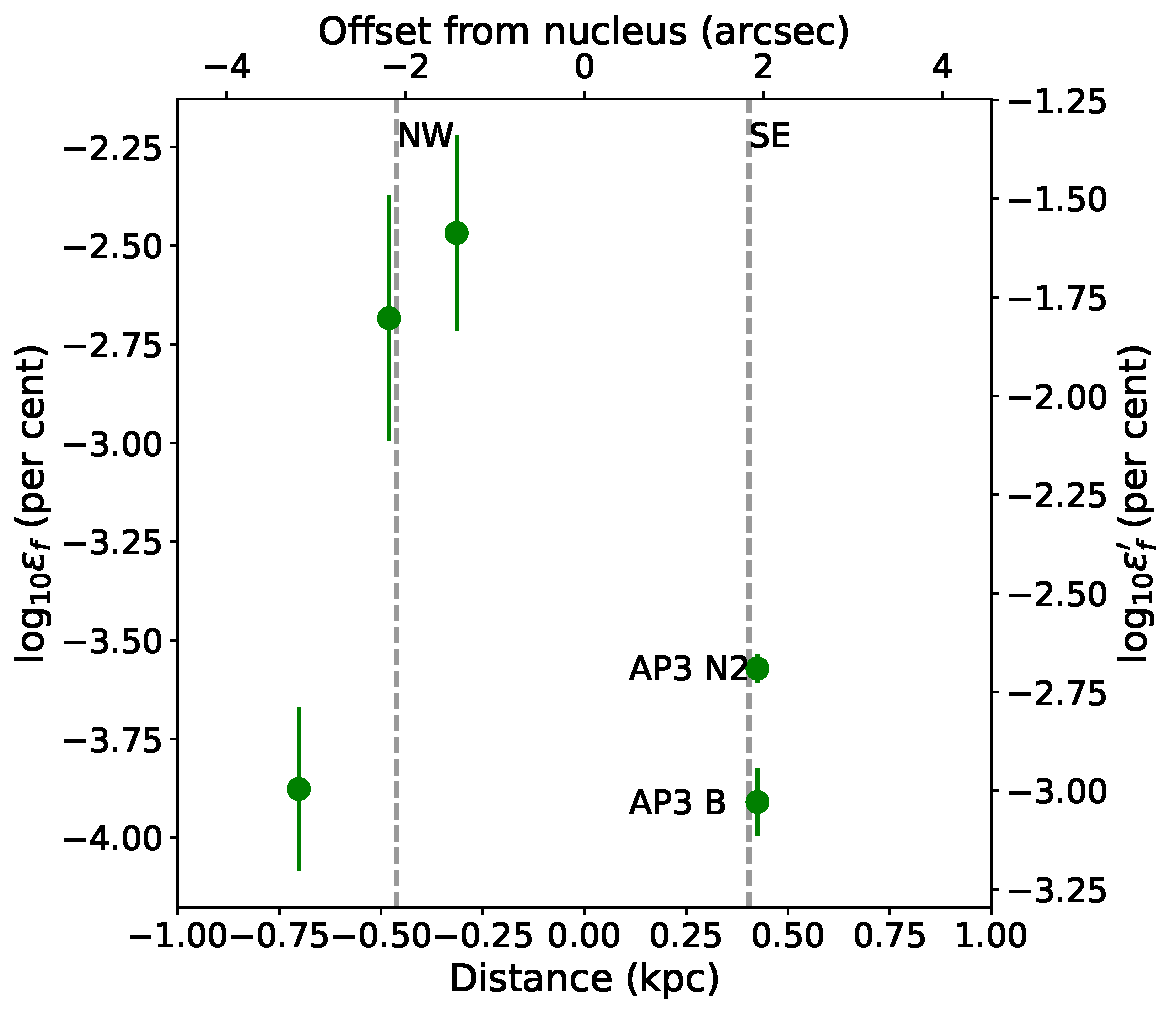
\includegraphics[width=0.8\linewidth]{figures/xshooter_ic5063/fkin.pdf}
	\caption[Outflow coupling efficiencies for the Xshooter apertures of IC\;5063, calculated for two cases: using the AGN bolometric luminosity, and for a jet of power $P_\mathrm{jet}=10^{44}$\;erg\;s$^{-1}$]{Percentage outflow coupling efficiencies in each aperture, calculated for two cases: using the nuclear bolometric luminosity of IC\;5063 given by \citet{Nicastro2003} and \citet{Morganti2007} ($\epsilon_\mathrm{f}=7.6\times 10^{44}$\;erg\;s$^{-1}$: left y-axis), and in the case that a jet of power P$_\mathrm{jet}=10^{44}$\;erg\;s$^{-1}$ \citep{Mukherjee2018} is the main driving mechanism ($\epsilon_\mathrm{f}^\prime$: right y-axis). The vertical dashed lines follow the same convention as Figure\;\ref{fig: xshooter_ic5063: velocities}, and the two kinematically-blueshifted components found in Aperture 3 (AP3 Broad and AP3 Narrow 2) are labelled.}
	\label{fig: xshooter_ic5063: fkin}
\end{figure}

\begin{table*}[!t]
	\renewcommand{\arraystretch}{1.5}
	\begin{tabular}{lcccc}
	Component    & $\dot{M}_\mathrm{out}$ (M$_\odot$yr$^{-1}$) & $\dot{E}_\mathrm{kin}$ (erg\;s$^{-1}$) & $\epsilon_\mathrm{f}$ (per cent) & $\epsilon_\mathrm{f}^\prime$ (per cent) \\ \hline
	AP3 Narrow 2 & 1.2$\pm$0.1 $\times 10^{-1}$              & 2.0$\pm$0.2 $\times10^{39}$  & 2.7$\pm$0.2 $\times 10^{-4}$   & 2.0$\pm$0.2 $\times 10^{-3}$          \\
	AP3 Broad    & 2.6$\pm$0.4 $\times10^{-2}$               & 9.4$\pm$1.8 $\times10^{38}$  & 1.2$\pm$0.2 $\times 10^{-4}$   & 9.4$\pm$1.8 $\times 10^{-4}$          \\ 
	AP5 Total    & 1.7$\pm$0.5 $\times 10^{-1}$               & 2.6$\pm$4.3 $\times10^{40}$  & 3.4$\pm$1.9 $\times 10^{-3}$   & 2.6$\pm$1.5 $\times 10^{-2}$          \\ 
	AP6 Broad    & 1.8$\pm$0.7 $\times 10^{-1}$              & 1.6$\pm$1.1 $\times10^{40}$  & 2.1$\pm$1.5 $\times 10^{-3}$   & 1.6$\pm$1.2 $\times 10^{-2}$          \\ 
	AP7 Broad    & 1.5$\pm$0.5 $\times 10^{-2}$              & 1.0$\pm$0.5 $\times10^{39}$  & 1.3$\pm$0.6 $\times 10^{-4}$   & 1.0$\pm$0.5 $\times 10^{-3}$          \\
	\end{tabular}
	\caption[Energetics for the warm ionised outflows in IC\;5063.]{Mass outflow rates, kinetic powers, and coupling efficiencies for the kinematic components associated with an outflow. The coupling efficiencies presented here are calculated using the nuclear bolometric luminosity of IC\;5063 given by \citet{Nicastro2003} ($\epsilon_\mathrm{f}=7.6\times 10^{44}$\;erg\;s$^{-1}$ ), and for a jet power of P$_\mathrm{jet} = 10^{44}$\;erg\;s$^{-1}$ ($\epsilon^\prime_\mathrm{f}$) as used in modelling by \citet{Mukherjee2018}.}
	\label{tab: xshooter_ic5063: mout_fkin}
\end{table*}


\newpage
\subsection{Analysis of the NIR apertures}
\label{section: xshooter_ic5063: properties_of_outflowing_gas: nir_analysis_and_results}

In order to obtain independent information about the gas ionisation/excitation and, potentially, acceleration mechanisms, the NIR spectra of the Xshooter observations of IC\;5063 were analysed separately.

First, it was found that the [OIII] models (Section\;\ref{section: xshooter_ic_5063: observations_and_data_reduction: emission_line_fitting}) did not describe the NIR emission-line profiles well: in many cases, the profiles were visibly different to those found in the UVB and VIS arms. Moreover, lines corresponding to different ionisation states (e.g. [FeII] and Pa$\mathrm{\beta}$) had differing line profiles within a given aperture. Therefore, unlike the UVB+VIS data, a line-profile model based on a single prominent emission line was not defined. Instead, each emission line was fit independently, and (as was done for the UVB+VIS spectra) Gaussian components were grouped into `broad' (\mbox{FWHM\;\textgreater\;500\;km\;s$^{-1}$}) or `narrow' (\mbox{FWHM\;\textless\;200\;km\;s$^{-1}$}) based on their line widths. Using the Gaussian fits produced in this way, the properties of several key, prominent emission lines in the NIR spectra were measured, namely [FeII]$\lambda$12570, [FeII]$\lambda$16400, Pa$\beta$, Br$\gamma$ and HeI$\lambda$10830 --- which trace the warm ionised phase --- and H$_2$1--0S(1)$\lambda$21218, which traces the warm molecular phase.

\subsubsection{The warm molecular gas phase}
\label{section: xshooter_ic5063: properties_of_outflowing_gas: nir_analysis_and_results: warm_molecular}

The H$_2 \lambda$21218 emission line can be used to probe the warm molecular gas phase, and comparing its line profile to those of forbidden and recombination lines allows for an investigation of the different outflow phases present in each aperture \citep{Tadhunter2014}. Broad ($\mathrm{FWHM}\sim500$\;km\;s$^{-1}$) components are seen in the H$_2 \lambda$21218 profiles in all apertures where outflowing gas is detected in [OIII] emission (consistent with the NIR observations of \citealt{Tadhunter2014}). Interestingly, the blueshifted narrow component in Aperture 3 seen in the optical line profiles (`AP3 Narrow 2') is absent in the H$_2 \lambda$21218 line profile (Figure\;\ref{fig: xshooter_ic5063: ap3_oiii_h2}), although it is present in the [FeII] and NIR recombination line profiles. This indicates that excited warm-molecular gas is not kinematically associated with the blueshifted component in Aperture 3.

\begin{figure}[!ht]
	\centering
	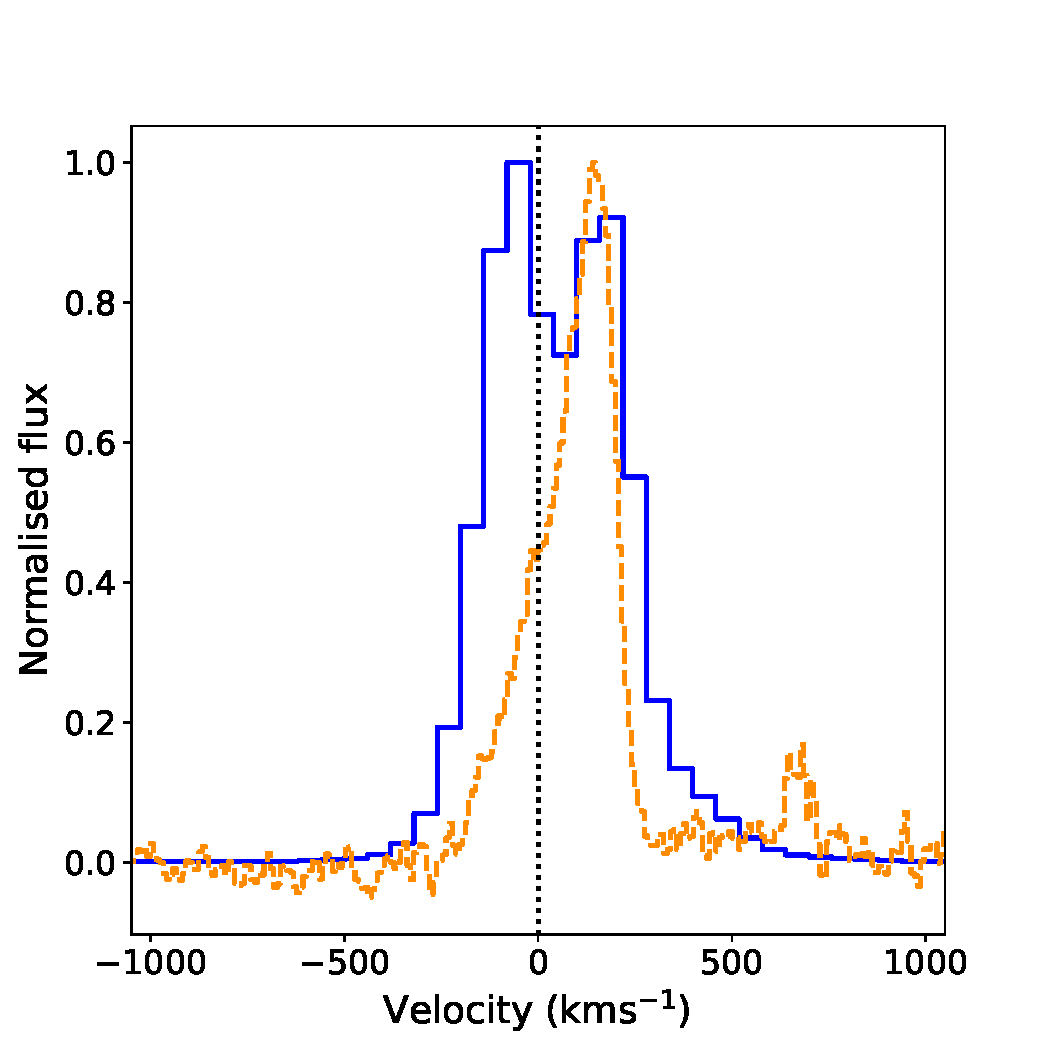
\includegraphics[width=0.7\linewidth]{figures/xshooter_ic5063/ap3_oiii_h2.pdf}
	\caption[Velocity profiles of for the {[}OIII{]}$\lambda$5007 and H$_2$1--0S(1)$\mathrm{\lambda}$21218 lines at the position of the SE radio lobe of IC\;5063.]{Velocity profiles for the [OIII]$\lambda$5007 (blue solid line) and \mbox{H$_2$1--0S(1)$\mathrm{\lambda}$21218} (orange dashed line) lines in Aperture 3. While a broad component --- representing outflowing gas --- is seen in both lines, the blueshifted narrow component seen in the [OIII] line profile (`AP3 Narrow 2'), emitted by the warm-ionised gas, is not present in the warm-molecular H$_2$ emission. Note that the [OIII]$\lambda$5007 line lies within the VIS Xshooter arm, and has been resampled to a wavelength step of 1\AA/pixel.}
	\label{fig: xshooter_ic5063: ap3_oiii_h2}
\end{figure}

\subsubsection{Ionisation and excitation of the near-infrared [FeII], Pa$\mathrm{\beta}$ and H$_2$ lines}
\label{section: xshooter_ic5063: properties_of_outflowing_gas: nir_analysis_and_results: excitation}

In order to supplement the investigation of the dominant outflow ionisation mechanism presented in Section\;\ref{section: xshooter_ic5063: properties_of_outflowing_gas: uvb_vis_analysis_and_results: electron_temperatures}, flux ratios of the [FeII]$\lambda$12570, [FeII]$\lambda$16400, and H$_2 \lambda$21218 emission lines and NIR recombination lines \citep{Rodriguez-Ardila2005, Riffel2013a, Colina2015, Riffel2021} were measured. In particular, I made use of the [FeII]$\lambda$12570/Pa$\mathrm{\beta}$ vs H$_2\lambda$21218/Br$\mathrm{\gamma}$ diagnostic diagram (see discussion in Section\;\ref{section: introduction: outflows: accleration_mechanisms: ionisation_and_excitation_mechanisms}) with the limits presented by \citet{Riffel2013a} and \citet{Riffel2021} that separate star-forming galaxies (SF), AGN and high line ratio (HLR) objects. The HLR region of the [FeII]$\lambda$12570/Pa$\mathrm{\beta}$ vs H$_2\lambda$21218/Br$\mathrm{\gamma}$ diagram contains objects such as Supernova Remnants (SNRs) and Low Ionisation Nuclear-Emission line Regions (LINERs; \citealt{Heckman1980}); objects for which photoionisation alone cannot explain the measured line ratios.

The line ratios of the different kinematic components in each aperture are shown plotted on this diagnostic diagram in Figure\;\ref{fig: xshooter_ic5063: feii_pab}, and are listed in Table\;\ref{tab: xshooter_ic5063: nir_ratios}. It is striking that the broad components of the NIR emission line profiles have higher H$_2\lambda$21218/Br$\mathrm{\gamma}$ ratios relative to the narrow components, with the broad components falling in the HLR region and the narrow components falling within the AGN region. Considering that the H$_2\lambda$21218/Br$\mathrm{\gamma}$ ratio probes the excitation of the warm-molecular gas, this indicates that the narrow components of this phase are predominately AGN-excited, while the broad components have composite shock-AGN excitation. In contrast, there is no clear difference in the [FeII]$\lambda$12570/Pa$\mathrm{\beta}$ ratios of the broad and narrow components, indicating that the quiescent and outflowing warm-ionised gas is predominantly AGN-photoionised (consistent with the results of Section\;\ref{section: xshooter_ic5063: properties_of_outflowing_gas: uvb_vis_analysis_and_results: electron_temperatures}).

\begin{figure}[!ht]
	\centering
	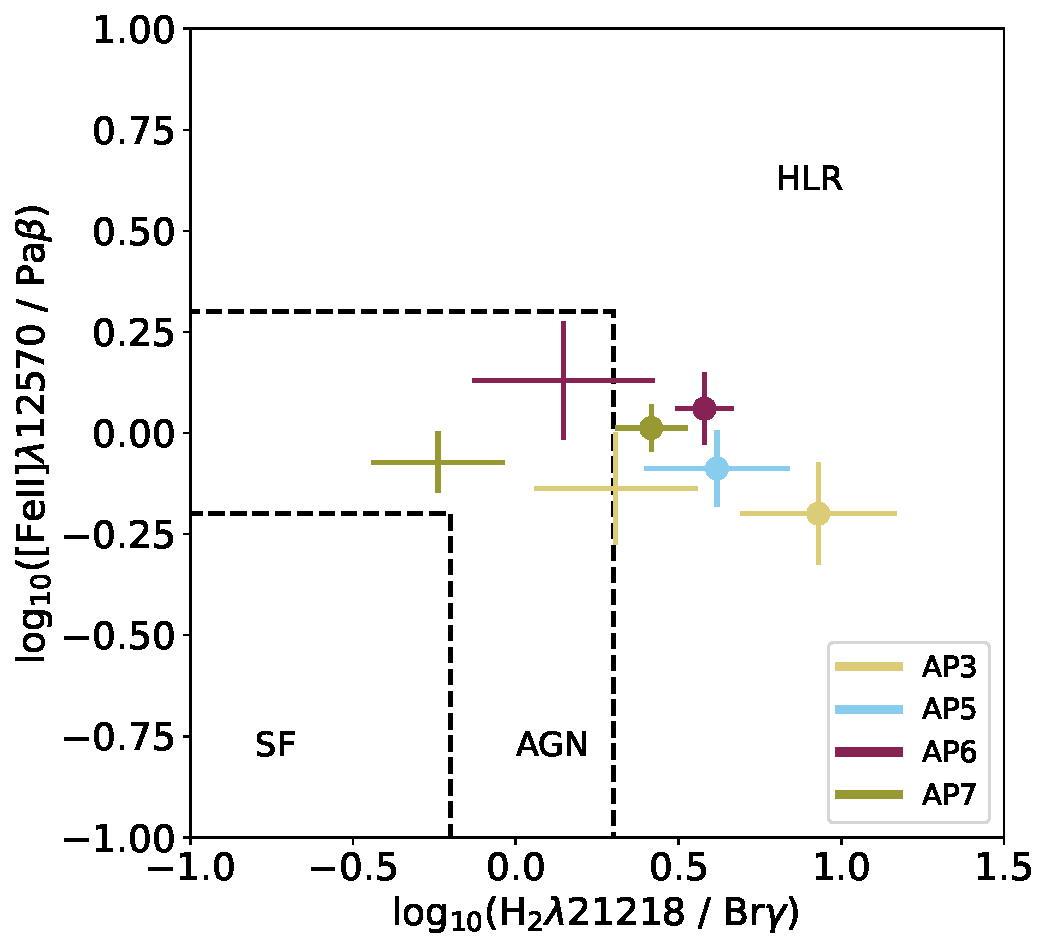
\includegraphics[width=0.75\linewidth]{figures/xshooter_ic5063/feii_pab.pdf}
	\caption[{[}FeII{]}$\lambda$12570/Pa$\mathrm{\beta}$ vs H$_2 \lambda$21218/Br$\mathrm{\gamma}$ NIR diagnostic diagram for the warm-ionised and warm-molecular NLR gas in IC\;5063.]{{[}FeII{]}$\lambda$12570/Pa$\mathrm{\beta}$ vs H$_2 \lambda$21218/Br$\mathrm{\gamma}$ NIR diagnostic diagram for the warm-ionised and warm-molecular NLR gas in IC\;5063 \mbox{(crosses: narrow components; circles: broad components)}, with regions defined by \citet{Riffel2021}: `SF' denotes observed line ratios which are associated with ionisation/excitation from star formation; `AGN' denotes line ratios which are associated with the central regions of AGN, and `HLR' denotes values higher than those observed from AGN-photoionisation/excitation alone. It has been proposed that line ratios in the HLR region indicate a contribution from shock-excitation, either from supernovae (SNe) or jet-ISM interactions. For IC\;5063, kinematic components associated with outflows fall within the HLR, with the quiescent components falling within the AGN region. The colour and marker scheme is the same as in Figure\;\ref{fig: xshooter_ic5063: tr_grid}.}
	\label{fig: xshooter_ic5063: feii_pab}
\end{figure}

\begin{table*}
	\centering
	\renewcommand{\arraystretch}{1.5}
	\begin{tabular}{lccc}
	Component    & H$_2\lambda$21218/Br$\mathrm{\gamma}$ & [FeII]$\lambda$12570/Pa$\mathrm{\beta}$ & [FeII]$\lambda$16400/Br$\mathrm{\gamma}$ \\ \hline
	AP3 Narrow 1 & 2.0$\pm$1.2    & 0.7$\pm$0.2                   & 4.5$\pm$2.5                  \\
	AP3 Broad    & 8.5$\pm$4.7    & 0.6$\pm$0.2                   & 3.1$\pm$1.8                  \\
		&	&	&	\\
	AP5 Total    & 4.2$\pm$2.1    & 0.8$\pm$0.2                   & 5.8$\pm$3.2                  \\
	&	&	&	\\
	AP6 Narrow   & 1.4$\pm$0.9    & 1.4$\pm$0.5                   & 3.6$\pm$2.2                  \\
	AP6 Broad    & 3.8$\pm$0.8    & 1.2$\pm$0.2                   & 6.5$\pm$1.6                  \\
	&	&	&	\\
	AP7 Narrow   & 0.6$\pm$0.3    & 0.9$\pm$0.2                   & 5.3$\pm$1.3                  \\ 
	AP7 Broad    & 2.6$\pm$0.7    & 1.0$\pm$0.1                   & 4.1$\pm$1.2                  \\
	\end{tabular}
	\caption[Ratios of NIR H$_2$ and {[}FeII{]} emission lines to recombination lines for the outflows in IC\;5063.]{Ratios of NIR H$_2$ and [FeII] emission lines to recombination lines for the components that are taken to represent outflowing gas. These values are shown on the [FeII]$\lambda$12570/Pa$\mathrm{\beta}$ vs H$_2\lambda$21218/Br$\mathrm{\gamma}$  diagnostic plot in Figure\;\ref{fig: xshooter_ic5063: feii_pab}, which is used to investigate the excitation mechanisms of the outflowing gas.}
	\label{tab: xshooter_ic5063: nir_ratios}
\end{table*}


\clearpage
\section{Discussion}
\label{section: xshooter_ic5063: discussion}

The results presented in Section\;\ref{section: xshooter_ic5063: properties_of_outflowing_gas} provide evidence for outflowing gas at the NW and SE radio lobes of IC\;5063 --- driven by jet-ISM interactions --- in agreement with the findings of previous studies (e.g. \citealt{Morganti2007, Tadhunter2014, Morganti2015}). This section discusses the relationship between the different gas phases at the NW lobe in detail, investigates which outflow phase is dominant in terms of mass and kinetic power through comparison to previous observations, and proposes a physical relation between the different gas phases and components along the radio axis. Finally, the implications of these findings for the transauroral-line technique of deriving electron densities are discussed.

\subsection{Placing the warm-ionised outflows at the NW lobe in a multi-phase context}
\label{section: xshooter_ic5063: discussion: multiphase}

\subsubsection{Kinematics of the different gas phases}
\label{section: xshooter_ic5063: discussion: multiphase: kinematics}

The [OIII] kinematics observed along the radio axis in IC\;5063 are consistent with a combination of regular gravitational disk rotation (traced by the narrow components, with the exception of the `Narrow 2' component in Aperture 3) and outflows of velocity 300\;\textless\;$v_\mathrm{out}$\;\textless\;700\;km\;s$^{-1}$ (traced by the broad components). As noted in previous work, the close association between highly-disturbed emission-line kinematics and the radio structure provides strong evidence that the warm-gas outflows are driven by the radio jet (e.g. \citealt{Morganti2007}, \citealt{Tadhunter2014}).

Kinematically, the results reported here for the warm ionised phase differ from what has previously been found for the cold-molecular gas. Here, extreme warm-ionised outflow kinematics are found at several positions along the radio axis, including the regions between the nucleus and the centroids of the radio lobes, whereas previous observations for the cold molecular phase --- as traced by CO emission lines --- find more extreme kinematics at the outer limit of NW lobe than elsewhere \citep{Morganti2015, Oosterloo2017}. In the two-dimensional Xshooter spectra for the warm-ionised gas (Figure\;\ref{fig: xshooter_ic5063: o2_pv_diagram}), there are indeed high-velocity blue wings extending to $v\sim1000$\;km\;s$^{-1}$ at the NW lobe, consistent with what is seen for the cold molecular phase. However, unlike the cold molecular phase, the warm-ionised gas profiles also have red wings extending to $v\sim800$\;km\;s$^{-1}$ at the position of the SE lobe. Most strikingly, the most extended velocity wings of the warm ionised phase, redshifted up to a maximum velocity of $\sim$1500\;km\;s$^{-1}$ at zero intensity, are found at a location \textit{between} the nucleus and the centroid of the NW lobe. The spatial centroid of this wing between \mbox{1000\;\textless\;$v$\;\textless\;1500\;km\;s$^{-1}$}, as measured by Gaussian fits to the continuum-subtracted spatial flux profile (as in Section\;\ref{section: xshooter_ic5063: properties_of_outflowing_gas: uvb_vis_analysis_and_results: spatial_distributions}) of the [NII]$\lambda$6583 line, lies 1.41\;arcsec northwest of the continuum centroid, or $\sim$0.6\;arcseconds (0.14\;kpc) closer to the nucleus than the centroid of the NW lobe.

The kinematics of the warm molecular phase, as traced with the H$_2\lambda$21218 emission, follow the warm-ionised kinematics. A blue velocity wing is seen to extend to $v\sim1000$\;km\;s$^{-1}$ at the centroid of the NW lobe, and a red wing extends to $v$\;\textgreater\;1000\;km\;s$^{-1}$ between this position and the nucleus (Figure\;\ref{fig: xshooter_ic5063: ap56_h2_velocity_profile}). This feature may extend to higher velocities, potentially up to $v\sim1500$\;km\;s$^{-1}$ (as seen in the warm-ionised gas), but blending with the continuum makes it difficult to determine the true velocity extent. These observed H$_2\lambda$21218 kinematics are also consistent with previous observations of the warm molecular phase by \citet{Tadhunter2014}.

The kinematics observed in the warm ionised and molecular phases can be explained by an expanding hemispherical bow shock or bubble, the tip of which coincides with --- or extends slightly beyond --- the centroid of the NW lobe. Considering that this structure would be seen side-on, the highest velocity widths are expected closer to the nucleus than the centroid of the lobe due to projection effects (i.e. the gas moving along the observer's line of sight). This is consistent with the highest observed velocities being between the nucleus and the outer limit of the NW lobe. Likewise, lower projected velocities would be found at the centroid of the lobe (closer to the tip of the bow shock), as the outflowing gas there would be moving in a direction that is close to the plane of the sky. The Xshooter observations are also consistent with the kinematics seen in hydrodynamic modelling of IC\;5063 for a jet of power P$_\mathrm{jet}=10^{44-45}$\;erg\;s$^{-1}$ propagating through the disk, as presented by \citet{Mukherjee2018}, where red- and blue-shifted line wings are seen at all locations where the radio source is interacting with the ISM in the galaxy's disk.

\begin{figure*}[!p]
	\centering
	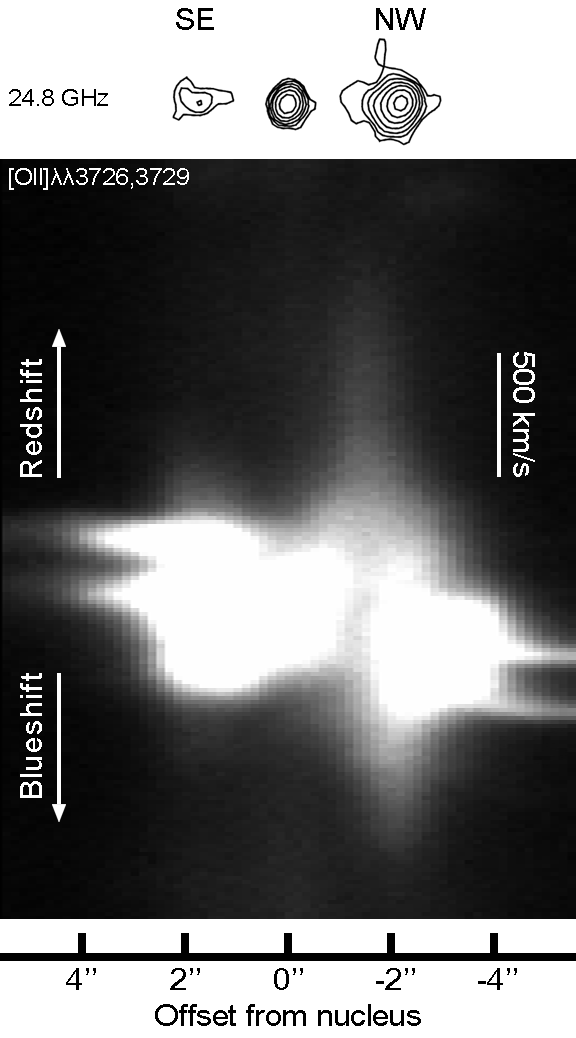
\includegraphics[width=0.7\linewidth]{figures/xshooter_ic5063/oii_h2_pv_diagram_3.png}
	\caption[Two-dimensional position-velocity profile of the {[}OII{]}$\lambda\lambda$3726,3729 doublet along the radio axis of IC\;5063, and corresponding 24.8\;GHz continuum contours.]{Two-dimensional position-velocity profile of the [OII]$\lambda\lambda$3726,3729 doublet. Here, the spatial direction is horizontal and the velocity (spectral) direction is vertical. Corresponding 24.8\;GHz continuum imaging by \citet{Morganti2007} is shown above the profile, indicating the shape and extent of the radio structure. The velocity scale bar represents a shift of $v=500$\;km\;s$^{-1}$. Very broad velocity wings can be seen at several locations, including at the centroids of the SE and NW lobes, with the most extended being a $v\sim1500$\;km\;s$^{-1}$ red wing between the nucleus and the centroid of the NW lobe.}
	\label{fig: xshooter_ic5063: o2_pv_diagram}
\end{figure*}

The difference in observed kinematics between the warm- and cold-molecular gas may be explained if the different molecular phases constitute a post-shock cooling sequence, as has been previously proposed to explain multi-phase outflow kinematics (see Section\;\ref{section: introduction: outflows: energetics: multi-phase}; \citealt{VillarMartin1999, Zubovas2014, Tadhunter2014}). In this scenario, the warm H$_2$ emission represents a transition phase, emitted as gas cools behind the shock through $T\sim2000$\;K, and has a constant mass and luminosity, assuming material passes through the shock at a constant rate. As the gas cools further, it enters the cold molecular phase, which emits the CO emission lines --- this represents the end-state of the cooling sequence. Assuming that the conditions for cold-molecular gas formation are met, and the molecular gas is not destroyed by AGN radiation, the ratio of cold-molecular gas (traced by CO emission) to warm-molecular gas (traced by H$_2$ emission) will thus increase as a function of time. In this scenario, if the gas seen in projection in-between the nucleus and the maximum extent of the NW radio lobe has only just started to enter the shock, it is plausible that not enough gas has yet accumulated in the cold molecular phase to be detectable via its CO emission. In contrast, gas may have been entering the shock at the tip of the hemispherical bow shock (the maximum extent of the NW lobe) for longer, allowing more time for CO-emitting cold-molecular gas to accumulate. This would explain why disturbed kinematics are seen at the centroid of the NW radio lobe for all phases, but only the warmer phases show more extreme kinematics in between this location and the nucleus.



\begin{figure}[!t]
	\centering
	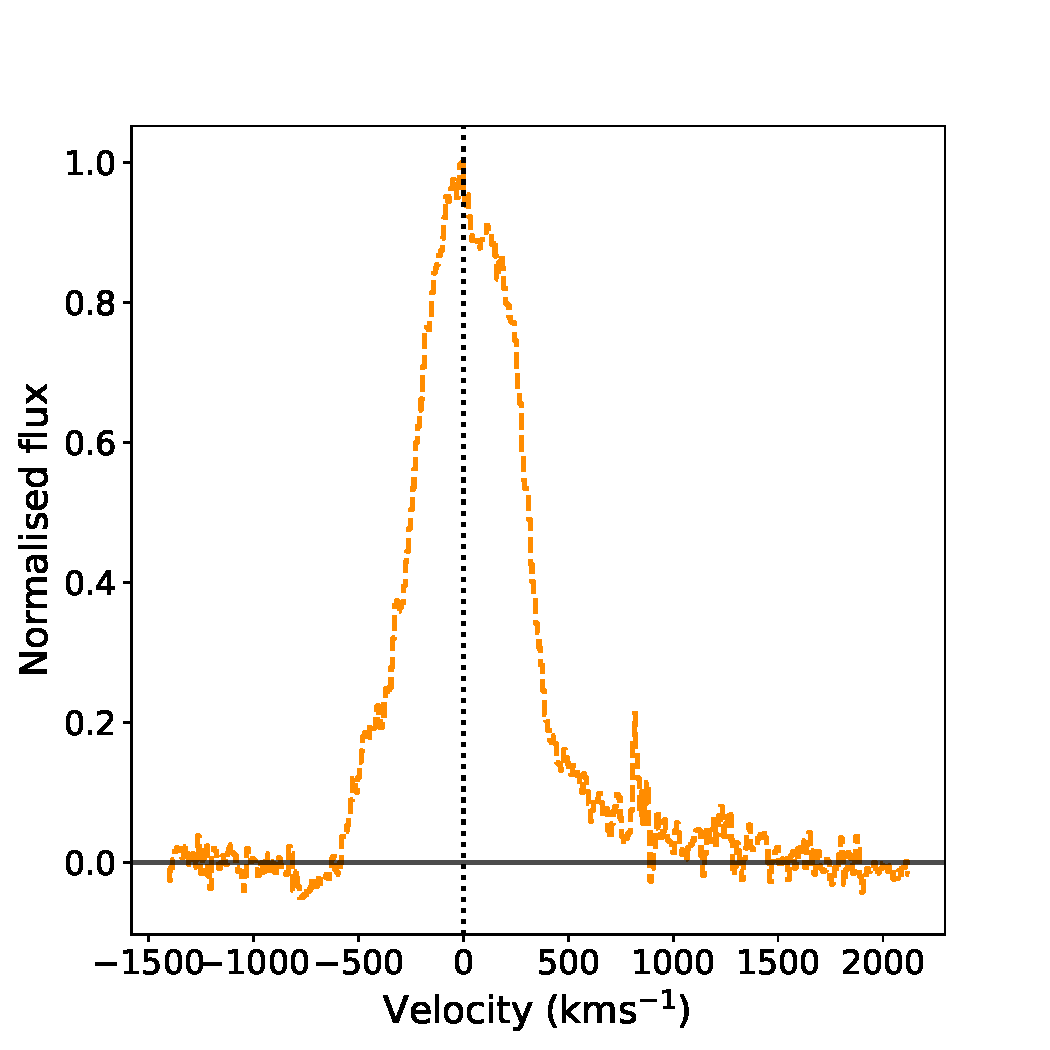
\includegraphics[width=0.7\linewidth]{figures/xshooter_ic5063/ap56_h2_velocity_profile.pdf}
	\caption[Velocity profile of the H$_2\lambda$21218 emission line at the location between the nucleus and outer extent of the NW radio lobe in IC\;5063.]{The velocity profile of the H$_2\lambda$21218 (dashed orange) line in the combined apertures 5 and 6, corresponding to the location between the nucleus and the outer extent of the NW radio lobe (Figure\;\ref{fig: xshooter_ic5063: apertures}). The dotted black vertical line represents a velocity of 0\;km\;s$^{-1}$, while the solid black horizontal line shows the continuum level. A red velocity wing extending to $v$\;\textgreater\;1000\;km\;s$^{-1}$ can be seen, consistent with the kinematics of the warm ionised phase (Figure\;\ref{fig: xshooter_ic5063: o2_pv_diagram}).}
	\label{fig: xshooter_ic5063: ap56_h2_velocity_profile}
\end{figure}

\subsubsection{Energetics of the multi-phase outflows}
\label{section: xshooter_ic5063: discussion: multiphase: energetics}

In order to ensure that the mass outflow rates and kinetic powers of the previously-observed neutral atomic and cold molecular phases are consistent with the results presented here for the warm ionised phase --- and to properly take into account results of the cold-molecular gas kinematics \citep{Morganti2015, Oosterloo2017} --- here, I recalculate values from past studies of IC\;5063 with a consistent methodology.

First, the mass outflow rate of the neutral-atomic (HI) outflow at IC\;5063's NW lobe was calculated using
\begin{equation}
    \dot{M}_\mathrm{out} = 30\cdot\frac{\Omega}{4\pi}\cdot\frac{r_\ast}{1\;\mathrm{kpc}}\cdot\frac{N_\mathrm{H}}{10^{21}\;\mathrm{cm}^{-2}}\cdot\frac{v_\mathrm{out}}{300}
\label{eq: xshooter_ic5063: appendix_hi_mout}
\end{equation}
from \citet{Morganti2005} (following the methodology given in \citealt{Heckman2002} and \citealt{Rupke2002}), where $N_\mathrm{H}$ is the column density of the gas and $\Omega$ is the solid angle through which the gas is flowing at a radius $r_\ast$ with a velocity of $v_\mathrm{out}$. Using the values and assumptions given in \citet{Morganti2005} --- namely that \mbox{$\Omega=\pi$}, \mbox{$r_\ast=0.4$\;kpc}, $N_\mathrm{H}=10\times10^{21}$\;cm$^{-2}$, and $v_\mathrm{out}=$ full width at zero intensity $\mathrm{(FWZI)}/2=350$\;km\;s$^{-1}$ --- a mass outflow rate of 35\;M$_\odot$\;yr$^{-1}$ was determined.

An important assumption made here is that the gas is outflowing through a solid angle of $\pi$, which is highly uncertain. Moreover, taking $v_\mathrm{out}$ = $\mathrm{FWZI}/2$ may underestimate the true outflow velocity in this case, since much of the blueshifted absorption in the HI 21\;cm profile of the NW lobe in IC\;5063 is concentrated close to the maximum blueshifted velocity (approximately $v=-700$\;km\;s$^{-1}$), in contrast to the other objects considered by \citet{Morganti2005}. Using $v_\mathrm{out}=700$\;km\;s$^{-1}$ rather than $v_\mathrm{out}=350$\;km\;s$^{-1}$ would result in a mass outflow rate that is a factor of two higher, and a coupling efficiency (see below) that is a factor of eight higher.

Next, the kinetic power of the HI outflow was calculated using the relation from \citet{Morganti2015}:
\begin{equation}
    \dot{E}_\mathrm{kin} = \frac{1}{2}\dot{M}_\mathrm{out}\Bigl(v^2_\mathrm{out}+\frac{v^2_\mathrm{turb}}{5.5}\Bigr),
\label{eq: xshooter_ic5063: appendix_ekin}
\end{equation}
where $v^2_\mathrm{turb}$ is the velocity component representing the turbulence of the outflowing gas, taken in \citet{Morganti2015} to be the FWHM\footnote{Since the turbulence term in Equation\;\ref{eq: xshooter_ic5063: appendix_ekin} corresponds to the velocity dispersion ($\sigma$; see Equation\;\ref{eq: introduction: outflows: energetics: ekin}), it is required that the FWHM value taken by \citet{Morganti2015} is divided by a factor of 5.5 ($\sigma^2=(\mathrm{FWHM}/2.35)^2\approx\mathrm{FWHM}^2/5.5$).} of the CO(2-1) emission line that is associated with the outflow. Assuming that the CO and HI-emitting gas have similar kinematics, then $v_\mathrm{turb}=\mathrm{FWHM}=100$\;km\;s$^{-1}$ \citep{Morganti2015} is used along with the determined mass outflow rate calculated here ($\dot{M}_\mathrm{out}=35$\;M$_\odot$\;yr$^{-1}$) and the outflow velocity given by \citet{Morganti2005} ($v_\mathrm{out}=350$\;km\;s$^{-1}$) --- this results in a neutral HI outflow kinetic power of \mbox{E$_\mathrm{kin}=1.4\times10^{42}$\;erg\;s$^{-1}$}. Comparing this to the estimated nuclear bolometric luminosity of IC\;5063 (7.6$\times10^{44}$\;erg\;s$^{-1}$: \citealt{Nicastro2003, Morganti2007}) using Equation \ref{eq: introduction: outflows: introduction: e_f}, a coupling efficiency of $\epsilon_\mathrm{f}=0.18$\;per\;cent is estimated for the neutral HI outflow at the NW radio lobe of IC\;5063.

For the cold molecular phase, the estimated mass outflowing at the NW lobe was taken to be \mbox{M$_\mathrm{out}=1.3\times10^{6}$\;M$_\odot$} (\citealt{Oosterloo2017}; assuming optically thin gas, an excitation temperature of $T_\mathrm{ex}=29$\;K, and a CO-to-H$_\mathrm{2}$ mass-conversion factor of $\alpha_\mathrm{CO} =
0.25$\;K\;km\;s$^{-1}$\;pc$^2$); the mass outflow rate was then calculated using a modified version of the relation given by \citet{Oosterloo2017} that is consistent with the method used in this chapter for the warm-ionised gas\footnote{The factor of three used by \citet{Oosterloo2017} is not used in mass outflow rate calculations of the warm ionised phase in this work, as this factor accounts for a spherical outflow geometry, which is not assumed here.}
\begin{equation}
    \dot{M}_\mathrm{out}=\frac{v_\mathrm{out}M_\mathrm{out}}{R},
\end{equation}
where $R$ is the size of the outflow region. Taking $R=0.5$\;kpc, $v_\mathrm{out}=300$\;km\;s$^{-1}$ (as in \citealt{Oosterloo2017}) and \mbox{$M_\mathrm{out}=1.3\times10^{6}$\;M$_\odot$}, a mass outflow rate of \mbox{$\dot{M}_\mathrm{out}=0.79$\;M$_\odot$\;yr$^{-1}$} is found.

Taking \mbox{$\dot{M}_\mathrm{out}=0.79$\;M$_\odot$\;yr$^{-1}$}, $v_\mathrm{out}=300$\;km\;s$^{-1}$, and $v_\mathrm{turb}=\mathrm{FWHM}=100$\;km\;s$^{-1}$ \citep{Morganti2015}, Equation \ref{eq: xshooter_ic5063: appendix_ekin} thus gives a kinetic power of $2.3\times10^{40}$\;erg\;s$^{-1}$. Subsequently, Equation \ref{eq: introduction: outflows: introduction: e_f} was used to calculate the coupling efficiency of the cold molecular phase to be $\epsilon_\mathrm{f}=3.1\times10^{-3}$\;per\;cent.

The true mass of the cold-molecular outflow is uncertain, and the value calculated here is likely a lower limit: the calculated outflow mass would be higher if the gas is assumed to be optically thick instead of optically thin. Assuming instead the highest excitation temperature observed by \citet{Oosterloo2017} ($T_\mathrm{ex}\sim55$\;K) would approximately double the estimated mass, and uncertainties regarding separating the outflowing and non-outflowing mass may mean that the true gas mass is a factor of a few higher than calculated here (see \citealt{Oosterloo2017} for a detailed discussion).

Combining these results with those of the warm-ionised outflows presented in this chapter, outflow masses, mass outflow rates, and coupling efficiencies for the different outflow phases in IC\;5063 are presented in Table\;\ref{tab: xshooter_ic5063: all_phases}; all coupling efficiencies ($\epsilon_\mathrm{f}$) have been calculated assuming a bolometric luminosity of $L_\mathrm{bol}=7.6\times 10^{44}$\;erg\;s$^{-1}$ \citep{Nicastro2003, Morganti2007}. The mass outflow rate derived for the warm-ionised gas at the NW lobe is higher than that for the warm-ionised gas found by \citet{Morganti2007} ($\dot{M}_\mathrm{ion} \sim 0.08 $\;M$_\odot$\;yr$^{-1}$). This difference is likely due to the different outflow radii used: \citet{Morganti2007} used the distance of a given aperture from the nucleus ($R$) with Equation \ref{eq: introduction: outflows: energetics: mout_rate}, whereas here the aperture width ($\Delta R$) is instead used, which is smaller and thus produces higher outflow rates.

However, the derived mass outflow rates for the warm-ionised gas are still significantly lower than those of the neutral atomic ($\sim$35\;M$_{\odot}$\;yr$^{-1}$) and cold molecular ($\sim$0.8\;M$_{\odot}$\;yr$^{-1}$) phases. In addition, the coupling efficiency of the warm ionised phase (\mbox{$\epsilon_\mathrm{f}=(2.7\pm1.7)\times10^{-3}$\;per\;cent}) is much lower than that of the neutral atomic phase ($\epsilon_\mathrm{f}\approx0.2$\;per\;cent), but similar to that of the cold molecular phase ($\epsilon_\mathrm{f} \approx$ $3.1\times10^{-3}$\;per\;cent), although as stated above, this is likely to be a lower limit. Overall, the mass and kinetic-power budgets of the outflows are dominated by the neutral phase, with the warm-ionised and cold-molecular gas making relatively minor contributions.

\begin{sidewaystable}
	\renewcommand{\arraystretch}{1.5}
	\centering
	\begin{tabular}{cccccc}
	Phase          & Location        & $M$ ($M_\odot$)                                                   & $\dot{M}_\mathrm{out}$ ($M_\odot$\;yr$^{-1}$) & $\epsilon_\mathrm{f}$ (per cent)   & Reference                             \\ \hline
	Warm ionised   & NW Lobe         & ---                                                                & 0.08                                        & ---                                 & \citet{Morganti2007} \\
				& Galaxy-wide\;$^a$ & 1.5$^{+3.0}_{-0.9} \times 10^6$                                    & ---                                          & ---                                 & \citet{Venturi2021}  \\
				& NW Lobe\;$^b$     & (9.9$\pm0.1) \times 10^4$                                       & (1.8$\pm$0.6) $\times$ $10^{-1}$          & (2.7$\pm$1.7) $\times$ $10^{-3}$ & This work                             \\
				& SE Lobe\;$^c$     & (2.2$\pm0.3) \times 10^4$                                       & (2.6$\pm$0.4) $\times$ $10^{-2}$          & (1.2$\pm$0.2) $\times$ $10^{-4}$ & This work                             \\
		&	&	&	&	\\
	Neutral HI     & NW Lobe         & ---                                              & 3.5$\times10^1$                                          & 1.8$\times10^{-1}$                                  & \citet{Morganti2005}\;$^d$ \\ 
	&	&	&	&	\\
	Cold molecular & NW Lobe         & 1.3$\times$ $10^6$ & 7.9$\times10^{-1}$                                     & 3.1$\times10^{-3}$                          & \citet{Oosterloo2017}\;$^{d}$ \\ 
	&	&	&	&	\\
				&                 &                                                                   &                                             &                                    &                                      
	\end{tabular} \\
	$^a$For the gas with [OIII] W70 (85th minus 15th velocity percentile)\;\mbox{\textgreater\;300\;km\;s$^{-1}$} across all outflow regions. \\
	$^b$For the NW lobe, the outflow mass is the sum of the masses in apertures 5 and 6, whereas the mass outflow rate and coupling efficiency represent the average values for apertures 5 and 6 (see Table\;\ref{tab: xshooter_ic5063: mout_fkin}). \\
	$^c$Taken from the values for the broad component in Aperture 3. \\
	$^d$Values have been recalculated using consistent methodology with the values presented in \citet{Morganti2005} and \citet{Oosterloo2017}, and are likely to be lower limits. \\
	\caption[Masses, mass outflow rates, and coupling efficiencies for the various outflow phases in IC\;5063, calculated with consistent methodology.]{Masses, mass outflow rates, and coupling efficiencies (for the nuclear bolometric case; see Section\;\ref{section: xshooter_ic5063: properties_of_outflowing_gas: uvb_vis_analysis_and_results: energetics}) for the different outflow phases in IC\;5063, as reported in this work and recalculated using the results from previous observational studies.}
	\label{tab: xshooter_ic5063: all_phases}
\end{sidewaystable}


\subsection{Outflow acceleration and ionisation/excitation mechanisms in IC 5063}
\label{section: xshooter_ic5063: discussion: mechanisms}

\subsubsection{Ionisation and excitation of the warm gas}
\label{section: xshooter_ic5063: discussion: mechanisms: warm_gas}

If the outflows in IC\;5063 are both accelerated and ionised by shocks induced by jet-ISM interactions, then it might be expected that the broad kinematic components would have higher electron temperatures than the quiescent narrow components \citep{Fosbury1978, VillarMartin1999}. However, in this work, there is no clear evidence for higher electron temperatures associated with outflowing components (Table\;\ref{tab: xshooter_ic5063: temps}). Only Aperture\;3 shows a significant (\mbox{\textgreater\;3$\sigma$}) difference in temperature between kinematic components, with the broad component having a \textit{lower} (instead of a higher) electron temperature. Furthermore, the electron temperatures measured for all components --- probed with the [OIII](5007/4363) ratio --- are consistent with pure AGN-photoionisation (Figure\;\ref{fig: xshooter_ic5063: heii_hbeta}).

Further potential evidence regarding the natures of the ionisation/excitation mechanisms is provided by the [FeII]$\lambda$12570/Pa$\mathrm{\beta}$ vs H$_2 \lambda$21218/Br$\mathrm{\gamma}$ diagnostic diagram (Figure\;\ref{fig: xshooter_ic5063: feii_pab}). The two ratios used in this diagram each probe a different gas phase: warm ionised and warm molecular, respectively. It is interesting that the measured values of the [FeII]$\lambda$12570/Pa$\mathrm{\beta}$ ratio are similar for the broad and narrow components --- consistent with the [OIII](5007/4363) vs HeII4686/H$\mathrm{\beta}$ diagram (Figure\;\ref{fig: xshooter_ic5063: heii_hbeta}) --- indicating that both the quiescent and outflowing warm-ionised gas are predominantly AGN-photoionised (in agreement with the results of a previous investigation of the warm ionised-outflows in IC\;5063 by \citealt{Morganti2007}). However, the H$_2 \lambda$21218/Br$\mathrm{\gamma}$ ratios, probing the excitation of the warm molecular phase, present a clear difference between broad and narrow components. Along this ratio axis, the quiescent gas falls within the region of the diagnostic diagram where AGN-photoexcitation is thought to be dominant (with perhaps some contribution from shocks: see \citealt{Riffel2021}), whereas the outflowing gas falls within the HLR region, within which AGN-photoexcitation alone cannot account for the high line ratios.

\subsubsection{The physical relation between the different gas phases}
\label{section: xshooter_ic5063: discussion: mechanisms: physical_relation}

Taken together, this investigation into the ionisation and excitation of the UVB+VIS and NIR lines in IC\;5063 indicates that the quiescent and outflowing warm-ionised gas, along with the quiescent warm-molecular gas, are predominantly ionised/excited by the central AGN, while the outflowing warm-molecular gas has a significant contribution from shock excitation. This rules out the idea that only a post-shock cooling sequence is being observed: in such a scenario, all the warm-ionised and warm-molecular gas in the outflow would be ionised by (and accelerated close to) the shock front, and the cold-molecular gas would represent the post-shock gas further from the shock front (and closer to the central AGN) that has cooled through the sequence.

Rather, a potential explanation for these results is that the cooled, post-shock gas closest to the AGN is photoionised by the AGN, resulting in an additional warm-ionised component which has post-shock kinematics and densities while being predominantly AGN-photoionised. In this scenario, presented in Figure\;\ref{fig: xshooter_ic5063: cooling_sequence_schematic}, the post-shock cooled gas that is furthest from the shock front (and photoionised by the AGN) would shield the post-shock gas that is closer to the shock front. If this AGN-photoionised component had a higher luminosity than the immediate-post-shock warm-ionised gas, then it would contribute much more strongly to the emission-line ratios, leading to values consistent with AGN-photoionisation being observed. However, the warm molecular phase --- which is only found cooling behind the shock --- would show line ratios consistent with shock-excitation, in agreement with the ratios measured from the NIR data.

\begin{figure*}[!t]
    \centering
    \includegraphics[width=1\linewidth]{figures/xshooter_ic5063/cooling_sequence_schematic.png}
    \caption[A schematic for the post-shock cooling sequence that could explain the observed locations, kinematics, and conditions of the various gas phases in IC\;5063.]{A schematic showing a possible stratification in the emission regions that could explain both the measured emission-line ratios (Figures \ref{fig: xshooter_ic5063: heii_hbeta} and \ref{fig: xshooter_ic5063: feii_pab}) and the spatial distributions of the various emission lines (Figure\;\ref{fig: xshooter_ic5063: spatial_nir} and Table\;\ref{tab: xshooter_ic5063: spatial_nir}) in IC\;5063. The different phases (labelled) are shown as different coloured regions, and photoionising radiation is shown as black dashed lines. Note that this could represent the structure in individual clouds, or an ensemble of clouds. In this schematic, no attempt has been made to reflect the true relative sizes of the emission regions.}
    \label{fig: xshooter_ic5063: cooling_sequence_schematic}
\end{figure*}

To investigate this situation further, spatial flux profiles of the integrated \mbox{$-$600\;\;\textless\;$v$\;\textless\;$-$400\;km\;s$^{-1}$} wings of several emission lines present in the NIR apertures ([FeII]$\lambda$16400, [FeII]$\lambda$12570, H$_\mathrm{2}\lambda$21218, Pa$\mathrm{\beta}$ and HeI$\lambda$10830) were produced using the same method as in Section\;\ref{section: xshooter_ic5063: properties_of_outflowing_gas: uvb_vis_analysis_and_results: spatial_distributions}. Here, the [FeII], HeI and Pa$\mathrm{\beta}$ lines trace the warm ionised phase (however the [FeII] lines are expected to be particularly strong in regions associated with shocks: \citealt{Dors2012} and \citealt{Riffel2013a}), while H$_\mathrm{2}\lambda$21218 traces the warm molecular phase. The resulting plot is presented as Figure\;\ref{fig: xshooter_ic5063: spatial_nir}, which shows tentative evidence that the [FeII] emission peaks in flux the furthest away from the nucleus, the peak of H$_\mathrm{2}\lambda$21218 emission lies inward of the [FeII] peak, and the HeI and Pa$\mathrm{\beta}$ emission peaks are the closest to the nucleus. This is supported by the centroid positions obtained by fitting Gaussian profiles to the spatial profiles (Table\;\ref{tab: xshooter_ic5063: spatial_nir}).

Given that the NW lobe is considered to be the location of the strongest shocks, this evidence for stratification in the emission regions supports the geometry presented in Figure\;\ref{fig: xshooter_ic5063: cooling_sequence_schematic}: the [FeII] emission traces the warm-ionised gas near the shock front, the H$_\mathrm{2}\lambda$21218 traces post-shock gas that has cooled to the warm molecular phase, and the HeI and Pa$\mathrm{\beta}$ emission traces the inner-most (AGN-photoionised) warm-ionised component. However, note that the measured [FeII]/Pa$\mathrm{\beta}$ ratios (Figure\;\ref{fig: xshooter_ic5063: feii_pab}; Table\;\ref{tab: xshooter_ic5063: nir_ratios}) may not be consistent with this scenario: while the measured H$_\mathrm{2}\lambda21218$/Br$\mathrm{\gamma}$ ratios appear to be enhanced relative to what is expected from AGN-excitation, the [FeII]/Pa$\mathrm{\beta}$ ratios show no such relative enhancement. Further near-infrared observations of IC\;5063's NW lobe, taken with an IFU at a higher spatial resolution, are therefore needed to investigate this situation and verify the cooling-sequence scenario proposed here.

\begin{figure}[!t]
    \centering
    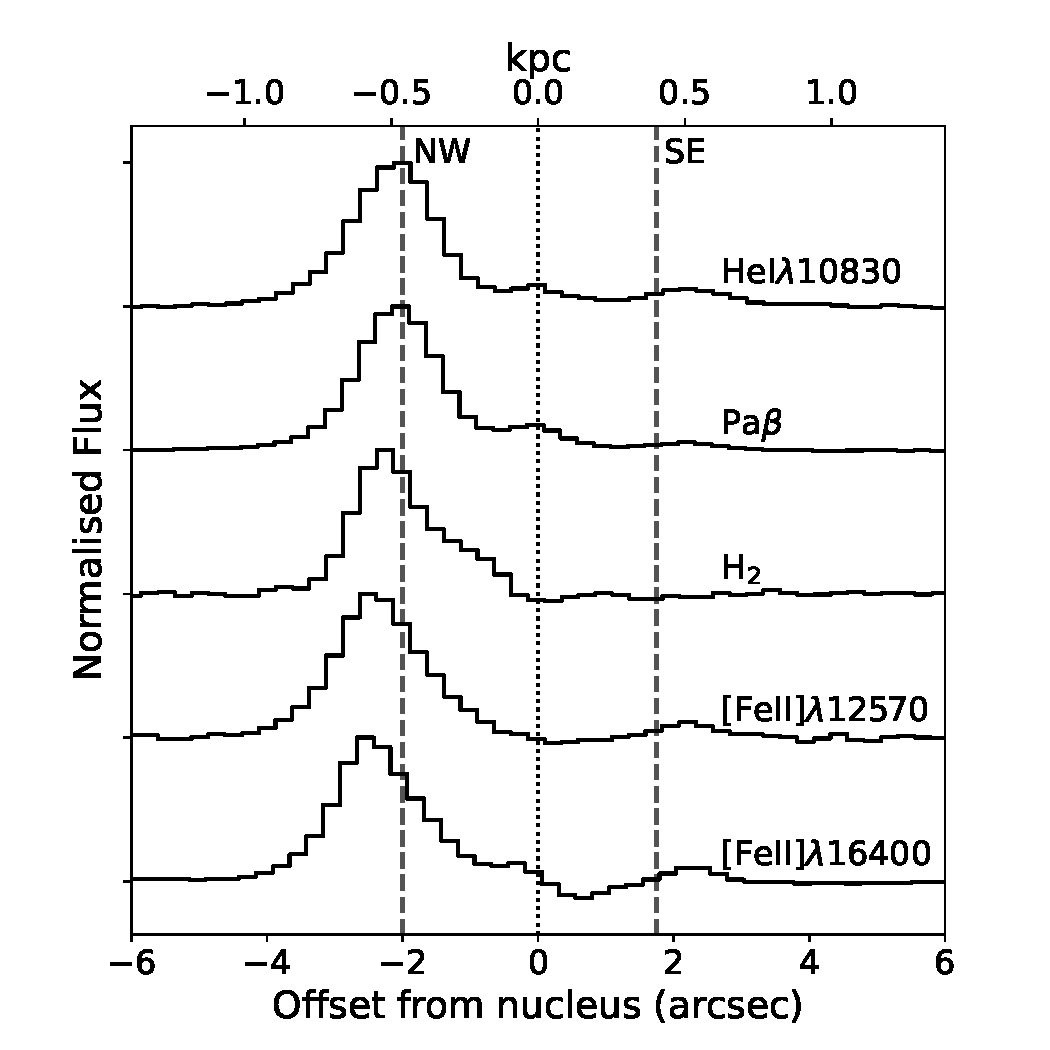
\includegraphics[width=0.7\linewidth]{figures/xshooter_ic5063/spatial_nir.pdf}
    \caption[Spatial flux distributions of the {[}FeII{]}$\lambda$16400, {[}FeII{]}$\lambda$12570, H$_\mathrm{2}\lambda$21218, Pa$\mathrm{\beta}$, and HeI$\lambda$10830 emission lines for the outflows in IC\;5063.]{Spatial flux distributions of the \mbox{$-$600\;\textless\;$v$ \;\textless\;$-$400\;km\;s$^{-1}$} wings of the emission-line profiles for [FeII]$\lambda$16400, [FeII]$\lambda$12570, H$_\mathrm{2}\lambda$21218, Pa$\mathrm{\beta}$, and HeI$\lambda$10830, produced using the same methodology as described in Section\;\ref{section: xshooter_ic5063: properties_of_outflowing_gas: uvb_vis_analysis_and_results: spatial_distributions}. It can be tentatively seen that the [FeII] lines (most likely tracing shocked warm-ionised emission) are emitted the furthest from the nucleus --- at the expected location of the shocks in the NW lobe --- with the warm-molecular H$_\mathrm{2}\lambda$21218 emission lying further inward, and the Pa$\mathrm{\beta}$ and HeI$\lambda$10830 emission lying closest to the nucleus. The centroids of Gaussian profiles fitted to these distributions are given in Table\;\ref{tab: xshooter_ic5063: spatial_nir}.}
    \label{fig: xshooter_ic5063: spatial_nir}
\end{figure}

\begin{table}[!t]
	\renewcommand{\arraystretch}{1.5}
    \centering
    \begin{tabular}{ccc}
    Emission Line           & Centroid (pixels) & Centroid (arcsec) \\ \hline
    HeI$\lambda$10830 & 8.5$\pm$0.2 & 2.11$\pm$0.05 \\
    Pa$\beta$ & 8.6$\pm$0.1 & 2.13$\pm$0.02 \\
    H$_\mathrm{2}\lambda$21218 & 9.5$\pm$0.1 & 2.36$\pm$0.02 \\
    {[FeII]$\lambda$12570} & 10.1$\pm$0.2 & 2.50$\pm$0.05 \\
    {[FeII]$\lambda$16400} & 10.2$\pm$0.2 & 2.53$\pm$0.05 \\                                                                                              
    \end{tabular}
    \caption[Measured centroids of Gaussian fits to the Spatial flux distributions of the {[}FeII{]}$\lambda$16400, {[}FeII{]}$\lambda$12570, H$_\mathrm{2}\lambda$21218, Pa$\mathrm{\beta}$, and HeI$\lambda$10830 emission lines for the outflows in IC\;5063.]{Centroids of Gaussian fits to spatial slices between \mbox{$-600$\;\textless\;$v$\;\textless\;$-400$\;km\;s$^{-1}$} of emission lines in the NIR arm data (Figure\;\ref{fig: xshooter_ic5063: spatial_nir}), measured relative to the spatial centroid position of the local continuum. The lines trace distinct phases of gas, which is interpreted here as a cooling sequence (Figure\;\ref{fig: xshooter_ic5063: cooling_sequence_schematic}).}
\label{tab: xshooter_ic5063: spatial_nir}
\end{table}

\subsubsection{Comparison to theoretical predictions of the dominant ionisation mechanism}
\label{section: xshooter_ic5063: discussion: mechanisms: model_comparison}

Relativistic hydrodynamic simulations by \citet{Meenakshi2022a} model the relative contribution of AGN-photoionisation and jet-induced-shock collisional-ionisation for a $5.71\times10^9$\;M$_\odot$ gas disk of radius 2\;kpc --- similar to the gas conditions and properties of IC\;5063 --- and find that shock-ionisation dominates the ionisation of the warm-ionised gas over AGN-photoionisation. This is inconsistent with the results presented here for IC\;5063, where AGN-photoionisation is found to be dominant. A potential reason for this discrepancy could be that the jet power in IC\;5063 is, in reality, an order of magnitude lower (P$_\mathrm{jet}$=10$^{44-45}$\;erg\;s$^{-1}$; \citealt{Mukherjee2018}) than assumed by \citet{Meenakshi2022a} (P$_\mathrm{jet}$=10$^{45}$\;erg\;s$^{-1}$). Moreover, the resolution of the simulations may not be sufficiently high to accurately track the density structure and cooling of the post-shock gas. Further simulation work that is more precisely tailored to the situation in IC\;5063 would allow this to be investigated in more detail, as would higher-resolution simulations of AGN and shock-ionisation for single clouds, which would allow a more accurate representation of the cooling of the warm gas.

\subsubsection{Compression effects of the jet-induced shocks}
\label{section: xshooter_ic5063: discussion: compression}

As the outflows along the radio-axis in IC\;5063 are likely to have been accelerated by jet-induced shocks, some evidence for shock-compression would be expected \citep{Sutherland2017}. Using the TR ratios (Section\;\ref{section: xshooter_ic5063: properties_of_outflowing_gas: uvb_vis_analysis_and_results: transauroral_lines}), it is found that the narrow components at all positions have relatively-low electron densities in the range \mbox{2.10\;\textless\;log$_{10}$(n$_e$[TR]\;cm$^{-3}$)\;\textless\;2.75}, while outflow components have significantly higher electron densities of \mbox{3.1\;\textless\;log$_{10}$(n$_e$[TR]\;cm$^{-3}$)\;\textless\;3.45}. This indicates that the outflows have higher electron densities than the quiescent gas by approximately a factor of three or four, possibly as a result of compression effects of the jet-induced shocks. This is similar to the findings of other AGN-driven-outflow studies, which find that broader components typically have higher densities \citep{Holt2011, Rose2018, Santoro2018, Santoro2020}, and is in line with what is expected for the immediate-post-shock gas due to the shock-jump conditions (a factor of four; \citealt{Sutherland2017}). However, the density contrast is much less than the factor of $\sim$100 which may be expected if the broad components originate from gas that has cooled in pressure equilibrium behind a fast shock \citep{Sutherland2017}.

\subsubsection{The nature of the blueshifted narrow [OIII] component seen in Aperture 3}
\label{section: xshooter_ic5063: discussion: ap3_narrow_component}

As seen in previous observations of the warm ionised phase of IC\;5063 \citep{Morganti2007}, a narrow kinematic component is identified at the position of the SE radio lobe that is blueshifted relative to the quiescent gas disk. Unlike the broad kinematic components associated with outflows, this component is narrow (\mbox{FWHM$_\mathrm{w}$\;\textless\;200\;km\;s$^{-1}$}) and has a lower electron density (log$_{10}n_\mathrm{e}=2.55\pm0.03$). Biconical outflows have been proposed to explain line splitting in active galaxies \citep{Walker1968, Cecil1990}, but if this is the case here, it is unclear why one direction of the outflow is broad and dense (AP3 Broad) and the other is narrow and has a lower density (AP3 Narrow 2). Alternatively, since IC\;5063 is thought to be a post-merger galaxy \citep{Morganti1998}, it would not be surprising to detect infalling and relatively-undisturbed low-density clumps of gas. Interestingly, H$_2$ emission that is kinematically associated with this component is not detected in Aperture\;3, implying that it either does not contain molecular gas or that the warm-molecular gas is not being excited. This is consistent with VLT/ISAAC observations presented by \citet{Tadhunter2014}, which show a blueshifted narrow component in the Br$\mathrm{\gamma}$ profile that is not present in the H$_2$1--0S(1) profile at the southeastern lobe. Furthermore, this component is not seen in cold-molecular PV diagrams (e.g. CO(1--0), CO(2--1), CO(3--2), HCO(4--3); \citealt{Morganti2015, Oosterloo2017}), implying a lack of cold-molecular gas. Therefore, infalling gas is the favoured explanation, and I propose that the situation for Aperture 3 is as follows: the broad component represents shock-accelerated outflowing gas, the red-most narrow component represents quiescent gas in IC\;5063's disk, and the blue-most narrow component represents infalling gas (that lacks molecular-gas emission) as a result of the recent merger.

\vfill

\subsection{The use of transauroral-line diagnostics in AGN-driven outflows}
\label{section: xshooter_ic5063: discussion: transauroral_lines}

This study marks the first time that the transauroral-line technique first presented by \citet{Holt2011} has been used to estimate electron density values for spatially-resolved outflow regions in an active galaxy. As previously discussed, a concern with this technique is that the transauroral [OII] and [SII] lines might be emitted by different clouds at different spatial positions to those emitting other important diagnostic lines. The work presented here shows that the transauroral lines have the same line profiles for the same kinematic components and are emitted at the same spatial positions as the high-ionisation optical forbidden and recombination lines (Figures \ref{fig: xshooter_ic5063: o3_models_all_lines} and \ref{fig: xshooter_ic5063: spatial_optical}), suggesting that they are emitted by the same cloud complexes. While it is not conclusively demonstrated in this work that the transauroral lines are emitted by the same clouds \textit{within} the apertures (see discussions in \citealt{Sun2017} and \citealt{Rose2018}), this does alleviate concerns regarding their use in spatially-unresolved studies of moderate-to-high redshift AGN.

In addition, the transauroral-line technique has been used alongside the traditional [OII] and [SII] line ratios and [ArIV] line ratio to show that this method gives electron densities that are slightly higher than (if not comparable to) those given by the traditional line ratios, but lower than those given by the [ArIV] ratio. \citet{Wang2004} found that the [ArIV] technique provides much higher electron densities in observations of ionised nebulae than the traditional ratios; the findings presented here support this and place the transauroral-line technique in between these two methods in terms of derived densities. 

Further detailed studies making use of the transauroral-line ratios alongside other methods of electron-density estimation are needed. However, this work highlights the necessity of careful consideration of the technique used to derive electron densities: the traditional [OII] and [SII] lines may underestimate the electron density of warm-ionised outflowing gas, while the [ArIV] ratio may overestimate it. This, in part, may be due to the [ArIV] ratio probing higher-ionisation gas than the traditional and transauroral [OII] and [SII] techniques. Since the [OIII] lines represent higher-ionisation gas than the [OII] and [SII] lines, then the findings reported here indicate that the density of the [OIII]-emitting gas may be higher than probed by the [OII] and [SII] lines. It is unclear how this relates to the density of the H$\mathrm{\beta}$-emitting gas, although it could mean that true mass outflow rates (thus kinetic powers and coupling efficiencies) are even lower than estimated here, and much lower than typically derived using densities estimated with the traditional [SII] and [OII] ratios. A more detailed investigation of this situation is undertaken in Chapter\;\ref{chapter: stis_seyferts}.

The high electron densities (\mbox{$n_e$\;\textgreater\;10$^3$\;cm$^{-3}$}) found for the outflowing components using the TR ratios are above those typically assumed by past studies for warm-ionised outflows in active galaxies (\mbox{10$^{2}$--$10^3$\;cm$^{-3}$}: e.g. \citealt{Liu2013, Harrison2014, Fiore2017}), and are above the previously-measured maximum density of $n_e\sim10^3$\;cm$^{-3}$ for the warm-ionised gas along radio axis of IC\;5063, as derived from MUSE observations by \citet{Mingozzi2019} (see also \citealt{Venturi2021}). Conversely, the findings of this chapter support the results of other studies that report high electron densities for warm-ionised outflows, including those that also use transauroral lines (e.g. \citealt{Holt2011, Rose2018, Santoro2018, Spence2018, Baron2019b, Davies2020}). This highlights the importance of properly estimating values of electron density, and indicates that values determined solely using traditional techniques may be too low, and resulting kinetic powers too high.

Overall, these results show the validity of using the transauroral [SII] and [OII] lines in measuring the electron densities and reddening values of AGN-driven outflows: they have the advantages of higher critical densities (relative to the traditional [SII] and [OII] ratios), do not suffer from line blending issues, and are more prominent in galaxy spectra than the [ArIV] doublet.

\section{Chapter conclusions}
\label{section: xshooter_ic5063: conclusions}

Wide-wavelength-coverage, high spectral and spatial resolution Xshooter observations of the nearby active galaxy IC\;5063 have permitted, for the first time, electron density measurements of spatially-resolved AGN-driven outflows using the transauroral [SII] and [OII] lines. The wealth of previous observations of the different gas phases of these outflows has allowed the subsequently-derived warm-ionised outflow properties to be placed in a multi-phase context. In addition, the ionisation and excitation mechanisms of the outflows have been investigated for an object which shows clear jet-ISM interactions. This detailed study has found the following.
\begin{itemize}
    \item The transauroral lines are emitted in the same spatial positions and with the same line profiles as other high-ionisation optical lines which are commonly used for outflow diagnostics, indicating that they are emitted by the same cloud complexes. This alleviates concerns regarding the use of transauroral lines in spatially-unresolved studies of moderate-to-high redshift AGN.
    \item In the case of IC\;5063, there is tentative evidence that electron densities determined using the transauroral lines are higher than those determined from the commonly-used traditional [SII] and [OII] line ratios, and less than those produced using the higher-ionisation [ArIV](4711/4740) ratio. Given the implication for derived outflow kinetic powers if electron density is underestimated, this highlights that the transauroral lines should play an important role in future studies of AGN-driven outflows.
    \item The outflowing warm-ionised gas in IC\;5063 has a higher density than the quiescent gas, potentially as a result of compression effects of jet-induced shocks. However, the outflow densities may be below those expected if the post-shock gas is cooling in pressure equilibrium.
    \item The kinetic powers for the warm ionised phase are much below those required by galaxy evolution models. However, when compared to previous observations of cooler phases, it appears that this phase constitutes only a small fraction of the total outflowing mass; the neutral atomic phase dominates the mass and kinetic power of the \textit{total} outflow.
    \item The dominant ionisation mechanism of the warm-ionised outflows and quiescent gas is AGN-photoionisation, while the warm-molecular outflows appear to be excited by composite AGN-shock excitation. A possible scenario is that the post-shock gas closest to the AGN is maintained in an ionised state by photoionisation, and forms the ionised part of an ISM component that shields the immediate-post-shock gas that lies further from the AGN, allowing it to cool to colder phases.
\end{itemize}

\section*{Chapter acknowledgements}
\label{section: xshooter_ic5063: acknowledgements}
\addcontentsline{toc}{section}{\protect\numberline{}Chapter acknowledgements}

Based on observations collected at the European Organisation for Astronomical Research in the Southern Hemisphere under ESO programme 0101.B0409(A). This work makes use of the Starlink software \citep{Currie2014}, which is currently supported by the East Asian Observatory. This research has made use of the NASA/IPAC Infrared Science Archive, which is funded by the National Aeronautics and Space Administration and operated by the California Institute of Technology. The STARLIGHT project is supported by the Brazilian agencies CNPq, CAPES and FAPESP and by the France-Brazil CAPES/Cofecub program. I thank Rebecca J. Houghton for her helpful comments in preparing this manuscript, and Moun Meenakshi and Dipanjan Mukherjee for their useful discussion.

\section*{Data availability}
\addcontentsline{toc}{section}{\protect\numberline{}Data availability}

The data used in this chapter is available from the ESO Science Archive Facility (\url{http://archive.eso.org/cms.html}) with Run/Program ID 0101.B-0409(A) (PI: Tadhunter).



\chapter{Outflow conditions and acceleration mechanisms for the prototypical Seyfert galaxies NGC 1068 and NGC 4151}
\chaptermark{Outflows in NGC\;1068 {\newline}and NGC\;4151}
\label{chapter: stis_seyferts}

\vspace*{2cm}
\vbox{\large``Mortalis!\\
Caelum!\\
Viatorem in Aeternum!\\
Catharsis!\\
In ignem! \\
Poena Universi!''\\


--- \href{https://aeternam.bandcamp.com/album/al-qassam}{Aeternam, \textit{Poena Universi}}}

\newpage
\noindent
\section*{Chapter declaration}
\addcontentsline{toc}{section}{\numberline{}Chapter declaration}
The data, analysis, results, and discussion presented in this chapter were reported in my first-author publication ``Outflow densities and ionization mechanisms in the NLRs of the prototypical Seyfert galaxies NGC 1068 and NGC 4151'' \citep{HoldenTadhunter2023}. The content of this chapter is based on that publication, which has been adapted into a suitable format for this thesis; all work is my own, except where clearly stated.

\newpage

\section[Chapter introduction]{Chapter introduction: the prototypical Seyfert galaxies NGC\;1068 \& NGC\;4151}
\label{section: stis_seyferts: introduction}

In Chapter \ref{chapter: xshooter_ic5063}, I presented a detailed study of the jet-driven outflows in the NLR of the nearby Sey\;2 galaxy IC\;5063 using \mbox{Very Large Telescope (VLT) / Xshooter} ultraviolet (UV), optical and near-infrared (NIR) spectroscopy. Electron densities above the sensitivity limit of the traditional [SII] ratio were found --- resulting in modest warm-ionised outflow kinetic powers ($\dot{E}_\mathrm{kin}=(2.7\pm1.7)\times10^{-3}$ of $L_\mathrm{bol}$) --- in addition to AGN-photoionisation being the dominant ionisation mechanism.

There is now a clear need to determine whether the conditions found in the NLR of IC\;5063 are similar in other Seyfert galaxies, specifically to further investigate true outflow electron densities, kinetic powers, and ionisation mechanisms. Furthermore, considering that IC\;5063 has well-known jet-driven outflows, it is important to investigate the gas conditions and NLR properties of objects for which the outflow acceleration mechanisms are not clear, as this may further clarify the link between outflow ionisation and acceleration. Therefore, archival Hubble Space Telescope (HST) / Space Telescope Imaging Spectrograph (STIS) spectra of the inner NLRs ($r$\;\textless\;160\;kpc) of the prototypical Seyfert galaxies NGC\;1068 and NGC\;4151 are analysed in this chapter, which applies and expands upon many of the techniques presented previously.

NGC\;1068 and NGC\;4151 appeared in Carl Seyfert's original paper that established the Seyfert class (\citealt{Seyfert1943}; see Figure \ref{fig: introduction: historical_context: seyfert1943_spectra}), and are the prototypical Seyfert\;2 and Seyfert\;1 galaxies, respectively. In consequence, they are perhaps the most well-studied AGN of their types. Their close proximity to Earth and the previous, extensive multi-wavelength studies of their properties make them ideal objects for addressing the outstanding questions outlined in Section\;\ref{section: introduction: outstanding problems}: the outflows in their central regions can be spatially resolved, and measurements made with techniques such as the transauroral-line method can be compared to those obtained using other methods. Principally, this permits an assessment of the validity of different density diagnostics, as well as an investigation into the ionisation conditions (and mechanisms) of the gas.

The distances to NGC\;1068 and NGC\;4151 are taken to be $D = 13.0$\;Mpc \citep{Revalski2021} and $D = 15.8$\;Mpc \citep{Yuan2020}, respectively, which correspond to spatial scales of 0.067\;kpc/arcseconds for NGC\;1068 and 0.078\;kpc/arcseconds for NGC\;4151.

\newpage

\subsection{NGC 1068}
\label{section: stis_seyferts: ngc1068}

NGC\;1068 is one of the closest and brightest (in terms of observed flux) Seyfert 2 galaxies, allowing detailed spatially-resolved observations, and thus making it the target for extensive studies that cover a range of spatial scales at optical (e.g. \citealt{Cecil1990, Evans1991, Axon1998, Crenshaw2000a, Kraemer2000III, Das2006}), NIR (e.g. \citealt{Raban2009, MUllerSanchez2009, May2017}) and radio (e.g. \citealt{Wilson1983, Gallimore1996, GarciaBurillo2014, GarciaBurillo2019}) wavelengths. NGC\;1068 has a radio luminosity of $L_\mathrm{1.4\;GHz}=2.3\times10^{23}$\;W\;Hz$^{-1}$ \citep{Ulvestad1984}, placing it in the upper end of the radio luminosity range for Seyfert galaxies, and its high bolometric luminosity (\mbox{0.4\;\textless\;$L_\mathrm{bol}$\textless\;4.7$\times10^{45}$\;erg\;s$^{-1}$}: \citealt{Woo2002, AlonsoHerrero2011, LopezRodriguez2018, Gravity2020}) is close to the lower boundary of the luminosity range for quasars (L$_\mathrm{bol}$\;\textgreater\;10$^{45}$\;erg\;s$^{-1}$). The galaxy also has an important historical role, as it was the first object used to verify the orientation-based unified scheme for AGN (Figure\;\ref{fig: introduction: historical_context: nlr_studies: unified_scheme}: \citealt{Antonucci1985}).

The NLR of NGC\;1068 presents as an `hourglass'-shaped bicone \citep{Riffel2014, Barbosa2014, May2017} with an opening angle of $\theta \sim 40^\circ$ along PA$=30\pm2^\circ$ at an inclination of $i=5^\circ$, placing the bicone axis close to the plane of the sky and inclined $\sim$45$^\circ$ out of the galaxy's disk (\citealt{Das2006}; but see also \citealt{Crenshaw2000a}). Outflows of warm-ionised gas with velocities up to $\sim$1500\;km\;s$^{-1}$ have been detected in the bicone \citep{Crenshaw2000_N1068, Das2006}. In the NE cone, the radio axis is closely aligned with the bicone axis --- interpreted as a radio jet propagating within the hollowed-out cone --- with a radio lobe that extends just beyond the maximum extent of the cone in optical emission (\citealt{WilsonUlvestad1987}; shown in Figure\;\ref{fig: observations_and_data_reduction: stis_seyferts: observations: seyferts_wfpc2}). Lower-velocity cold-molecular CO(3-2) outflows have been detected at this position, indicating that the lobe may represent the termination of the AGN-driven outflows \citep{GarciaBurillo2014}.

The outflows in the NLR of NGC\;1068 have been argued to be radiatively accelerated by some authors \citep{Kraemer2000III, Das2006, Revalski2021, Meena2023, Fischer2023}, while others have proposed they are driven by jet-induced shocks \citep{Capetti1997, Axon1998}. \citet{May2017} propose a scenario in which the radio jet impacts molecular clouds on small radial scales near the central AGN, accelerating high-velocity `bullets' of gas that propagate within the bicone but constitute only a small fraction of the total outflowing mass.

\vfill

\newpage

\subsection{NGC 4151}
\label{section: stis_seyferts: ngc4151}

NGC\;4151 is the prototypical Seyfert 1 galaxy\footnote{NGC\;4151 was later classified as an intermediate `Seyfert 1.5' \citep{OsterbrockKoski1976, Robinson1994}.}, and is also one of the closest and brightest (in terms of observed flux) of its class, leading to its NLR outflows being the target of extensive studies of the coronal (E$_\mathrm{ion}\gtrapprox100$\;eV; e.g. \citealt{Storchi-Bergmann2009, Storchi-Bergmann2010}), warm ionised (e.g. \citealt{Winge1997, Hutchings1999, Crenshaw2000_N4151, Das2005, May2020}) and warm molecular (H$_\mathrm{2}$; $T\sim2000$\;K, e.g. \citealt{May2020}) gas phases, which have distinct flux distributions \citep{Storchi-Bergmann2009}. Similar to NGC\;1068, the bicone-shaped NLR also has an hourglass morphology \citep{May2020}, with $\mathrm{PA}=22^\circ$ at an inclination of $i=21^\circ$ (\citealt{Pedlar1992}; 36$^\circ$ to the galactic disk) and an opening angle of 33$^\circ$ \citep{Das2005}. However, the bolometric luminosity of the AGN in NGC\;4151 ($L_\mathrm{bol}=1.4\times10^{44}$\;erg\;s$^{-1}$) is approximately an order of magnitude below that of NGC\;1068.

The radio source (of luminosity $L_\mathrm{1.4\;GHz}=1.6\times10^{22}$\;W\;Hz$^{-1}$; \citealt{Ulvestad1984}) consists of a double-sided jet ($\mathrm{PA}\sim77^\circ$) originating from the nucleus. High-resolution radio imaging \citep{Carral1990, Pedlar1993, Williams2017} shows several radio knots along this structure within the central few arcseconds, whereas lower-resolution radio observations \citep{Johnston1982, Pedlar1993} reveal a larger-scale, lower-surface-brightness structure with a radio lobe in the NE cone extending to 6.3\;arcseconds from the nucleus along the radio axis. It has been argued that the radio jet has little connection to the NLR outflow kinematics in NGC\;4151 \citep{Hutchings1999, Crenshaw2000_N4151, Das2005}. However, enhanced line fluxes from the warm-ionised gas, high electron temperatures ($T_\mathrm{e}$\;\textgreater16,000\;K), and high [FeII]/[PII] ratios (indicative of shocks: see Section\;\ref{section: introduction: outflows: accleration_mechanisms: ionisation_and_excitation_mechanisms}) have been spatially associated with the radio structure \citep{Mundell2003, Storchi-Bergmann2009, Storchi-Bergmann2010}, indicating that jet-ISM interactions may still drive shocks into the gas at certain locations within the bicone (see also \citealt{Wang2011b, Wang2011, Williams2017}).

\citet{May2020} propose a similar model as they proposed for NGC\;1068 \citep{May2017} --- albeit on smaller spatial scales with less-extreme kinematics --- to explain the NLR and outflow structure in NGC\;4151: the radio jet impacts a molecular cloud near the nucleus (potentially due to misalignment between the jet and torus/disk: \citealt{Storchi-Bergmann2010, May2020}), driving fragmented, shock-accelerated gas into the cones and contributing to the NLR morphology.  

\vfill 
\newpage

\subsection{Previous photoionisation modelling of NGC 1068 and NGC 4151}

\citet{Crenshaw2015} and \citet{Revalski2021, Revalski2022} performed detailed, multi-ionisation component photoionisation modelling of the warm-ionised outflows in NGC\;1068 and NGC\;4151, finding densities in the range \mbox{$10^{3.0}$\;\textless\;$n_e$\;\textless\;$10^{7.2}$\;cm$^{-3}$} for the NLR gas in both objects, and coupling efficiencies above the lower limit required by galaxy evolution models ($\epsilon_\mathrm{f}$\;\textgreater\;0.5\;per cent: \citealt{Hopkins2010}) in the case of NGC\;1068. In order to further investigate the electron densities of the outflowing gas in the NLR of these two important objects, and to attempt to clarify the uncertainties regarding the acceleration and ionisation mechanisms of the gas, high-spatial-resolution, wide-wavelength-coverage long-slit spectroscopy with the slit aligned along the radio axes (which are approximately along the bicone axes) was required.

\section{Observations and data reduction}
\label{section: stis_seyferts: observations_and_data_reduction}

\subsection{Archival HST/STIS observations}
\label{section: stis_seyferts: observations_and_data_reduction observations}

This study required high-spatial-resolution spectra that contained both the traditional [OII]$\lambda\lambda3726,3729$ and [SII]$\lambda\lambda$6717,6731 lines and the blue [SII]$\lambda\lambda4068,4076$ and red [OII]$\lambda\lambda7319,7331$ transauroral doublets (Section\;\ref{section: introduction: outflows: energetics: electron_densities}). Therefore, suitable Hubble Space Telescope (HST) / Space Telescope Imaging Spectrograph (STIS) long-slit spectra taken with the G430L and G750L gratings were acquired from the Hubble Legacy Archive\footnote{\url{https://hla.stsci.edu/hlaview.html}}: the wide wavelength coverage of the combination of these gratings is sufficient for measuring the required emission lines. Both gratings have a spatial pixel scale of 0.051\;arcseconds per pixel, and the dispersions of the two gratings are 2.72\;\AA/pixel (G430L; 2900--5700\;{\AA}) and 4.92\;\AA/pixel (G750L; 5240--10270\;{\AA}). It was also required that these data were taken along (or close to) the PA of the radio/bicone structures to ensure the observations are tracing gas that is closely related to the radio structures. The data for NGC\;1068 were taken as part of the Cycle 7 HST Proposal GTO:7573 (PI Kraemer), with a $52\times0.1$\;arcsecond slit along $\mathrm{PA}=202^\circ$, centred on a bright emission-line knot close (\textless\;0.4\;arcseconds) to the nucleus (see \citealt{Crenshaw2000b} and \citealt{Kraemer2000II}). Data for NGC\;4151 were taken with a $52\times0.1$\;arcsecond slit along $\mathrm{PA}=70^\circ$, offset to the south by 0.1\;arcsecond to reduce contamination from the bright Sey\;1 nucleus, and were taken in Cycle 7 as part of HST Proposal GTO:7569 (PI Hutchings) --- a full description of the NGC\;4151 observations is given by \citet{Nelson2000}. The positions of the STIS slits over the central regions of the two Seyferts are shown in Figure\;\ref{fig: observations_and_data_reduction: stis_seyferts: observations: seyferts_wfpc2}.

\begin{figure*}[!ht]
    \centering
    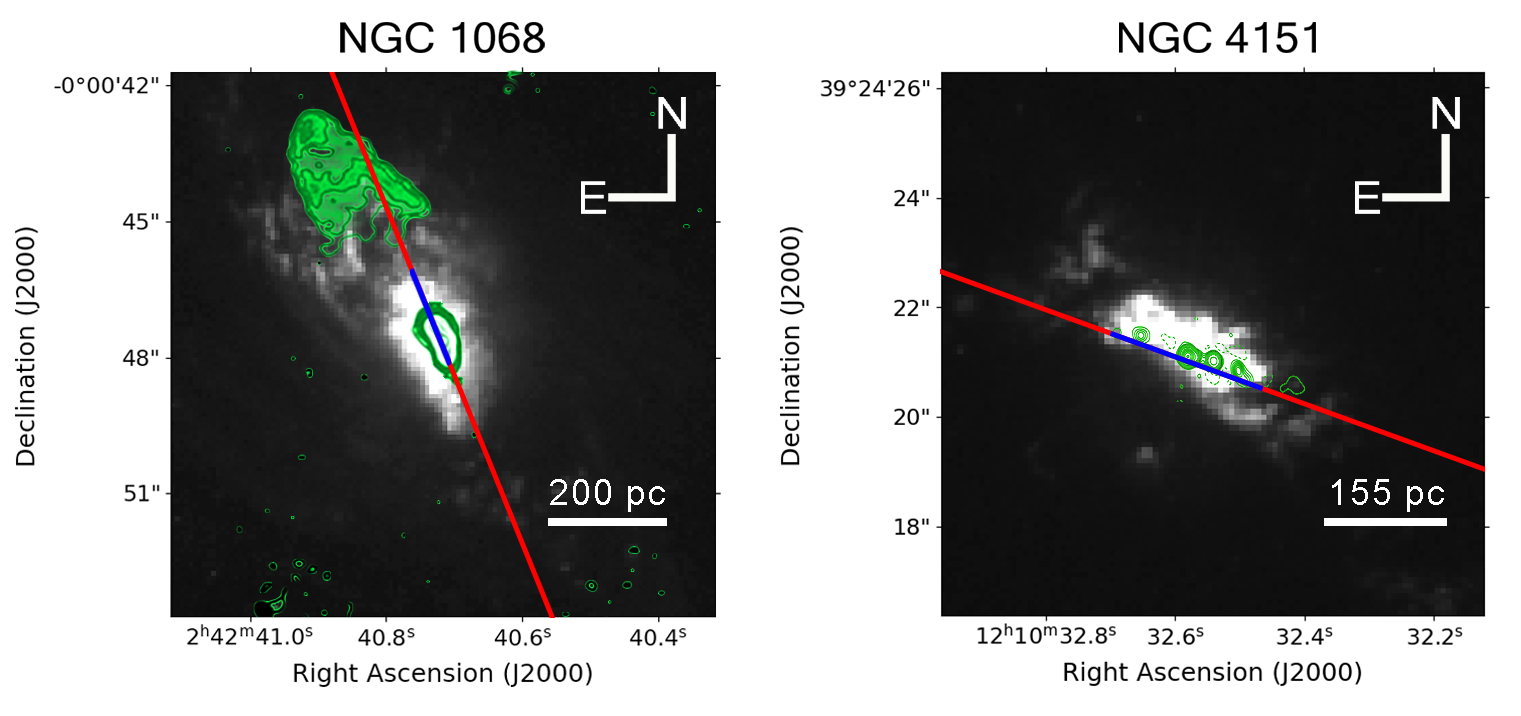
\includegraphics[width=1\linewidth]{figures/observations_and_data_reduction/seyferts_wfpc2.png}
    \caption[The slit positions of the archival HST/STIS observations plotted over archival {[}OIII{]} and radio-continuum imaging of NGC\;1068 and NGC\;4151.]{The slits of the archival STIS observations (red) shown plotted over archival HST/WFPC2 [OIII] emission-line images of the inner regions of NGC\;1068 and NGC\;4151, taken with the F502N filter (NGC\;1068: GTO:5754, PI Ford; NGC\;4151: GTO:5124; PI Ford). The spatial extents of the regions considered in this study (the extracted apertures: Section\;\ref{section: stis_seyferts: apertures}) along the slits are shown in blue. \textbf{Left:} The STIS slit shown over the [OIII] emission-line image of the near-nuclear regions of NGC\;1068; VLA 22\;GHz contours from \citet{Gallimore1996} are presented in green, showing the radio structure near the core and an extended lobe to the NE. \textbf{Right:} the STIS slit shown over the [OIII] emission-line image of the near-nuclear regions of NGC\;4151; the green contours are from high-resolution e-MERLIN 1.5\;GHz imaging presented by \citet{Williams2017}, and show a string of radio knots near the nucleus. I note that, while the narrow-band images are not continuum-subtracted, the brighter parts of the NLR emission are dominated by [OIII] emission in the filter bandpass, and so the images provide a good representation of the main NLR structures.}
    \label{fig: observations_and_data_reduction: stis_seyferts: observations: seyferts_wfpc2}
\end{figure*}

\subsection{Reduction of STIS data}
\label{section: stis_seyferts: observations_and_data_reduction data_reduction}

The first step in the data reduction was performed with the standard \mbox{\textsc{CALSTIS}} pipeline. For NGC\;1068, only a single exposure for each grating was available, while for NGC\;4151 I took the average of two exposures for each grating using \textsc{Python} scripts which made use of the \textsc{Numpy} \citep{Harris2020} and \mbox{\textsc{AstroPy}} \citep{AstropyCollaboration2013, AstropyCollaboration2018} modules. In order to ensure that the individual exposures for each grating were aligned, spatial slices were first extracted along the slit direction in a line-free region of the continuum covering the wavelength range 5480--5600\;{\AA} for the G430L grating and 6795--6890\;{\AA} for the G750L grating. The centroids of the spatial peaks --- determined with Gaussian-profile fits --- were consistent within 0.4\;pixels, confirming that each exposure was taken with the same telescope pointing within 0.02\;arcseconds. I also verified that the spectra taken with the G430L and G750L gratings for each object were aligned, using the same method of Gaussian-profile fits to the spatial flux profiles. Again, the spatial positions of the peak flux between gratings were consistent to within 0.4\;pixels, indicating that the observations with different gratings were closely spatially aligned.

Residual hot pixels and cosmic rays were removed from the spectra using the \textsc{CLEAN} command of the \textsc{STARLINK FIGARO} software package \citep{Currie2014}. Galactic-extinction correction was performed in the same manner as that done for IC\;5063 (Section\;\ref{section: xshooter_ic_5063: observations_and_data_reduction: data_reduction}) --- from the S98 and SF11 maps, the mean colour excesses in the directions of NGC\;1068 and NGC\;4151 were found to be \mbox{E(B-V)$_\mathrm{mean}=0.0289\pm0.0004$} and \mbox{E(B-V)$_\mathrm{mean}=0.0237\pm0.0011$}, respectively, and these values were used with the CCM89 $R_\mathrm{v}=3.1$ extinction law to correct for Galactic extinction.

\subsection{Aperture selection and extraction}
\label{section: stis_seyferts: apertures}

The reduced STIS long-slit spectra of NGC\;1068 and NGC\;4151 show disturbed kinematics (indicating outflows) and several bright emission-line knots in the central few hundred parsecs, as noted by previous studies \citep{Crenshaw2000a, Kraemer2000II, Das2005, Das2006, Meena2023}. Several apertures (integrated groupings of pixel rows) were extracted from the two-dimensional G430L and G750L spectra, following the methodology described in Section\;\ref{section: xshooter_ic_5063: observations_and_data_reduction: apertures}. Each aperture formed an integrated one-dimensional spectrum that corresponds to a certain spatial position along the slit, the locations of which were chosen to cover the locations of the bright emission knots seen in the two-dimensional spectra (Figure\;\ref{fig: stis_seyferts: apertures}). The widths of the apertures (6--15\;pixels; 0.3--0.8\;arcseconds) were set to contain sufficient signal in the emission lines that are used for diagnostics in this analysis, namely the fainter transauroral [OII]$\lambda\lambda$7319,7331 and [SII]$\lambda\lambda$4068,4076 doublets. The same apertures were extracted from the G430L and G750L spectra for each object, as it was previously determined that the spectra were closely spatially aligned. Flux errors were determined by adding the flux errors from individual pixel rows (which constitute a given aperture) in quadrature. As an example, part of the spectrum of Aperture 2 for NGC\;1068 is presented in Figure\;\ref{fig: stis_seyferts: ngc1068_g430l_ap2}. The chosen apertures extended to a maximum radial distance of 139\;pc for NGC\;1068, and 151\;pc in the case of NGC\;4151.

\begin{figure*}[!ht]
	\includegraphics[width=\linewidth, trim={-3.8cm 0 0 0}, clip]{figures/stis_seyferts/apertures.png}
	\caption[Long-slit spectra of NGC\;1068 and NGC\;4151, with the positions and sizes of extracted apertures overlaid.]{Apertures for NGC\;1068 (left) and NGC\;4151 (right), positioned over the [OIII]$\lambda\lambda$4959,5007 doublet in the two-dimensional STIS G430L spectra. The spectral direction is horizontal (left = bluewards; right = redwards) and the vertical direction is spatial along the slit (with the direction shown by the labelled arrows); velocity scale bars are shown in green, and spatial scale bars are shown to the right of each spectrum. The apertures are shown as regions bounded by dashed lines, and are labelled on the left of each image --- they were chosen to contain enough signal for the measurement of faint lines in distinct kinematic regions within the central few hundred parsecs of each galaxy.}
	\label{fig: stis_seyferts: apertures}
\end{figure*}

Aperture 3 for NGC\;1068 was placed over a bright emission knot that corresponds to a previously-detected radio source at the likely position of the galaxy's nucleus (see discussion in \citealt{Kraemer2000II}), while Aperture 4 for NGC\;4151 corresponds to the location along the slit that is closest to the nucleus. Note that the spectra for NGC\;4151 do not directly cover the nucleus due to the 0.1\;arcsecond slit offset to the south that was performed to avoid nuclear contamination. Unfortunately, the south-west part of the slit for NGC\;1068 (seen above Aperture 4 in Figure\;\ref{fig: stis_seyferts: apertures}) did not contain enough signal for the measurement of the faint [OII]$\lambda\lambda7319,7331$ transauroral doublet, even when integrated as a single aperture. Therefore, this region is omitted from any analysis. 

\begin{figure*}[!ht]
    \centering
    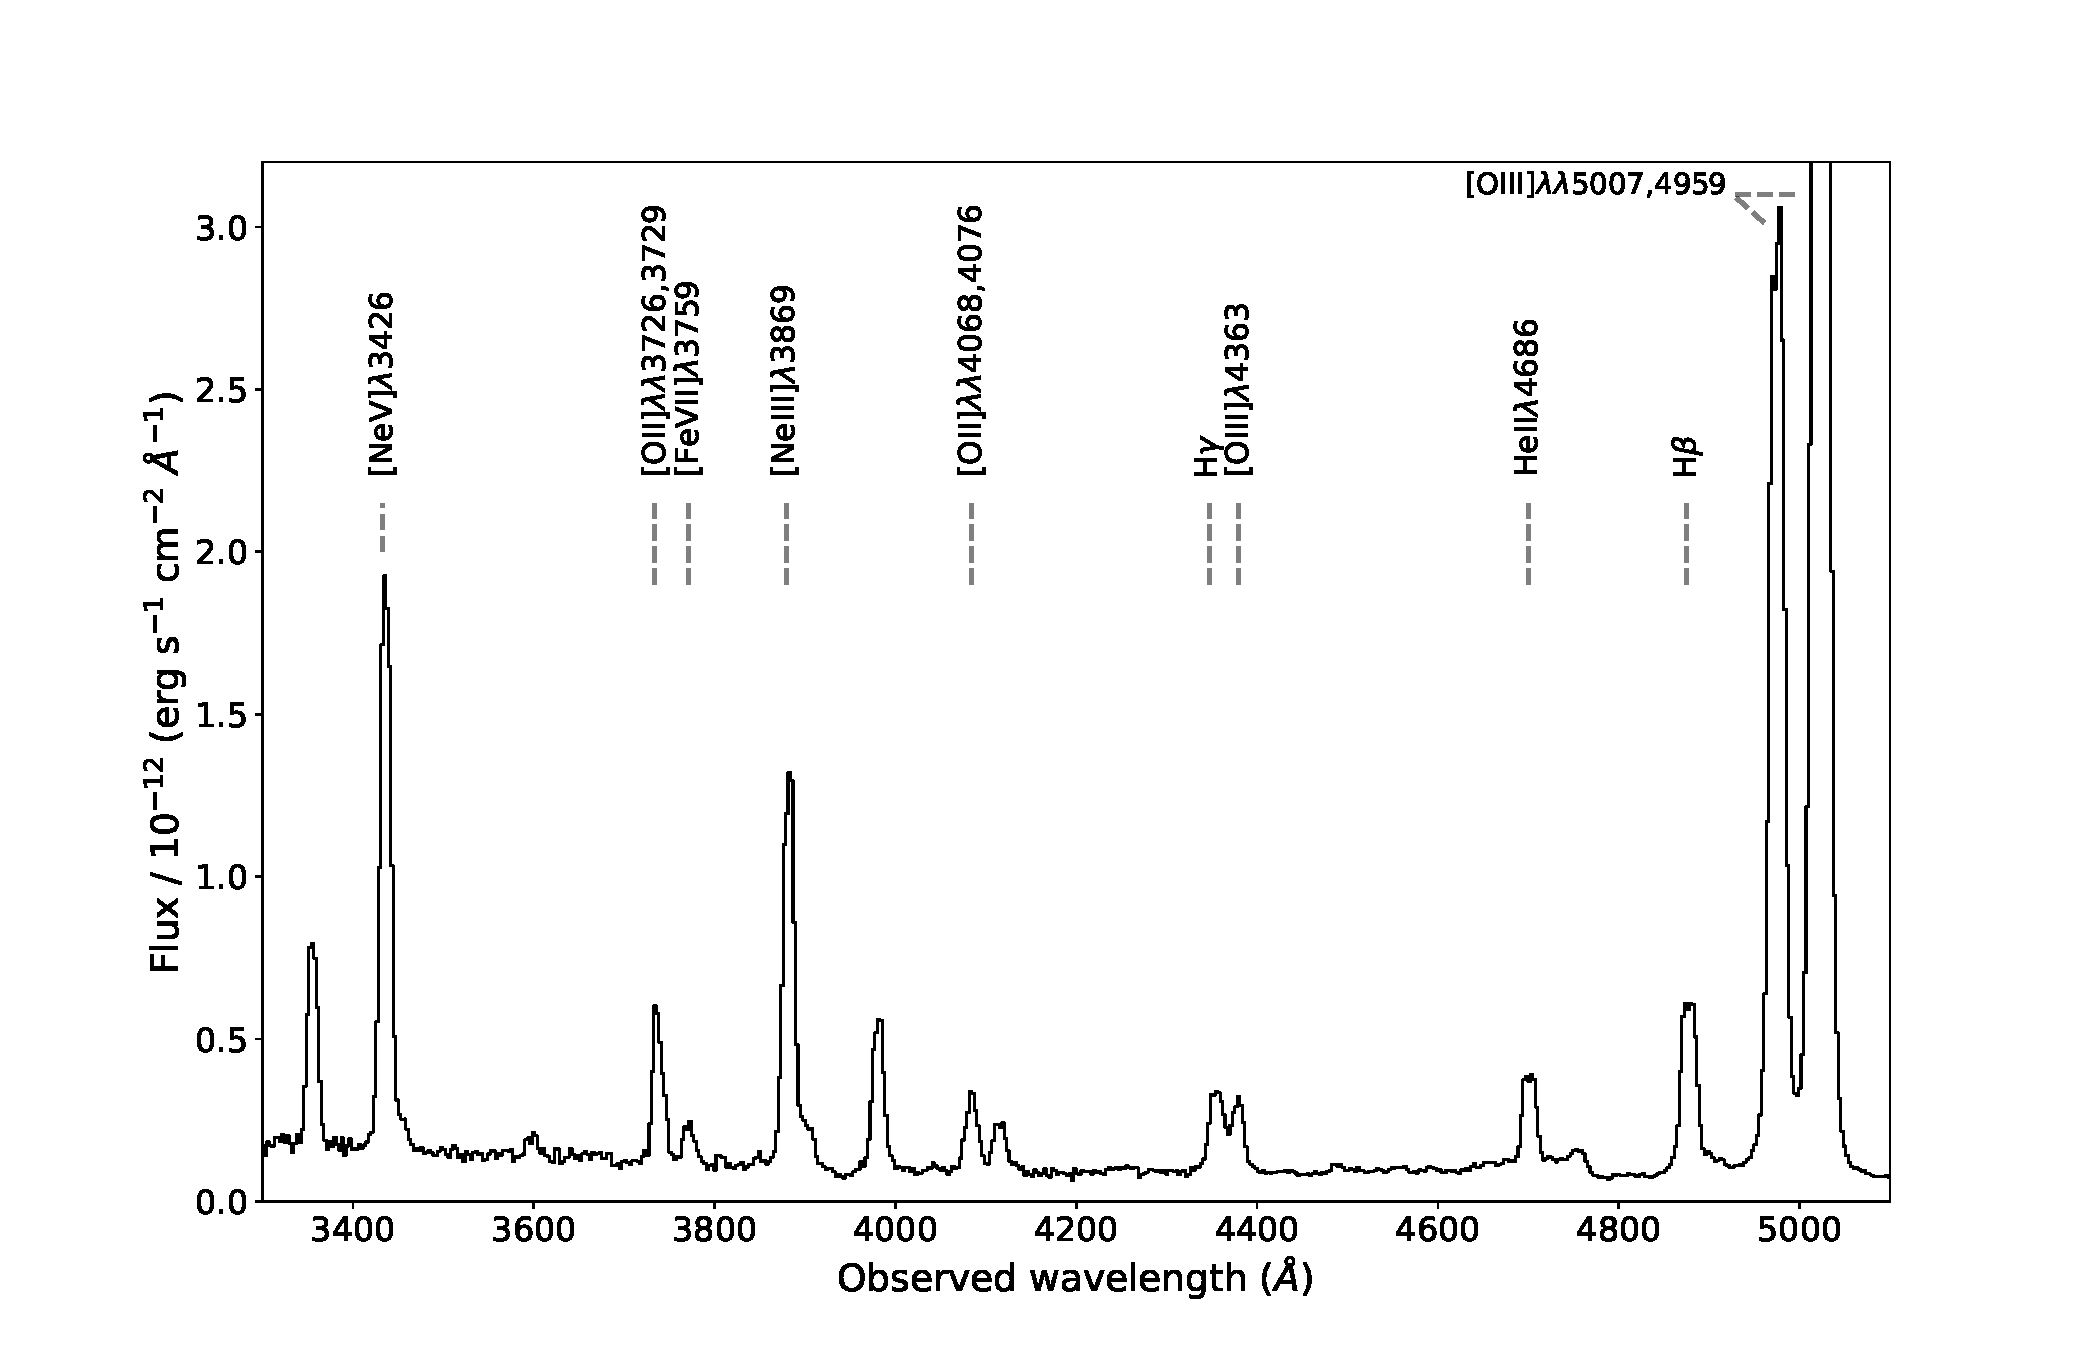
\includegraphics[width=\linewidth]{figures/stis_seyferts/ngc1068_g430l_ap2.pdf}
    \caption[HST/STIS G430L grating spectrum for Aperture 2 of NGC\;1068.]{The G430L grating spectrum for Aperture 2 of NGC\;1068 (Figure\;\ref{fig: stis_seyferts: apertures}). Key emission lines that are used in the analysis are labelled with dotted lines. Note that, for presentation reasons, the limit on the flux axis has been chosen so that fainter lines can be seen clearly; as a result, the peak of the [OIII]$\lambda$5007 line is not visible.}
    \label{fig: stis_seyferts: ngc1068_g430l_ap2}
\end{figure*}

Following aperture extraction, I ensured that the flux calibration was consistent between the two gratings for each aperture by overplotting the spectra in the region where the wavelength ranges of the gratings overlap (5275--5705\;{\AA}). It was found that all apertures for NGC\;1068 are closely matched in flux. However, for apertures 2 and 4 of NGC\;4151, the flux in the overlap region was \textgreater8\;per cent higher in the G430L grating than the G750L grating, potentially due to internal reflections within the instrument caused by the bright Type 1 nucleus (see \citealt{Nelson2000}). Therefore, these apertures are not used in further analysis. 

\subsection{The contribution of stellar continua to the spectra}
\label{section: stis_seyferts: stellar_continua}

The underlying stellar continua in NGC\;1068 and NGC\;4151 were not modelled and subtracted (as was done for IC\;5063: Section\;\ref{section: xshooter_ic_5063: observations_and_data_reduction: starlight}) for various reasons. First, the archival STIS G430L and G750L spectra did not have sufficient spectral resolution to clearly resolve absorption features that could be used to verify the robustness of the continuum fits. Second, there may be substantial contamination by direct and scattered AGN continuum \citep{Antonucci1985} and nebular continuum \citep{Tadhunter2016} that precludes accurate stellar-continuum modelling. Finally, the emission lines in the spectra have relatively-high equivalent widths, which fill in various stellar absorption features.

In order to verify whether stellar-continuum modelling was needed in this study, equivalent widths (EWs) for the H$\mathrm{\beta}$ recombination line were measured. Equivalent widths in the range \mbox{36\;\textless\;EW\;\textless\;148\;{\AA}} were found for the NGC\;1068 apertures and \mbox{30\;\textless\;EW\;\textless\;151\;{\AA}} for the NGC\;4151 apertures. The lowest measured emission-line equivalent width ($\mathrm{EW}=30$\;{\AA} for Aperture 3 in NGC\;4151) is a factor of three higher than that of the H$\mathrm{\beta}$ absorption feature as modelled for a $\sim$400\;Myr old stellar population (which gives the highest EWs in modelling by \citealt{GonzalezDelgado1999}). Thus, underlying stellar-absorption features may affect the H$\mathrm{\beta}$ luminosities measured in this work by a maximum factor of 1.3 (for a stellar $\mathrm{EW}=10$\;{\AA}). However, this is very much an upper limit since there is no clear Balmer break in the continua in any of the apertures, as would be expected for intermediate-age stellar populations that have strong Balmer absorption lines.

\subsection{Fits to key emission lines}
\label{section: stis_seyferts: oiii_models}

The NLR kinematics in NGC\;1068 and NGC\;4151 are complex, and have been previously modelled in detail as biconical outflows based on higher-resolution STIS spectra than those used here (\citealt{Das2006} and \citealt{Das2005} respectively; but see also \citealt{Crenshaw2000_N1068} and \citealt{Crenshaw2000_N4151}). In those studies, the [OIII]$\lambda\lambda$4959,5007 doublet line-profiles were fit with multiple Gaussian components for each pixel row of the two-dimensional spectra. Here, a similar procedure is performed for the extracted apertures by simultaneously fitting a first- or second-order polynomial to the continuum surrounding the [OIII]$\lambda\lambda$4959,5007 doublet, in addition to one or two Gaussian profiles to each of the lines within the doublet itself. The wavelength separation of the lines in the doublet, as well as the intensity ratio of the lines ($1:2.99$), were set to those defined by atomic physics \citep{Osterbrock2006}. Furthermore, the widths of a given Gaussian component were constrained to be the same for each line in the doublet. The resulting model parameters for each aperture are presented in Table \ref{tab: oiii_models}.

The difference between the mean wavelength of each Gaussian component and the rest [OIII] wavelength in the reference frame of the galaxy was calculated using redshifts\footnote{21\;cm redshifts from the NASA/IPAC Extragalactic Database (\url{https://ned.ipac.caltech.edu/}).} of $z=0.00381$ for NGC\;1068 and $z=0.003262$ for NGC\;4151. The intrinsic width of each component was also determined by subtracting the instrumental width of the STIS G430L grating in quadrature from the measured widths. According to the STIS manual, for a slit of width 0.1\;arcseconds, the instrumental broadening in the spectral direction is in the range \mbox{2\;\textless\;FWHM\;\textless\;3} pixels, corresponding to \mbox{5.5\;\textless\;FWHM\;\textless\;8.2\;{\AA}} for the G430L grating and \mbox{9.8\;\textless\;FWHM\;\textless\;14.8\;{\AA}} for the G750L grating. By fitting single Gaussian profiles to the [OIII]$\lambda\lambda$4959,5007 emission-line doublet at a radial distance of 4\;arcseconds from the nucleus of NGC\;4151 in the G430L spectra (where the lowest line widths are measured), a line width of FWHM$_\mathrm{inst}=6.0\pm0.4$\;{\AA} was measured; similarly, measuring the [SII]$\lambda$9531 line in the G750L spectra with this method resulted in a line width of FWHM$_\mathrm{inst}=12.3\pm2.4$\;{\AA}. Thus, instrumental widths of FWHM$_\mathrm{inst}=6.0$\;{\AA} (360\;km\;s$^{-1}$ at 5007\;{\AA}) and FWHM$_\mathrm{inst}=12.3$\;{\AA} (560\;km\;s$^{-1}$ at 6575\;{\AA}) are adopted here for the G430L and G750L gratings, respectively.

In subsequent analysis, only \textit{total} line fluxes --- including all Gaussian components used --- are considered, rather than fluxes from individual components (i.e. potentially representing outflowing and quiescent gas). This was done because the low spectral resolutions of the G430L and G750L gratings made it challenging to separate different kinematic components in cases where lines are heavily blended. Nonetheless, in order to improve the accuracy of the fits to the weaker emission lines and blends in the spectra, the kinematics (velocity shifts and widths) derived from fits to the [OIII] doublet in each aperture were used to constrain the fits to the other key diagnostic lines, such as H$\mathrm{\beta}$, H$\mathrm{\gamma}$, [OIII]$\lambda$4363, [OII]$\lambda$3726,3729, [OII]$\lambda\lambda$7319,7331, [SII]$\lambda\lambda$4068,4076, [SII]$\lambda\lambda$6717,6731, [ArIV]$\lambda\lambda$4711,4740 and HeII$\lambda$4686. It was found that this procedure produced acceptable fits to these lines, including the transauroral [SII]$\lambda\lambda$4068,4076 and [OII]$\lambda\lambda$7319,7331 doublets. However, for closely spaced doublets such as [OII]$\lambda$3726,3729, the low spectral resolution meant that individual lines were not resolved, and so the \textit{total} doublet profile was modelled as a single emission line during the fitting process.

\begin{table*}
    \def\arraystretch{1.2}
    \centering
    \begin{tabular}{lcccccc}
    \multirow{2}{*}{Aperture} & Distance & Distance  & $v_\mathrm{c, a}$ & FWHM$_\mathrm{c, a}$ & $v_\mathrm{c, b}$ & FWHM$_\mathrm{c, b}$ \\ 
        & (arcseconds) & (pc) & (km\;s$^{-1}$) & (km\;s$^{-1}$) & (km\;s$^{-1}$) & (km\;s$^{-1}$) \\
    \multicolumn{7}{c}{\vspace{-0.4cm}} \\
    \multicolumn{7}{c}{NGC 1068} \\ \hline
    1 & $-1.45$ & $-97$ & $-828\pm$4 & 572$\pm$25 & 295$\pm$40 & 1078$\pm$96 \\
    2 & $-0.74$ & $-50$ & $-184\pm$7 & 1017$\pm$31 & --- & --- \\
    3 & $-0.23$ & $-15$ & $-306\pm$3 & 662$\pm$26 & $-5\pm$20 & 1770$\pm$43 \\
    4 & $0.10$ & $7$ & $95\pm$3 & 367$\pm$26 & 235$\pm$8 & 1684$\pm$34 \\
    \multicolumn{7}{c}{\vspace{-0.4cm}} \\
    \multicolumn{7}{c}{NGC 4151} \\ \hline
    1 & $-1.58$ & $-123$ & $-172\pm$2 & 420$\pm$25 & $-263\pm$29 & 1261$\pm$102 \\
    3 & $-0.38$ & $-30$ & $-392\pm$6 & 0$\pm28$\;$^a$ & $-356\pm$3 & 1065$\pm$26 \\
    5 & 0.48 & $37$ & $34\pm$1 & 234$\pm$24 & 121$\pm$11 & 1013$\pm$44 \\
    6 & 1.02 & $80$ & $40\pm$1 & 307$\pm$25 & 126$\pm$8 & 768$\pm$35 \\
    \end{tabular} \\
    \vspace{12pt}
    $^a$ The measured width of the \textit{component} is consistent with the instrumental width, and hence unresolved. \\
    \caption[{[}OIII{]} model parameters and aperture distances for each of the apertures for NGC\;1068 and NGC\;4151.]{[OIII] model parameters (galaxy rest-frame component velocity shift: $v_\mathrm{c}$; instrumentally-corrected component velocity width: FWHM$_{c}$) and distances from the nucleus (in arcseconds and pc) for each of the apertures for NGC\;1068 and NGC\;4151. In apertures where there are multiple Gaussian components for the [OIII] models, the kinematic parameters for the two components are labelled with the subscripts `a' and `b'.}
    \label{tab: oiii_models}
\end{table*}

\section{Analysis of the STIS spectra}
\label{section: stis_seyferts: analysis}

\subsection{Transauroral-line diagnostics}
\label{section: stis_seyferts: tr_diagnostics}

In order to provide estimates of the electron densities of the warm-ionised gas in NGC\;1068 and NGC\;4151, I made use of the transauroral-line-ratio technique (first described by \citealt{Holt2011}) that was verified and used in Chapter \ref{chapter: xshooter_ic5063}, for two key reasons. First, these lines have sufficiently-high critical densities (Appendix \ref{appendix: properties_of_warm_ionised_diagnostic_lines}) to be sensitive to the electron density values that have previously been determined for these objects ($10^{3.0}$\;\textless\;$n_e$\;\textless\;$10^{7.2}$\;cm$^{-3}$). Second, because the transauroral-line method uses the ratios of the \textit{total} line fluxes of widely-separated emission-line doublets (unlike the commonly-used [OII](3726/3729) and [SII](6717/6731) ratios), this method is less susceptible to uncertainties from fit degeneracy resulting from the larger velocity widths (as is often the case for outflowing gas) and low spectral resolutions (as for the G430L and G750L STIS gratings) that lead to the blending of line profiles within the doublets. 

\newpage
The [OIII] models were fit to the transauroral lines to measure line fluxes, which were then used to calculate the TR ratios
\begin{align*}
TR([OII]) = F(3726 + 3729) / F(7319 + 7331), \\
TR([SII]) = F(4068 + 4076) / F(6717 + 6731).
\end{align*} 
As in Chapter \ref{chapter: xshooter_ic5063}, the \textsc{CLOUDY} code (version C17.02: \citealt{Ferland2017}) was used to generate plane-parallel, single-slab, radiation-bounded models of solar-composition gas with no dust depletion, photoionised by a central source. The ionising continuum of this source followed a power-law of shape $F_v \propto v^{-\alpha}$ between 10\;{\textmu}m and 50\;keV, with a spectral index of $\alpha=1.5$. I note, however, that the TR ratios are relatively insensitive to the shape of the ionising continuum (see Appendix B in \citealt{Santoro2020}). The ionisation parameter was set to log\;$U=-3$ (the highest value that reproduced the measured TR ratios), and the electron density of the modelled gas was varied in 0.01\;dex steps between \mbox{2.00\;\textless\;log$_{10}(n_e$ [cm$^{-3}$])\;\textless\;5.00}. The modelled TR ratios produced for each electron density value were then reddened with the $R_\mathrm{v}=3.1$ CCM89 law, producing a grid of values that could be compared to the measured ratios in order to provide simultaneous determinations of electron density and reddening. The resulting TR grid is shown in Figure\;\ref{fig: stis_seyferts: tr_ddd}, and the derived values are given in Table {\ref{tab: stis_seyferts: ne_ebv_te}}.

\begin{table*}
    \def\arraystretch{1.4}
    \centering
    \begin{tabular}{lccc}
    Aperture & log$_{10}(n_e$[cm$^{-3}$]) & E(B-V)$_\mathrm{TR}$ & $T_e$ (K) \\ 
    \multicolumn{4}{c}{\vspace{-0.4cm}} \\
    \multicolumn{4}{c}{NGC\;1068} \\ 
    \hline
    1 & 4.06$^{+0.05}_{-0.06}$ & 0.16$^{+0.04}_{-0.05}$ & 14300$^{+2100}_{-1300}$ \\
    2 & 4.65$^{+0.05}_{-0.04}$ & 0.05$^{+0.04}_{-0.05}$ & 14400$^{+1500}_{-1100}$ \\
    3 & 4.74$^{+0.05}_{-0.05}$ & 0.16$^{+0.05}_{-0.04}$ & 16100$^{+1400}_{-1000}$ \\
    4 & 4.45$^{+0.09}_{-0.09}$ & 0.17$^{+0.08}_{-0.08}$ & 16000$^{+1600}_{-1100}$ \\
    \multicolumn{4}{c}{\vspace{-0.4cm}} \\
    \multicolumn{4}{c}{NGC\;4151} \\ 
    \hline
    1 & 3.68$^{+0.08}_{-0.10}$ & 0.11$^{+0.05}_{-0.07}$ & 16300$^{+3400}_{-1800}$ \\
    3 & 4.04$^{+0.07}_{-0.15}$ & 0.13$^{+0.05}_{-0.06}$ & 21000$^{+3300}_{-2100}$ \\
    5 & 3.94$^{+0.10}_{-0.10}$ & 0.15$^{+0.08}_{-0.08}$ & 17300$^{+5200}_{-2400}$ \\
    6 & 3.75$^{+0.8}_{-0.10}$  & 0.23$^{+0.07}_{-0.07}$ & 15200$^{+3400}_{-1800}$ \\
    \end{tabular}
    \caption[Electron densities, reddening values, and electron temperatures for NGC\;1068 and NGC\;4151.]{Electron densities, reddening values and electron temperatures for the NGC\;1068 and NGC\;4151 apertures. The densities and reddenings were determined simultaneously using the transauroral-line technique (Section\;\ref{section: stis_seyferts: tr_diagnostics}; Figure\;\ref{fig: stis_seyferts: tr_ddd}), and the temperatures were determined using the [OIII](5007+4959)/4363 ratio (Section\;\ref{section: stis_seyferts: electron_temperatures}).}
    \label{tab: stis_seyferts: ne_ebv_te}
\end{table*}

The electron densities measured in this way for NGC\;1068 have values in the range \mbox{4.00\;\textless\;log$_{10}(n_e$\;[cm$^{-3}$])\;\textless\;4.75}, while those for NGC\;4151 are approximately an order of magnitude lower (\mbox{3.60\;\textless\;log$_{10}(n_e$\;[cm$^{-3}$])\;\textless\;4.10}). This is the first time that densities above $n_e=10^{3.5}$\;cm$^{-3}$ have been found using the transauroral lines with \textit{spatially-resolved} observations; these values agree with similarly high electron densities derived using this technique for non-spatially resolved observations of other AGN (e.g. \citealt{Holt2011, Rose2018, Santoro2018, Spence2018, Davies2020, Speranza2022}). Importantly, the densities found here are above the upper sensitivity limit of the traditional [OII](3726/3729) and [SII](6717/6731) line ratios (Appendix \ref{appendix: properties_of_warm_ionised_diagnostic_lines}), and since broad (outflowing) and narrow (quiescent; non-outflowing) components are not separated, are likely to be underestimates for the outflowing gas (which is expected to be denser than the quiescent gas: e.g. \citealt{VillarMartin1999}; Chapter \ref{chapter: xshooter_ic5063}). The reddening values that are measured are relatively modest, and in the range \mbox{0.05\;\textless\;E(B-V)$_\mathrm{TR}$\;\textless\;0.25} for both objects --- these values were used to deredden the spectra for all further analysis.

\begin{figure}[!t]
    \centering
    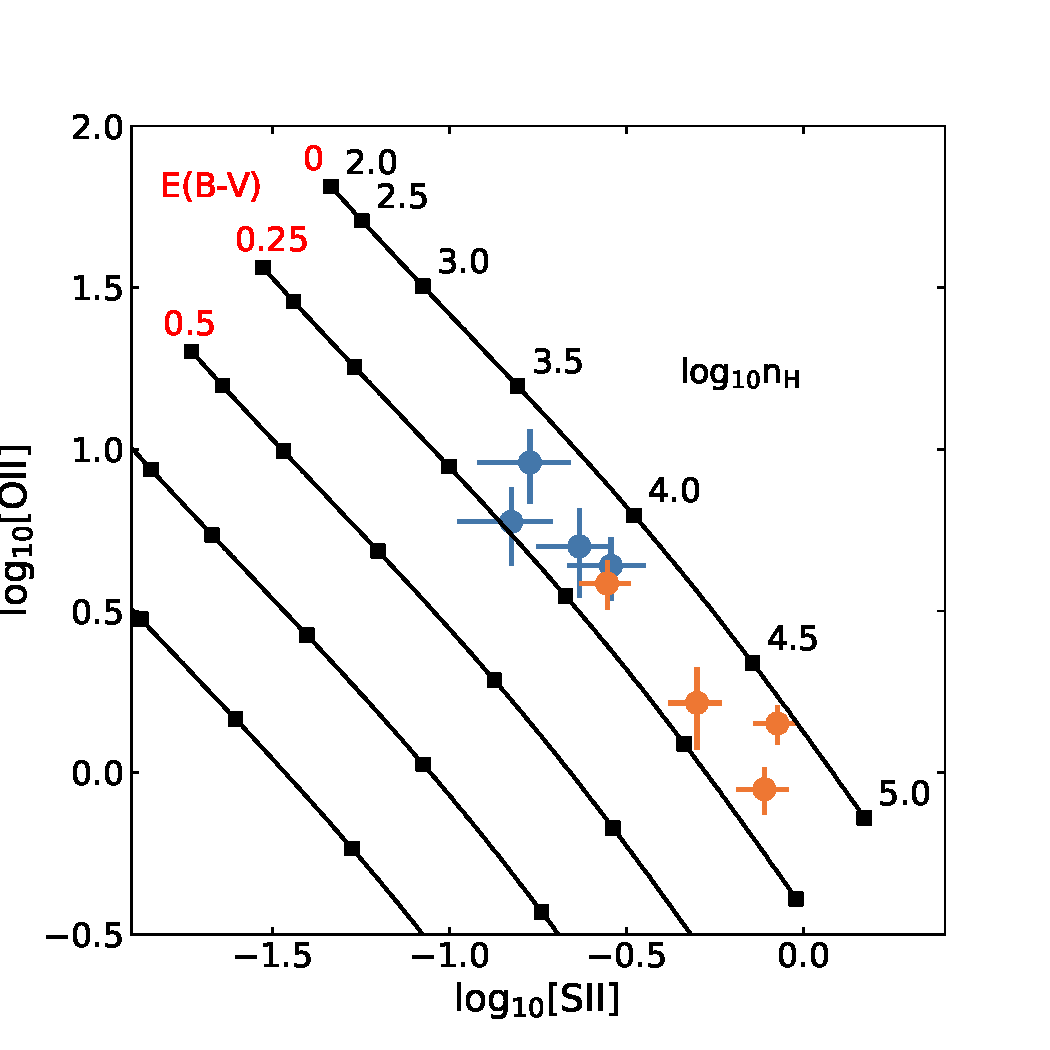
\includegraphics[width=0.8\linewidth]{figures/stis_seyferts/tr_ddd_seyferts.pdf}
    \caption[Transauroral {[}OII{]} and {[}SII{]} line ratio diagram for NGC\;1068 and NGC\;4151, showing both measured values and those predicted from photoionisation modelling.]{Grid of modelled transauroral (TR) [SII] and [OII] line ratios for radiation-bounded gas at different electron densities and reddenings (black joined squares; as modelled with the \textsc{Cloudy} code and the CCM89 extinction curve), and measured line ratios for the NGC\;1068 (orange circles) and NGC\;4151 (blue circles) apertures.}
    \label{fig: stis_seyferts: tr_ddd}
\end{figure}

\subsection{Ionisation states and mechanisms of the warm-ionised gas}
\label{section: stis_seyferts: mechanisms}

The relatively-low-ionisation transauroral lines must be emitted by radiation-bounded clouds --- therefore, it is uncertain how well densities derived from the transauroral ratios would represent the densities of clouds or cloud complexes that have been shock-ionised or have significant matter-bounded components. Furthermore, the model used in the transauroral-ratio method assumes radiation-bounded AGN-photoionised clouds, with no contribution from a matter-bounded component or shock-ionisation. Similarly, the multi-component ionisation modelling by \citet{Revalski2021} --- which has previously been applied to NGC\;1068 and NGC\;4151 --- uses AGN-photoionisation models. Therefore, it is important to investigate the ionisation mechanisms for the gas detected in the STIS slits, which potentially can also give information regarding the outflow acceleration mechanism(s) present.

\subsubsection{Electron temperatures}
\label{section: stis_seyferts: electron_temperatures}

Electron temperatures of the warm ionised phase are expected to be higher for shocked gas than AGN-photoionised gas (e.g. \citealt{Fosbury1978, VillarMartin1999}). Therefore, to provide a first indication of the ionisation mechanisms of the warm-ionised gas observed in the apertures, electron temperatures were measured using the (dereddened) [OIII](5007+4959)/4363 emission-line ratio and the \textsc{PyNeb Python} module \citep{Luridiana2015}, taking the electron densities for the apertures to be those derived using the transauroral-line technique for both objects (3.75\;\textless\;log$_{10}(n_e$\;[cm$^{-3}$])\;\textless\;4.75: see Table\;\ref{tab: stis_seyferts: ne_ebv_te} and Section\;\ref{section: stis_seyferts: tr_diagnostics}). Electron temperatures measured in this way are presented in Table\;\ref{tab: stis_seyferts: ne_ebv_te} --- values in the range $14,300$\;\textless\;$T_e$\;\textless\;$21,000$\;K are found for every aperture in both objects, with the highest temperatures (up to $T_e=21,000$\;K) being found in the central apertures of NGC\;4151. These high electron temperatures may not be fully explainable as being due to AGN-photoionisation of radiation-bounded gas (\citealt{Fosbury1978, Binette1996, VillarMartin1999}; Chapter \ref{chapter: xshooter_ic5063}).

\subsubsection{Shock-ionisation vs matter-bounded AGN-photoionisation}
\label{section: stis_seyferts: shock_vs_agn}

In order to investigate the cause of the high electron temperatures further, the [OIII](5007/4363) vs HeII/H$\mathrm{\beta}$ diagnostic diagram (developed by \citealt{VillarMartin1999}) was produced for the apertures for NGC\;1068 and NGC\;4151 --- this is shown in Figure\;\ref{fig: stis_seyferts: oiii_heii_hbeta_stis}. The radiation-bounded photoionisation models shown here are the same as those used for the TR ratio grid in Section\;\ref{section: stis_seyferts: tr_diagnostics} (Figure\;\ref{fig: stis_seyferts: tr_ddd}), albeit for an electron density of $n_e=10^{4}$\;cm$^{-3}$, varying ionisation parameters (between $-3.5$\;\textless\;log$_{10}U$\;\textless\;$-2.0$), and two values of spectral index ($\alpha=1.0$, 1.5)\footnote{The effect of varying the photoionisation model parameters on the [OIII](5007/4363) vs HeII/H$\mathrm{\beta}$ diagnostic diagram is investigated in Appendix \ref{appendix: heii_hb_oiii_photoionisation_modelling}.}. The pure-shock and precursor (pre-shock) models are taken from the \textsc{MAPPINGS III} library presented by \citet{Allen2008}, with varying shock velocities in the range 100\;\textless\;$v_\mathrm{shock}$\;\textless\;1000\;km\;s$^{-1}$ and magnetic parameters of \mbox{$B/\sqrt{n}$ = 2,4\;$\mu$G\;cm$^{3/2}$} for a solar-composition pre-shock gas with a density of \mbox{$n$ = 10$^{2}$\;cm$^{-3}$}. The magnetic parameters were chosen to cover a reasonable range of values expected in the ISM \citep{Dopita1995}, in addition to being close to the magnetic parameters near equipartition (\mbox{$B/\sqrt{n}\sim3.23\;\mu$G\;cm$^{3/2}$}: \citealt{Allen2008}). Note that, as in Chapter \ref{chapter: xshooter_ic5063}, the standard `BPT' diagrams \citep{Baldwin1981} are not used here to investigate the ionisation of the gas because the regions of photo- and shock-ionisation in those diagrams overlap considerably (see Section\;\ref{section: introduction: outflows: accleration_mechanisms: ionisation_and_excitation_mechanisms}, Figure\;\ref{fig: introduction: outflows: acceleration_mechanisms: bpt_diagram_photo_shock_ionisation}). Furthermore, some of the lines involved in those diagrams (such as H$\mathrm{\alpha}$ and [NII]$\lambda\lambda$6548,6583) are strongly blended in the apertures considered here due to the outflow kinematics and the relatively-low spectral resolution, and therefore are affected by major fit degeneracies.

In Figure\;\ref{fig: stis_seyferts: oiii_heii_hbeta_stis}, the [OIII](5007/4363) and HeII/H$\mathrm{\beta}$ line ratios are also plotted as functions of A$_\mathrm{M/I}$: the ratio of the solid angles subtended by matter-bounded clouds and radiation-bounded clouds, from modelling by \citet{Binette1996}. This ratio allows estimations of the relative contribution of matter-bounded clouds and radiation-bounded clouds in the apertures. The modelling by \citet{Binette1996} assumes solar-metallicity gas, with an ionising-source spectral index of $\alpha=-1.3$, an ionisation parameter of log\;$U=-1.4$, and a density of $n_\mathrm{MB}=50$\;cm$^{-3}$. In this model, the radiation-bounded clouds are ionised by UV photons which have passed through the matter-bounded component, thus the shape of the ionising spectrum reaching the radiation-bounded clouds has changed relative to that from the source --- the parameters of the radiation-bounded clouds are determined using the resulting ionising spectrum and by assuming that the clouds have fixed pressures.

Due to line-blending effects and the continuum underlying the H$\mathrm{\beta}$, [HeII]$\lambda$4686, and [OIII]$\lambda$4363 lines being more complex than that which underlies the [OIII]$\lambda\lambda$4959,5007 doublet and transauroral lines, an MCMC (Markov Chain Monte Carlo) fitting routine was used to fit the lines involved in the HeII$\lambda$4686/H$\mathrm{\beta}$ and [OIII](5007/4363) ratios in each aperture for both objects --- this was done to ensure that line-flux uncertainties were not significantly overestimated due to the blending of spectral lines and the continuum. The results of the Gaussian fits described in Section\;\ref{section: stis_seyferts: oiii_models} (determined using least-squares optimisation) to these lines were used as initial starting points for the MCMC routine, which fit the same models (namely one or two Gaussian components and a low-order polynomial) to the spectra --- taking into account the flux uncertainty of the HST data --- with priors chosen to ensure that the resulting models were physical (i.e. the line fluxes, mean wavelengths, and line widths must have been positive). For each fit, 500 walkers were initialised in a Gaussian distribution around the starting parameters, and 5000 iterations (including a 1000 iteration `burn-in' phase) were used. The MCMC fits themselves were run using the \textsc{emcee} \textsc{Python} module \citep{FormanMackey2013}.

\begin{figure}[!p]
    \centering
    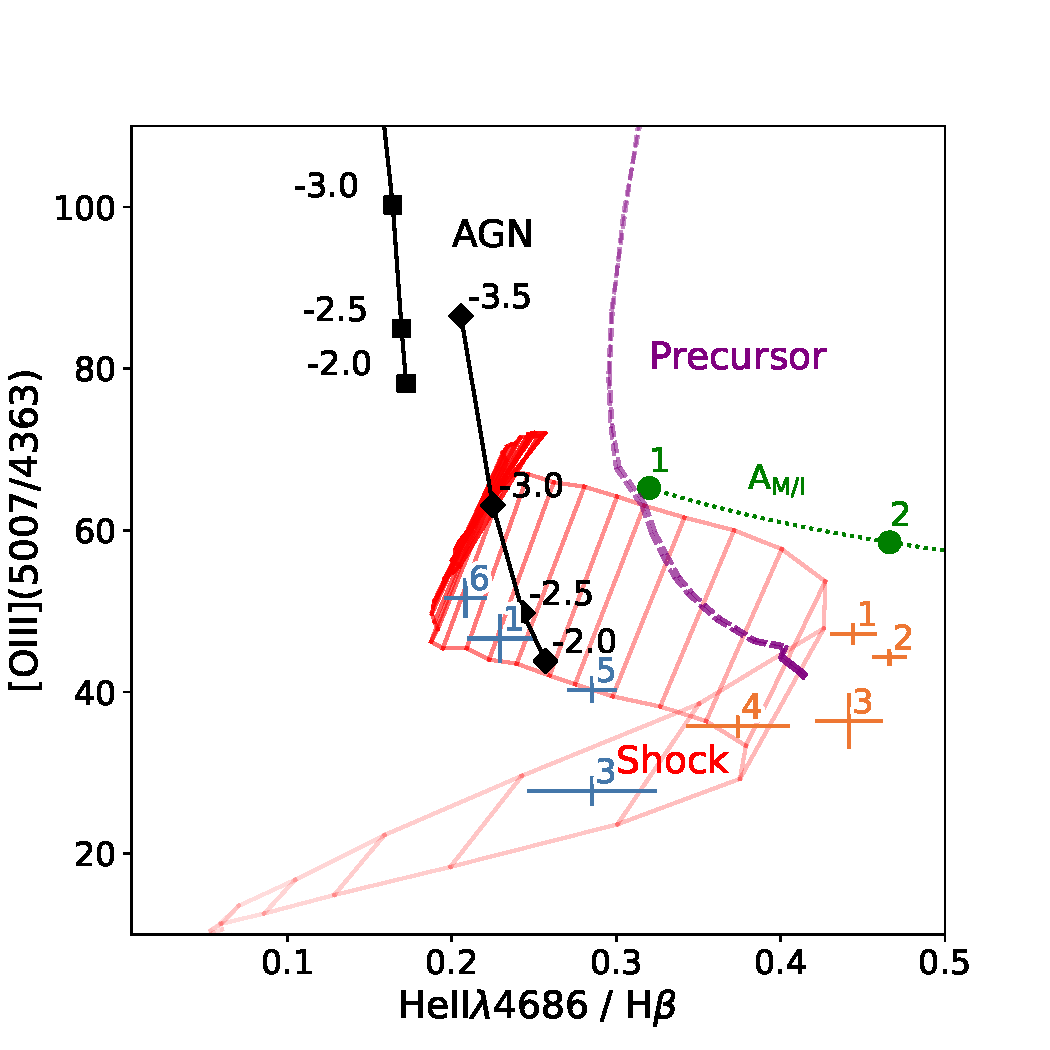
\includegraphics[width=0.8\linewidth]{figures/stis_seyferts/oiii_heii_hb_stis.pdf}
    \caption[HeII$\lambda$4686/H$\mathrm{\beta}$ vs {[}OIII{]}5007/{[}OIII{]}$\lambda$4363 diagnostic diagram for the warm-ionised gas in NGC\;1068 and NGC\;4151, including modelled values for (radiation-bounded and matter-bounded) photo- and shock-ionised gas.]{[OIII](5007/4363) vs HeII/H$\mathrm{\beta}$ diagnostic diagram \citep{VillarMartin1999}, used to distinguish between radiation-bounded AGN-photoionisation, matter-bounded AGN-photoionisation, and shock-ionisation. The black markers show the predicted line ratios from radiation-bounded \textsc{Cloudy} modelling (see Section\;\ref{section: stis_seyferts: tr_diagnostics}) for solar-composition gas with a density of \mbox{$n_e=10^{4}$\;cm$^{-3}$} and varying ionisation parameters (log\;$U$; labelled) and spectral indices (squares: $\alpha=1.5$; diamonds: $\alpha=1.0$). The solid red grid shows the line ratios predicted from shock modelling \citep{Allen2008} for solar-composition gas with a pre-shock density of \mbox{$n$ = 10$^{2}$\;cm$^{-3}$} and magnetic parameters of \mbox{$B/\sqrt{n}=2,4$\;$\mu$G\;cm$^{3/2}$}, with lighter regions on the plot corresponding to lower shock velocities. The purple dashed lines show the predicted emission from the precursor gas, which has not yet passed through (but is photoionised by) the shock, and the dotted green line shows the line ratios expected for different ratios of matter-bounded and radiation-bounded clouds (A$_\mathrm{M/I}$, labelled and marked with green circles) from photoionisation modelling by \citet{Binette1996}. Observed line ratios for each aperture are shown in orange for NGC\;1068 and blue for NGC\;4151, with the aperture number annotated.}
    \label{fig: stis_seyferts: oiii_heii_hbeta_stis}
\end{figure}

From Figure\;\ref{fig: stis_seyferts: oiii_heii_hbeta_stis}, there is clear evidence for significant matter-bounded emission in apertures 1, 2, and 3 in NGC\;1068, implied by high electron temperatures and HeII/H$\mathrm{\beta}$\;\textgreater\;0.4 (similar ratio values were also measured by \citealt{Kraemer2000III}); the approximate ratio of matter-bounded to radiation-bounded clouds is A$_\mathrm{M/I}\sim2$. The difference between the [OIII](5007/4363) ratios measured in the NGC\;1068 apertures and those predicted from the \citet{Binette1996} modelling can be explained as the models only representing one combination of parameters: it is possible for matter-bounded clouds with different parameters to have similar [OIII](5007/4363) ratios to those found for NGC\;1068. Specifically, this ratio would be smaller for higher electron densities than the low density assumed by \citet{Binette1996}. Moreover, the presence of matter-bounded emission in these apertures is supported by the strength of high-ionisation coronal emission lines (E$_\mathrm{ion}$\;\textgreater\;100\;eV), such as [NeV]$\lambda$3426, [FeVII]$\lambda$3759, and [FeVII]$\lambda$6087, relative to lower-ionisation lines (such as [OIII]) in the STIS spectra. These and other high-ionisation lines were previously identified in the same dataset by \citet{Kraemer2000II}. For Aperture 4 of NGC\;1068 (centred slightly above the nucleus: Figure\;\ref{fig: stis_seyferts: apertures}), the  HeII/H$\mathrm{\beta}$ ratios are consistent with both matter-bounded AGN-photoionisation and shock-ionisation. 

\begin{figure}[!t]
\centering
    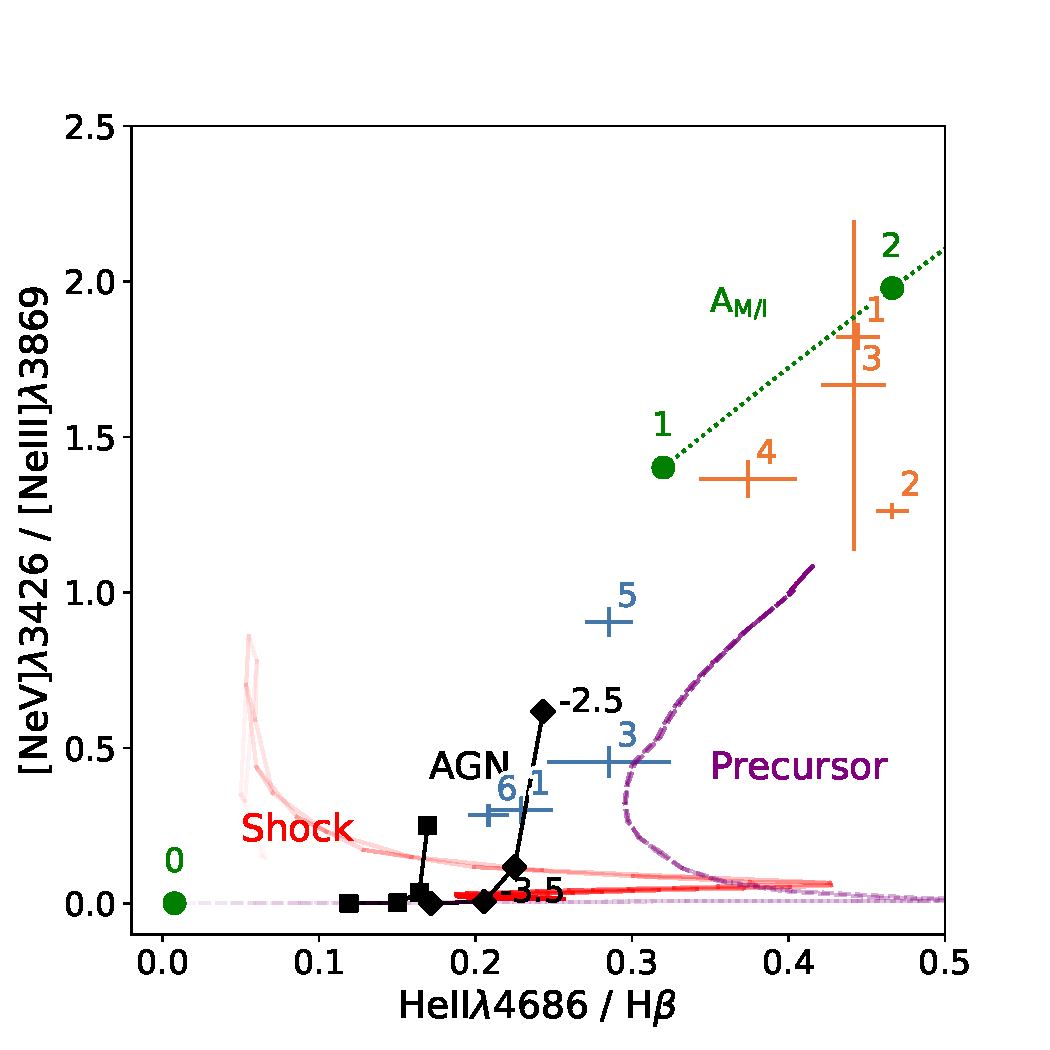
\includegraphics[width=0.8\linewidth]{figures/stis_seyferts/heii_nev_neii.pdf}
    \caption[{[}NeV{]}3426/{[}NeIII{]}3869 vs HeII/H$\mathrm{\beta}$ diagnostic diagram for the warm-ionised gas in NGC\;1068 and NGC\;4151, including modelled values for (radiation-bounded and matter-bounded) photo- and shock-ionised gas.]{[NeV]3426/[NeIII]3869 vs HeII/H$\mathrm{\beta}$ diagnostic diagram --- both ratios are sensitive to the presence of significant matter-bounded components. The line and marker scheme is the same as Figure\;\ref{fig: stis_seyferts: oiii_heii_hbeta_stis}. The line ratios measured in the NGC\;1068 apertures are located in the matter-bounded photoionisation region of the diagram (corresponding to \mbox{1\;\textless\;A$_\mathrm{M/I}$\;\textless\;2}; consistent with Figure\;\ref{fig: stis_seyferts:nev_neiii_heii_hbeta_stis}) whereas the NGC\;4151 line ratios fall in the shock/precursor/radiation-bounded AGN-photoionisation region.}
    \label{fig: stis_seyferts:nev_neiii_heii_hbeta_stis}
\end{figure}

To further probe the ionisation mechanism of the gas, the [NeV]$\lambda$3426/[NeIII]$\lambda$3869 ratio --- which is sensitive to higher-ionisation gas --- was also measured using the same MCMC fitting routine described earlier. A diagnostic diagram of [NeV]$\lambda$3426/[NeIII]$\lambda$3869 vs HeII/H$\mathrm{\beta}$ --- presented in Figure\;\ref{fig: stis_seyferts:nev_neiii_heii_hbeta_stis} --- was produced using the same radiation-bounded-photoionisation, matter-bounded-photoionisation, and shock-ionisation models as used for the [OIII](5007/4363) and HeII/H$\mathrm{\beta}$ diagram. It is found that the values for all of the NGC\;1068 apertures are consistent with matter-bounded AGN-photoionisation with  1\;\textless\;A$_\mathrm{M/I}$\;\textless\;2, further indicating that the gas in these apertures is matter-bounded and AGN-photoionised, including Aperture 4.

With the exception of Aperture 3, the [OIII](5007/4363) vs HeII/H$\mathrm{\beta}$ ratios measured in the NGC\;4151 apertures (Figure\;\ref{fig: stis_seyferts: oiii_heii_hbeta_stis}), are consistent with both shock-ionisation and radiation-bounded AGN-photoionisation (assuming a relatively flat spectral index of $\alpha=1.0$ and log\;$U\sim-2.0$). However, from the [NeV]$\lambda$3426/[NeIII]$\lambda$3869 vs HeII/H$\mathrm{\beta}$ diagram (Figure\;\ref{fig: stis_seyferts:nev_neiii_heii_hbeta_stis}), it can be seen that the measured ratios for NGC\;4151 are not consistent with pure shock-ionisation alone: if the gas is shock-ionised, then a contribution from the precursor component is required. Alternatively, the gas in these apertures may have pure radiation-bounded AGN-photoionisation, however, I highlight that this requires a relatively flat spectral index ($\alpha=1.0$), and/or higher ionisation parameters ($-3.0$\;\textless\;log\;$U$\;\textless\;$-2.0$) and densities ($n_e$\;\textgreater\;$10^5$\;cm$^{-3}$) than can explain the measured transauroral-line ratios (Section\;\ref{section: stis_seyferts: tr_diagnostics}). Ultimately, it is not possible to unambiguously determine the true, dominant ionisation mechanism of the gas in the NGC\;4151 apertures with the diagnostic features that are available in the STIS data.

\subsubsection{The viability of shock-ionisation}
\label{section: stis_seyferts: shock_viability}

In order to further investigate the viability of shocks as the dominant ionisation mechanism along the slits for NGC\;1068 and NGC\;4151, the measured H$\mathrm{\beta}$ fluxes were compared to those expected from shock models --- a technique presented by \citet{Baron2017}. First, I converted the measured (and dereddened) H$\mathrm{\beta}$ fluxes ($F_\mathrm{H\beta}$) into H$\mathrm{\beta}$ luminosities using the luminosity distance ($D_\mathrm{L}$) for each galaxy. The resulting luminosities were then converted into luminosities per surface area using the physical aperture sizes (i.e. the aperture width multiplied by the slit width). 

The measured luminosities per surface area were then compared to those expected from the \textsc{MAPPINGS III} shock models of pre-shock density $n=10^2$\;cm$^{-3}$ (corresponding to the densities measured in the apertures, assuming a compression factor of 100: \citealt{Sutherland2017}) and magnetic parameters $B/\sqrt{n}=2,4$\;$\mathrm{\mu}$G\;cm$^{3/2}$. From this comparison, it was found that the H$\mathrm{\beta}$ luminosities per surface area, as measured in each aperture for NGC\;1068 \mbox{($4.9\times10^{-3}$\;\textless\;L$_\mathrm{H\beta}$\;\textless\;$2.2\times10^{-2}$\;erg\;s$^{-1}$\;cm$^{-2}$)} and NGC\;4151 \mbox{($2.2\times10^{-3}$\;\textless\;L$_\mathrm{H\beta}$\;\textless\;$4.6\times10^{-3}$\;erg\;s$^{-1}$\;cm$^{-2}$)}, can be accounted for by shocks with velocities $v_\mathrm{shock}$\;\textgreater\;425\;km\;s$^{-1}$ and  $v_\mathrm{shock}$\;\textgreater\;225\;km\;s$^{-1}$ respectively. In both cases, the outflow velocities for the apertures (Section\;\ref{section: stis_seyferts: kinematics}; Table \ref{tab: energetics}) are above these required velocities. This demonstrates that shock-ionisation \textit{could} feasibly produce the recombination line fluxes measured in both objects, however, this alone does not necessarily confirm the ionisation mechanism.

I note that here a gas covering factor of unity relative to the shock (i.e. that the emitting gas covers the entire area of the shock within each aperture) is assumed, which may not be the case in reality. If this covering factor is in fact much lower than unity, then a larger shock area or higher shock velocities would be needed to produce the same $\mathrm{H\beta}$ luminosity.

\subsection{Electron densities of the high-ionisation gas in NGC 1068}
\label{section: stis_seyferts: high_ionisation}

The relative strengths of the high-ionisation (E$_\mathrm{ion}\gtrapprox100$\;eV) lines detected in several of the NGC\;1068 apertures indicate the presence of matter-bounded clouds, which may play an important role in the structure of the cloud complexes in the NLR. Determining the physical conditions of this high-ionisation component is therefore necessary. To this end, a diagnostic diagram consisting of the [FeVII](6087/3759) and [NeV]$\lambda$3426/[FeVII]$\lambda$6086 ratios (see \citealt{Rose2011}) was created (Figure\;\ref{fig: stis_seyferts: nev_fevii_a_vary}). The line fluxes involved in these ratios were determined using the same MCMC fitting method described in Section\;\ref{section: stis_seyferts: mechanisms}.

The ratios involved in the [FeVII](6086/3759) vs [NeV]$\lambda$3426/[FeVII]$\lambda$6086 diagnostic diagram are sensitive to both electron density and temperature, and thus the position of the AGN-photoionisation grid on this diagram changes with the assumed ionising-source spectral index ($\alpha$) and the ionisation parameter ($U$) of the gas. Therefore, the effect of varying spectral index, electron density, and ionisation parameter on this diagram was quantified before using it to derive electron densities. Two \textsc{CLOUDY} models for differing ionising-source spectral indices ($\alpha=1.0, 1.5$) were created (following the methodology described in Section\;\ref{section: stis_seyferts: high_ionisation}) for solar-metallicity, plane-parallel, single-slab clouds of varying ionisation parameters ($-3.5$\;\textless\;log\;$U$\;\textless\;2.0) and electron densities (5.0\;\textless\;log($n_e$\;[cm$^{-3}$])\;\textless\;8.0). The resulting line-ratio grids are presented on the [FeVII](6086/3759) vs [NeV]$\lambda$3426/[FeVII]$\lambda$6086 diagnostic diagram in Figure\;\ref{fig: stis_seyferts: nev_fevii_a_vary}, from which it can be seen that a flatter spectral index produces lower [NeV]$\lambda$3426/[FeVII]$\lambda$6086 ratios, with little effect on the [FeVII](6086/3759) ratios: for low values of [NeV]$\lambda$3426/[FeVII]$\lambda$6086 (i.e. as measured in Aperture 4 for NGC\;1068), the effect of this variation on derived density is small ($\sim$0.1\;dex). However, a shallower spectral index cannot reproduce higher values of [NeV]$\lambda$3426/[FeVII]$\lambda$6086 (as measured in NGC\;1068 apertures 2 and 3) without very low (log\;$U$\;\textless\;$-3.0$) ionisation parameters. Therefore, the \textsc{CLOUDY} grid with $\alpha=1.5$ was used to derive electron densities for the high-ionisation gas.

The measured line ratios for the NGC\;1068 apertures are plotted on the [FeVII](6086/3759) vs [NeV]$\lambda$3426/[FeVII]$\lambda$6086 diagram in Figure\;\ref{fig: stis_seyferts: nev_fevii_a_vary}. From the $\alpha=1.5$ grid, the densities of the high-ionisation gas were determined to be in the range 6.45\;\textless\;log$_{10}$($n_e$\;[cm$^{-3}$])\;\textless\;8.00: several orders of magnitude higher than the gas traced by the lower-critical-density [OII] and [SII] lines. The implications of this for the gas structures within the apertures are discussed in Section\;\ref{section: stis_seyferts: disc-density-mb}. 

\vspace*{\fill}

\begin{figure}[!ht]
    \centering
    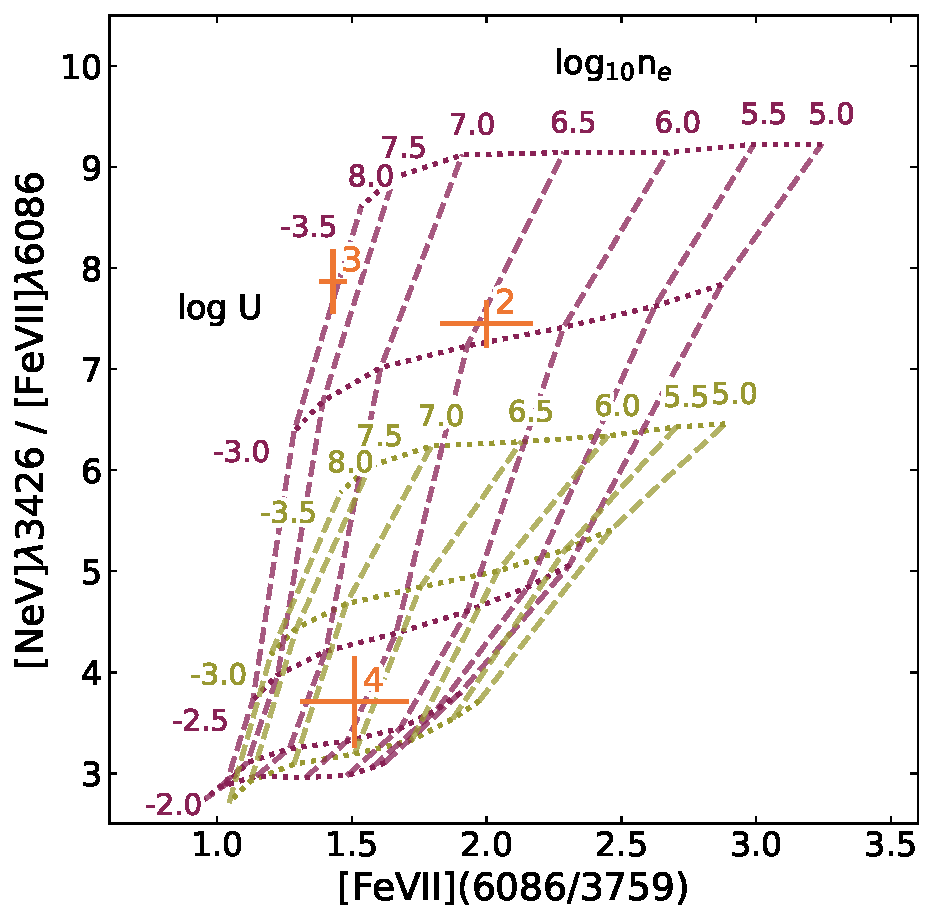
\includegraphics[width=0.7\linewidth]{figures/stis_seyferts/nev_fevii_vary_a.pdf}
    \caption[{[}FeVII{]}(6087/3759) vs {[}NeV{]}$\lambda$3426/{[}FeVII{]}$\lambda$6086 diagnostic diagram for the highly-ionised gas in NGC\;1068, along with grids produced from photoionisation modelling.]{[FeVII](6087/3759) vs [NeV]$\lambda$3426/[FeVII]$\lambda$6086 diagnostic diagram with radiation-bounded AGN-photoionisation grids generated with \textsc{CLOUDY} for two values of spectral index: $\alpha=1.0$ (green) and $\alpha=1.5$ (purple). Dashed lines connect points of constant density (labelled), and dotted lines connect points of constant ionisation parameter (also labelled). The measured ratio values in the NGC\;1068 apertures are shown in orange and labelled; from the $\alpha=1.5$ grid, the high-ionisation gas in NGC\;1068 is found to have densities in the range 6.45\;\textless\;log$_{10}$($n_e$\;[cm$^{-3}$])\;\textless\;8.00.}
    \label{fig: stis_seyferts: nev_fevii_a_vary}
\end{figure}

\vspace*{\fill}

\newpage
\subsection{Energetics of the outflowing gas}
\label{section: stis_seyferts: energetics}

\subsubsection{Outflow kinematics}
\label{section: stis_seyferts: kinematics}

Determining the mass outflow rates, kinetic powers, and coupling efficiencies of the gas outflows detected in the STIS spectra required measurements of the kinematics of the outflowing gas\footnote{Kinematics were not derived from the [OIII] models produced here due to the relatively-low spectral resolution and high instrumental widths of the G430L and G750L spectra.}. For this purpose, the results from detailed kinematic modelling of the NLRs of NGC\;1068 and NGC\;4151 presented by \citet{Crenshaw2000_N1068} and \citet{Crenshaw2000_N4151} (hereafter CKN1068 and CKN4151), respectively, were used. I note that, due to the different PAs used and the fact that the outflow geometry likely depends greatly on PA, the updated kinematic models from \citet{Das2005} and \citet{Das2006} were not used. 

To calculate deprojected velocities, a universal `deprojection factor' was first derived by dividing the maximum observed velocities (located at the velocity `turnover' position: see \citealt{Crenshaw2000_N1068} and \citealt{Crenshaw2000_N4151}) by the maximum model-deprojected velocities from the CKN1068 and CKN4151 bicone models. The highest observed (projected) velocity at the position of each aperture was taken and divided by the determined deprojection factor to give the maximum deprojected outflow velocity in each aperture. The deprojected outflow velocities are given in Table \ref{tab: energetics}, and are hereafter labelled as $v_\mathrm{out}$. 

\textbf{I note that, while the aperture widths were not deprojected (as this projection factor would be highly uncertain), this would not have a significant effect on the conclusions and interpretations made in this chapter: the assumed outflow velocities (which are taken to be the maximal velocities from the bicone models) compensate for the lack of any (likely modest) aperture-width deprojection when calculating mass outflow rates and kinetic powers.}

\subsubsection{Mass outflow rates, kinetic powers, and coupling efficiencies}
\label{section: stis_seyferts: mout_ekin_fkin}

H$\mathrm{\beta}$ luminosities were used to determine masses for the warm-ionised gas in each aperture with Equation \ref{eq: introduction: outflows: energetics: mout}; the Case B recombination coefficient for H$\mathrm{\beta}$ was taken to be $\alpha^{eff}_{H\beta}=1.61\times10^{-14}$\;cm$^3$\;s$^{-1}$ (for a gas of density $n_e=10^4$\;cm$^{-3}$ and temperature $T_e=20,000$\;K: \citealt{Osterbrock2006}). Assuming that the derived masses (estimated using the total line fluxes) are dominated by outflowing gas, they were combined with the outflow velocities from the CKN1068 and CKN4151 models ($v_\mathrm{out}$) and the aperture widths ($\Delta R$) to calculate mass outflow rates using Equation \ref{eq: introduction: outflows: energetics: mout_rate}. The resulting mass outflow rates were then used to produce kinetic powers with Equation \ref{eq: introduction: outflows: energetics: ekin}.

Finally, the ratio of the kinetic power to the bolometric AGN luminosity was taken to estimate coupling efficiencies for each aperture (Equation \ref{eq: introduction: outflows: introduction: e_f}). NGC\;1068 has a bolometric luminosity in the range 0.4\;\textless\;$L_\mathrm{bol}$\textless\;4.7$\times10^{45}$\;erg\;s$^{-1}$ \citep{Woo2002, AlonsoHerrero2011, LopezRodriguez2018, Gravity2020}, of which the lowest value is taken to ensure higher estimates of coupling efficiencies and thus determine the maximum potential impact of the outflowing gas on the host galaxy. For NGC\;4151, the bolometric luminosity was taken to be $L_\mathrm{bol}=1.4\times10^{44}$\;erg\;s$^{-1}$ \citep{Kraemer2020}.

Derived mass outflow rates, kinetic powers and coupling efficiencies for NGC\;1068 and NGC\;4151 are presented in Table \ref{tab: energetics}. For NGC\;1068, the maximum values determined here ($\dot{M}_\mathrm{out}=3.7\pm0.6$\;M$_\odot$\;yr$^{-1}$; $\dot{E}_\mathrm{kin}=(2.0\pm0.3)\times10^{42}$\;erg\;s$^{-1}$, $\epsilon_\mathrm{f}=0.49\pm0.07$\;per\;cent) are less than the maximum values determined from photoionisation modelling by \citet{Revalski2021}\footnote{\citet{Crenshaw2015} and \citet{Revalski2021} assume bolometric luminosities of $L_\mathrm{bol}=1\times10^{45}$\;erg\;s$^{-1}$ for NGC\;1068 and $L_\mathrm{bol}=7.9\times10^{43}$\;erg\;s$^{-1}$ for NGC\;4151 when calculating coupling efficiencies.}. For NGC\;4151, the maximum derived values ($\dot{M}_\mathrm{out}=6.9\pm1.8$\;M$_\odot$\;yr$^{-1}$; $\dot{E}_\mathrm{kin}=(1.4\pm1.0)\times10^{42}$\;erg\;s$^{-1}$,  $\epsilon_\mathrm{f}=0.99\pm0.26$\;per\;cent) are similar to the results of photoionisation modelling by \citet{Crenshaw2015}. The mass outflow rates for NGC\;4151 calculated here are also consistent with previous values derived for the warm ionised phase by \citet{Storchi-Bergmann2010} ($\dot{M}_\mathrm{out}\approx2.4$\;M$_\odot$\;yr$^{-1}$) and the X-ray emitting gas ($\dot{M}_\mathrm{out}\approx2$\;M$_\odot$\;yr$^{-1}$: \citealt{Wang2011} and \citealt{Kraemer2020}).

For NGC\;1068, the mass outflow rates for the warm ionised phase are much below that of the cold-molecular gas at a similar radial distance from the nucleus (i.e. traced by CO, HCN; $T\sim100$\;K): \citet{GarciaBurillo2014} derive a cold-molecular mass outflow rate of $\dot{M}_\mathrm{out}=63^{+21}_{-37}$\;M$_\odot$\;yr$^{-1}$ within the $r\sim200$\;pc circumnuclear disk (CND) of NGC\;1068. This indicates that most of the outflowing mass may be present in the colder, non-ionised gas phases, as has been found for other objects (see Chapter \ref{chapter: xshooter_ic5063} and \citealt{RamosAlmeida2019}).

\begin{table*}
    \renewcommand{\arraystretch}{1.2}
    \setlength{\tabcolsep}{5.5pt}
    \centering
    \begin{tabular}{cccccc}
    \multirow{2}{*}{Aperture} & $v_\mathrm{out}$ & $M_\mathrm{out}$ &  $\dot{M}_\mathrm{out}$ & \multirow{2}{*}{$\dot{E}_\mathrm{kin}$ (erg\;s$^{-1}$)}  & \multirow{2}{*}{$\epsilon_\mathrm{f}$ (per\;cent)} \\ 
        &   (km\;s$^{-1}$) & (M$_\odot$) & (M$_\odot$yr$^{-1}$) & & \\
    \multicolumn{6}{c}{\vspace{-0.4cm}} \\
    \multicolumn{6}{c}{NGC 1068} \\ \hline
    1 & -1300 & $1.7\pm0.3$ & $3.7\pm0.6$ & $(2.0\pm0.3)\times10^{42}$ & $(4.9\pm0.7)\times10^{-1}$    \\
    2 & -1100 & $0.63\pm0.08$ & $1.6\pm0.2$ & $(6.1\pm0.7)\times10^{41}$ & $(1.5\pm0.2)\times10^{-1}$ \\
    3 & -450 & $0.73\pm0.09$ & $1.2\pm0.1$ & $(7.6\pm0.9)\times10^{40}$ & $(1.9\pm0.2)\times10^{-2}$    \\
    4 & -150 & $0.94\pm0.22$ & $0.60\pm0.14$ & $(4.2\pm1.0)\times10^{39}$ & $(1.1\pm0.2)\times10^{-3}$    \\ 
    \multicolumn{6}{c}{\vspace{-0.4cm}} \\
    \multicolumn{6}{c}{NGC 4151}    \\ \hline
    1 & -700 & $2.5\pm0.6$ & $3.7\pm1.0$ & $(5.8\pm0.2)\times10^{41}$ & $(4.1\pm1.1)\times10^{-1}$    \\
    3 & -800 & $0.72\pm0.30$ & $3.4\pm1.4$ & $(6.9\pm2.9)\times10^{41}$ & $(4.9\pm2.0)\times10^{-1}$    \\
    5 & 800 & $1.7\pm0.4$ & $4.5\pm1.2$ & $(9.2\pm2.4)\times10^{41}$ & $(6.5\pm1.7)\times10^{-1}$ \\
    6 & 800 & $2.9\pm0.7$ & $6.9\pm1.8$ & $(1.4\pm0.4)\times10^{42}$ & $(9.9\pm2.6)\times10^{-1}$    \\ 
    \end{tabular}
    \caption[Outflow velocities, outflow masses, mass outflow rates, kinetic powers, and coupling efficiencies for the apertures of the STIS spectra of NGC\;1068 and NGC\;4151.]{Outflow velocities, outflow masses, mass outflow rates, kinetic powers, and coupling efficiencies for the apertures of the STIS spectra of NGC\;1068 and NGC\;4151. The outflow velocities used to calculate the mass outflow rates and kinetic powers presented here are from the CKN1068 and CKN4151 models (see Section\;\ref{section: stis_seyferts: kinematics}).}
    \label{tab: energetics}
\end{table*}


\newpage
\section{Discussion}
\label{section: stis_seyferts: discussion}

Through the analysis of archival STIS spectra of the central regions ($r$\;\textless\;160\;pc) of NGC\;1068 and NGC\;4151, this chapter has presented evidence for dense (10$^{3.6}$\;\textless\;$n_e$\;\textless\;10$^{4.8}$\;cm$^{-3}$) gas that shows line ratios consistent with matter-bounded AGN-photoionisation in the case of NGC\;1068, and shock-ionisation (with precursor gas ionisation) or radiation-bounded AGN-photoionisation in the case of NGC\;4151. Furthermore, the measured H$\mathrm{\beta}$ luminosities could be explained as being due to shock-ionisation for both objects, assuming a shock covering factor of unity. In both objects, outflow coupling efficiencies are derived that are close to the lowest value required by models of galaxy evolution, however, these are likely underestimates. In this section, I discuss the implication of these results on the dominant ionisation and acceleration mechanisms of the gas seen in the STIS slits, compare the results of this analysis to past work on these two well-studied objects, and investigate the impact on the density diagnostic techniques used. Finally, I place the results of this chapter in a broader context by comparing them with those of Chapter \ref{chapter: xshooter_ic5063}, which considered the Seyfert 2 galaxy IC\;5063.

\subsection{The outflow ionisation and acceleration mechanisms in the NLRs of NGC 1068 and NGC 4151}
\label{section: stis_seyferts: disc-ionisation}

To determine the true impact of the outflowing gas on the host galaxies, quantitative comparison of observations to theoretical modelling is needed. However, both modelling of jet-ISM interactions  \citep{Capetti1997, Axon1998, May2017, May2020} and radiation-pressure-driven outflows \citep{Crenshaw2000_N4151, Crenshaw2000_N1068, Das2005, Das2006, Revalski2021, Meena2023} is able to explain the observed kinematics in NGC\;1068 and NGC\;4151. Therefore, in order to enable accurate comparisons to theoretical models and thus accurately determine the impact of the outflows in these objects, the dominant outflow acceleration mechanism(s) need to be robustly identified.

\subsubsection{Matter-bounded ionisation and the acceleration mechanism in NGC 1068}

It has been previously proposed that the outflows in NGC\;1068 are driven via radiation pressure \citep{Kraemer2000II, Das2006, Revalski2021, Meena2023}, instead of via shocks induced by the radio jet colliding with the ISM within the bicone. While emission from the outflowing and quiescent gas is not separated in this work, the results presented here may be taken as consistent with this mechanism: Section\;\ref{section: stis_seyferts: mechanisms} presents evidence for matter-bounded AGN-photoionisation of the warm-ionised gas in the form of simultaneous high [OIII] temperatures (Table \ref{tab: stis_seyferts: ne_ebv_te}: $T_e\sim15,000$\;K; corresponding to [OIII](5007/4363)\;\textless\;60) and line ratios (\mbox{HeII$\lambda$4686\;/\;H$\mathrm{\beta}$\;\textgreater\;0.4}: Figure\;\ref{fig: stis_seyferts: oiii_heii_hbeta_stis}; \mbox{[NeV]$\lambda3426$\;/\;[NeIII]$\lambda$3869\;\textgreater\;1.0}: Figure\;\ref{fig: stis_seyferts:nev_neiii_heii_hbeta_stis}) within a 134\;pc radius from the nucleus in the NE cone along the radio axis, as perhaps may be expected for radiatively-accelerated gas. However, it is possible that the outflowing gas has been shock-ionised and accelerated by the jet, but has subsequently cooled and then been reionised by the AGN (as is the case for IC\;5063: Chapter \ref{chapter: xshooter_ic5063}). Spatially-resolved, high spectral-resolution observations are needed to further investigate this situation by separating the emission from the outflowing and quiescent gas, and then determining the ionisation and excitation mechanisms of each kinematic component. In addition, comparing the electron densities of the outflowing and non-outflowing gas may reveal signs of shock compression, which is expected to be a factor of $\sim$4--100 \citep{Sutherland2017}.

It is notable that the outflowing gas in NGC\;1068 appears to be spatially confined to the extent of the radio structure: the broad (FWHM\;\textgreater\;250\;km\;s$^{-1}$) [OIII]$\lambda\lambda$4959,5007 emission in the G430L spectra is seen to a maximum radius of $\sim$4.8\;arcseconds from the nucleus in the NE cone (as measured from the line profiles of the [OIII] emission that extends beyond the regions covered by the apertures), similar to the maximum radial extent of the NE radio lobe (6.18\;arcseconds; 420\;pc) measured from radio imaging (e.g. 15\;GHz: \citealt{WilsonUlvestad1987}; 5\;GHz: \citealt{Wilson1983}, \citealt{Gallimore1996}; 22\;GHz: \citealt{Gallimore1996}; 1.4\;GHz: \citealt{Gallimore1996}, \citealt{GarciaBurillo2014}). This is also in agreement with ground-based Fabry-Pérot integral field spectroscopy by \citet{Cecil1990} --- which finds no significant velocity deviation from the systematic velocity beyond the radio lobe --- and kinematic modelling by \citet{Crenshaw2000_N1068}, \citet{Das2006} and \citet{Meena2023}, who find outflows extended up to a radial distance of $\sim$5.1\;arcseconds from the nucleus\footnote{An [OIII] emission knot in the NLR of NGC\;1068, labelled `A' by \citet{Meena2023} and located 7.3\;arcseconds from the nucleus (i.e. beyond the radio source), has outflow-like kinematics (200\;\textless\;FWHM\;\textless\;1000\;km\;s$^{-1}$; $v_\mathrm{out}=863$\;km\;s$^{-1}$). As noted by \citet{Meena2023}, this knot lies beyond the expected extent of radiatively-driven outflows. Regardless, I highlight that the vast majority of the outflows along the radio axis are located at lower radii than the maximum extent of the NE radio lobe.}. Furthermore, VLT/MUSE spectroscopy presented by \citet{Venturi2021} shows that the measured [OIII] $W_\mathrm{70}$ velocity parameter has high values \mbox{(400\;\textless\;[OIII]\;$W_\mathrm{70}$\;\textless\;1200\;km\;s$^{-1}$)} between the nucleus and the lobe, out to a radius of 3.6\;arcseconds along the bicone axis. Moreover, the NLR molecular CO(3--2) outflows (as seen in ALMA imaging by \citealt{GarciaBurillo2014}) decelerate within the radio lobe, at a distance of $r\sim400$\;pc ($r\sim5.7$\;arcseconds) from the nucleus. Taken together, this shows that the NE cone outflows have a similar extent to the NE radio lobe, and is evidence for the outflows being accelerated by the radio jet, although it does not entirely rule out radiative acceleration.

\subsubsection{Shock-ionisation and acceleration in NGC 4151}

The results produced here for NGC\;4151 indicate that the near-nuclear gas along the radio axis may be shock-ionised, since the measured [OIII](5007/4363), HeII/H$\mathrm{\beta}$, and [NeV]$\lambda$3426/[NeIII]$\lambda$3869 line ratios and H$\mathrm{\beta}$ luminosities are consistent with those expected from a mixture of pure-shock and shock-precursor ionisation (Figures \ref{fig: stis_seyferts: oiii_heii_hbeta_stis} and \ref{fig: stis_seyferts:nev_neiii_heii_hbeta_stis}; Section\;\ref{section: stis_seyferts: shock_viability}).

The radio structure in the NLR of NGC\;4151, as seen in low-resolution 1.5--5\;GHz VLA radio imaging by \citet{Johnston1982}, has a lobe-like component with a centroid 6.43\;arcseconds from the nucleus along the radio axis in the NE cone. This structure lies beyond the maximum $\sim$4\;arcseconds extent of the warm-ionised outflows (\citealt{Meena2023}; see also \citealt{Das2005}), and --- as I have argued for the situation in NGC\;1068 --- is consistent with the outflows being launched by the radio jet. From HST/PC + HST/WFPC2 imaging, \citet{Williams2017} found higher [OIII]/H$\mathrm{\alpha}$ ratios close to the string of radio knots that are seen in their higher-resolution 1.51\;GHz observations (shown here in Figure\;\ref{fig: observations_and_data_reduction: stis_seyferts: observations: seyferts_wfpc2}), with the values of this ratio decreasing beyond radial distances of $r\sim4$\;arcseconds from the nucleus along the radio axis. The authors interpreted this as the radio jet having a contribution to the ionisation of the gas close to the nucleus, but AGN-photoionisation being dominant further out. This is also in agreement with the results from X-ray and optical imaging by \citet{Wang2011b}, who propose a mixture of shock-ionisation and AGN-photoionisation in the NLR of NGC\;4151. 

Taken together with the findings of these previous investigations, the results presented in this chapter may indicate that the outflows in NGC\;4151 have been shock-accelerated and then re-ionised by photons from the AGN in varying amounts at different locations, with AGN-photoionisation being dominant further from the nucleus.


\subsection{The effect of ionisation mechanisms on density diagnostics}
\label{section: stis_seyferts: disc-density-effects}

The ionisation mechanisms (Section\;\ref{section: stis_seyferts: mechanisms}), electron temperatures (Section\;\ref{section: stis_seyferts: electron_temperatures}), and electron densities (Sections \ref{section: stis_seyferts: tr_diagnostics} and \ref{section: stis_seyferts: high_ionisation}) of the warm-ionised gas detected in the STIS slits allow an investigation into the structures and conditions of the line-emitting clouds, and therefore verification of the origins of different emission lines and the precision of diagnostics which make use of them. For example, the transauroral-line density diagnostic (Section\;\ref{section: stis_seyferts: tr_diagnostics}) relies on AGN-photoionisation being dominant, with no significant contribution from a matter-bounded component or shock-ionisation. Since evidence is found here for matter-bounded emission in NGC\;1068 and potential shock-ionisation in NGC\;4151, it is important to investigate the effect of this on derived densities.

\subsubsection{The impact of matter-bounded photoionisation}
\label{section: stis_seyferts: disc-density-mb}

If the higher-ionisation lines are indeed emitted by matter-bounded gas structures in the outflow (as shown by the [OIII] temperatures, HeII/H$\mathrm{\beta}$ ratios, and [FeVII](6086/3759) vs [NeV]$\lambda$3426/[FeVII]$\lambda$6086 diagram: Sections \ref{section: stis_seyferts: mechanisms} and \ref{section: stis_seyferts: high_ionisation}), then the transauroral lines cannot be emitted by these structures. However, it is possible that they are emitted by different clouds within the same cloud complexes, considering that these lines have similar profiles in each of the apertures. Alternatively, or perhaps in addition, it is possible that the outer layers of a single cloud are matter-bounded, while the denser core is radiation-bounded (one of the scenarios presented by \citealt{Binette1996}). In this scenario, the matter-bounded layers may represent lower-density gas that was driven away from the ionisation front by the increase in pressure that occurred when the gas structure was first photoionised by the AGN. However, this is not consistent with findings of this chapter: in Section\;\ref{section: stis_seyferts: high_ionisation}, the [FeVII](6087/3759) and [NeV]$\lambda$3426/[FeVII]$\lambda$6086 emission-line ratios were used to determine high-ionisation gas densities of 6.45\;\textless\;log$_{10}$($n_e$\;[cm$^{-3}$])\;\textless\;8.00 in the NGC\;1068 apertures: significantly higher than that of the lower-ionisation gas. A potential explanation is that the gas that is emitting the high-ionisation [FeVII] and [NeV] lines represents dense fragments of the expanding matter-bounded component: since these lines have high critical densities (7.1\;\textless\;log$_{10}(n_\mathrm{crit}$\;[cm$^{-3}$])\;\textless\;8.5; Appendix \ref{appendix: properties_of_warm_ionised_diagnostic_lines}), they would only be emitted strongly by such dense cloud components.

Therefore, given the ionisation energies of the lines (Appendix \ref{appendix: properties_of_warm_ionised_diagnostic_lines}), I propose that the [FeVII] and [NeV] lines trace matter-bounded, higher-ionisation clouds within the complexes (or edges of individual clouds), and the [OII] and [SII] lines are emitted from radiation-bounded clouds (or cores of individual clouds). In this scenario, much of the [OIII] emission must arise from the matter-bounded regime in order to explain the high electron temperatures that are measured in the NGC\;1068 apertures (Section\;\ref{section: stis_seyferts: electron_temperatures}). Hence, given the high density of the high-ionisation gas, it is likely that the gas emitting the [OIII] lines is denser than the gas that is emitting the transauroral lines. This reinforces the need for outflow diagnostics that are sensitive to high ($n_e$\;\textgreater\;10$^{3.5}$\;cm$^{-3}$) densities.

\subsubsection{The impact of shock-ionisation}

Since the gas in the NGC\;4151 apertures may be shock-ionised, it is essential to quantify the effect of this on the transauroral-ratio density diagnostic. In Appendix \ref{appendix: tr_grid_shock_modelling}, I plot the TR ratios from shock models over the transauroral-line photoionisation diagnostic grid used in Section\;\ref{section: stis_seyferts: tr_diagnostics}, and quantify the impact of shock-ionisation on the transauroral-line-derived electron density and reddening values. These diagrams show that, overall, the effect on the derived density is $\pm$0.38 orders of magnitude, and the effect on derived reddening values is E(B-V)$\pm$0.13. Crucially, this is much less than the impact of using lower-critical-density techniques (such as the [SII](6717/6731) ratio), and is similar to the effect of varying the parameters of the photoionisation model (\citealt{Santoro2020}: log($n_e$[cm$^{-3}$])$\pm$(0.1--0.7); E(B-V)$\pm$(0.1--0.2)). In summary, while using the transauroral-line method presented by \citet{Holt2011} as a density and reddening diagnostic for shock-ionised gas does incur some uncertainty on the derived densities, the derived densities are still likely more accurate than those derived from commonly-used, traditional methods.

Gas that has been shock-ionised by jet-ISM interactions presents a problem for the photoionisation modelling method used by \citet{Revalski2021}, as the technique relies on assuming that material at a given distance from the nucleus is being photoionised by the central AGN engine. In the case of shock-ionisation, the outflows are instead being shock-ionised \textit{locally} within the bicone at any given distance from the nucleus, and so any electron densities derived using an assumed ionisation parameter and distance will be incorrect. \citet{Revalski2021} used the standard BPT diagrams \citep{Baldwin1981} in an attempt to ensure all of the measured line ratios were consistent with AGN-photoionisation. However, the regions of AGN shock and photoionisation in these diagrams overlap considerably (Section\;\ref{section: introduction: outflows: accleration_mechanisms: ionisation_and_excitation_mechanisms}); further diagnostics should also be used in order to disentangle the contribution from shocks and photoionisation, such as the [OIII](5007/4363) vs HeII$\lambda$4686/H$\mathrm{\beta}$ (\citealt{VillarMartin1999}; used in this chapter in Figure \ref{fig: stis_seyferts: oiii_heii_hbeta_stis}) and [FeII]$\lambda$12570/Pa$\mathrm{\beta}$ vs H$_2\lambda$21218/Br$\mathrm{\gamma}$ (Chapter \ref{chapter: xshooter_ic5063}, Figure \ref{fig: xshooter_ic5063: feii_pab}; \citealt{Rodriguez-Ardila2005, Riffel2013a, Colina2015, Riffel2021}) diagnostic diagrams, and/or the three-dimensional diagram (which makes use of line ratios and velocity dispersion) presented by \citet{DAgostino2019}.

Overall, despite the challenges that shock-ionisation and significant-matter-bounded photoionisation components present to the transauroral-line technique and the \citet{Revalski2021} photoionisation modelling, I argue that these methods are nonetheless more-robust density diagnostics than the commonly-used [SII](6717/6731) and [OII](3726/3729) ratios. In the case of matter-bounded photoionisation, the [SII]$\lambda\lambda$6717,6731 and [OII]$\lambda\lambda$3726,3729 lines arise from the same part of the ionisation structure of the cloud as the transauroral lines, meaning they face the same issues as the transauroral-line method, while the \citet{Revalski2021} modelling allows for higher-ionisation components, and therefore is a more-accurate diagnostic of the overall cloud density. Furthermore, it is established here that using radiation-bounded photoionisation grids to measure the densities of shock-ionised gas with the transauroral-line method incurs an uncertainty on the overall density that is much less than using lower-critical density line ratios for high-density ($n_e$\;\textgreater\;10$^{3}$\;cm$^{-3}$) gas: in the case of NGC\;4151 (where there may be some contribution from shock-ionisation), the transauroral-line-derived densities are similar to those reported by \citet{Revalski2022} (see also \citealt{Crenshaw2015}), indicating that both methods still give more-precise density determinations than traditional methods, despite some of their underlying assumptions potentially being incorrect.

\subsubsection{The origin of the transauroral lines in NGC 1068, NGC 4151 and IC 5063}

In order to further investigate the origin of the transauroral lines in the archetypal Seyfert galaxies (and the nearby Sey 2 IC\;5063: Chapter \ref{chapter: xshooter_ic5063}), the measured [OII](7319+7331)/[OIII]$\lambda$5007 vs [SII](4068+4076)/H$\mathrm{\beta}$ ratios are plotted with overlaid grids from radiation-bounded photoionisation modelling (as first presented by \citealt{Spence2018}) and shock modelling in Figures \ref{fig: stis_seyferts: tr_oiii_hbeta}a and \ref{fig: stis_seyferts: tr_oiii_hbeta}b, respectively. 

The photoionisation models in Figure\;\ref{fig: stis_seyferts: tr_oiii_hbeta}a are those used in Sections \ref{section: stis_seyferts: tr_diagnostics} and \ref{section: stis_seyferts: mechanisms}, generated using \textsc{CLOUDY} for a radiation-bounded cloud with varying values of density, ionisation parameter and spectral index. The measured ratios for NGC\;1068 and NGC\;4151 are consistent with this grid; however, the corresponding ionisation parameters are a half-an-order-of-magnitude higher than that which was required to reproduce the measured transauroral-line ratios (log\;$U=-3$; Figure\;\ref{fig: stis_seyferts: tr_ddd}). This is further evidence that radiation-bounded AGN-photoionisation is not the dominant ionisation mechanism in the STIS apertures, and in the case of NGC\;1068, can be explained as the [OIII] and H$\mathrm{\beta}$ emission being dominated by matter-bounded components (as indicated by the measured HeII/H$\mathrm{\beta}$ ratios; Figure\;\ref{fig: stis_seyferts: oiii_heii_hbeta_stis}). This is because matter-bounded emission will increase the relative strength of the [OIII] and H$\mathrm{\beta}$ lines, reducing the [OII](7319+7331)/[OIII]$\lambda$5007 and [SII](4068+4076)/H$\mathrm{\beta}$ ratios and thus giving a higher corresponding ionisation parameter on the radiation-bounded grid.

These measured ratios are also presented in Figure\;\ref{fig: stis_seyferts: tr_oiii_hbeta}b with the expected ratios from shock-ionisation modelling. The shock models here are those presented by \citet{Allen2008}, and are for two values of pre-shock density (10$^1$\;cm$^{-3}$ and 10$^2$\;cm$^{-3}$), velocities of $v_\mathrm{shock}=400, 600, 800$\;km\;s$^{-1}$, and magnetic parameters in the range 2\;\textless\;$B/\sqrt{n}$\;\textless\;10\;$\mu$G\;cm$^{3/2}$. In all apertures for NGC\;4151, the measured line ratios are consistent with shock-ionisation, albeit with relatively-high magnetic parameters (4\;\textless\;$B/\sqrt{n}$\;\textless\;10\;$\mu$G\;cm$^{3/2}$). These magnetic parameters are higher than those typical for the ISM (2\;\textless\;$B/\sqrt{n}$\;\textless\;4\;$\mu$G\;cm$^{3/2}$; \citealt{Dopita1995, Allen2008}), potentially indicating higher magnetic fields associated with the shocked material. If the gas detected in the NGC\;4151 data is indeed shock-ionised, then the position of the shock-model grid on the diagram would explain why the ionisation parameter deduced from the radiation-bounded photoionisation grid (Figure\;\ref{fig: stis_seyferts: tr_oiii_hbeta}a) for the NGC\;4151 apertures is higher than expected from the TR diagnostic grid (Figure\;\ref{fig: stis_seyferts: tr_ddd}): shock-ionisation produces lower values of [OII](7319+7331)/[OIII]$\lambda$5007 and [SII](4068+4076)/H$\mathrm{\beta}$, corresponding to higher ionisation parameters on the photoionisation grid.

Finally, I also present [OII](7319+7331)/[OIII]$\lambda$5007 and [SII](4068+4076)/H$\mathrm{\beta}$ ratios for the Seyfert 2 galaxy IC\;5063, as measured from the VLT/Xshooter dataset described in Chapter \ref{chapter: xshooter_ic5063}. In agreement with the analysis of Chapter \ref{chapter: xshooter_ic5063}, here it is found that the ratios are consistent with radiation-bounded AGN-photoionisation for an ionisation parameter of $-3$\;\textless\;log\;$U$\;\textless\;$-2$ and densities in the range 3\;\textless\;log$_{10}(n_e$[cm$^{-3}$])\;\textless\;4.

\begin{figure*}[!t]
    \centering
    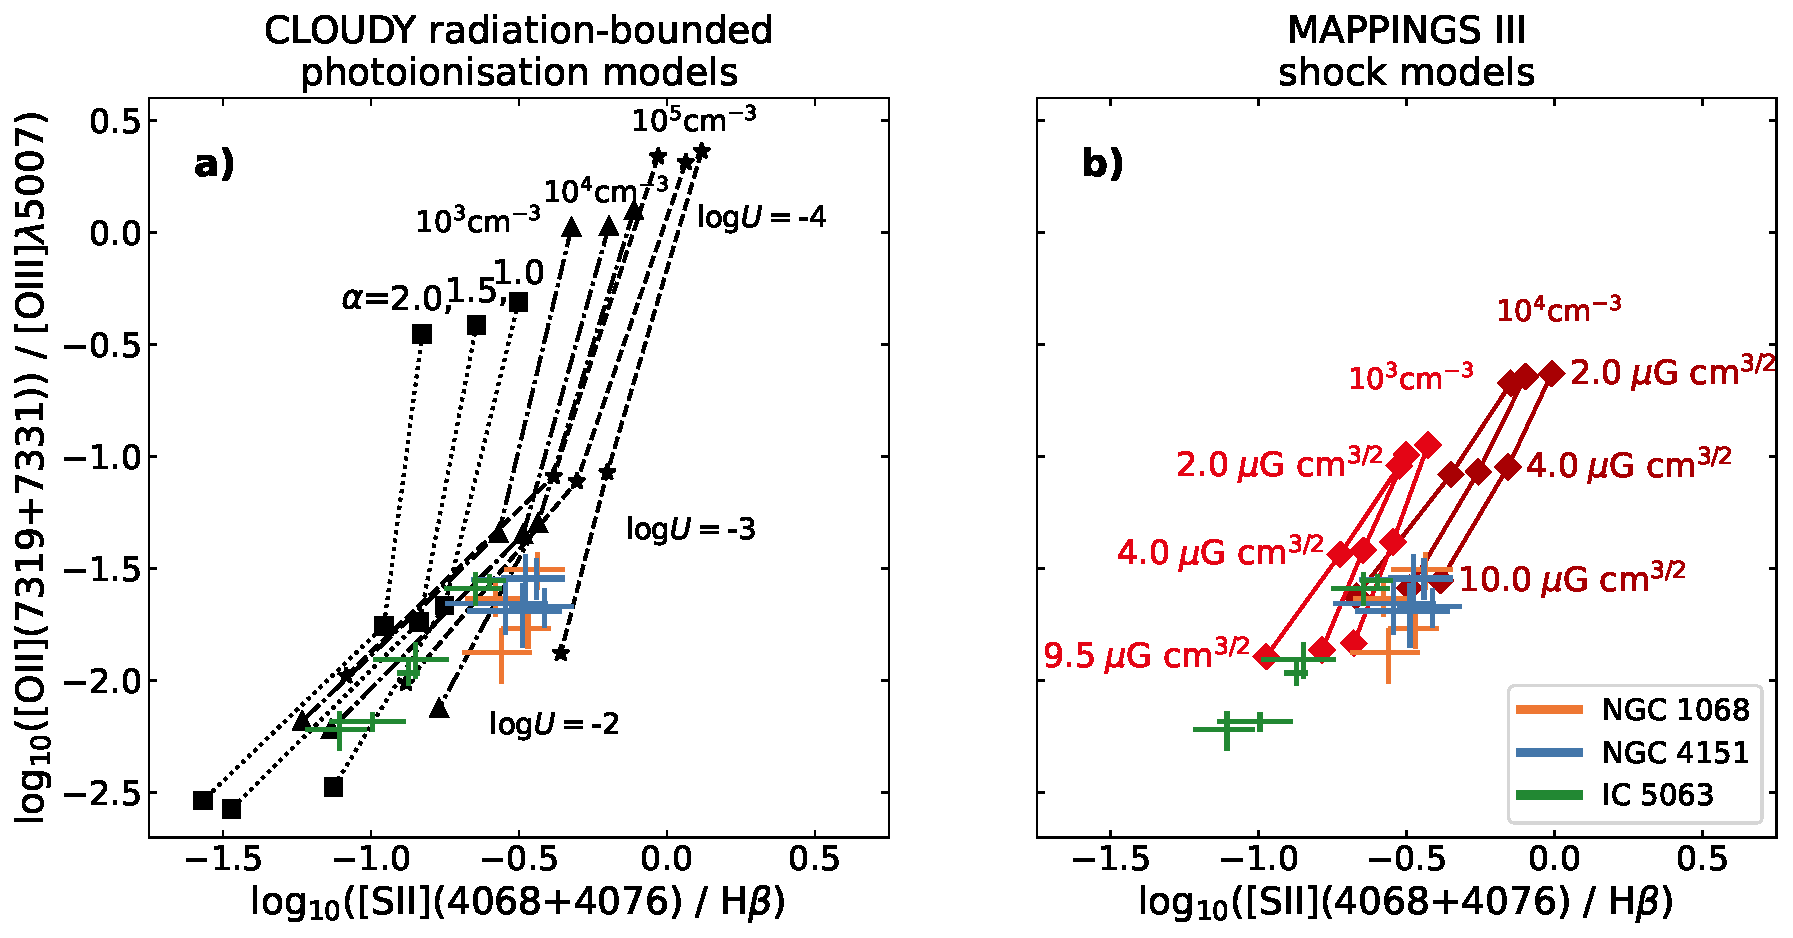
\includegraphics[width=\linewidth]{figures/stis_seyferts/tr_oiii_hbeta.pdf}
    \caption[TR({[}SII{]})/H$\mathrm{\beta}$ vs TR({[}OII{]})/{[}OIII{]}$\lambda$5007 diagnostic diagram for the warm ionised gas in IC\;5063, NGC\;1068, and NGC\;4151, along with grids produced from photo- and shock-ionisation modelling.]{TR([SII])/H$\mathrm{\beta}$ vs TR([OII])/[OIII]$\lambda$5007 ratio grids from \textsc{CLOUDY} radiation-bounded photoionisation modelling (\textbf{a}) and the \citet{Allen2008} MAPPINGS III shock-ionisation models (\textbf{b}), along with measured values for each aperture in NGC\;1068 (orange crosses), NGC\;4151 (blue crosses) and IC\;5063 (green crosses; see Chapter \ref{chapter: xshooter_ic5063}). The modelled photoionisation-line-ratio grid shown in \textbf{a)} is for three spectral indices ($\alpha=1.0, 1.5, 2.0$; labelled) at different electron densities (squares: $n_e=10^3$\;cm$^{-3}$; triangles: $n_e=10^4$\;cm$^{-3}$; stars: $n_e=10^5$\;cm$^{-3}$) and ionisation parameters (log\;$U$; labelled), while the shock-ionisation grids in \textbf{b)} are for post-shock densities of $n=10^3$\;cm$^{-3}$ and $n=10^{4}$\;cm$^{-3}$ (labelled; assuming a shock compression factor of 100), magnetic parameters of $B/\sqrt{n}=2$, 4, 10 \;$\mu$G\;cm$^{3/2}$ (labelled), and velocities of $v_\mathrm{shock}=400, 600, 800$\;km\;s$^{-1}$.}
    \label{fig: stis_seyferts: tr_oiii_hbeta}
\end{figure*}

\subsection{Comparison of the transauroral-line-derived electron densities to other techniques}
\label{section: stis_seyferts: disc-density-tr}

Using the transauroral-line method, high electron densities are measured for NGC\;1068 (4.00\;\textless\;log($n_e$[cm$^{-3}$])\;\textless\;4.75) and NGC\;4151 (3.50\;\textless\;log($n_e$[cm$^{-3}$])\;\textless\;4.10) (Section\;\ref{section: stis_seyferts: tr_diagnostics}; Table \ref{tab: stis_seyferts: ne_ebv_te}). This agrees with the similarly high densities ($n_e$\;\textgreater\;10$^3$\;cm$^{-3}$) that are derived from multi-component photoionisation modelling of both objects presented in \citet{Crenshaw2015} and \citet{Revalski2021} (see also \citealt{Collins2009} and \citealt{Revalski2022}). Crucially, the derived densities from both techniques lie above the sensitivity range of the traditional [SII](6717/6731) and [OII](3726/2739) techniques, which are commonly used (either directly or as a basis for assumption) to derive electron densities in studies of the warm ionised phase (e.g. \citealt{Nesvadba2006, Liu2013, Harrison2014, Fiore2017}), thus further supporting the need for robust warm-ionised gas electron density diagnostics such as the transauroral-line technique and multi-component photoionisation modelling.

Through the use of the traditional [SII](6717/6731) ratio, \citet{Kraemer2000II} (using the same STIS dataset as used in this work) and \citet{Kakkad2018} and \citet{Mingozzi2019} (using IFU data) derived electron densities of $n_e\sim10^3$\;cm$^{-3}$ for the outflows in the NLR of NGC\;1068. These [SII]-derived densities are 1--1.5 orders of magnitude lower than those that are found using the transauroral-line method, and are close to the upper limit of the density range for the [SII]-ratio technique (Appendix\;\ref{appendix: properties_of_warm_ionised_diagnostic_lines}: $n_{crit}\sim10^{3.5}$\;cm$^{-3}$). This provides further evidence that, for gas of electron densities $n_e$\;\textgreater\;10$^{3.5}$\;cm$^{-3}$, the [SII](6717/6731) ratio may underestimate the true electron density by more than an order of magnitude.

\subsection{The impact of the outflowing gas on the host galaxies}

Using densities derived from the transauroral-line ratios, reddening-corrected recombination line fluxes, and kinematics taken from previous modelling, mass outflow rates in the range 0.6\;\textless\;$\dot{M}_\mathrm{out}$\;\textless\;6.9\;M$_\odot$\;yr$^{-1}$ and coupling efficiencies in the range 1.1$\times10^{-3}$\;\textless\;$\epsilon_\mathrm{kin}$\;\textless\;0.99\;per\;cent are found (Table \ref{tab: energetics}). In many cases, the calculated coupling efficiencies are just above the lower limit required by models of the co-evolution of galaxies and their supermassive black holes (e.g. $\sim0.5$--10\;per\;cent: \citealt{DiMatteo2005, Springel2005, Hopkins2010}). It is important to note that there is likely more outflowing material within the bicones that is not covered by the slits (which are only 0.1\;arcseconds wide), and that comparisons between coupling efficiencies from models and observations are not straightforward (see Section\;\ref{section: introduction: outflows: comparisons_to_models} and \citealt{Harrison2018}). To properly account for the impact of the warm-ionised outflows, detailed studies that make use of robust density diagnostics, separate emission from the outflowing and quiescent gas and, importantly, cover the entire NLRs of both objects, are needed. Moreover, I highlight that assessments of \textit{all} gas phases --- not just the warm ionised phase --- are needed to robustly assess the \textit{total} impact of the AGN-driven outflows (Section\;\ref{section: introduction: outflows: energetics: multi-phase}; \citealt{Cicone2018}), as the warm-ionised gas may represent just a fraction of the total outflowing gas mass at a given radius (e.g. Chapter \ref{chapter: xshooter_ic5063}; \citealt{RamosAlmeida2019}). Therefore, it is likely that the true coupling efficiencies of the total NLR outflows in NGC\;1068 and NGC\;4151 are higher than are calculated here.

\subsection{A tale of three Seyferts: NGC 1068, NGC 4151 and IC 5063}

\begin{table*}
    \vspace*{12pt}
    \centering
    \renewcommand{\arraystretch}{1}
    \begin{tabular}{lccccc}
    \multirow{2}{*}{Object}  & \multirow{2}{*}{$L_\mathrm{bol}$ (erg\;s$^{-1}$)}    & $L_\mathrm{1.4\;GHz}$ & \multirow{2}{*}{$P_\mathrm{jet}$ (erg\;s$^{-1}$)}  & \multirow{2}{*}{$\theta_\mathrm{jet}$$^a$} & \multirow{2}{*}{Ionisation mechanism$^b$} \\ 
        &   & (W\;Hz$^{-1}$)  &   &   & \\ 
        \hline
    \multicolumn{6}{}{\vspace*{-0.2cm}}\\
    \multirow{2}{*}{NGC\;1068} & \multirow{2}{*}{0.4--4.7$\times10^{45}$} & \multirow{2}{*}{2.3$\times10^{23}$}   & \multirow{2}{*}{1.8$\times10^{43}$}   & \multirow{2}{*}{$\sim45^\circ$} & Matter-bounded  \\
        &   &   &   &   &   photoionisation \\
    \multicolumn{6}{}{\vspace*{-1cm}}\\
    \multirow{2}{*}{NGC\;4151} & \multirow{2}{*}{1.4$\times10^{44}$} & \multirow{2}{*}{1.6$\times$10$^{22}$}  & \multirow{2}{*}{$\sim10^{42}$}   & \multirow{2}{*}{$\sim36^\circ$} &  Photo- and/or \\
        &   &   &   &   &   shock-ionisation \\
    \multicolumn{6}{}{\vspace{-1cm}}\\
    \multirow{2}{*}{IC\;5063}  & \multirow{2}{*}{7.6$\times 10^{44}$}  & \multirow{2}{*}{3$\times10^{23}$} & \multirow{2}{*}{10$^{44-45}$} & \multirow{2}{*}{$\sim5^\circ$} & Radiation-bounded \\
        &   &   &   &   &   photoionisation \\
    \multicolumn{6}{}{\vspace{-1cm}}\\
    \end{tabular} \\
    $^a$Jet power for NGC\;1068: \citet{GarciaBurillo2014}; NGC\;4151: \citet{Wang2011b}; IC\;5063: \citet{Mukherjee2018}. \\
    $^b$Determined with line ratios measured in slits along $\mathrm{PA}=202^\circ$ (NGC\;1068), $\mathrm{PA}=70^\circ$ (NGC\;4151) and $\mathrm{PA}=115^\circ$ (IC\;5063). \\
    \caption{Bolometric luminosities, 1.4\;GHz radio luminosities, jet powers ($P_\mathrm{jet}$), jet orientations with respect to the disk ($\theta_\mathrm{jet}$), and ionisation mechanisms determined along the radio axes for the nearby Seyfert galaxies NGC\;1068, NGC\;4151, and IC\;5063.}
    \label{tab: three_seyferts}
\end{table*}

Finally, using the results for the nearby Seyfert 2 IC\;5063 presented in Chapter \ref{chapter: xshooter_ic5063} along with the results for NGC\;1068 and NGC\;4151 that are presented here, a sample of nearby Seyferts with spatially-resolved, detailed studies of their NLR outflows can be constructed.

IC\;5063 is a nearby ($z=0.01131$) early-type Seyfert 2 galaxy that is seen close to edge-on, with a radio jet propagating almost in the plane of the disk which drives fast (\mbox{$v_\mathrm{out}$\;\textgreater\;700\;km\,s$^{-1}$}) outflows (\citealt{Morganti1998, Oosterloo2000, Morganti2015, Mukherjee2018}; Chapter \ref{chapter: xshooter_ic5063}). These outflows are seen in multiple gas phases, including warm ionised (\citealt{Morganti2007, Sharp2010, Congiu2017, Venturi2021}; Chapter \ref{chapter: xshooter_ic5063}), neutral atomic \citep{Morganti1998, Oosterloo2000}, warm molecular (\citealt{Tadhunter2014}; Chapter \ref{chapter: xshooter_ic5063}), and cold molecular \citep{Morganti2013_IC5063, Morganti2015, Dasyra2016, Oosterloo2017}.

In Chapter \ref{chapter: xshooter_ic5063}, I presented evidence that both the outflowing and quiescent warm-ionised gas in IC\;5063 has dominant AGN-photoionisation --- even though the outflows show clear signatures of jet-acceleration --- and that the different outflow phases may represent a post-shock cooling sequence. I interpreted this situation as the pre-shock gas being AGN-photoionised, and the closest post-shock gas to the AGN being maintained in an ionised state by photoionisation. In Figure\;\ref{fig: stis_seyferts: oiii_heii_hb_seyferts}, the [OIII](5007/4363) and HeII4686/H$\mathrm{\beta}$ ratios for the outflowing gas in IC\;5063 (Section\;\ref{section: xshooter_ic5063: properties_of_outflowing_gas: uvb_vis_analysis_and_results: electron_temperatures}) are added to the diagnostic diagram presented in this chapter (Figure\;\ref{fig: stis_seyferts: oiii_heii_hbeta_stis}). Furthermore, [OII](7319+7331)/[OIII]$\lambda$5007 and [SII](4068+4076)/H$\mathrm{\beta}$ ratios for IC\;5063 (alongside NGC\;1068 and NGC\;4151) are presented in Figure\;\ref{fig: stis_seyferts: tr_oiii_hbeta}, determined using the Xshooter data for IC\;5063 --- it can be seen that they are consistent with radiation-bounded AGN-photoionisation with gas densities in the range \mbox{10$^3$\;\textless\;$n_e$\;\textless\;10$^4$\;cm$^{-3}$} and ionisation parameters in the range \mbox{$-3$\;\textless\;log\;$U$\;\textless\;$-2$}, in agreement with the values determined in Chapter \ref{chapter: xshooter_ic5063}. 

\begin{figure}[!t]
\centering
    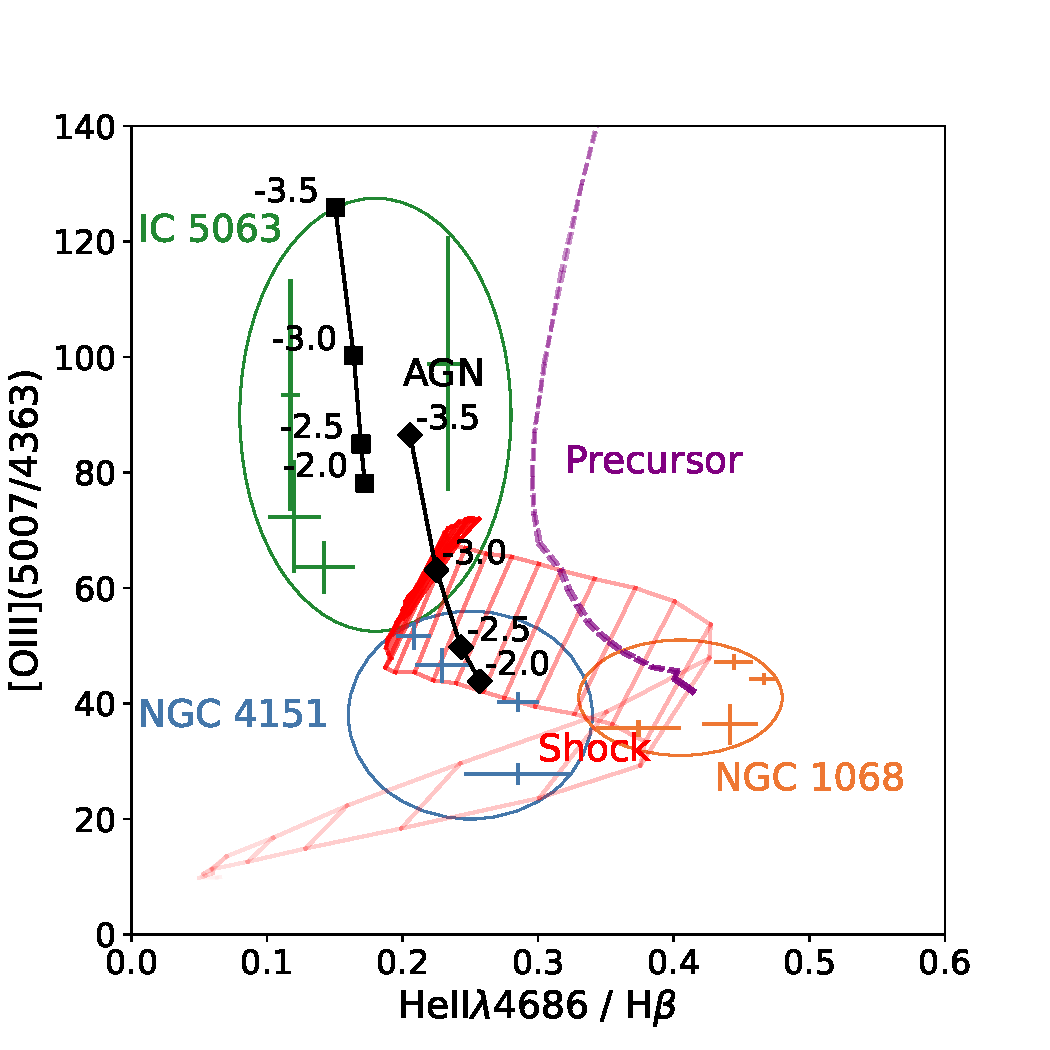
\includegraphics[width=0.8\linewidth]{figures/stis_seyferts/oiii_heii_hb_seyferts.pdf}
    \caption[HeII$\lambda$4686/H$\mathrm{\beta}$ vs {[}OIII{]}5007/{[}OIII{]}$\lambda$4363 diagnostic diagram for the warm ionised gas in IC\;5063, NGC\;1068 and NGC\;4151, including modelled values for (radiation-bounded and matter-bounded) photo- and shock-ionised gas.]{[OIII](5007/4363) vs HeII4686/H$\mathrm{\beta}$ diagnostic diagram (as in Figure\;\ref{fig: stis_seyferts: oiii_heii_hbeta_stis}) with line ratios measured from the STIS spectra of NGC\;1068 and NGC\;4151 (presented in this work), and from Xshooter spectra of IC\;5063 (Chapter \ref{chapter: xshooter_ic5063}, Figure \ref{fig: xshooter_ic5063: heii_hbeta}). The AGN, shock, and precursor models are the same as those described in Section\;\ref{section: stis_seyferts: mechanisms}. The three objects each show distinct ionisation conditions, hinting at the complex nature of the NLRs of Seyfert galaxies.}
    \label{fig: stis_seyferts: oiii_heii_hb_seyferts}
\end{figure}

It is interesting that the overall differences in ionisation conditions \textit{between} the three galaxies are significantly larger than the range of ionisation conditions \textit{within} the galaxies. This small sample thus shows three distinct cases in the three objects: radiation-bounded AGN-photoionisation in IC\;5063, matter-bounded AGN-photoionisation in NGC\;1068, and shock-ionisation or radiation-bounded AGN-photoionisation with a relatively-flat spectral index and higher ionisation parameters in NGC\;4151. Despite all being classified as Seyferts, the details of the ionisation mechanisms in the objects vary greatly. This is particularly interesting considering that in all cases, the outflows detected along the radio axes appear to be spatially confined to the radio structures (i.e. the outflows do not extend beyond the radio lobes in the NLRs). As argued in Section\;\ref{section: stis_seyferts: disc-ionisation}, this is consistent with shock-acceleration, although it does not rule out radiative-acceleration. If the outflows in IC\;5063, NGC\;1068 and NGC\;4151 are shock-accelerated, then this would highlight the importance of not deriving information regarding the outflow acceleration mechanisms based solely on the ionisation/excitation mechanisms or kinematics of the gas in NLRs: a full account, involving detailed multi-wavelength observations with multiple diagnostics, is required to properly evaluate the relative contributions of different mechanisms. 

Despite evidence that the outflows in all three objects are being driven by the radio jet, the densities of the outflowing gas differ by more than an order of magnitude: for IC\;5063, the outflowing gas has densities in the range 3.17\;\textless\;log($n_e$\;[cm$^{-3}$])\;\textless\;3.43 (Table \ref{tab: xshooter_ic5063: densities}), while for NGC\;1068 and NGC\;4151 the densities are in the ranges 4.00\;\textless\;log($n_e$\;[cm$^{-3}$])\;\textless\;4.75 and 3.50\;\textless\;log($n_e$\;[cm$^{-3}$])\;\textless\;4.10, respectively (Table \ref{tab: stis_seyferts: ne_ebv_te}). The reason for this may simply be due to different pre-shock gas densities in the different objects (assuming that the outflows in all three are shock-accelerated): for IC\;5063 the pre-shock density is 2.1\;\textless\;log($n_e$\;[cm$^{-3}$])\;\textless\;2.7, however without higher-velocity-resolution spectra, it is not possible to determine the quiescent gas densities in NGC\;1068 and NGC\;4151. In addition, the differing post-shock densities in the three Seyferts may be due to different cooling conditions behind the shock front. Standard shock-jump conditions predict a compression factor of $\sim$4, however, this may be much higher ($\sim$100) if the post-shock gas has cooled in pressure equilibrium \citep{Sutherland2017, Santoro2018}.

Moreover, it is important to note that all three objects have low-to-intermediate radio luminosities (1.6$\times10^{22}$\;\textless\;$L_\mathrm{1.4\;GHz}$\;\textless\;3.0$\times10^{23}$\;W\;Hz$^{-1}$; Table \ref{tab: three_seyferts}) --- again, if the outflows in these Seyferts are jet-accelerated, then this would reinforce the importance of jet-driven shocks as a feedback mechanism in the inner regions of galaxies, even at lower radio luminosities, in agreement with the statistical study of nearby AGN presented by \citet{Mullaney2013}. Furthermore, the radio jets in NGC\;1068 and NGC\;4151 are oriented out of the galactic disks by $\sim$45$^\circ$ and $\sim$36$^\circ$ respectively, unlike IC\;5063 in which the jet propagates almost directly into the plane of the disk. Therefore, at least within the central few-hundred parsecs of the AGN, this would show that inclined jets can still have an impact on the kinematics and ionisation of the NLR, as predicted by recent relativistic hydrodynamic simulations \citep{Mukherjee2018, Meenakshi2022b}, which show that a jet inclined $\theta_\mathrm{jet}\sim45^\circ$ to the galaxy's disk may have a significant effect on the kinematics, density, and temperature of the gas within the central few kiloparsecs (albeit less so than a jet inclined in the plane of the disk, such as is the case in IC\;5063). Similar hydrodynamic simulations, specifically tailored to the situations in NGC\;1068 and NGC\;4151, could thus be used to quantify the impact of their radio jets on the star-forming gas in their NLRs, as well as the impact of inclined kpc-scale jets in general.

Ultimately, further observations of NGC\;1068 and NGC\;4151 are required to decisively determine the outflow acceleration mechanism(s). Namely, wide-wavelength-coverage spectroscopy (to make available a range of diagnostics) with sufficient velocity resolution to kinematically-discriminate between outflowing (post-shock?) and quiescent (pre-shock?) gas.

\section{Chapter conclusions}
\label{section: stis_seyferts: conclusions}

By analysing archival HST/STIS spectra taken along the radio axes of the inner few hundred parsecs of the NLR of the prototypical Seyfert galaxies NGC\;1068 and NGC\;4151, the following was found.

\begin{itemize}
    \item Spatially-resolved electron densities in the ranges 4.00\;\textless\;log$_{10}(n_e$\;[cm$^{-3}$])\;\textless\;4.75 and 3.60\;\textless\;log$_{10}(n_e$\;[cm$^{-3}$])\;\textless\;4.10  are measured using the transauroral-line technique for the NLR gas in NGC\;1068 and NGC\;4151, respectively. These values are an order of magnitude above those commonly reported and assumed based on traditional density estimates, but are in agreement with the results from alternative diagnostics such as multi-component photoionisation modelling. Overall, these results provide further motivation for the use of the transauroral lines in deriving electron densities of AGN-driven outflows.
    \item The measured emission-line ratios for the warm-ionised gas are consistent with the dominant ionisation mechanisms being matter-bounded AGN-photoionisation in NGC\;1068, and shock-ionisation and/or radiation-bounded AGN-photoionisation with a relatively flat spectral index (and/or higher ionisation parameters and lower metallicities) in NGC\;4151.
    \item Along the radio axes, the outflows in the northeastern cones of both objects have similar spatial extents to the radio structures --- this is consistent with the outflows in their NLRs being shock-accelerated by the radio jets and reionised by radiation from the AGN, although it does not rule out radiative-acceleration.
    \item Applying the transauroral-line technique to gas that has dominant shock-ionisation may incur an uncertainty on the derived electron densities by up to $\pm0.38$ orders of magnitude, which is still far below the potential order-of-magnitude error incurred when using techniques which are not sensitive to higher-density gas. However, care must still be taken when using detailed density-diagnostic techniques, as the ionisation mechanism of the gas may alter the results. Therefore, robust ionisation-mechanism diagnostics should be used to verify the validity of the density measurements.
    \item Finally, combining these findings with those for the nearby Seyfert 2 galaxy IC\;5063 shows that ionisation mechanisms and outflow conditions along the radio axes in the central few hundred parsecs vary significantly between the different objects. Hence, overall, this chapter highlights the necessity of care when deriving information about outflow acceleration mechanisms from the ionisation of the gas, and the need for robust ionisation-mechanism diagnostics with detailed observations.
\end{itemize}

\section*{Chapter acknowledgements}
\addcontentsline{toc}{section}{\protect\numberline{}Chapter acknowledgements}

I thank the anonymous referee for their helpful comments and suggestions, which improved the clarity of the publication that this chapter is based on \citep{HoldenTadhunter2023}. Based on observations made with the NASA/ESA Hubble Space Telescope, and obtained from the Hubble Legacy Archive, which is a collaboration between the Space Telescope Science Institute (STScI/NASA), the Space Telescope European Coordinating Facility (ST-ECF/ESA) and the Canadian Astronomy Data Centre (CADC/NRC/CSA). This research has made use of the NASA/IPAC Infrared Science Archive, which is funded by the National Aeronautics and Space Administration and operated by the California Institute of Technology. This work makes use of the Starlink software \citep{Currie2014}, which is currently supported by the East Asian Observatory. For the purposes of open access, the authors have applied a Creative Commons Attribution (CC BY) licence to any Author Accepted Manuscript Arising.


\section*{Data Availability}
\addcontentsline{toc}{section}{\protect\numberline{}Data availability}

The data used in this chapter is available from the Hubble Legacy Archive (HLA) (\url{https://hla.stsci.edu/hlaview.html}) with proposal IDs GTO:5754 (PI Ford) and GTO:5124 (PI Ford) for the HST/WFPC2 [OIII] imaging, and proposal IDs GTO:7573 (PI Kraemer) and GTO:7569 (PI Hutchings) for the HST/STIS spectra.


\newpage
\thispagestyle{plain}
~\newpage

\chapter{A compact cold-molecular outflow in the ULIRG F13451+1232}
\chaptermark{A compact molecular outflow {\newline}in F13451+1232}
\label{chapter: alma_f13451_1232}

\vspace*{2cm}
\vbox{\large``I have seen a vision,\\
the source undefined,\\
I find myself immersed in conversation with the sky.''\\

--- \href{https://www.scarsymmetryofficial.com/}{Scar Symmetry, \textit{Scorched Quadrant}}}
\newpage
\noindent
\newpage
\noindent
\section*{Chapter declaration}
\addcontentsline{toc}{section}{\numberline{}Chapter declaration}
The data, analysis, results, and discussion presented in this chapter were reported in my first-author publication ``ALMA reveals a compact and massive molecular outflow driven by the young AGN in a nearby ULIRG'' \citep{Holden2024}. The content of this chapter is based on that publication, which has been adapted into a suitable format for this thesis. The first stage of the ALMA CO(1--0) data reduction was performed by Tom Oosterloo, while all subsequent work is my own.

\newpage

\section{Introduction}
\label{section: alma_f13451_1232: introduction}

Another excellent object to investigate the impact and acceleration mechanism(s) of multiphase AGN-driven outflows is the ultraluminous infrared galaxy (ULIRG; $L_\mathrm{IR}$\;\textgreater\;$10^{12}$\;L$_\mathrm{\odot}$: \citealt{Sanders1996}) F13451+1232 --- also known as 4C12.50 --- which is a merger (\citealt{Gilmore1986, Heckman1986}) in a late pre-coalescence phase (nuclear separation $\sim$4.5\;kpc: \citealt{Tadhunter2018}). ULIRGs such as F13451+1232 are among the most rapidly evolving galaxies in the local universe due to merger-induced gas inflows feeding the central AGN and triggering star formation --- the exact situation modelled in some hydrodynamic simulations of galaxy evolution that include AGN-driven outflows as a feedback mechanism (e.g. \citealt{DiMatteo2005, Hopkins2008}). 

As a luminous radio source ($L_\mathrm{1.4\;GHz} = 1.9\times10^{26}$\;W\;Hz$^{-1}$), F13451+1232 contains radio emission on two distinct scales: small-scale emission within a radius of $\sim$130\;pc of the primary nucleus along position angle $\mathrm{PA}=151^\circ$ \citep{Stanghellini1997, Lister2003, Morganti2013_4c1250}, and larger-scale, diffuse emission extending to a radial distance of $\sim$77\;kpc from the primary nucleus along $\mathrm{PA}\sim180^\circ$ \citep{Stanghellini2005}. It has been proposed that this radio structure could be the result of two epochs of jet activity \citep{Stanghellini2005}, with the smaller-scale radio structure comprising a young, recently-restarted jet, and the larger-scale emission originating from a previous jet cycle. 

Because of the properties of its small-scale radio emission, F13451+1232 is also classified as a gigahertz-peaked-spectrum (GPS) source (see Section\;\ref{section: introduction: outflows: taxonomy_of_agn: css_and_gps_sources}, and \citealt{ODea2021} for a review); such sources are associated with powerful jet-ISM interactions that may accelerate gas outflows in multiple phases \citep{Mukherjee2016, Holt2006, Santoro2018, Santoro2020, Kukreti2023}. In addition, given the object's high optical-emission-line luminosity ($L_\mathrm{[OIII]}=1.45\times10^{43}$\;erg\;s$^{-1}$: \citealt{Rose2018}) --- leading to its additional classification as a type-2 quasar (QSO2)\footnote{F13451+1232 is included in the QUADROS sample of ULIRGs \citep{Rose2018}, and the QSOFEED sample of type-2 quasars \citep{RamosAlmeida2022}.} --- it might also be expected to accelerate prominent outflows via radiation pressure. Therefore, F13451+1232 is ideal for investigating the properties and acceleration mechanisms of multi-phase outflows in an object that is considerably more luminous at optical and radio wavelengths than the Seyfert galaxies studied in Chapters\;\ref{chapter: xshooter_ic5063} and \ref{chapter: stis_seyferts}.

Despite the fact that outflows in F13451+1232 have been confirmed in the coronal \citep{VillarMartin2023}, warm ionised \citep{Holt2003, Holt2011, Rose2018, VillarMartin2023}, and neutral atomic (HI + NaID: \citealt{Morganti2005, Rupke2005, Morganti2013_4c1250}) gas phases, there has so far not been a robust detection of molecular outflows in this object (\citealt{Fotopoulou2019, Lamperti2022}; see discussion in \citealt{VillarMartin2023}). In nearby AGN where molecular outflows have been detected, it is often found that they contain more mass and kinetic power than the warmer phases (e.g. Chapters \ref{chapter: xshooter_ic5063} and \ref{chapter: stis_seyferts}; \citealt{Fiore2017, RamosAlmeida2019, Speranza2024}). In this context, it is important to note that the warm-ionised and neutral-atomic outflows in F13451+1232 have relatively modest mass outflow rates ($\sim$6--$12$\;M$_\odot$\;yr$^{-1}$: \citealt{Morganti2013_4c1250, Rose2018}); therefore, if molecular outflows are present, they could potentially carry enough mass to change the interpretation of AGN feedback in this important object. 

Models of galaxy evolution predict that AGN triggered at the peaks of mergers (such as F13451+1232) launch prominent, galaxy-wide ($r$\;\textgreater\;5\;kpc) outflows (e.g. \citealt{Springel2005, Hopkins2008, Johansson2009}). However, a cold-molecular outflow in a similar source, PKS 1549-79, was found to be compact ($r$\;\textless\;120\;pc: \citealt{Oosterloo2019}), as were the previously-detected neutral HI ($r_\mathrm{HI}$\;\textless\;100\;pc: \citealt{Morganti2013_4c1250}) and warm-ionised ($r_\mathrm{[OIII]}\sim69$\;pc: \citealt{Tadhunter2018}) outflows in F13451+1232. In order to complete the multi-phase information for this important object, and to directly determine if the spatial extents of any cold-molecular outflows are consistent with the predictions of models of galaxy evolution, here I present high-spatial resolution ($0.113\times0.091$\;arcsecond or $247\times119$\;pc beam size), high-sensitivity Atacama Large Millimeter/submillimeter Array (ALMA) CO(1--0) observations of the inner few kiloparsecs of the primary nucleus of F13451+1232.

Throughout this chapter, I assume a cosmology of $H_0=70$\;km\;s$^{-1}$\;Mpc$^{-1}$, $\Omega_\mathrm{m}=0.3$, and $\Omega_\mathrm{\lambda}=0.7$. This corresponds\footnote{Calculated using Ned Wright's Javascript Cosmology Calculator \citep{Wright2006}.} to an arcsecond-to-kpc spatial conversion factor of 2.189\;kpc/arcsec and a luminosity distance of $D_\mathrm{L}=570$\;Mpc at the redshift of F13451+1232 ($z=0.121680$: \citealt{Lamperti2022}).

\section{Observations and data reduction}
\label{section: alma_f13451_1232: observations_and_data_reduction}

F13451+1232 was observed in Band 3 of ALMA on two nights using two different configurations of the 12\;m array (Project Code 2019.1.01757.S): the array configuration used on the 10th September 2021 (baselines $=180$--16200\;m) resulted in a beam size of $0.083\times0.069$\;arcseconds, while the configuration used on the 28th September 2021  (baselines $=70$--14400\;m) resulted in a beam size of 0.166$\times$0.123\;arcseconds. The total time on-source was 5588\;seconds ($\sim$1.5\;hours). Four spectral windows were used for the observations: one centred on 102.790\;GHz with a bandwidth of 1.875\;GHz (covering the CO(1--0) line), and the remaining three centred on 104.581\;GHz, 90.977\;GHz, and 92.477\;GHz with bandwidths of 2.000\;GHz (covering the continuum). J1337-1257 and J1353+1435 were observed to provide bandpass/flux and phase calibration, respectively; phase self-calibration was performed using the \textsc{Miriad} data reduction package \citep{Sault1995}.

The CO(1--0) transition was targeted for two reasons. First, the ALMA observing band that covers the CO(1--0) line is wider than those that cover higher-order transitions such as CO(2--1) or CO(3--2), and therefore facilitates more accurate continuum subtraction. Second, the CO(1--0) transition is less susceptible to gas excitation conditions than the higher-order CO transitions, and hence may be a more reliable probe of molecular gas masses in ULIRGs.

In order to check for instrumental errors such as bandpass and spectral-calibration issues, three CO(1--0) line datacubes were produced: two using the visibilities of the two different array configurations separately, and one produced by combining the visibilities from both observation sets (with a final beam size of $0.113\times0.091$\;arcseconds, $\mathrm{PA}=-51.8^\circ$). To optimise the column-density sensitivity, and to ensure that the dirty beam was not significantly non-Gaussian, each CO(1--0) line cube was made using Briggs weighting with \mbox{robust $=1$}. When inspecting these cubes individually, no indications of bandpass or spectral-calibration issues were found.

The data products produced by the automated ALMA pipeline are potentially affected by issues related to continuum subtraction, which are a consequence of the bright and steep continuum emission produced by the primary nucleus of F13451+1232. Therefore, for all three datacubes, the respective visibilities (as calibrated by the ALMA pipeline) were used as an initial step, to which standard self-calibration (using continuum images made from the line-free channels) was applied. Line datacubes were then created, and the continuum in each was removed by subtracting a linear function that was fitted to the continuum on either side of (but excluding) the CO(1--0) emission. A continuum image was also generated from the combined visibilities of both observations using the continuum spectral windows. Least-squares fitting was performed using the \textsc{AstroPy} \citep{AstropyCollaboration2013, AstropyCollaboration2018} \textsc{Python} module to fit a two-dimensional Gaussian profile to the point source in this continuum image; the centroid position (13:47:33.36 +12 17 24.23) was taken to be the location of the nucleus. The continuum image was made using uniform weighting and has a resolution of $0.049\times0.033$\;arcseconds ($\mathrm{PA}=-46.8^\circ$).

To ensure the highest sensitivity and signal-to-noise, only the combined CO(1--0) datacube is considered in the main analysis of this chapter; this cube has a root-mean-square (RMS) noise of $0.148$\;mJy\;beam$^{-1}$ for a velocity resolution of 28.8\;km\;s$^{-1}$.

\newpage

\section{Analysis and results}
\label{section: alma_f13451_1232: analysis_and_results}

\subsection{Moment maps}
\label{section: alma_f13451_1232: analysis_and_results: moment_maps}

\begin{figure*}[!t]
    \centering
    \begin{subfigure}[]{\linewidth}
        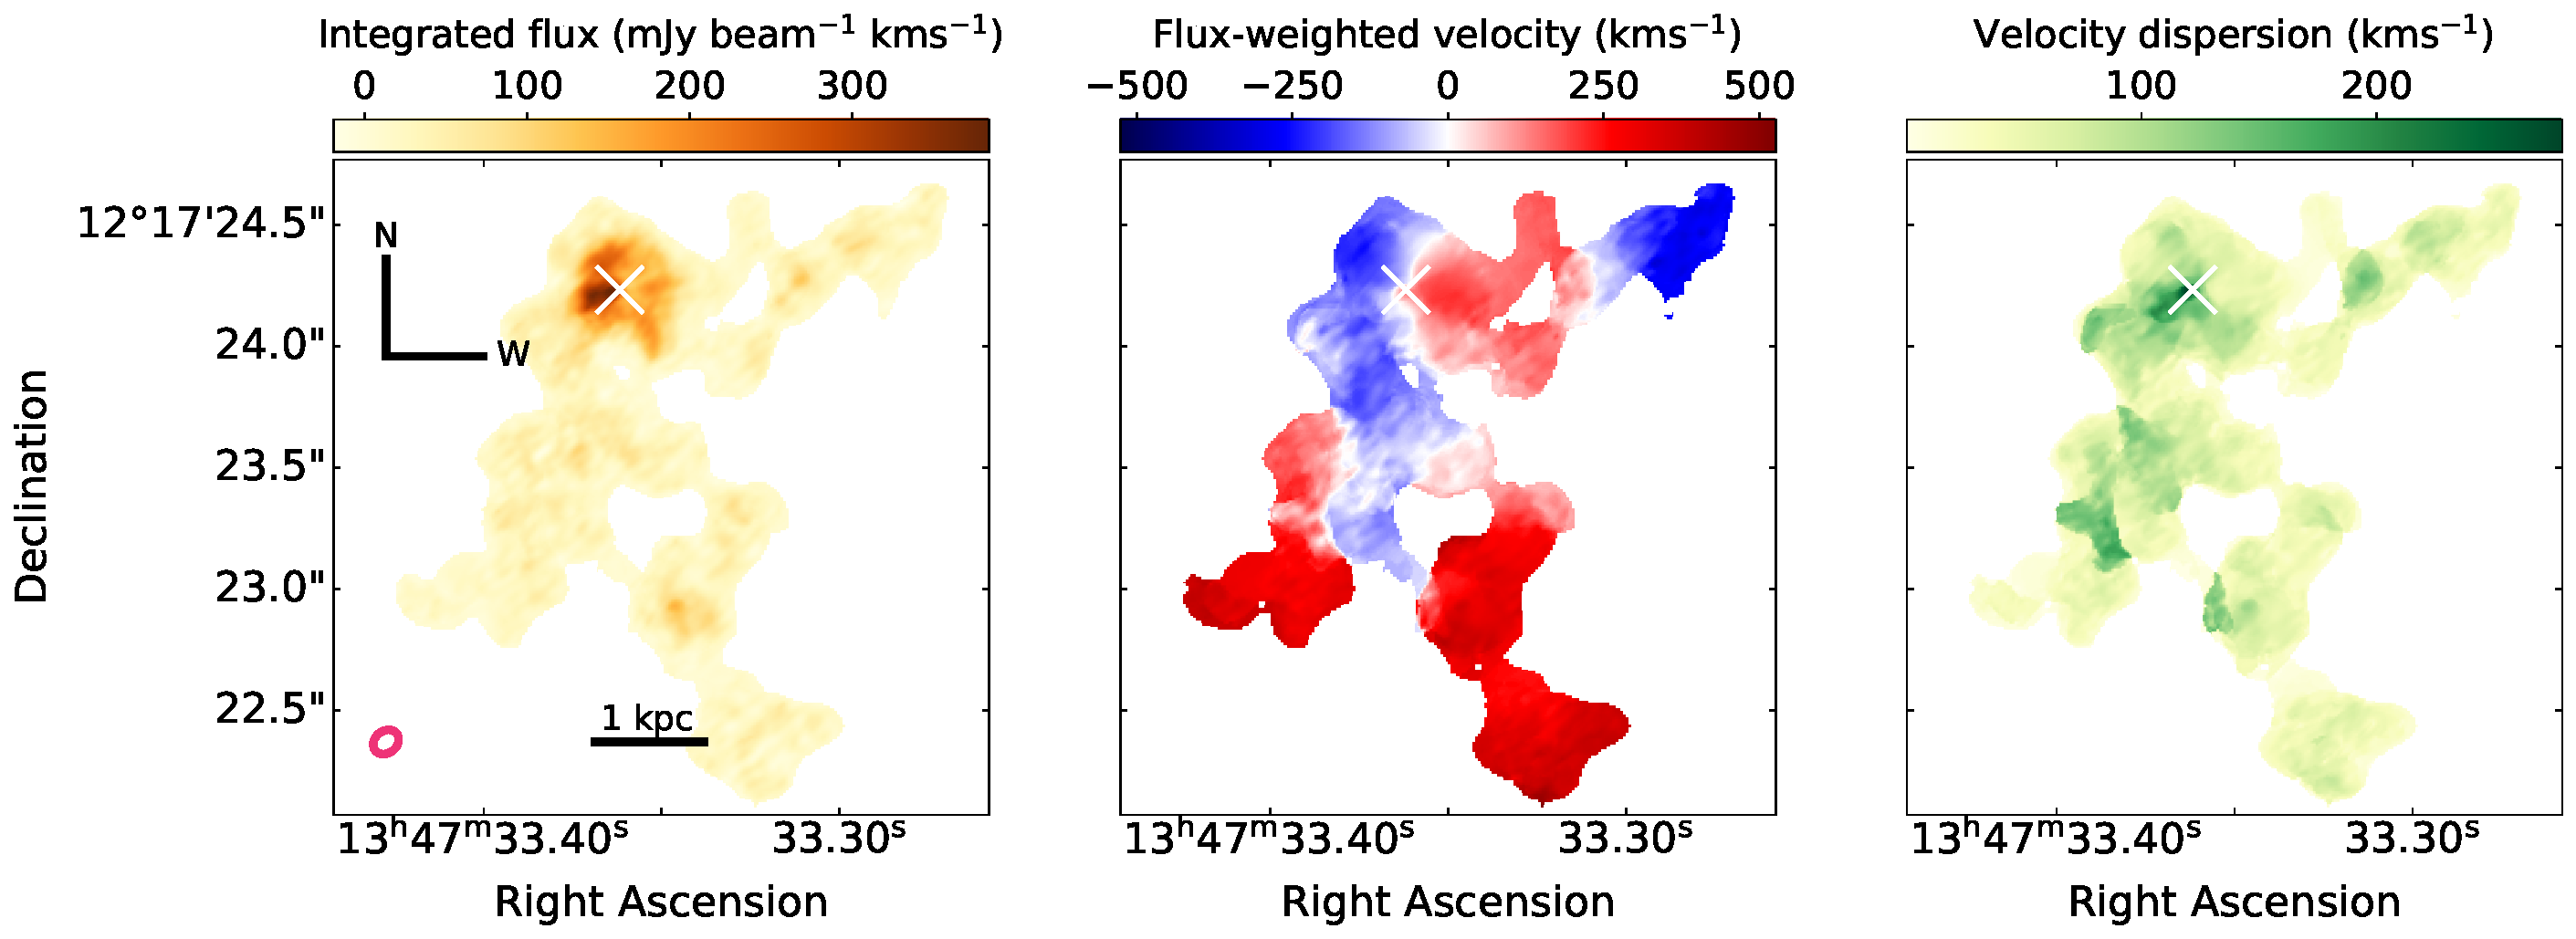
\includegraphics[width=1\linewidth, trim={0 1.5cm 0 0}, clip]{figures/alma_f13451_1232/large_fov_moment_maps.pdf}
    \end{subfigure} \\
    \vspace*{\baselineskip}
    \begin{subfigure}[]{\linewidth}
        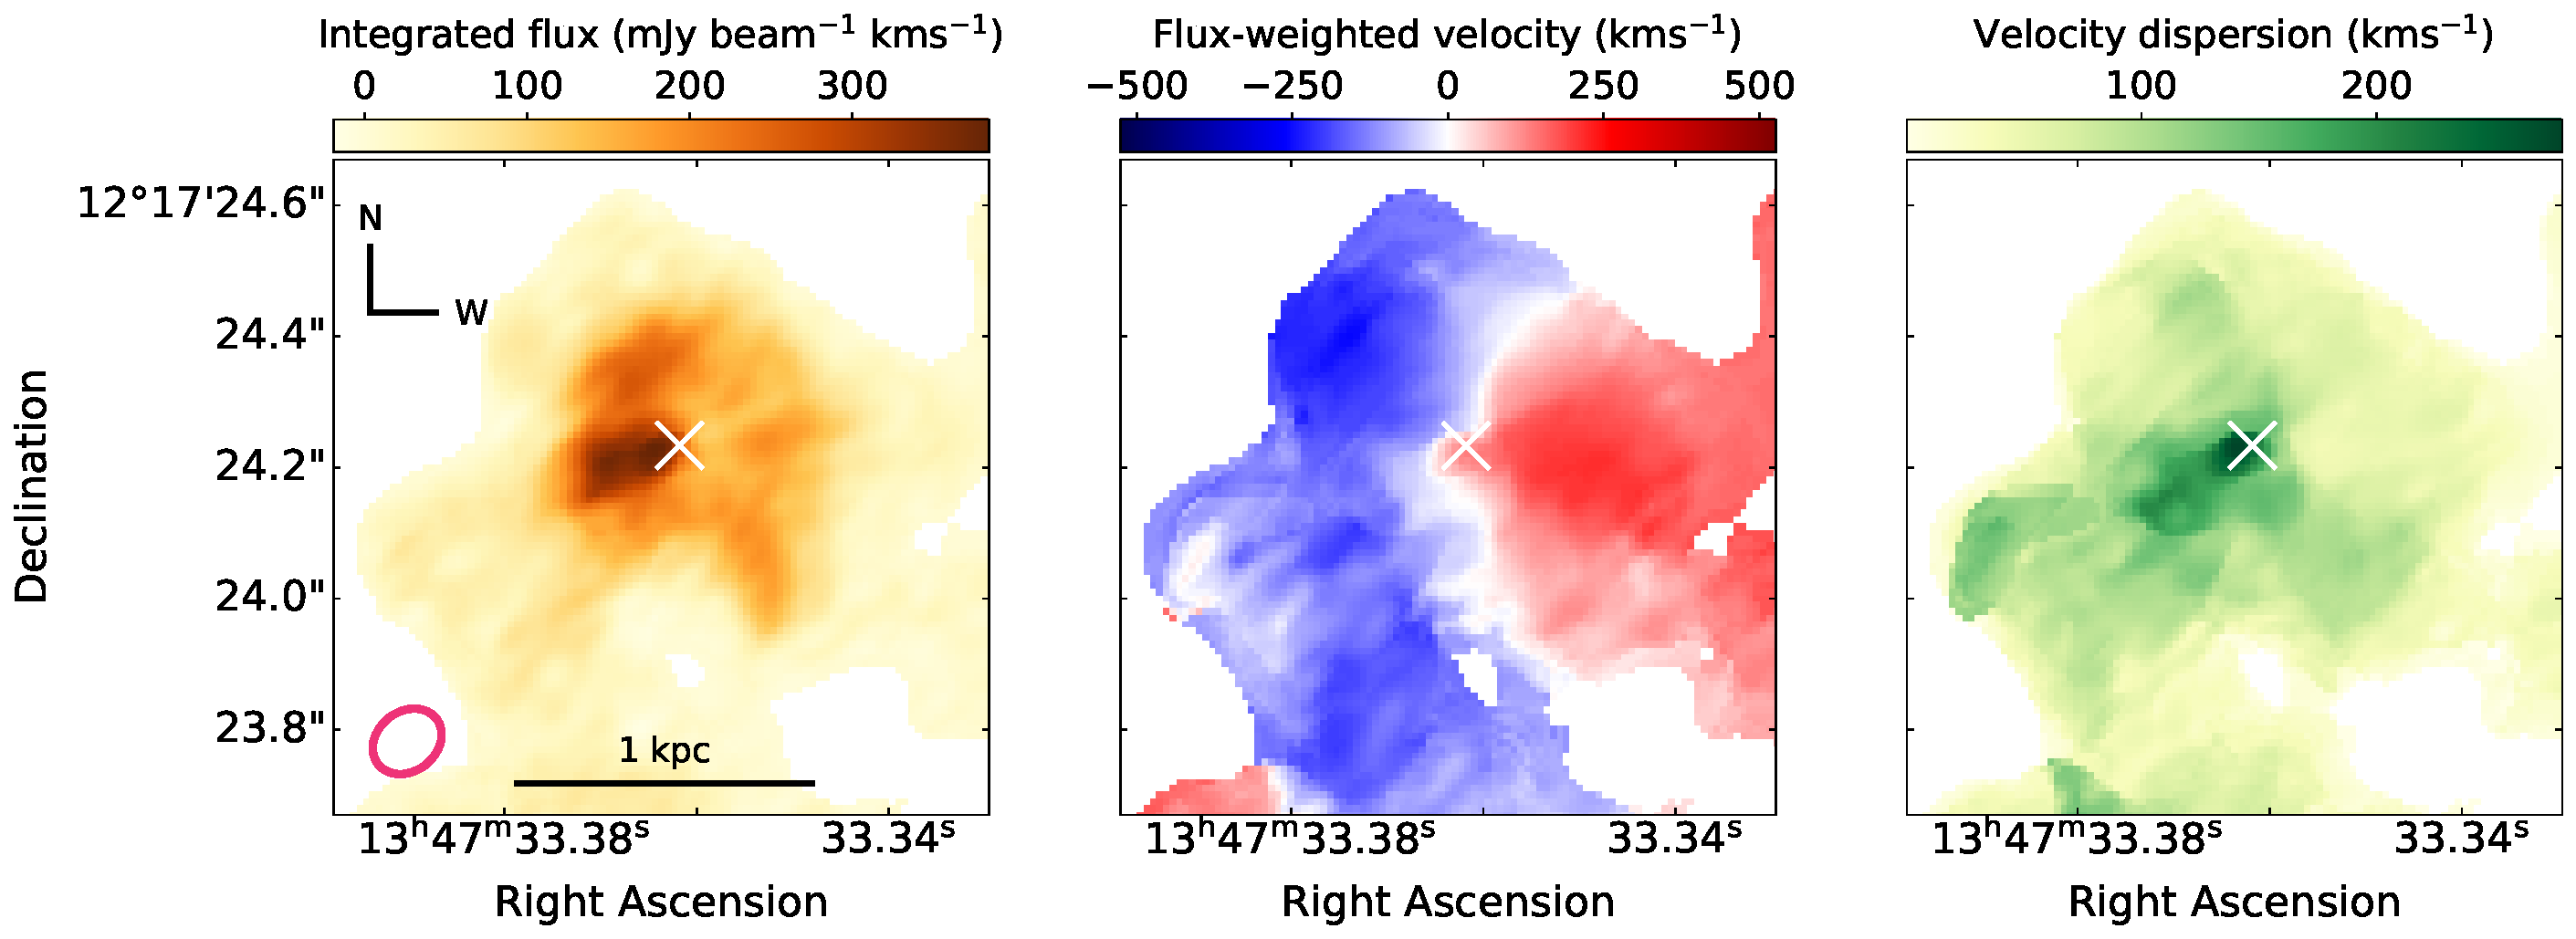
\includegraphics[width=1\linewidth, trim={0 0 0 2.93cm}, clip]{figures/alma_f13451_1232/moment_maps.pdf}
    \end{subfigure}
    \caption[Moment 0, 1, and 2 maps for the central kiloparsecs of the primary nucleus of F13451+1232.]{Integrated flux (moment 0; left panels), flux-weighted velocity (moment 1; middle panels), and velocity dispersion (moment 2; right panels) maps for the central $6\times6$\;kiloparsec (top panels) and inner-kiloparsec region (bottom panels) of the primary nucleus of F13451+1232. The white cross marks the continuum centre, which is taken to be the position of the AGN nucleus. The beam size of the observations is shown as a pink ellipse in the bottom left corner, and a 1\;kpc scale bar is shown in black.}
    \label{fig: alma_f13451_1232: moment_maps}
\end{figure*}

To investigate the flux and kinematic structures of the CO(1--0) emission around the primary nucleus of F13451+1232, moment maps of the combined datacube were created using the \textsc{SoFiA-2} source-finding pipeline \citep{Serra2015, Serra2021}. \textbf{In order to ensure that only genuine emission over a range of spatial scales (and of varying surface brightness) was included when producing the moment maps}, \textsc{SoFiA-2} first applied different combinations of spatial and velocity smoothing to the datacube: Gaussian filters with FWHMs of 0, 3, 6, 12, and 15 pixels were used for the spatial smoothing, and boxcar filters of widths 0, 3, 7, and 15 channels were used for the velocity smoothing. For each combination of spatial and velocity smoothing, emission above $4\sigma_\mathrm{rms}$ \textbf{(measured from the original cube in a region that did not contain emission)} was added to a total mask. This mask was then applied to the original, non-smoothed datacube, from which the maps in Figure\;\ref{fig: alma_f13451_1232: moment_maps} were produced. 

In the $6\times6$\;kpc moment maps (upper panels of Figure\;\ref{fig: alma_f13451_1232: moment_maps}), cold-molecular gas is detected to radial distances of $\sim$2.5\;arcseconds ($\sim$5.5\;kpc) south of the primary nucleus, and $\sim$1\;arcsecond ($\sim$2\;kpc) to the west. This large-scale ($r$\;\textgreater\;1\;kpc) emission, which has velocities in redshift and blueshift of up to $|v|\sim500$\;km\;s$^{-1}$, is indicative of gas that has been disturbed by the merger.

Within the central kiloparsec of the primary nucleus (Figure\;\ref{fig: alma_f13451_1232: moment_maps}), there is clear evidence for a disk with radius $r_\mathrm{disk}\sim0.5$\;kpc centred on the nucleus, blueshifted to the east and redshifted to the west, with a projected maximum flux-weighted velocity of 200--250\;km\;s$^{-1}$. In addition, there is an extended region (up to $r\sim0.3$\;arcseconds or 660\;pc from the nucleus along $\mathrm{PA}=120^\circ$) of emission with higher velocity dispersions ($\sigma$\;\textgreater\;150\;km\;s$^{-1}$) than that of the disk. Furthermore, a particularly prominent redshifted component with a velocity dispersion of $\sim$250\;km\;s$^{-1}$ is seen within a radius of $r\sim0.1$\;arcseconds ($r\sim220$\;pc) of the continuum centre.


\subsection{BBarolo modelling of the gas disk}
\label{section: alma_f13451_1232: analysis_and_results: disk}


To separate non-gravitational kinematics from those expected from a rotating gas disk, the disk was modelled using the \textsc{3DFIT} task from the \textsc{BBarolo} tool \citep{DiTeodoro2015}. The \textsc{3DFIT} task fits a series of concentric rings to the data in three spatial dimensions and three velocity dimensions (the rotational velocity, $v_\mathrm{rot}$; the radial velocity, $v_\mathrm{rad}$, and the velocity dispersion $v_\mathrm{disp}$).

The fitting procedure followed the methodology outlined in \citet{AlonsoHerrero2018}, \citet{DominguezFernandez2020}, and \citet{RamosAlmeida2022}. Throughout, the centre of the disk model was fixed to be the position of the continuum centre (as measured from a two-dimensional Gaussian fit to the continuum image: Section\;\ref{section: alma_f13451_1232: observations_and_data_reduction}). An initial fit was first performed using the \textsc{3DFIT} task in which the radial velocities of the rings were fixed to be 0\;km\;s$^{-1}$ and the scale height of the disk ($z_\mathrm{0}$) was fixed to 0\;pc. The remaining parameters were allowed to vary; initial values for the rotational velocity and velocity dispersion were based on the flux-weighted velocity shift and velocity dispersion maps (Figure\;\ref{fig: alma_f13451_1232: moment_maps}), the initial value of the inclination ($i_\mathrm{initial}=38^\circ$) was based on the measured ratio of the projected disk major and minor axes while assuming a circular disk, and the initial value for the PA was set to that previously estimated from two-dimensional spectroastrometry of CO(2--1) observations of the disk by \citet{Lamperti2022}. However, limits were imposed on the variation of these free parameters --- between successive rings, the rotational velocity was not allowed to change by more than $\pm$50\;km\;s$^{-1}$, nor were the inclination and PA allowed to change by more than $\pm20^\circ$. The fits used uniform weighting and local normalisation. It should be noted that, since the physical size of the modelled rings is much less than the beam size of the observations, the properties of adjacent rings are correlated. However, this does not have a significant effect on the maximum rotational velocity of the disk model (nor does changing the values of the initial parameters), and therefore does not affect the interpretations made in this analysis.

\begin{figure*}[!p]
    \centering
    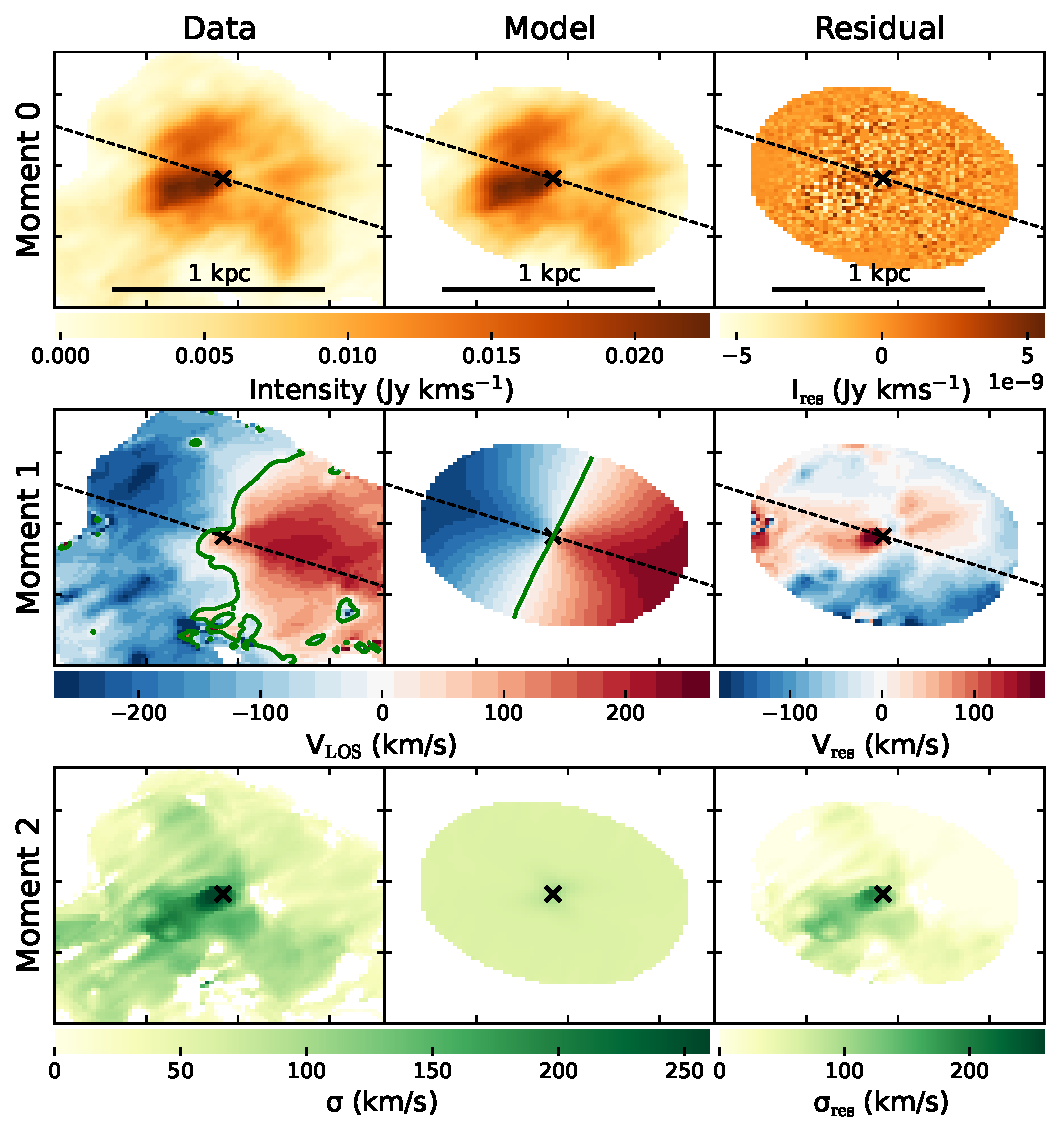
\includegraphics[width=\linewidth]{figures/alma_f13451_1232/disk_moment_maps.pdf}
    \caption[Moment 0, 1, and 2 maps (and residuals = data - model) for the \textsc{BBarolo 3DFit} model of the kiloparsec-scale disk in the primary nucleus of F13451+1232.]{Integrated flux (moment 0; top), flux-weighted velocity (moment 1; middle), and velocity dispersion (moment 2; bottom) maps of the CO(1--0) data (left), the \textsc{BBarolo} disk model (middle), and residuals (data - model; right). The ticks have separations of 0.2\;arcseconds. The black dashed line shows the PA of the modelled disk, whereas the black cross shows the disk centre (which was set to be the continuum centre position; see Section\;\ref{section: alma_f13451_1232: observations_and_data_reduction}). The green lines in the middle-row panels are isovelocity contours at 0\;km\;s$^{-1}$.}
    \label{fig: alma_f13451_1232: bbarolo_model}
\end{figure*}


In order to ensure that the overall radial extent and kinematics of the disk were accurate --- and to alleviate potential problems with fit degeneracy arising from having a high number of free parameters --- the results of the initial fit were used as a basis for a second fit. For this second run, I fixed the velocity dispersion, inclination, and PA to the values determined from the first run, so that only the rotational velocity was allowed to vary. The final model parameters for each ring are presented in Table\;\ref{tab: bbarolo_model}; Figure\;\ref{fig: alma_f13451_1232: bbarolo_model} presents the moment maps and residuals of the final disk model. High flux-weighted velocities ($V_\mathrm{LOS}$\;\textgreater\;200\;km\;s$^{-1}$) and velocity dispersions ($\sigma\sim200$\;km\;s$^{-1}$) due to non-rotational kinematics can be seen in the residual maps near the centre of the disk.

In the final \textsc{BBarolo} model, the disk has an average inclination of $i\approx54^\circ$ (where $i=0^\circ$ corresponds to the disk being face-on), and its major axis lies along $\mathrm{PA}\approx248^\circ$; the deprojected rotational velocity increases from $v_\mathrm{rot}=246$\;km\;s$^{-1}$ to $v_\mathrm{rot}=307$\;km\;s$^{-1}$ over the radius range 28\;pc\;\textless\;$r_\mathrm{disk}$\;\textless\;560\;pc. I highlight that the purpose of this modelling was solely to give a reasonable estimate of the maximum rotational velocity of the molecular gas, which is needed to robustly identify non-rotational motions. Considering this, it is notable that the high-velocity-dispersion emission ($\sigma$\;\textgreater\;150\;km\;s$^{-1}$) seen near the disk in the moment maps (Figure\;\ref{fig: alma_f13451_1232: moment_maps}) cannot be accounted for by the \textsc{BBarolo} model (see Figure\;\ref{fig: alma_f13451_1232: bbarolo_model}), and thus cannot be explained as being part of the rotating gas disk. 


\begin{table*}[!t]
    \centering
    \renewcommand{\arraystretch}{1.2}
    \begin{tabular}{cccccc}
    $r_\mathrm{ring}$\;(arcseconds) & $r_\mathrm{ring}$\;(pc) & $v_\mathrm{rot}$\;(km\;s$^{-1}$) & $v_\mathrm{disp}$\;(km\;s$^{-1}$) & $i$\;$(^\circ)$  & PA\;$(^\circ)$ \\ \hline
    0.013     & 29    & 248    & 5.5      & 62.2   & 242   \\
    0.040     & 88    & 250    & 24.6     & 58.6   & 236   \\
    0.067     & 147    & 212    & 91.1     & 55.9   & 236   \\
    0.094     & 206    & 249    & 72.5     & 53.8   & 240   \\
    0.121     & 265    & 268    & 65.8     & 52.4   & 245   \\
    0.148     & 324    & 281    & 62.8     & 51.4   & 252   \\
    0.175     & 383    & 293    & 61.2     & 50.8   & 258   \\
    0.202     & 442    & 312    & 68.3     & 50.5   & 261   \\
    0.229     & 501    & 301    & 61.5     & 50.3   & 259   \\
    0.256     & 560    & 314    & 58.3     & 50.1   & 252  
    \end{tabular}
    \caption[Parameters of the \textsc{BBarolo 3DFit} model of the kiloparsec-scale disk in the primary nucleus of F13451+1232.]{Final parameters for each ring of the \textsc{BBarolo 3DFit} disk model. The distance of each ring to the fixed disk centre ($r_\mathrm{ring}$) is given in both arcseconds and parsecs. Here, $v_\mathrm{rot}$ and $v_\mathrm{disp}$ are the rotational velocities and velocity dispersions of each ring, respectively.}
    \label{tab: bbarolo_model}
\end{table*}


\subsection{Kinematics of the non-rotating gas}
\label{section: alma_f13451_1232: analysis_and_results: outflow_kinematics}

To investigate the non-rotational kinematics further, I binned the velocity channels of the original cube by a factor of three and applied Hanning smoothing using the \textsc{CASA} software suite \citep{Bean2022} to improve the signal-to-noise ratio of the emission. This resulted in a cube of velocity resolution 86.4\;km\;s$^{-1}$ and an RMS noise of $0.083$\;mJy\;beam$^{-1}$. Using the \textsc{pvextractor Python} module\footnote{\url{https://pvextractor.readthedocs.io/en/latest/}}, $1.00\times0.05$\;arcsecond slices, centred on the nucleus, were extracted from both this datacube and the \textsc{BBarolo} disk-model datacube along the major axis of the disk ($\mathrm{PA}=248^\circ$) and in the direction of the high-velocity-dispersion gas near the nucleus ($\mathrm{PA}=120^\circ$). From these slices, position-velocity (PV) diagrams were produced, which are presented in Figure\;\ref{fig: alma_f13451_1232: pv_diagrams}. In the PV diagrams, there is clear evidence for non-rotational kinematics, with detected velocities being well above the projected maximum rotational disk velocity given by the \textsc{BBarolo} model. There is intermediate-velocity emission (300\;\textless\;$|v|$\;\textless\;400\;km\;s$^{-1}$) seen in both blueshift and redshift along $\mathrm{PA}=120^\circ$, in the ranges 0.1\;\textless\;$r$\;\textless\;0.3\;arcseconds and 0.0\;\textless\;$r$\;\textless\;0.2\;arcseconds, respectively, to the southeast (SE) of the nucleus. Moreover, the compact ($r$\;\textless\;0.1\;arcseconds) redshifted feature visible in the moment maps (Figure\;\ref{fig: alma_f13451_1232: moment_maps}) can be seen in the PV diagrams between 400\;\textless\;$v$\;\textless\;680\;km\;s$^{-1}$, located close to the nucleus.

\begin{figure*}[!p]
    \centering
    \begin{subfigure}[b]{0.75\textwidth}
        \centering
        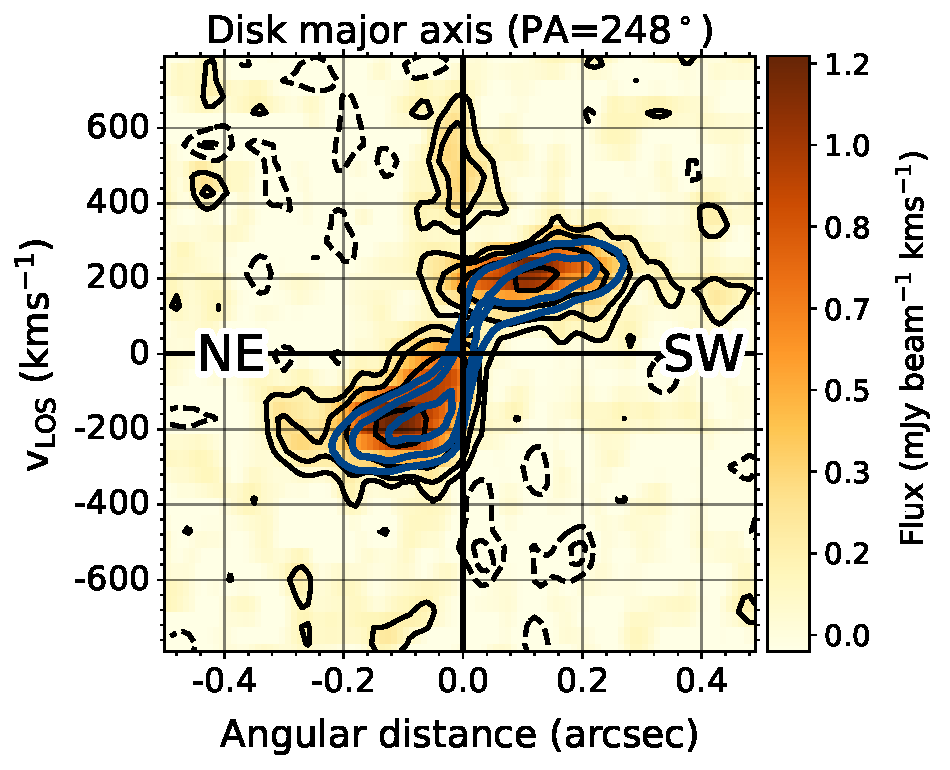
\includegraphics[width=\textwidth]{figures/alma_f13451_1232/pv_248deg.pdf}
    \end{subfigure}
    \hspace{1em}
    \begin{subfigure}[b]{0.75\textwidth}
        \centering
        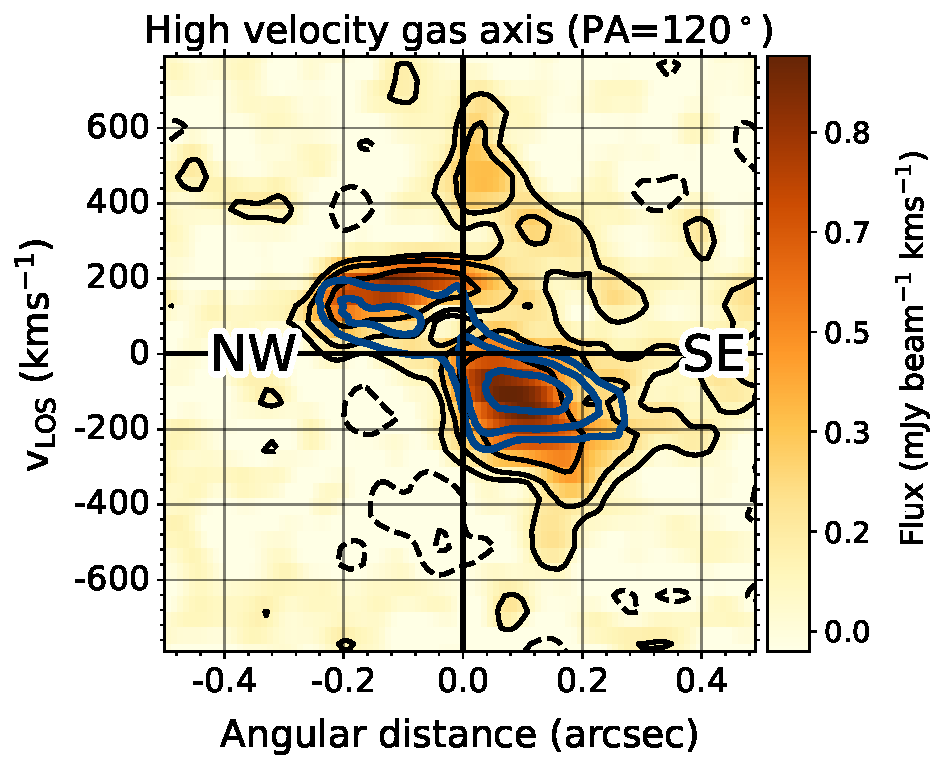
\includegraphics[width=\textwidth]{figures/alma_f13451_1232/pv_120deg.pdf}
    \end{subfigure}
    \caption[CO(1--0) position-velocity (PV) diagrams for $1.00\times0.05$\;arcsecond slices with $\mathrm{PA}=248^\circ$ and $\mathrm{PA}=120^\circ$, centred on the primary nucleus of F13451+1232.]{Position-velocity (PV) diagrams for $1.00\times0.05$\;arcsecond slices with $\mathrm{PA}=248^\circ$ (upper panel; the major axis of the disk) and $\mathrm{PA}=120^\circ$ (lower panel; the direction of the high-velocity-dispersion emission seen in Figure\;\ref{fig: alma_f13451_1232: moment_maps}), centred on the continuum centre. CO(1--0) emission is shown in yellow/orange, with black contours at the $-3\sigma_\mathrm{rms}$, $-1.5\sigma_\mathrm{rms}$, 1.5$\sigma_\mathrm{rms}$, 3$\sigma_\mathrm{rms}$, 6$\sigma_\mathrm{rms}$, and 12$\sigma_\mathrm{rms}$ levels (dashed: negative; solid: positive); solid blue contours show the flux from the \textsc{BBarolo} disk model at the same $\sigma_\mathrm{rms}$ levels. Extended, intermediate-velocity emission is seen in both redshift and blueshift in the $\mathrm{PA}=120^\circ$ diagram, and a compact, higher-velocity feature (400\;\textless\;$v$\;\textless\;680\;km\;s$^{-1}$) centred approximately on the nucleus (0.0\;arcsec) can clearly be seen in both diagrams.}
    \label{fig: alma_f13451_1232: pv_diagrams}
\end{figure*}

\begin{figure}[!h]
    \centering
    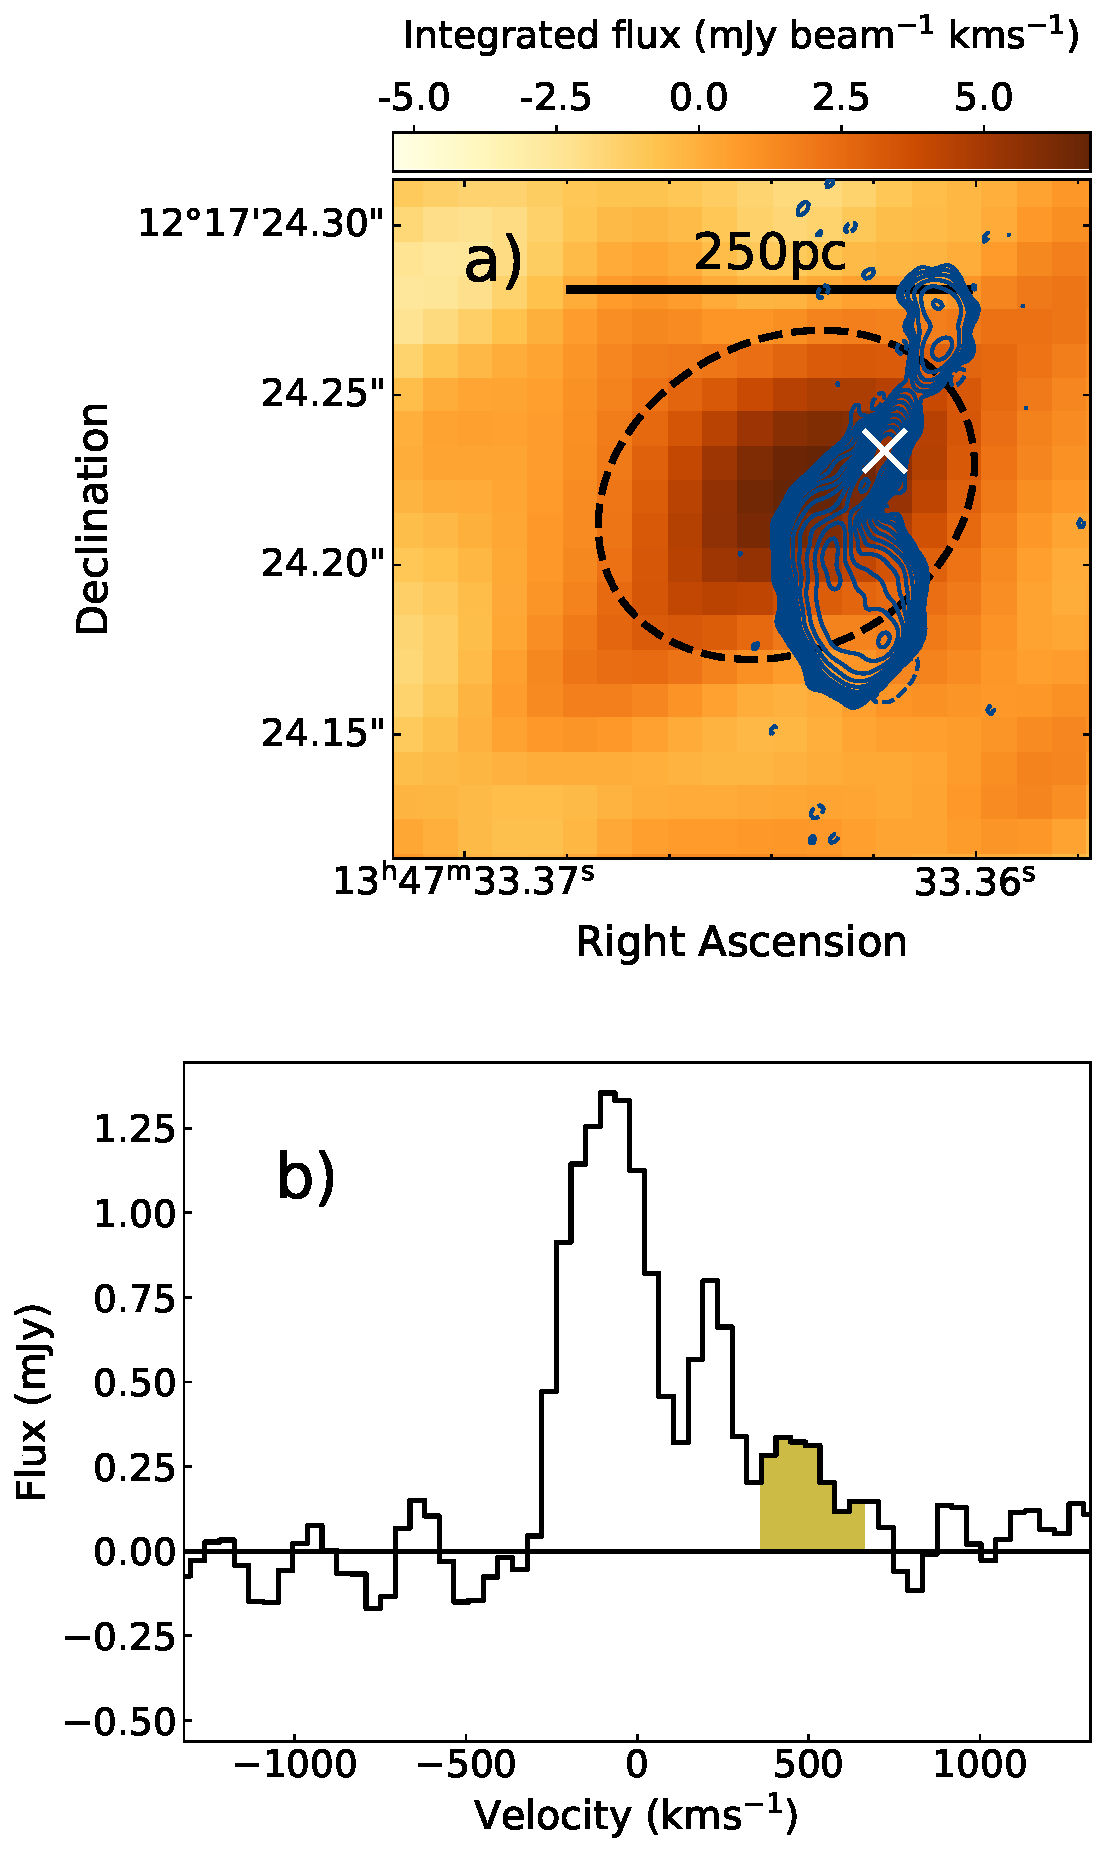
\includegraphics[width=0.65\linewidth]{figures/alma_f13451_1232/outflow_moment_map.pdf}
    \caption[\textbf{a)} Integrated CO(1--0) flux map of the nuclear outflow in F13451+1232, with VLBI 1266\;MHz continuum imaging from \citet{Morganti2013_4c1250} showing the small-scale radio structure; \textbf{b)} CO(1--0) velocity profile of the nuclear outflow.]{\textbf{a)} Integrated flux map (orange--brown) of the velocity channels between 400\;\textless\;$v$\;\textless\;680\;km\;s$^{-1}$. The dashed black ellipse shows the aperture extracted from the datacube to derive the mass of the outflow; the corresponding line profile is shown in Figure\;\ref{fig: alma_f13451_1232: outflow_moment_map}b. The small-scale radio structure, as seen in VLBI 1266\;MHz continuum imaging \citep{Morganti2013_4c1250}, is shown as dark blue solid contours at the $0.3\times$($-1$, 1, 2, 4, 8, 16, 32, 64, 128, 256, 512, 1024) mJy/beam levels, whereas the white cross marks the position of the continuum centre seen in the ALMA CO(1--0) observations (Section\;\ref{section: alma_f13451_1232: observations_and_data_reduction}). \textbf{b)}\;CO(1--0) line profile extracted from the aperture that covers the outflow; the line profile shown was extracted from the 84\;km\;s$^{-1}$ velocity resolution combined datacube. The part of the line profile that is taken to represent outflowing gas (400\;\textless\;$v$\;\textless\;680\;km\;s$^{-1}$) is shaded in yellow.}
    \label{fig: alma_f13451_1232: outflow_moment_map}
\end{figure}

\subsection{Comparison to the small-scale radio structure}
\label{section: alma_f13451_1232: analysis_and_results: radio_structure}

Due to the velocities at which the compact, high-velocity nuclear feature is detected, it is unambiguously distinct from the rotating gas disk: it may be interpreted as either an inflow moving towards the nucleus on the observer's side of the disk, or an outflow originating from the nucleus on the far side of the disk. Spatial comparison of the high-velocity flow to the small-scale radio structure may provide an indication of the nature of this flowing gas and, if it is an outflow, the driving mechanism. Figure\;\ref{fig: alma_f13451_1232: outflow_moment_map}a shows the flux map integrated over the range 400\;\textless\;$v$\;\textless\;680\;km\;s$^{-1}$ --- in which peak emission is detected above the 6$\sigma_\mathrm{rms}$ level --- along with VLBI 1266\;MHz continuum imaging (from global VLBI experiment GM62B; data presented and detailed in \citealt{Morganti2013_4c1250}) of the central $0.20\times0.20$\;arcseconds ($440\times440$\;parsecs). The beam size of the VLBI observations was $8.01\times4.89$\;milliarcseconds ($\mathrm{PA}=-20.2^\circ$). Due to the small uncertainties in the ALMA pointing, the VLBI image was offset from the continuum centre by $\sim$0.1\;arcseconds; this pointing error was corrected for by aligning the compact core seen in the VLBI image with the continuum centre, as it is expected that the same source is being imaged at different spatial resolutions. 

By fitting a two-dimensional Gaussian profile to the integrated high-velocity CO(1--0) emission in Figure\;\ref{fig: alma_f13451_1232: outflow_moment_map}a using the \textsc{emcee} Python module \citep{FormanMackey2013}, it was found to be offset to the southeast (SE) of the continuum centroid by \textbf{$32\pm2$\;milliarcseconds} ($70\pm4$\;pc) along $\mathrm{PA}\sim155^{\circ}$. I highlight that this is within the spatial extent of, and has a similar PA to, the small-scale radio structure ($r\sim0.07$\;arcsec; $\mathrm{PA}=151^\circ$).


\subsection{Channel maps}
\label{section: alma_f13451_1232: analysis_and_results: channel_maps}

To determine the level at which the high-velocity, nuclear \mbox{CO(1--0)} emission is detected in different velocity channels, I created channel maps of the central kiloparsec of the primary nucleus from the 86.4\;km\;s$^{-1}$ velocity resolution cube. The high-velocity (400\;\textless\;$v$\;\textless\;600\;km\;s$^{-1}$) channel maps --- presented in Figure\;\ref{fig: alma_f13451_1232: channel_maps} --- show emission above the 3$\sigma_\mathrm{rms}$ level (and up to 4$\sigma_\mathrm{rms}$) in all four channels on scales similar to that of the beam size (0.11\;arcseconds or 240\;pc), indicating that the feature is spatially-unresolved in the combined datacube. 

\begin{figure}[!b]
    \centering
    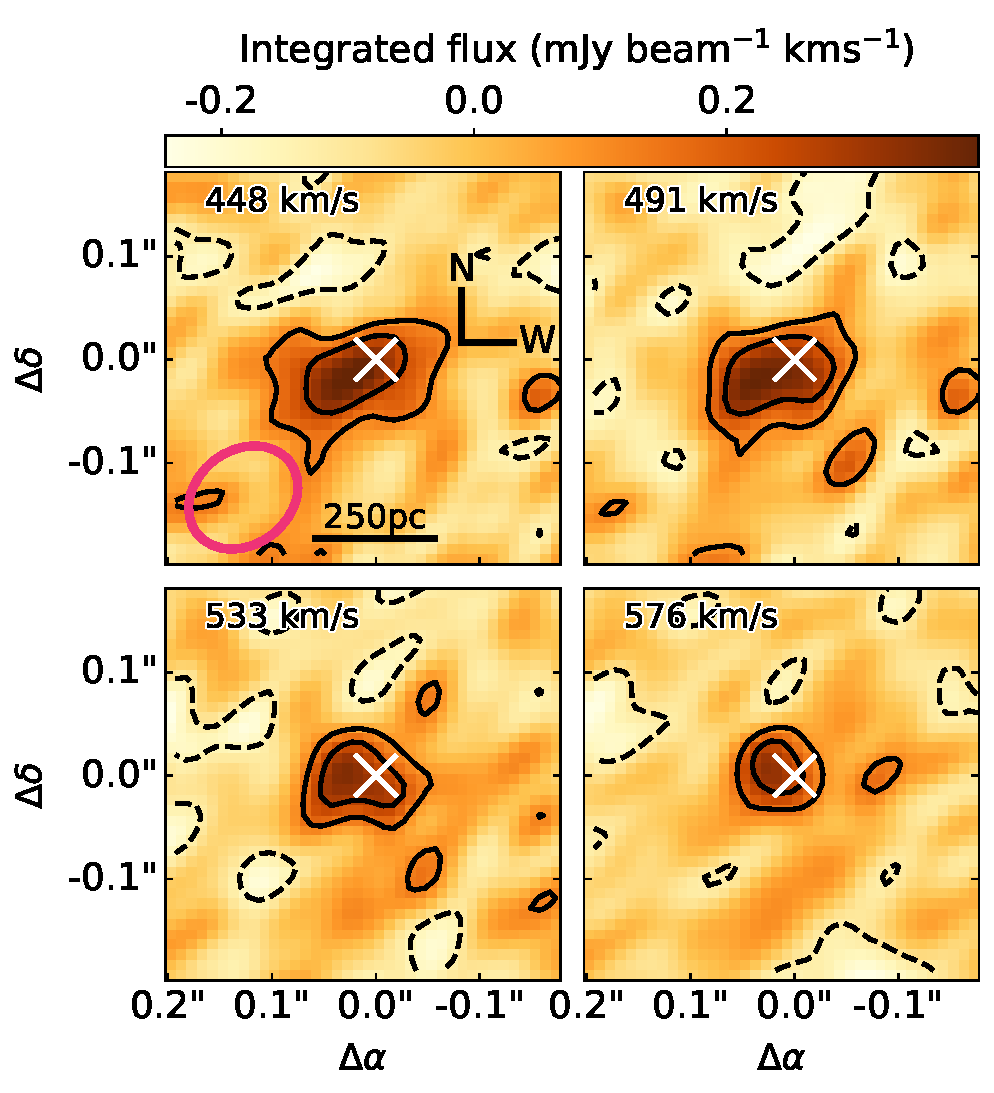
\includegraphics[width=0.66\linewidth]{figures/alma_f13451_1232/channel_maps.pdf}
    \caption[Velocity channel maps of the central $\sim$1\;kpc of the primary nucleus of F13451+1232.]{Channel maps of the central $\sim$1\;kpc of the primary nucleus of F13451+1232 (centred on the nucleus: Section\;\ref{section: alma_f13451_1232: observations_and_data_reduction}) between 448\;\textless\;$v$\;\textless\;576\;km\;s$^{-1}$, taken from the velocity-binned and smoothed cube with channel widths of 43.7\;km\;s$^{-1}$ and a velocity resolution of 86.4\;km\;s$^{-1}$. Black contours are shown at the $-3\sigma_\mathrm{rms}$, $-1.5\sigma_\mathrm{rms}$, 1.5$\sigma_\mathrm{rms}$, 3$\sigma_\mathrm{rms}$ levels (dashed: negative; solid: positive), where $\sigma_\mathrm{rms}$ is the RMS of the binned-and-smoothed cube. The continuum centre is marked as a white cross in each channel; the beam size is shown as a pink ellipse in the 448\;km\;s$^{-1}$ channel map (top left panel).}
    \label{fig: alma_f13451_1232: channel_maps}
\end{figure}

\subsection{Potential effects of continuum subtraction}
\label{section: alma_f13451_1232: analysis_and_results: potential_effects_of_continuum_subtraction}

Due to the bright, steep-spectrum continuum around the CO(1--0) line --- originating from primary nucleus of F13451+1232 (as seen in the cores of other CSS/GPS sources, e.g. \citealt{Oosterloo2019}) --- it is possible that inaccuracies in the continuum subtraction process have contributed flux to the compact, redshifted, high-velocity feature that is detected at the position of the nucleus. However, I argue that this feature represents real CO(1--0) emission, for several reasons. Firstly, the flux is detected above the $6\sigma$ level in the flux map integrated over the velocity range 400\;\textless\;$v$\;\textless\;680\;km\;s$^{-1}$ (Figure\;\ref{fig: alma_f13451_1232: outflow_moment_map}a), and in multiple velocity channels at the 3--4$\sigma_\mathrm{rms}$ levels (Figure\;\ref{fig: alma_f13451_1232: channel_maps}). Secondly, it has a significantly higher flux than the negative or positive residual features detected in the integrated spectrum (Figure\;\ref{fig: alma_f13451_1232: outflow_moment_map}b). 

Moreover, in Figure\;\ref{fig: alma_f13451_1232: beam_comparison}, I present CO(1--0) line spectra extracted from the two cubes of differing spatial resolution that comprise the combined datacube (Section\;\ref{section: alma_f13451_1232: observations_and_data_reduction}); the size of the extraction aperture in each case was matched to the beam size. The high-velocity redshifted feature is well detected in both datacubes in the velocity range 400\;\textless\;$v$\;\textless\;680\;km\;s$^{-1}$, while any residual features of comparable flux are not present in both cubes at the same velocity. Furthermore, its absolute flux is less in the smaller-beam cube, indicating that the beam is not recovering all of the flux and thus implying that the feature is (partially) spatially resolved. While some contribution from instrumental effects cannot be entirely ruled out, based on these arguments, I conclude that this feature is real.


\begin{figure}[!b]
    \centering
    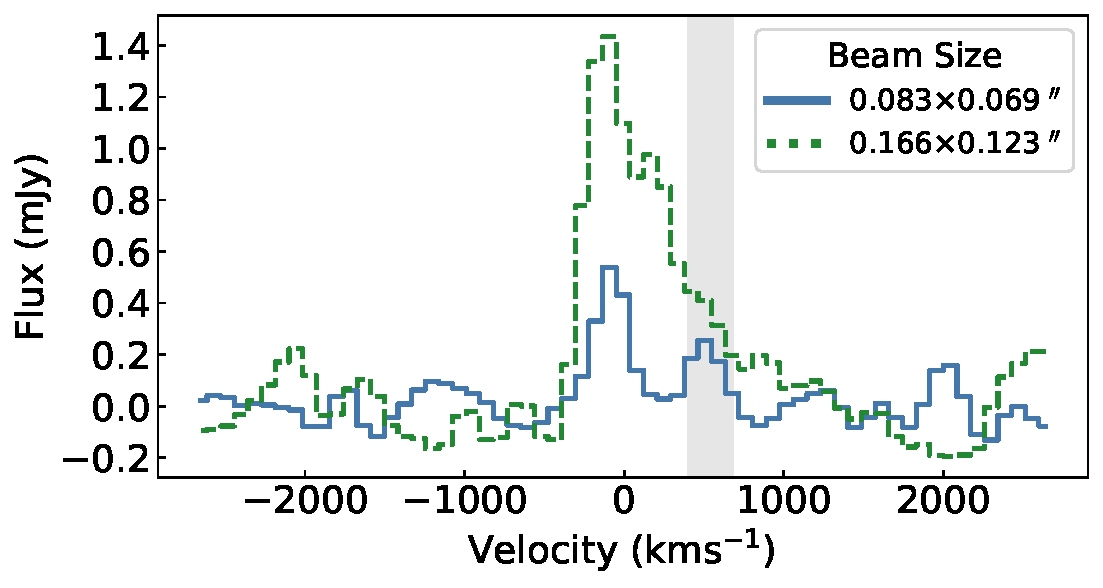
\includegraphics[width=0.75\linewidth]{figures/alma_f13451_1232/beam_comparison.pdf}
    \caption[CO(1--0) velocity profiles of the nuclear outflow in the primary nucleus of F13451+1232 extracted from observations of differing array configurations (hence beam sizes).]{CO(1--0) line profiles of the primary nucleus of F13451+1232 extracted from the two sets of observations of differing array configurations (hence beam sizes) that comprise the datacube presented in this analysis (see Section\;\ref{section: alma_f13451_1232: observations_and_data_reduction}). These profiles were extracted from the respective cubes using apertures matched to the beam sizes. It can be seen that the flux in the high-velocity redshifted component (shaded in grey) is less in the cube with the smaller beam size.}
    \label{fig: alma_f13451_1232: beam_comparison}
\end{figure}

It is notable that previous CO(2--1) observations of the primary nucleus of F13451+1232 --- that were of similar sensitivity to the CO(1--0) observations presented here --- did not detect evidence for nuclear outflows \citep{Lamperti2022}. However, in those observations, the other spectral windows were also used when fitting a linear slope to the continuum because of the narrower observing band (a factor of two narrower in velocity) of CO(2--1) observations relative to CO(1--0) --- this may have led to over-subtraction of the high-velocity outflow component. Therefore, it is possible that outflow emission in CO(2--1) was not detected due to uncertainties in the continuum subtraction process.

\subsection{Outflow energetics}
\label{section: alma_f13451_1232: analysis_and_results: outflow_energetics}

In order to provide an estimate of the mass inflow/outflow rates of the high-velocity, spatially-unresolved redshifted feature located at the position of the nucleus, an elliptical aperture matching the beam size ($0.113\times0.091$\;arcsec, PA$=-51.8^\circ$; shown in Figure\;\ref{fig: alma_f13451_1232: outflow_moment_map}a) was extracted from the datacube. I then summed all pixels within the aperture to create a line profile, which is presented in Figure\;\ref{fig: alma_f13451_1232: outflow_moment_map}b, and selected emission between 400\;\textless\;$v$\;\textless\;680\;km\;s$^{-1}$ to isolate the non-rotating gas. 

For the extended, intermediate-velocity (300\;\textless\;$|v|$\;\textless\;400\;km\;s$^{-1}$) emission seen in blueshift and redshift, two sub-apertures were extracted from the $1.00\times0.05$\;arcsecond slice along $\mathrm{PA}=120^\circ$ (used to create the upper PV diagram in Figure\;\ref{fig: alma_f13451_1232: pv_diagrams}): one covering radii 0.0\;\textless\;$r$\;\textless\;0.2\;arcseconds (for the extended redshifted emission), and the other covering the range 0.1\;\textless\;$r$\;\textless\;0.3\;arcseconds (for the extended blueshifted emission). I then selected emission in the ranges 300\;\textless\;$v$\;\textless\;400\;km\;s$^{-1}$ and $-400$\;\textless\;$v$\;\textless$-300$\;km\;s$^{-1}$ respectively in these slices to isolate the non-rotating gas.

For every channel within the range of the selected velocities in the extracted apertures, CO(1--0) fluxes ($S_\mathrm{CO}\Delta V$) were calculated and converted to luminosities ($L^\prime_\mathrm{CO}$) using the relation presented by \citet{Solomon2005}:
\begin{equation}
    L^\prime_\mathrm{CO} = 3.25\times10^7 S_\mathrm{CO}\Delta V {\nu}^{-2}_\mathrm{obs}D^2_\mathrm{L}(1+z)^{-3},
    \label{eq: alma_f13451_1232: co_luminosity}
\end{equation}
where ${\nu}_\mathrm{obs}$ is the observed frequency of the CO(1--0) line (102.789\;GHz) and $D_\mathrm{L}$ is the luminosity distance to F13451+1232. The CO(1--0) luminosities were then summed across all selected velocity channels, resulting in total luminosities for each of the two intermediate-velocity features and the high-velocity feature. Assuming a CO-to-H$_\mathrm{2}$ conversion factor of $\alpha_\mathrm{CO}=0.8$\;M$_\odot$\;(K\;km\;s$^{-1}$\;pc$^2$)$^{-1}$ (typical for ULIRGs: \citealt{Downes1998}), these total luminosities were converted into molecular gas masses ($M_\mathrm{flow}$). 

By taking an aperture covering the disk in the combined CO(1--0) datacube and integrating between $-310$\;\textless\;$v$\;\textless\;$310$\;km\;s$^{-1}$, a disk mass of $1.1\times10^{10}$\;M$_\odot$ was found using Equation \ref{eq: alma_f13451_1232: co_luminosity} and $\alpha_\mathrm{CO}=0.8$\;M$_\odot$\;(K\;km\;s$^{-1}$\;pc$^2$)$^{-1}$; \citet{Lamperti2022} also detected this nuclear disk using CO(2-1) spectroastrometry, and found a similar mass.

The corresponding mass flow rates of the non-rotating molecular gas were estimated using
\begin{equation}
    \dot{M}_\mathrm{flow} = \frac{M_\mathrm{flow}v_w}{\Delta R} \cdot \mathrm{tan\theta},
\end{equation}
where $v_w$ is the flux-weighted velocity, $\Delta R$ is the range of flow radii, and $\theta$ is the angle of the flow relative to the observer's line of sight. The $\mathrm{tan\theta}$ term is required to correct for projection effects in both radius and velocity. To estimate this projection factor, I assumed a solid-angle-weighted mean inclination for random orientations of the line of sight to the flow direction, giving $\theta=57.3^\circ$ \textbf{(see \citealt{Law2009} for a full derivation)}. Finally, kinetic powers were estimated with
\begin{equation}
    \dot{E}_\mathrm{kin}=\frac{1}{2}\dot{M}_\mathrm{flow}\Bigl(\frac{v_w}{\mathrm{cos\theta}}\Bigl)^2.
    \label{eq: alma_f13451_1232: kinetic_power}
\end{equation}
The resulting CO(1--0) luminosities, masses, flux-weighted velocities, flow radii, mass flow rates, kinetic powers, and coupling efficiencies ($\epsilon_\mathrm{f}=\dot{E}_\mathrm{kin}$/$L_\mathrm{bol}$) are given in Table\;\ref{tab: outflow_properties}. For the high-velocity nuclear gas, I derived a mass flow rate of $\dot{M}_\mathrm{out}\sim230$\;M$_\odot$\;yr$^{-1}$, which corresponds to a kinetic power that is $\sim$1.4\;per\;cent of the bolometric luminosity of the AGN ($L_\mathrm{bol}=4.8\times10^{45}$\;erg\;s$^{-1}$: \citealt{Rose2018}). In contrast, much lower mass flow rates ($\dot{M}_\mathrm{out}=22$--$27$\;M$_\odot$\;yr$^{-1}$) and kinetic powers ((6.0--7.1)$\times10^{-2}$\;per\;cent of $L_\mathrm{bol}$) were found for the extended, intermediate-velocity emission.

\begin{table*}[!t]
    \centering
    \renewcommand{\arraystretch}{1.1}
    \begin{tabular}{lcccc}
        \multirow{2}{*}{Component} & $L^\prime_\mathrm{CO}$  & $M_\mathrm{flow}$  & $v_\mathrm{w}$  & ${\Delta}R$ $^a$ \\
          & [K\;km\;s$^{-1}$\;pc$^{2}$] & [M$_\odot$] & [km\;s$^{-1}$] & [arcsec] \\
        \hline
        Extended blueshifted & $2.7\times10^7$ &  $2.2\times10^7$  & $-339$ & 0.2  \\
        Extended redshifted &  $2.2\times10^7$  & $1.8\times10^7$ & 350 & 0.2 \\
        Nuclear redshifted & $4.2\times10^7$ & $3.4\times10^7$ & 514 & 0.0545
    \end{tabular} \\
    \vspace*{12pt}
    \centering
    \begin{tabular}{lcccc}
        \multirow{2}{*}{Component} & $\dot{M}_\mathrm{flow, proj}$ & $\dot{M}_\mathrm{flow}$  & $\dot{E}_\mathrm{kin}$  & $\epsilon_\mathrm{f}$ $^b$ \\
          &  [M$_\odot$\;yr$^{-1}$] & [M$_\odot$\;yr$^{-1}$] & [erg\;s$^{-1}$] & [per\;cent] \\
        \hline
        Extended blueshifted & 17 & 27 & $3.4\times10^{42}$ & $7.1\times10^{-2 }$  \\
        Extended redshifted & 14 & 22 &  $2.9\times10^{42}$ & $6.0\times10^{-2}$ \\
        Nuclear redshifted & 148 & 230 & $6.6\times10^{43}$ & 1.4
    \end{tabular}
    \vspace*{12pt} \\
    \centering
    $^a$For the extended emission, ${\Delta}R$ is taken to be the radial distance over which the extended emission is seen; for the spatially-unresolved, high-velocity redshift feature, ${\Delta}R$ is taken to be half of the beam major axis. \\
    $^b$Calculated assuming $L_\mathrm{bol}=4.8\times10^{45}$\;erg\;s$^{-1}$ \citep{Rose2018}.
    \caption[CO(1--0) luminosities, masses, projected flux-weighted outflow velocities, aperture radii, projected mass flow rates ($\dot{M}_\mathrm{flow, proj}$), deprojected mass flow rates ($\dot{M}_\mathrm{flow}$), and deprojected energetics for the molecular gas components in the primary nucleus of F13451+1232, including for the compact nuclear outflow.]{CO(1--0) luminosities, masses, projected flux-weighted flow velocities, aperture radii, projected mass flow rates ($\dot{M}_\mathrm{flow, proj}$), deprojected mass flow rates ($\dot{M}_\mathrm{flow}$), and deprojected energetics for the extended emission in both blueshift and redshift, and the nuclear redshifted feature seen in the PV diagrams (Figure\;\ref{fig: alma_f13451_1232: pv_diagrams}). When deprojecting, $\theta=57.3^\circ$ was assumed.}
    \label{tab: outflow_properties}
\end{table*}


\section{Discussion}
\label{section: alma_f13451_1232: discussion}

In addition to a kpc-scale disk, this analysis has detected non-rotating cold-molecular gas in CO(1--0) emission near the primary nucleus of F13451+1232. This non-rotating gas consists of spatially-extended (0.0\;\textless\;$r$\;\textless\;0.3\;arcseconds; 0\;\textless\;$r$\;\textless\;660\;pc), intermediate-velocity (300\;\textless\;$|v|$\;\textless\;400\;km\;s$^{-1}$) components seen in both blueshift and redshift, and a compact ($r$\;\textless\;0.06\;arcseconds; $r$\;\textless\;120\;pc), high-velocity (400\;\textless\;$v$\;\textless\;680\;km\;s$^{-1}$) nuclear component seen in redshift.

\subsection{Interpreting the non-rotating gas as inflowing}
\label{section: alma_f13451_1232: discussion: inflows}

Given that the AGN in F13451+1232 may have recently restarted and thus be young \citep{Stanghellini2005, Morganti2013_4c1250}, if the non-rotating gas seen in intermediate and high-velocity CO(1--0) emission is inflowing, it is possible that it represents gas flows responsible for its triggering. The total gas flow rates (22--230\;M$_\odot$\;yr$^{-1}$: Table\;\ref{tab: outflow_properties}) are orders of magnitude higher than those needed to sustain the AGN (0.8\;M$_\odot$yr$^{-1}$, assuming $\eta=0.1$ and $L_\mathrm{bol}=4.8\times10^{45}$\;erg\;s$^{-1}$: \citealt{Rose2018}). Therefore, this is a plausible feeding mechanism even if only a small fraction of the inflowing gas is accreted onto the central supermassive black hole. However, I argue later that the compact, high-velocity component (and potentially also the intermediate-velocity emission) is in reality outflowing, rather than inflowing.

\subsection{The spatially-extended, intermediate-velocity gas}
\label{section: alma_f13451_1232: discussion: intermediate_velocity_gas}

The nature of the intermediate-velocity emission (300\;\textless\;$|v|$\;\textless\;400\;km\;s$^{-1}$) that is seen in both redshift and blueshift in the PV diagram along $\mathrm{PA}=120^\circ$ (Figure\;\ref{fig: alma_f13451_1232: pv_diagrams}) --- and as a region of higher velocity dispersion to the SE of the nucleus in the moment 2 maps (Figure \ref{fig: alma_f13451_1232: moment_maps}) --- is not clear. On one hand, it may represent spatially-extended (220\;\textless\;$r$\;\textless\;440\;pc) AGN-driven outflows. However, since the emission extends well beyond the compact radio source, then these outflows would not be driven solely by the jet --- an additional outflow driving mechanism would be required. Based on the similar PAs of the extended emission and the small-scale radio structure, one possibility is that this gas is accelerated by radiatively-driven winds that are collimated by a circumnuclear torus with an axis similar to that of the compact radio source.  Alternatively, due to the velocities not being much above those expected for rotation (as given by the \textsc{BBarolo} model: Section\;\ref{section: alma_f13451_1232: analysis_and_results: disk}), this extended emission may represent material from the merger settling onto the disk. This latter interpretation is supported by the larger-scale ($r$\;\textgreater\;1\;kpc) filament-like structures seen to the south and west of the primary nucleus (Figure\;\ref{fig: alma_f13451_1232: moment_maps}), which likely represent gas disturbed by the merger: these large-scale structures have similar velocity shifts and dispersions to the intermediate-velocity gas seen near the nucleus.

If the intermediate-velocity emission truly did represent AGN-driven outflows, then its mass outflow rates (22--27\;M$_\odot$\;yr$^{-1}$) are higher than those of the previously detected warm ionised (11.3\;M$_\odot$\;yr$^{-1}$: \citealt{Rose2018})\footnote{The warm-ionised mass outflow rates and kinetic powers were calculated following the second method of \citet{Rose2018}, which involves using the $v_\mathrm{05}$ parameter as the outflow velocity to account for projection effects; these estimates are likely to be upper limits.} and neutral HI ($\sim$6\;$M_\odot$\;yr$^{-1}$)\footnote{The neutral HI mass outflow rate has been recalculated using the methodology in Section\;\ref{section: xshooter_ic5063: discussion: multiphase: energetics} with the values presented by \citet{Morganti2013_4c1250}; the kinetic power and coupling efficiency have been recalculated by using these values with Equation \ref{eq: alma_f13451_1232: kinetic_power} and assuming $L_\mathrm{bol}=4.8\times10^{45}$\;erg\;s$^{-1}$ \citep{Rose2018}.} phases. Furthermore, they are similar to those recently reported for the cold-molecular outflows in a sample of nearby QSO2s (8--16\;M$_\odot$\;yr$^{-1}$: \citealt{RamosAlmeida2022}), which were identified using a similar method to that used here for the intermediate-velocity gas. When applying a factor of three to account for assumed outflow geometry, as was done by \citet{Fiore2017}, I find (in agreement with \citealt{RamosAlmeida2022}) that these mass outflow rates (66--81\;M$_\odot$\;yr$^{-1}$) fall significantly below the correlation between mass outflow rate and AGN bolometric luminosity given by \citet{Fiore2017} (Figure\;\ref{fig: introduction: outflows: acceleration_mechanisms: fiore2017_mout_ekin_lbol}). However, it is important to note that \citet{Lamperti2022} reported a wide range of mass outflow rates for ULIRGs with similar bolometric luminosities (6\;\textless\;$\dot{M}_\mathrm{flow}$\;\textless\;300\;M$_\odot$\;yr$^{-1}$), indicating that the high mass outflow rates found by \citet{Fiore2017} may represent the most extreme cases, and therefore represent the upper envelope to any relationship between mass outflow rate and AGN bolometric luminosity (see also \citealt{Speranza2024}).

\subsection{The compact, high-velocity nuclear outflow}
\label{section: alma_f13451_1232: discussion: nuclear_outflow}

While it is possible that the intermediate-velocity emission does not represent outflowing gas, I highlight that the observed velocities of the redshifted nuclear feature (400\;\textless\;$v$\;\textless\;680\;km\;s$^{-1}$) are much higher than what would be expected due to settled gravitational motions ($v$\;\textless\;300\;km\;s$^{-1}$: the projected velocities seen in the disk). Moreover, the emission of this component is compact ($r$\;\textless\;120\;pc), unresolved in the combined datacube, and on a similar radial scale to both the compact radio structure ($r$\;\textless\;0.06\;arcseconds; $r$\;\textless\;130\;pc: Figure\;\ref{fig: alma_f13451_1232: outflow_moment_map}a) and the other outflow phases ($r$\;\textless\;100\;pc: \citealt{Morganti2013_4c1250, Tadhunter2018}). Therefore, it is much more likely to be a nuclear outflow, rather than an inflow or settling gas from the merger. Furthermore, the fact that the high-velocity emission is spatially offset from the nucleus \textbf{(by $32\pm2$\;milliarcseconds)} along the direction of the small-scale radio structure ($\mathrm{PA}=151^\circ$) suggests a relation between the two. This is consistent with acceleration by shocks, which may be induced by either a jet or a broader, radiatively-driven wind that is collimated by the circumnuclear torus. Given that the compact CO(1--0) outflow is seen to be offset along the direction of the radio structure (which would not necessarily be expected in the radiatively-driven scenario), and that the neutral-atomic outflow component (detected in HI absorption) is seen to be coincident with the radio hotspot \citep{Morganti2013_4c1250}, I favour the jet-driven interpretation. In this context, it is interesting to note the southern bend in the small-scale radio structure, which may be due to the jet colliding with dense molecular gas, being deflected, and thereby launching the nuclear outflow.

The fact that this nuclear outflow is partially spatially resolved by the smaller-beam observations (Figure \ref{fig: alma_f13451_1232: beam_comparison}) allows the outflow radius to be constrained to be in the range 88\;\textless\;$\Delta{R}$\;\textless\;182\;pc (0.042\;\textless\;$\Delta{R}$\;\textless\;0.083\;arcseconds; i.e. half of the beam major axes of the two constituent observations: Section\;\ref{section: alma_f13451_1232: observations_and_data_reduction}). Considering that the feature does not appear to be spatially resolved in the channel maps (Section\;\ref{section: alma_f13451_1232: analysis_and_results: channel_maps}; Figure\;\ref{fig: alma_f13451_1232: channel_maps}) produced from the combined datacube (beam size: $0.113\times0.091$\;arcseconds; see Section\;\ref{section: alma_f13451_1232: observations_and_data_reduction}), this indicates that it is, overall, partially spatially resolved in the ALMA CO(1--0) observations --- I thus take 120\;pc (0.0545\;arcseconds) as an upper limit on the outflow radius.

The cold-molecular mass outflow rate for this nuclear component ($\dot{M}_\mathrm{flow}\sim230$\;M$_\odot$\;yr$^{-1}$) is more than an order of magnitude higher than those previously derived for the other outflow phases in F13451+1232, lies within the range of values for molecular outflows previously detected in ULIRGs (a few to thousands of solar masses per year: \citealt{Cicone2014, Pereira-Santaella2018, Fluetsch2019, Herrera-Camus2020, Lamperti2022}), and is close to (within 1$\sigma$ of) the correlation between cold-molecular mass outflow rate and AGN bolometric luminosity found by \citet{Fiore2017} when corrected for assumed outflow geometry.

Overall, the kinetic power of the cold molecular phase in F13451+1232 ($6.6\times10^{43}$\;ergs$^{-1}$) accounts for $\sim$1.4\;per\;cent of $L_\mathrm{bol}$ --- approximately a factor of three higher than the combined kinetic power of the neutral HI ($\sim$0.04\;per\;cent of $L_\mathrm{bol}$: \citealt{Morganti2013_4c1250}) and warm ionised (0.49\;per\;cent of $L_\mathrm{bol}$: \citealt{Rose2018}) outflow phases. Therefore, for all phases, the \textit{total} outflow kinetic power is $\sim$2\;per\;cent of the AGN bolometric luminosity. While this is consistent with the requirements of simulations of outflows launched by AGN in galaxy mergers (0.5\;\textless\;$\epsilon_\mathrm{f}$\;\textless\;10\;per\;cent: e.g. \citealt{DiMatteo2005, Hopkins2010}) --- and thus may be interpreted as the outflows having an impact on the evolution of the galaxy --- I highlight that such comparisons must be done with care, and that it is unclear if interpretations can be made robustly (see Section\;\ref{section: introduction: outflows: comparisons_to_models} and \citealt{Harrison2018}).

Finally, I emphasize that even if a CO-to-H$_\mathrm{2}$ conversion factor that is at the lower end of the range of values used in the literature (i.e. $\alpha_\mathrm{CO}=0.3$\;M$_\odot$\;(K\;km\;s$^{-1}$\;pc$^2$)$^{-1}$ for optically thin gas: \citealt{Oosterloo2017, Oosterloo2019}) is assumed, the derived cold-molecular, nuclear mass outflow rate is still much higher than those of the other phases ($\sim$86\;M$_\odot$yr$^{-1}$). Conversely, if a conversion factor that is characteristic of molecular clouds in the Milky Way is assumed ($\alpha_\mathrm{CO}=4.3$\;M$_\odot$\;(K\;km\;s$^{-1}$\;pc$^2$)$^{-1}$: \citealt{Bolatto2013}), the mass and kinetic power of this outflow increase significantly ($\dot{M}_\mathrm{out}\sim1240$\;M$_\odot$\;yr$^{-1}$; $\epsilon_\mathrm{f}\sim7$\;per\;cent).

\section{Chapter conclusions}
\label{section: alma_f13451_1232: conclusions}

Through the analysis of high-spatial-resolution CO(1--0) observations of the primary nucleus of the ULIRG F13451+1232, this chapter has presented evidence for (and has characterised) a kpc-scale circumnuclear disk and spatially-extended (0.0\;\textless\;$r$\;\textless\;0.3\;arcseconds; 0\;\textless\;$r$\;\textless\;660\;pc), intermediate-velocity emission (300\;\textless\;$|v|$\;\textless\;400\;km\;s$^{-1}$). This intermediate-velocity molecular gas may represent AGN-radiation-driven outflows, or merger material settling onto the disk. Furthermore, I have presented evidence for a compact ($r$\;\textless\;120\;pc), jet-driven cold-molecular outflow (400\;\textless\;$v$\;\textless\;680\;km\;s$^{-1}$) at the position of the nucleus, with a mass outflow rate of $\dot{M}_\mathrm{out}\sim230$\;M$_\odot$\;yr$^{-1}$ and a kinetic power that is $\sim$1.4\;per\;cent of the AGN bolometric luminosity.

Overall, this detection of cold molecular outflow(s) in F13451+1232 changes the scenario of the AGN-driven outflows in the object: previous studies found that the neutral atomic HI and warm ionised phases had relatively modest mass outflow rates, whereas here it is found that the cold-molecular outflow is carrying over an order of magnitude more mass (and several times the kinetic power) than the warm ionised and neutral atomic phases. Similar results have been found for other types of active galaxy, where the colder phases have been seen to carry the majority of the outflowing mass \citep{RamosAlmeida2019, Speranza2024}, including IC\;5063 (Chapter \ref{chapter: xshooter_ic5063}) and NGC\;1068 (Chapter \ref{chapter: stis_seyferts}). This further demonstrates the need for multi-wavelength observations to fully quantify the impact of AGN-driven outflows. Moreover, a similarly compact ($r$\;\textless\;120\;pc) but more massive ($\dot{M}_\mathrm{out}\sim650$\;M$_\odot$\;yr$^{-1}$) outflow was found in the ULIRG PKS\;1549-79 \citep{Oosterloo2019}, which is also both a merger and a luminous radio source. These results thus provide important evidence that powerful radio sources accelerate compact molecular outflows, and that these outflows may carry more mass and power than other gas phases.

Crucially, in demonstrating that cold-molecular AGN-driven outflows can be compact ($r$\;\textless\;$120$\;pc), this chapter emphasises the importance of high-spatial-resolution observations when robustly quantifying the impact of AGN-driven outflows on their host galaxies.

\vspace*{\fill}

\section*{Chapter acknowledgements}
\addcontentsline{toc}{section}{\protect\numberline{}Chapter acknowledgements}

I thank the anonymous referee of the publication that this chapter is based on for their feedback, which helped to improve the quality of the report. This chapter makes use of the following ALMA data: ADS/JAO.ALMA\#2019.1.01757.S. ALMA is a partnership of ESO (representing its member states), NSF (USA) and NINS (Japan), together with NRC (Canada), MOST and ASIAA (Taiwan), and KASI (Republic of Korea), in cooperation with the Republic of Chile. The Joint ALMA Observatory is operated by ESO, AUI/NRAO and NAOJ. The European VLBI Network is a joint facility of independent European, African, Asian, and North American radio astronomy institutes. Scientific results from data presented in this publication are derived from the following EVN project code(s): GM062.

\section*{Data availability}
\addcontentsline{toc}{section}{\protect\numberline{}Data availability}

The ALMA CO(1--0) data used in this work is publicly available from the ALMA Science Archive (\url{https://almascience.eso.org/aq/}) with Project Code 2019.1.01757.S. The data used to produce the VLBI 1266\;MHz continuum image presented in Figure\;\ref{fig: alma_f13451_1232: outflow_moment_map}a is publicly available from the European VLBI Network archive for experiment GM062B (\url{http://archive.jive.nl/scripts/arch.php?exp=GM062B_060605}).



\chapter{No evidence for galaxy-wide warm-ionised outflows in the ULIRG F13451+1232}
\chaptermark{No galaxy-wide outflows {\newline}in F13451+1232}
\label{chapter: muse_f13451_1232}

\vspace*{2cm}
\vbox{\large``Omnipotent force,\\
unparalleled power,\\

\noindent
Machination,\\
fed from the martian spire.''\\

--- \href{https://wallowingnoise.bandcamp.com/album/earth-reaper}{WALLOWING, \textit{EARTH REAPER}}}
\newpage
\noindent
\section*{Chapter declaration}
\label{section: observations_and_data_reduction: declaration}

The contents of this chapter have not been previously published anywhere. All work is my own.

\addcontentsline{toc}{section}{\protect\numberline{}Chapter declaration}


\newpage


\section{Chapter introduction}
\label{section: muse_f13451_1232: introduction}

The results presented thus far in this thesis show that, for the active galaxies studied, the warm-ionised gas accounts for relatively little of the total outflow masses and kinetic powers. Importantly, the observations and techniques used in these analyses (e.g. kinematics derived from [OIII] emission-line profiles, the transauroral-line technique of electron density measurement, and ionisation diagnostic diagrams involving various line ratios) trace relatively high-density ($n$\;\textgreater\;$10^{3}$\;cm$^{-3}$), high-surface-brightness emission in the central kiloparsecs. However, theoretical models require that AGN-driven outflows are not limited to these scales, but are instead galaxy-wide in order to explain observed properties of the local galaxy population \citep{Silk1998, DiMatteo2005, King2010, Zubovas2014, Curtis2016, Barai2018, Costa2018, Zubovas2023}. 

While the outflow spatial extents predicted by models are seemingly in contradiction to those determined from observations --- both in this thesis and in previous studies (radial extents of a few kiloparsecs: e.g. \citealt{VillarMartin2016, Rose2018, Spence2018}) --- it is possible that there is a spatially-extended ($r$\;\textgreater\;5\;kpc), low-density, low-surface-brightness, high-mass component to the warm ionised phase that the techniques used so far are not sensitive to, and that previous studies have not detected. From the arguments made by \citet{Spence2018}, it can be shown that, for a fixed volume of an outflow that has two equal-temperature components of different densities (high density: $n_\mathrm{h}$; low density: $n_\mathrm{l}$) and filling factors ($f_\mathrm{h}$ and $f_\mathrm{l}$), the ratio of the H$\beta$ luminosities is given by
\begin{equation}
    \frac{L_\mathrm{H\beta,l}}{L_\mathrm{H\beta,h}}=\frac{f_\mathrm{l}}{f_\mathrm{h}}\left(\frac{n_\mathrm{l}}{n_\mathrm{h}}\right)^2.
    \label{eq: muse_f13451_1232: introduction: l_hbeta_ratio}
\end{equation}
Taking the ratio of the filling factors as the upper end of the range found in the QUADROS ULIRG sample ($f_\mathrm{l}$/$f_\mathrm{h}=10^{3}$: \citealt{Spence2018}), then a component that is a factor of 100 less dense would contribute less than 10\;per\;cent of the total H$\beta$ flux. Since the ratio of the masses is given by
\begin{equation}
    \frac{M_\mathrm{l}}{M_\mathrm{h}}=\frac{f_\mathrm{l}}{f_\mathrm{h}}\frac{n_\mathrm{l}}{n_\mathrm{h}},
    \label{eq: muse_f13451_1232: introduction: mass_ratio}
\end{equation}
then this tenuous component would be ten times more massive than the dense component. Therefore, it is possible that, in objects for which compact, high-density, kpc-scale outflows have been detected (such as IC\;5063, NGC\;1068, NGC\;4151, and F13451+1232; Chapters \ref{chapter: xshooter_ic5063}, \ref{chapter: stis_seyferts}, and \ref{chapter: alma_f13451_1232}), there also exists a much-more extended and massive component that the observations were not sensitive to. Principally, this may be because the emission from relatively dense ($n_e$\;\textgreater\;$10^3$\;cm$^{-3}$) gas likely dominates on the kpc-scales considered for those objects, potentially masking emission from a low-density component. In this scenario, a tenuous warm-ionised outflow component may have a mass and kinetic power that is comparable to (or significantly above) that of the compact outflows. Therefore, to ensure that a significant outflow component is not being missed in observational studies (and to determine whether or not warm-ionised outflows are truly galaxy-wide), the existence (or lack thereof) of spatially-extended, low-surface-brightness, massive warm-ionised outflows in such objects needs to be verified.

ULIRGs are ideal test cases for investigating this scenario: they represent the peaks of mergers and therefore, according to models of galaxy evolution that invoke AGN triggered by such conditions, are expected to host prominent, galaxy-wide outflows \citep{Springel2005, DiMatteo2005, Hopkins2008, Johansson2009}. In particular, the ULIRG F13451+1232 (the object studied with high-spatial-resolution ALMA observations in Chapter\;\ref{chapter: alma_f13451_1232}) is the perfect laboratory for this type of study. Not only is it a merger \citep{Gilmore1986, Heckman1986, Tadhunter2018} with a potentially recently-triggered AGN \citep{Stanghellini2005}, but the large-scale radio structure implies a previous epoch of AGN activity, which may have launched outflows that are still detectable (relic or fossil outflows: see \citealt{King2010, Fluetsch2019, Zubovas2023}). Furthermore, the object is also classified as a QSO2, and its high bolometric luminosity ($4.8\times10^{45}$\;erg\;s$^{-1}$: \citealt{Rose2018}) may be expected to drive significant amounts of gas radiatively --- the mechanism that is commonly invoked by models which predict galaxy-wide outflows (e.g. \citealt{DiMatteo2005, Curtis2016, Barai2018, Zubovas2023}). Compact ($r$\;\textless\;100\;pc) outflows have now been characterised in all gas phases close to the primary nucleus of F13451+1232 (Chapter\;\ref{chapter: alma_f13451_1232}; \citealt{Holt2003, Morganti2005, Rupke2005, Holt2011, Morganti2013_4c1250, Rose2018, Tadhunter2018, VillarMartin2023}), with the warm ionised outflow phase being found to have a high electron density ($n_e=10^{4.5}$\;cm$^{-3}$: \citealt{Holt2003, Holt2011, Rose2018})\footnote{F13451+1232 was the first object for which the transauroral-line technique of electron density measurement was developed and applied \citep{Holt2011}.}. Therefore, following Equations \ref{eq: muse_f13451_1232: introduction: l_hbeta_ratio} and \ref{eq: muse_f13451_1232: introduction: mass_ratio}, it is feasible that a galaxy-wide, warm-ionised outflow component could have much lower densities while being significantly more massive, yet has remained undetected in the nuclear regions due to emission from the high-density gas being dominant on these scales.

Some studies that make use of IFU spectroscopy of other QSOs have claimed evidence for extended ($r$\;\textgreater\;5\;kpc) ionised outflows \citep{Fu2009, Westmoquette2012, Liu2013, Liu2014, Harrison2014, McElroy2015, Wylezalek2017}. However, since these studies were ground-based, it is possible that the beam-smearing effects of atmospheric seeing may have artificially spread emission from compact, spatially-unresolved nuclear outflows across the field of the view of the observations, leading to the interpretation of galaxy-wide outflows. As demonstrated by \citet{Husemann2016} for a sample of quasars with redshifts in the range 0.4\;\textless\;$z$\;\textless\;0.7 \citep{Liu2014}, failure to account for atmospheric seeing in IFU studies of active galaxies has a significant effect on derived outflow kinematics and kinetic powers, and can dramatically change the interpretation of the roles and natures of the outflows.

Therefore, to directly test if an extended, low-surface-brightness, galaxy-wide component to the warm ionised outflow phase exists in ULIRGs --- and to determine the impact of atmospheric seeing on AGN-driven-outflow spatial extents, kinematics, masses, and kinetic powers derived from ground-based observations--- in this chapter, I analyse deep, wide-field VLT/MUSE observations of F13451+1232.

\section{Observations and data reduction}

\subsection{Archival VLT/MUSE-DEEP data}
\label{section: section: muse_f13451_1232: observations_and_data_reduction: observations}

Archival MUSE-DEEP\footnote{\url{https://doi.eso.org/10.18727/archive/42}} data products of F13451+1232 were downloaded from the ESO Archive Science Portal\footnote{\url{https://archive.eso.org/scienceportal/home}}. The MUSE-DEEP data project combines observations from multiple observing blocks (not necessarily taken contiguously, or on the same night) by first removing instrumental signatures (i.e. bias subtraction, dark subtraction, flat-fielding, telluric correction, and sky subtraction) from each constituent science exposure and performing astrometry, flux, and wavelength calibration using the \textsc{MUSE Data Reduction Pipeline}\footnote{The MUSE-DEEP dataset for F13451+1232 described here was reduced using version 2.8 of the \textsc{MUSE Data Reduction Pipeline} \citep{Weilbacher2020}} \citep{Weilbacher2020}. The reduced exposures are then spatially aligned, and overlapping pixels are resampled to produce a deep datacube.

The observations used to produce the MUSE-DEEP cube for F13451+1232 were taken as part of ESO programme 0103.B-0391 (PI Arribas) on the 11th and 12th May 2019 using the instrument's Wide Field Mode (WFM) with adaptive optics (AO), centred on the object's bright primary (western) nucleus. MUSE-WFM covers a field of view of $1.53\times1.53$\;arcminutes with a pixel scale of 0.2\;arcseconds per pixel, and has a wavelength range of 4700--9350\;{\AA} with a spectral resolution of $\sim$1800 at 5000\;{\AA}. The total combined exposure time of the deep datacube was 6732\;seconds.

\subsection{Further reduction of MUSE-DEEP data}
\label{section: section: muse_f13451_1232: observations_and_data_reduction: further_reduction}

To remove residuals of the \textsc{MUSE Data Reduction Pipeline} sky-subtraction routine, I performed a second-order sky subtraction on the deep datacube. First, I selected a $0.6\times0.6$\;arcsecond region at a radial distance of $\sim$20\;arcseconds north-west of the primary nucleus that was free of emission (Figure\;\ref{fig: muse_f13451_1232: observations_and_data_reduction: halpha_sii_image}), and took the median of the spaxels in this region to give a median spectrum. Since the data had already been (first-order) sky-subtracted by the pipeline, the only features in this spectrum were residuals of subtracted telluric lines. Second, I subtracted this median spectrum from each spaxel in the deep datacube, resulting in a second-order-sky-subtracted cube.

\textbf{Finally, to correct for galactic extinction in each spaxel, the CCM89 $R_\mathrm{v}=3.1$ extinction law was used with the mean value of $\mathrm{E(B}-\mathrm{V)}_\mathrm{mean}=0.0286$ found in the direction of F13451+1232, taken from the S98 and SF11 extinction maps.}

\subsection{Seeing estimates}
\label{section: muse_f13451_1232: observations_and_data_reduction: seeing}

To estimate the seeing of the deep dataset, I extracted a $6\times6$\;arcsecond region from the deep cube around a star that lies in the field of view at a radial distance of $\sim$17\;arcseconds in projection from the primary nucleus of F13451+1232 (Figure\;\ref{fig: muse_f13451_1232: observations_and_data_reduction: halpha_sii_image}). The flux density of this star was integrated between the wavelengths 5496--5664\;{\AA} (corresponding to the [OIII]$\lambda\lambda$4595,5007 doublet) to produce a two-dimensional continuum image; fitting a two-dimensional (2D) Moffat profile (which accurately describes the PSF of a seeing disk: \citealt{Moffat1969}) to this image resulted in FWHM$_\star=0.79\pm0.10$\;arcseconds, which is taken to be the seeing value for the deep datacube. \textbf{Given that the observations were taken at lower elevations than zenith, and considering that the typical FWHM reduction of the MUSE-WFM AO mode is 10--50\;per\;cent \citep{Fusco2020}, the seeing value derived in this way is consistent with the values measured by the VLT observatory DIMM (near zenith) during the constituent observations (0.66--0.91\;arcseconds)\footnote{VLT observatory DIMM seeing values queried using the DIMM Seeing Query Form: \url{http://archive.eso.org/wdb/wdb/asm/dimm_paranal/form}}.}

\begin{figure}
    \centering
    \includegraphics[width=\linewidth]{figures/muse_f13451_1232/f13451_1232_halpha_sii.pdf}
    \caption[H$\alpha$ + {[}NII{]}$\lambda\lambda$6548,6584 + {[}SII{]}$\lambda\lambda$6717,6731 + continuum image of F13451+1232.]{6400--6850\;{\AA} rest-wavelength image (covering H$\alpha$ + [NII]$\lambda\lambda$6548,6584, [SII]$\lambda\lambda$6717,6731, and continuum) of F13451+1232, produced from archival MUSE-DEEP data. The primary nucleus is marked with a black cross, the star used to estimate the atmospheric seeing value of the dataset is marked with a yellow dashed-line box, and the $0.6\times0.6$\;arcsecond region that was extracted for the second-order sky subtraction is marked with a red solid-line box.}
    \label{fig: muse_f13451_1232: observations_and_data_reduction: halpha_sii_image}
\end{figure}

\section{Analysis and results}
\label{section: muse_f13451_1232: analysis_and_results}

\subsection{A Bayesian emission-line fitting routine}
\label{section: muse_f13451_1232: analysis_and_results: bayesian_emission_line_fitting_routine}

In order to fit the large number of emission lines involved in this analysis robustly, I have developed an automated, Bayesian emission-line fitting routine. This routine uses the \textsc{emcee} \textsc{Python} module \citep{FormanMackey2013} --- which is an implementation of the Affine Invariant MCMC Ensemble sampler \citep{Goodman2010} --- to fit a first-order polynomial to the continuum and $N_\mathrm{g}$ Gaussian components to a given emission-line profile. In this routine, $N_\mathrm{g}$ is iteratively increased from zero, and at each iteration, the Bayesian odds of the current and previous iteration are used to determine if another iteration (one more Gaussian component) statistically improves the fit to the line profile, thus preventing over-fitting.

Lines, doublets and emission-line blends (such as H$\alpha$ + {[}NII{]}$\lambda\lambda$6548,6584) were fit individually; a sufficient wavelength range of continuum on either side of the line profile(s) was included in the fits. In cases where the modelled lines arise from a doublet of the same ion (e.g. [SII]$\lambda\lambda$6717,6731), the width of a given Gaussian component was set to be the same for each doublet line, and the wavelength separations were set to those defined by atomic physics \citep{Osterbrock2006}. Furthermore, for lines arising from the same upper energy level, the flux ratios were also set to those defined from atomic physics ([OIII]$(5007/4959)=2.99$; [NII]$(6584/6548)=2.92$: determined with the \textsc{PyNeb Python} module: \citealt{Luridiana2015}).

Before the main production run of the MCMC routine, a burn-in phase was performed. The steps of this phase were not included in determining the final parameters of the fit, as their purpose was to ensure that the walkers started in a region of probability that is more representative of the sampled parameter distribution. 1000 steps were used for both the burn-in and the main production run, as it was found that the walkers converged well before this number of steps; 200 walkers were used in both cases.

The initial starting points for the model parameters were set by Gaussian distributions around physically-motivated estimates: the continuum flux offset (i.e. the $y$-intercept of the first-order polynomial) was set to be the mean flux measured on either side of the emission line; the continuum slope (the gradient of the first-order polynomial) was set to zero; the peak value of each Gaussian component was set as half of the maximum flux value seen in the data, the Gaussian centroids were set to the wavelength of the emission line in the rest frame of the galaxy, and the Gaussian widths were set to be twice the instrumental line width of MUSE ($\sigma_\mathrm{inst}=1.1$\;{\AA}: \citealt{Weilbacher2016}).

Priors for the routine were also physically motivated. For the Gaussian components, their peak values were required to be equal-to or greater-than zero (to ensure only emission was being modelled), their centroids were not allowed to be more than 50\;{\AA} in separation from the rest wavelength of the line in the galaxy's rest frame (corresponding to $v\sim3000$\;km\;s$^{-1}$), and their widths were constrained to be greater than the MUSE instrumental width. Furthermore, the flux ratios for lines arising from the same ions (but with different upper energy levels) were required to be within the ratio limits defined by atomic physics --- for example, 0.44\;\textless\;[SII](6717/6731)\;\textless\;1.45 (determined using the \textsc{PyNeb Python} module). 

The log-likelihood function used in the MCMC fits was
\begin{equation}
    \ln L=\frac{1}{2}\mathlarger{\sum^k_{i=1}}\Biggl(\frac{F_\mathrm{\lambda,i}-F^\mathrm{m}_\mathrm{\lambda,i}}{F^\mathrm{err}_\mathrm{\lambda,i}}\Biggl)^2,
    \label{eq: analysis_and_results: chisq}
\end{equation}
where, at the wavelength step $i$ (and up to the final wavelength step $k$), $F_\mathrm{\lambda,i}$ is the observed flux density, $F^\mathrm{m}_\mathrm{\lambda,i}$ is the modelled flux density, and ${F^\mathrm{err}_\mathrm{\lambda,i}}$ is the uncertainty associated with the observed flux density.

The fitting routine begins with $N_\mathrm{g}=0$ (i.e. only a first-order polynomial), for which a fit to the data is produced using the MCMC Ensemble. The Bayesian probabilities for the initial run are recorded, and this process is repeated for $N_\mathrm{g}=N_\mathrm{g}+1$ until the ratio of posterior probabilities (Bayesian odds) of successive runs is less than two\footnote{As a check on this criterion, I also performed this routine with the Bayesian Information Criterion (BIC), where the more-complex model was chosen if the difference of BIC values between successive runs was greater than 6. When applied to the MUSE-DEEP data, the resulting model parameters were not significantly different from those produced using the Bayesian odds criterion.}. If this condition is not met, the routine continues until it is fulfilled. In this way, the minimum number of statistically-meaningful Gaussian components required to describe the emission-line profiles is determined by the routine, avoiding over-fitting. 

Cases where only a first-order polynomial was required to adequately describe the spectrum (i.e. $N_\mathrm{g}=0$) were considered to be non-detections, whereas in cases that required one or more Gaussian components, the value for each model parameter was taken to be the 50th percentile for the marginalised probability distribution (i.e. the probability distribution for each parameter), and the $1\sigma$ uncertainties were taken as the 16th and 84th percentiles.

\subsection{The effect of atmospheric seeing on outflow extents and kinematics}
\label{section: muse_f13451_1232: analysis_and_results: seeing}

\subsubsection{Nuclear aperture extraction and modelling}
\label{section: muse_f13451_1232: analysis_and_results: seeing: nuclear_aperture_extraction}

Given that compact ($r$\;\textless\;100\;pc), warm-ionised outflows have been detected and characterised near the primary nucleus of F13451+1232 \citep{Holt2003, Holt2011, Rose2018, Tadhunter2018}, it is possible that the beam-smearing effects of atmospheric seeing have artificially spread this emission to larger spatial scales in the MUSE-DEEP datacube FOV. To account for this, I first extracted a circular aperture centred on the primary nucleus, the radius of which was set to be 0.4\;arcseconds ($\sim$0.9\;kpc), corresponding to the half width at half maximum ($\mathrm{HWHM}=\mathrm{FWHM}/2$) of the seeing value for the dataset (HWHM$_\star=0.40\pm0.10$ arcseconds: Section\;\ref{section: muse_f13451_1232: observations_and_data_reduction: seeing}). This radius was selected because intermediate and broad components of any line profiles within it are expected to be due to the prominent compact outflows \citep{Holt2003, Holt2011}, and there was sufficient signal for the robust modelling and fitting of these profiles. The spaxels contained in the nuclear aperture were summed to give a total nuclear spectrum, while the flux uncertainties of each spaxel were added in quadrature. Second, the Bayesian emission-line-fitting routine described above was used to produce and fit a model to the [OIII]$\lambda\lambda4959,5007$ doublet of the nuclear spectrum. To ensure that the model accounted for the extended blue wings and dual-peaked line profiles seen in the nuclear spectrum, the results of a least-squares fit consisting of three Gaussian components were used as initial parameters for a run of the MCMC line-fitting routine. The resulting model is shown along with the spectrum extracted from the nuclear aperture in Figure\;\ref{fig: muse_f13451_1232: analysis_and_results: seeing: nuclear_aperture_spectrum}, and its parameters are given in Table\;\ref{tab: muse_f13451_1232: analysis_and_results: seeing: nuclear_model}. The two broadest kinematic components of this model  --- henceforth referred to as the `nuclear model' --- are consistent with those of the `broad' and `very broad' components of the nuclear [OIII] fits for F13451+1232 presented by \citet{Rose2018}, and correspond to nuclear outflows. The narrowest component of the nuclear spectrum fit is consistent with the `narrow' component of the \citet{Rose2018} [OIII] model, and its kinematics correspond to those of the kpc-scale disk detected in CO(1--0) emission in Chapter\;\ref{chapter: alma_f13451_1232} (see also \citealt{Lamperti2022}). Note that while the fit to the nuclear spectrum does not precisely describe the details of the emission-line profile, it is adequate for the purposes of this study.

\subsubsection{Emission-line fits of the extended emission}
\label{section: muse_f13451_1232: analysis_and_results: seeing: extended_emission_fits}

To determine the large-scale warm-ionised gas kinematics, for each spaxel in the deep datacube, the Bayesian emission-line fitting routine was used to fit a model consisting of the nuclear model (accounting for beam-smeared, nuclear-outflow emission) and $N_\mathrm{g}$ additional Gaussian components (accounting for genuine, non-beam-smeared emission) to the [OIII]$\lambda\lambda$4959,5007 doublet. The centroid wavelengths, widths and relative intensities of the Gaussian components of the nuclear model were fixed; only the peak flux density was allowed to vary. In this way, the line-fitting routine was able to determine the extent to which the nuclear-outflow emission was smeared across the MUSE field of view, as well as detect and isolate the contributions of genuine extended emission to line profiles in each spaxel. Similar approaches to PSF-subtraction and beam-smearing-correction have been taken by previous studies (e.g. \citealt{Carniani2015, Kakkad2020, Speranza2024}), although here, only broad components (FWHM\;\textgreater\;500\;km\;s$^{-1}$) are included in the nuclear model.

\subsubsection{Beam smearing of compact outflow emission}
\label{section: muse_f13451_1232: analysis_and_results: seeing: psf}

As a measure of the extent of beam smearing of the compact nuclear-outflow emission, in the left panels of Figure\;\ref{fig: muse_f13451_1232: analysis_and_results: seeing: nuclear_model_psf} I present the spatial distribution of the peak flux intensity of the nuclear model in the central $7\times7$\;arcsecond region around the primary nucleus of F13451+1232, as determined by fitting the [OIII]$\lambda\lambda4959,5007$ doublet in each spaxel. The flux of the nuclear-model components appears to be radially symmetric around the location of the primary nucleus, indicative of beam smearing.

\vspace*{\fill}

\begin{table}
    \renewcommand{\arraystretch}{1.2}
    \centering
    \begin{tabular}{ccccc}
    Peak flux density     &   Centroid   &  Velocity  & FWHM & FWHM \\
    ($\times10^{-16}$\;\AA) &    wavelength (\AA)  &   shift (km\;s$^{-1}$) & (\AA) & (km\;s$^{-1}$) \\
    \hline \\
    $3.52\pm0.34$  &   $5608.9\pm0.8$   &  $-382.2\pm43.9$  &  $18.8\pm0.8$ &  $1006.1\pm42.8$  \\
    $1.46\pm0.06$  &   $5592.7\pm0.7$   &  $-1248.2\pm35.9$  &  $53.1\pm1.3$ &  $2846.7\pm68.1$  \\
    $1.05\pm0.37$  &   $5615.8\pm0.9$   & $-19.5\pm47.5$ &  $7.7\pm3.8$ & $412.9\pm203.5$  \\
    \end{tabular}
    \caption[Parameters for the {[}OIII{]}$\lambda\lambda4959,5007$ model derived from a circular aperture around the primary nucleus of F13451+1232 in the MUSE-DEEP data.]{Parameters for the [OIII] model derived from fitting the spectrum extracted from a circular aperture of radius $r=0.4$\;arcseconds around the primary nucleus of F13451+1232. The presented velocity shifts are relative to the galaxy rest frame, and the FWHM values have been corrected for instrumental broadening. The `nuclear model' referred to in this work consists of the two broadest components presented here (the top two rows); the narrowest component (bottom row) is kinematically distinct, and corresponds to the kpc-scale disk in the nucleus of F13451+1232 (see Chapter\;\ref{chapter: alma_f13451_1232}).}
    \label{tab: muse_f13451_1232: analysis_and_results: seeing: nuclear_model}
\end{table}

\vspace*{\fill}

\begin{figure}
    \centering
    \includegraphics[width=0.7\linewidth]{figures/muse_f13451_1232/nuclear_model.pdf}
    \caption[{[}OIII{]}$\lambda\lambda$4959,5007 line profile (and nuclear model fit) for the primary nucleus of F13451+1232]{[OIII]$\lambda\lambda$4959,5007 line profile for the extracted circular $r=0.4$\;arcsec aperture centred on the primary nucleus of F13451+1232 (black solid line). The overall fit to the line profile is shown as a solid red line; the broad Gaussian components of this fit (the `nuclear model') are shown as dashed blue lines, the narrow Gaussian component is shown as a dash-dotted green line, and the first-order polynomial (accounting for the continuum) is shown as a dotted orange line. Residuals (flux $-$ model) are shown as crosses below the line profile.}
    \label{fig: muse_f13451_1232: analysis_and_results: seeing: nuclear_aperture_spectrum}
\end{figure}

\vspace*{\fill}

\newpage

 To investigate this further, a two-dimensional Moffat profile was fit to the spatial flux distribution of the nuclear model, which is shown along with residuals (the flux of the fitted two-dimensional Moffat profile subtracted from the peak flux of the nuclear model) in Figure\;\ref{fig: muse_f13451_1232: analysis_and_results: seeing: nuclear_model_psf} --- it can be seen that the spatial distribution of the nuclear-model flux is well described by a Moffat profile of $\mathrm{FWHM}=0.74\pm0.02$ arcseconds. This value is consistent (within $1\sigma$) with the seeing value measured from a star in the MUSE-DEEP data FOV ($\mathrm{FWHM}_\star=0.79\pm0.10$\;arcseconds: Section\;\ref{section: muse_f13451_1232: observations_and_data_reduction: seeing}; see Figure\;\ref{fig: muse_f13451_1232: observations_and_data_reduction: halpha_sii_image}), providing direct evidence that atmospheric seeing artificially spread emission from the nuclear outflows across the MUSE FOV.

\begin{figure}[!t]
    \begin{subfigure}[t]{0.3355\linewidth}
        \centering
        \includegraphics[width=\textwidth, trim={0 0 1.5cm 0}, clip]{figures/muse_f13451_1232/nuclear_model_psf.pdf}
    \end{subfigure}
    \hspace*{\fill}
    \begin{subfigure}[t]{0.3\linewidth}
        \centering
        \includegraphics[width=\textwidth, trim={2cm 0 1.5cm 0}, clip]{figures/muse_f13451_1232/nuclear_model_psf_model.pdf}
    \end{subfigure}
    \hspace*{\fill}
    \begin{subfigure}[t]{0.3\linewidth}
        \centering
        \includegraphics[width=\textwidth, trim={2cm 0 1.5cm 0}, clip]{figures/muse_f13451_1232/nuclear_model_psf_residual.pdf}
    \end{subfigure} \\
    \begin{subfigure}[t]{0.3355\linewidth}
        \centering
        \includegraphics[width=\textwidth, trim={0 0 1.5cm 0}, clip]{figures/muse_f13451_1232/nuclear_model_psf_highcrop.pdf}
    \end{subfigure}
    \hspace*{\fill}
    \begin{subfigure}[t]{0.3\linewidth}
        \centering
        \includegraphics[width=\textwidth, trim={2cm 0 1.5cm 0}, clip]{figures/muse_f13451_1232/nuclear_model_psf_model_highcrop.pdf}
    \end{subfigure}
    \hspace*{\fill}
    \begin{subfigure}[t]{0.3\linewidth}
        \centering
        \includegraphics[width=\textwidth, trim={2cm 0 1.5cm 0}, clip]{figures/muse_f13451_1232/nuclear_model_psf_residual_highcrop.pdf}
    \end{subfigure}
    \caption[The spatial distribution of the peak flux of the {[}OIII{]} nuclear model, a two-dimensional Moffat profile fit to this distribution, and the residuals of this fit in the inner 7\;arcseconds (15\;kpc) of the primary nucleus of F13451+1232.]{The spatial distribution of the peak flux of the nuclear model in the [OIII] fits (left panel), the results of two-dimensional Moffat profile fits to this distribution (middle panel), and residuals ([OIII] nuclear model peak flux $-$ model; right panel) in the inner 7\;arcseconds (15\;kpc) of the primary nucleus of F13451+1232 (marked with a black cross). The flux in all cases is normalised to the highest flux value of the nuclear model (upper left panel); the top row shows the full range of normalised flux, while the bottom row shows a significantly reduced range for presentation purposes. It can be seen that the [OIII]-nuclear-model flux is well-described by a Moffat profile with an FWHM of $0.74\pm0.02$\;arcseconds.}
    \label{fig: muse_f13451_1232: analysis_and_results: seeing: nuclear_model_psf}
\end{figure}


\begin{figure}[!t]
    \begin{subfigure}[]{0.51\linewidth}
        \includegraphics[width=\linewidth, trim={0 1.8cm 0 0}, clip]{figures/muse_f13451_1232/broadsub_apertures/ap1_original_broadsub_comparison.png}
    \end{subfigure}
    \hfill
    \begin{subfigure}[]{0.48\linewidth}
        \includegraphics[width=\linewidth, trim={1.1cm 1.8cm 0 0}, clip]{figures/muse_f13451_1232/broadsub_apertures/ap2_original_broadsub_comparison.png}
    \end{subfigure}
    \begin{subfigure}[]{0.51\linewidth}
        \includegraphics[width=\linewidth, trim={0 0 0 1.5cm}, clip]{figures/muse_f13451_1232/broadsub_apertures/ap3_original_broadsub_comparison.png}
    \end{subfigure}
    \hfill
    \begin{subfigure}[]{0.48\linewidth}
        \includegraphics[width=\linewidth, trim={1.1cm 0 0 1.5cm}, clip]{figures/muse_f13451_1232/broadsub_apertures/ap4_original_broadsub_comparison.png}
    \end{subfigure}
    \caption[{[}OIII{]}$\lambda$5007 line profiles extracted from apertures at increasing radial distances north of the primary nucleus of F13451+1232, for cases in which beam smearing of nuclear emission is and is-not accounted for.]{[OIII]$\lambda5007$ line profile extracted from rectangular $2\times1$\;arcsecond apertures (centred on the primary nucleus in the east-west direction) at increasing radial distances (labelled) to the north of the nucleus, for the original datacube (solid black line) and the datacube with the nuclear model subtracted using a Moffat distribution (dashed green line). It can be seen that the beam-smeared nuclear outflow emission is significant between 5595\;\textless\;$\lambda$\;\textless\;5610\;{\AA} ($-1200$\;\textless\;$v$\;\textless\;$-420$\;km\;s$^{-1}$) in all apertures.}
    \label{fig: muse_f13451_1232: analysis_and_results: seeing: broadsub_line_profile_comparison}
\end{figure}

To investigate the residual emission after the beam-smeared nuclear-outflow emission has been accounted for, I subtracted the [OIII] nuclear model from each spaxel of the datacube. This was done by first normalising the peak flux of the nuclear model to unity, multiplying it by the value of the Moffat profile fit to the [OIII] nuclear model flux distribution in each spaxel (middle panels of Figure\;\ref{fig: muse_f13451_1232: analysis_and_results: seeing: nuclear_model_psf}; which is consistent with what is expected from atmospheric seeing, as noted above), and subtracting this from the original datacube. To demonstrate the radial extent to which the beam-smeared emission contributes significantly to the line profiles, I extracted a series of rectangular $2\times1$\;arcsecond apertures --- centred on the nucleus in the east-west direction --- at increasing radial distances north of the nucleus from this datacube and the original datacube. I present the [OIII]$\lambda5007$ line profiles in these apertures for both datacubes in Figure\;\ref{fig: muse_f13451_1232: analysis_and_results: seeing: broadsub_line_profile_comparison}, which demonstrate that the beam-smeared nuclear-outflow emission contributes significantly to the flux between 5595\;\textless\;$\lambda$\;\textless\;5610\;{\AA} ($-1200$\;\textless\;$v$\;\textless\;$-420$\;km\;s$^{-1}$) in all apertures, including in an aperture that covers a radial extent of 3.5\;\textless\;$r$\;\textless\;4.5\;arcseconds north of the primary nucleus.

As further confirmation that beam smearing is responsible for the spatial extent of the broad [OIII] emission, a series of annuli were extracted from both around the primary nucleus of F13451+1232 and the star in the MUSE-DEEP FOV that was used to measure the seeing in Section\;\ref{section: muse_f13451_1232: observations_and_data_reduction: seeing}. In both cases, the annuli were centred on the brightest pixel of the flux distribution and had fixed widths of ${\Delta}r=0.5$\;arcseconds; the inner radius of the annuli was increased in 0.5\;arcsecond steps from $r=0.0$\;arcseconds to 2.0\;arcseconds. The pixels in each annulus around the primary nucleus of F13451+1232 were summed (and uncertainties added in quadrature) to produce a spectrum, to which the nuclear model + $N_g$ Gaussian components + first-order polynomial was fit. The normalised flux in each annulus, relative to the flux level of the innermost annulus (i.e. a circular aperture of radius $r=0.5$\;arcseconds), is shown for both the peak flux of these nuclear model fits and the monochromatic [OIII] flux of the star in Figure\;\ref{fig: muse_f13451_1232: analysis_and_results: seeing: star_outflow_annuli}. With the exception of the 0.5\;\textless\;$r$\;\textless\;1.0\;arcsecond annulus, the flux distribution of the nuclear model closely follows that of the star (and therefore the PSF of the seeing disk). The discrepancy in flux in the 0.5\;\textless\;$r$\;\textless\;1.0\;arcsecond (1.1\;\textless\;$r$\;\textless\;2.2\;kpc) annulus can be explained as genuine intermediate-velocity emission from the host galaxy system (consistent with what is expected in a merger) contributing to the line profiles on these scales. Overall, this is further strong evidence that beam-smeared compact-outflow emission can be significant up to at least a radial distance of 2.5\;arcseconds --- six times the HWHM of the seeing disk ($\mathrm{HWHM}_\star=0.40\pm0.10$\;arcseconds).

\begin{figure}[!h]
    \vspace*{0.8cm}
    \centering
    \includegraphics[width=0.7\linewidth]{figures/muse_f13451_1232/star_outflow_annuli.pdf}
    \caption[Normalized fluxes in concentric apertures taken from \textbf{1)} the peak flux of the {[}OIII{]} nuclear model fits around the primary nucleus of F13451+1232 and \textbf{2)} the {[}OIII{]} flux of a star in the FOV of the MUSE DEEP dataset.]{Peak flux values of nuclear-model fits to spectra extracted from annuli around the primary nucleus of F13451+1232 (dotted blue line), and the total monochromatic [OIII] flux of the pixels in each annulus around a star in the field of view of the MUSE observations (red dashed line); the fluxes have been normalised to the value of the innermost annulus in both cases. With the exception of the 0.5\;\textless\;$r$\;\textless\;1.0\;arcsecond annulus --- which likely also contains real intermediate-velocity emission from the host galaxy/merger --- the normalised-flux profiles are similar, indicating that the spatial extent of the broad lines around the primary nucleus is due to the beam smearing of nuclear-outflow emission.}
    \label{fig: muse_f13451_1232: analysis_and_results: seeing: star_outflow_annuli}
\end{figure}

\subsubsection{Accounting for atmospheric seeing in velocity maps}
\label{section: muse_f13451_1232: analysis_and_results: seeing: velocity_maps}

In order to determine the impact of the beam-smeared nuclear-outflow emission on measurements of outflow radial extents and kinematics, the fitting procedure was repeated as outlined in Sections \ref{section: muse_f13451_1232: analysis_and_results: bayesian_emission_line_fitting_routine} and \ref{section: muse_f13451_1232: analysis_and_results: seeing: nuclear_aperture_extraction} for every spaxel in the cube, but the nuclear model was not included in the fits. This is henceforth referred to as the `free-fitting' case, and was done to provide a test of what would be found if the beam smearing of the nuclear-outflow emission had not been accounted for.

$W_\mathrm{80}$ ($v_\mathrm{90}-v_\mathrm{10}$: Section\;\ref{section: introduction: outflows: kinematics_and_geometry: kinematics}) maps were created for the results of both line-fitting approaches (i.e including the nuclear-model Gaussian components, and the free fits). To create the $W_\mathrm{80}$ maps, first, any spaxels for which the peak flux density value of the highest-flux Gaussian component was less than $1\sigma_\mathrm{std}$ from the continuum were not considered. In the free-fitting case, all Gaussian components were used to measure $W_\mathrm{80}$, while in the fits that included the nuclear model, only the additional (non-nuclear-model) Gaussian components were used. For each case, the total fluxes of the Gaussian components involved were calculated, and the $v_\mathrm{90}$ and $v_\mathrm{10}$ percentile velocities (the velocities containing 90 and 10\;per\;cent of the total line flux, respectively) were determined following the method described in Section\;\ref{section: xshooter_ic5063: properties_of_outflowing_gas: uvb_vis_analysis_and_results: kinematics} (see also \citealt{Rose2018}). These percentile velocities were then used to calculate the $W_\mathrm{80}$ parameter. The resulting maps for the inner $6\times6$\;arcsecond region around the primary nucleus are shown in Figure\;\ref{fig: muse_f13451_1232: analysis_and_results: extended_emission: w80_maps}. Furthermore, flux-weighted velocity shifts ($v_w$) in each spaxel for both cases were determined using Equation \ref{eq: xshooter_ic5063: flux_velocity} (see also \citealt{Rose2018}); these maps are presented in Figure\;\ref{fig: muse_f13451_1232: analysis_and_results: extended_emission: vw_maps}.

\begin{figure*}
    \centering
    \begin{subfigure}[b]{0.5175\linewidth}        
        \includegraphics[width=\textwidth]{figures/muse_f13451_1232/w80_map_free.pdf}
    \label{fig: muse_f13451_1232: analysis_and_results: extended_emission: w80_map_free}
    \end{subfigure}
    \hfill
    \begin{subfigure}{0.43\linewidth}        
        \includegraphics[width=\linewidth, trim={3.1cm 0 0 0}, clip]{figures/muse_f13451_1232/w80_map_nm.pdf}
    \label{fig: muse_f13451_1232: analysis_and_results: extended_emission: w80_map_nm}
    \end{subfigure}
    \caption[Beam-smearing-corrected and non-beam-smearing-corrected $W_\mathrm{80}$ velocity-width maps of the central $6\times6$\;arcsecond ($13\times13$\;kpc) region around the primary nucleus of F13451+1232.]{Non-parametric velocity width ($W_\mathrm{80}=v_\mathrm{90}-v_\mathrm{10}$) maps of the central $6\times6$\;arcsecond ($13\times13$\;kpc) region around the primary nucleus of F13451+1232 (black cross), as measured from free-fitting Gaussian components (left panel) and fitting the nuclear model and $N_\mathrm{g}$ Gaussian components (in which only the $N_\mathrm{g}$ Gaussian components were used to measure $W_\mathrm{80}$; right panel). The former case (left panel) is what would be expected had the beam smearing of compact high-velocity outflow emission not been accounted for, while the latter case (right panel) accounts for this beam smearing.}
    \label{fig: muse_f13451_1232: analysis_and_results: extended_emission: w80_maps}
    \vspace*{12pt}
    \centering
    \begin{subfigure}[b]{0.5175\linewidth}        
        \includegraphics[width=\textwidth]{figures/muse_f13451_1232/vw_map_free.pdf}
    \label{fig: muse_f13451_1232: analysis_and_results: extended_emission: vw_map_free}
    \end{subfigure}
    \hfill
    \begin{subfigure}{0.43\linewidth}        
        \includegraphics[width=\linewidth, trim={3.1cm 0 0 0}, clip]{figures/muse_f13451_1232/vw_map_nm.pdf}
    \label{fig: muse_f13451_1232: analysis_and_results: extended_emission: vw_map_nm}
    \end{subfigure}
    \caption[Beam-smearing-corrected and non-beam-smearing-corrected flux-weighted velocity shift maps of the central $6\times6$\;arcsecond ($13\times13$\;kpc) region around the primary nucleus of F13451+1232.]{As for Figure\;\ref{fig: muse_f13451_1232: analysis_and_results: extended_emission: w80_maps}, but for flux-weighted velocity shift ($v_w$).}
    \label{fig: muse_f13451_1232: analysis_and_results: extended_emission: vw_maps}
\end{figure*}

In the velocity maps produced from the free fits (left panel of Figure\;\ref{fig: muse_f13451_1232: analysis_and_results: extended_emission: w80_maps}), very-high velocity widths ($W_\mathrm{80}\sim2500$\;km\;s$^{-1}$) and shifts ($v_w\sim-1000$\;km\;s$^{-1}$) are seen in a circular region of maximum radial extent $r\sim1$\;arcsecond ($r\sim2.2$\;kpc) centred on the nucleus, in addition to high velocity widths ($W_\mathrm{80}\sim1500$\;km\;s$^{-1}$) and shifts ($v_w\sim-500$\;km\;s$^{-1}$) seen in a larger circular region ($r\sim2$\;arcseconds; $r\sim4.4$\;kpc), also centred on the nucleus. The maximum radial extent of detected emission is $r\sim2.5$\;arcseconds ($r\sim5.5$\;arcseconds) NW of the nucleus, where intermediate velocity widths ($W_\mathrm{80}\sim500$\;km\;s$^{-1}$) and low velocity shifts ($v_w$\;\textless\;$210$\;km\;s$^{-1}$) are seen. Although this map could be taken as evidence for kinematically-disturbed gas on large scales (up to a radius of $r=2.5$\;arcseconds $=5.5$\;kpc), crucially, the effects of beam smearing (Figures \ref{fig: muse_f13451_1232: analysis_and_results: seeing: nuclear_model_psf} and \ref{fig: muse_f13451_1232: analysis_and_results: seeing: star_outflow_annuli}) have not been accounted for.

By including the nuclear model (Figure\;\ref{fig: muse_f13451_1232: analysis_and_results: seeing: nuclear_aperture_spectrum}) in the spaxel fits and only measuring the kinematics of the additional Gaussian components (i.e. those representing genuine, non-nuclear emission), the velocity maps presented in the right panel of Figures \ref{fig: muse_f13451_1232: analysis_and_results: extended_emission: w80_maps} and \ref{fig: muse_f13451_1232: analysis_and_results: extended_emission: vw_maps} were produced. Here, the spatially-extended circular region ($r\sim2.5$\;arcseconds) of high velocity widths (1000\;\textless\;$W_\mathrm{80}$\;\textless\;2700\;km\;s$^{-1}$) and shifts (350\;\textless\;$W_\mathrm{80}$\;\textless\;1000\;km\;s$^{-1}$) produced in the free-fitting case is not seen, as it is accounted for by the nuclear model components. The only region where additional emission is detected is in a region that extends $\sim$2.5\;arcseconds to the NW of the nucleus, albeit the velocity widths are lower ($W_\mathrm{80}$\;\textless\;500\;km\;s$^{-1}$) than those seen in the same region in the free-fitting case. Given that, in this region, the emission-line fitting routine required further Gaussian components in addition to the nuclear model to describe the line profiles, I take this as representing genuine, spatially-extended emission. Conversely, given that the extended ($r\sim2.5$\;arcseconds) region of high-velocity emission seen in the free-fits velocity maps can be accounted for by the nuclear model, and that the peak flux distribution of this model follows the PSF of the seeing disk (Figures \ref{fig: muse_f13451_1232: analysis_and_results: seeing: nuclear_model_psf} and \ref{fig: muse_f13451_1232: analysis_and_results: seeing: star_outflow_annuli}), I argue that the extended, high-velocity emission in the free-fitting case represents emission from the compact outflows in the nucleus of F13451+1232 that has been artificially spread across the FOV by atmospheric seeing. In this context, it is important to note that this region of high-velocity emission seen in the free-fitting case ($r$\;\textless\;2.5\;arcseconds; left panel) extends far beyond the HWHM of the seeing disk (HWHM$_\star=0.40\pm0.10$\;arcseconds: Section\;\ref{section: muse_f13451_1232: observations_and_data_reduction: seeing}), and that, when accounted for, the resulting gas kinematics of any real emission (right panel) are much more modest. \\

\subsection{Energetics of the extended warm-ionised emission}
\label{section: muse_f13451_1232: analysis_and_results: extended_emission}

\subsubsection{Aperture extraction from the MUSE-DEEP datacube}
\label{section: muse_f13451_1232: analysis_and_results: extended_emission: apertures}

In order to quantify the properties of the spatially-extended ($r$\;\textgreater\;5\;kpc) warm-ionised gas robustly, and to investigate further the radial extent to which beam smearing of the nuclear-outflow emission may affect the derived gas kinematics and energetics, rectangular apertures of various sizes and positions in the MUSE-DEEP FOV were selected. Following the same process as outlined in Sections \ref{section: xshooter_ic_5063: observations_and_data_reduction: apertures} and \ref{section: stis_seyferts: apertures}, the spaxels contained in a given aperture were summed to give a single one-dimensional spectrum, and the flux errors of each spaxel were added in quadrature. In this way, the signal of important diagnostic emission lines (and the potential contamination from the beam-smeared nuclear emission) was sufficient for robust characterisation.

The locations and sizes of the apertures --- shown in Figure\;\ref{fig: muse_f13451_1232: analysis_and_results: extended_emission: apertures} --- were chosen to cover distinct flux structures seen in H$\alpha$+[NII]$\lambda\lambda$6548,6584+[SII]$\lambda\lambda$6717,6731 images produced from the MUSE-DEEP cube and high-spatial-resolution (0.05\;arcseconds\;pix$^{-1}$) [OIII] imaging presented by \citet{Tadhunter2018}. Furthermore, the sizes of the apertures were also chosen to include sufficient signal in the required diagnostic lines. Aperture\;1 was selected as it was the furthest location (in radial distance) to the north of the primary nucleus in which the fainter emission lines were well-detected; Aperture 2 was chosen to cover the arc-like structure to the NW of the nucleus that is seen in the high-resolution [OIII] HST imaging by \citet{Tadhunter2018}; Aperture 3 covers the approximate area of genuinely-extended emission seen in the velocity maps (right panels of Figures \ref{fig: muse_f13451_1232: analysis_and_results: extended_emission: w80_maps} and \ref{fig: muse_f13451_1232: analysis_and_results: extended_emission: vw_maps}), and Apertures 4 and 5 were placed at the furthest radial distances to the south and west respectively that contained sufficient signal in the required diagnostic lines. It was not possible to extract an aperture covering the secondary nucleus ($r\sim2$\;arcseconds east of the primary nucleus), as the [OIII]$\lambda\lambda4959,5007$ doublet at this location has a low equivalent width, is dominated by beam-smeared emission from the primary nucleus, and the underlying continuum is complex. Likewise, the region that presents bright H$\alpha$ + {[}NII{]}$\lambda\lambda$6548,6584 + {[}SII{]}$\lambda\lambda$6717,6731 emission $r\sim4$\;arcseconds to the southeast of the primary nucleus (Figure \ref{fig: muse_f13451_1232: analysis_and_results: extended_emission: apertures}) --- corresponding to a known HII region in this object \citep{RodriguezZaurin2007} --- does not contain sufficient signal in the [OIII] lines for measurement.

\begin{figure}[!t]
    \centering
    \includegraphics[width=\linewidth, trim={0cm 0 0 0cm}, clip]{figures/muse_f13451_1232/halpha_sii_image_apertures.pdf}
    \caption[Continuum-subtracted H$\alpha$ + {[}NII{]}$\lambda\lambda$6548,6584 + {[}SII{]}$\lambda\lambda$6717,6731 images of F13451+1232, with the locations and sizes of extracted apertures shown.]{Continuum-subtracted H$\alpha$ + [NII]$\lambda\lambda$6548,6584 + [SII]$\lambda\lambda$6717,6731 image (left: linear scale; right: logarithmic scale) of F13451+1232 with the locations and sizes of the selected apertures shown in blue. The aperture numbers are labelled at the top right of each, and the position of the primary nucleus is marked with a black cross.}
    \label{fig: muse_f13451_1232: analysis_and_results: extended_emission: apertures}
\end{figure}


\subsubsection{Aperture emission-line fits}
\label{section: muse_f13451_1232: analysis_and_results: extended_emission: aperture_line_fits}

For each aperture, the line profiles of the [OIII]$\lambda\lambda$4959,5007 doublet (used for kinematics), the H$\alpha$ + {[}NII{]}$\lambda\lambda$6548,6584 blend (the former used to determine gas masses), and the {[}SII{]}$\lambda\lambda$6717,6731 doublet (used to determine electron densities) were fit with two methods: one using the nuclear model and $N_\mathrm{g}$ Gaussian components, and the other using only $N_\mathrm{g}$ Gaussian components (free-fitting), mirroring the approach taken earlier. For the nuclear-model fits, in the case of the [OIII]$\lambda\lambda$4959,5007 doublet, the nuclear model described in Section\;\ref{section: muse_f13451_1232: analysis_and_results: seeing: nuclear_aperture_extraction} (Figure\;\ref{fig: muse_f13451_1232: analysis_and_results: seeing: nuclear_aperture_spectrum}; Table\;\ref{tab: muse_f13451_1232: analysis_and_results: seeing: nuclear_model}) was used, while a distinct model for the H$\alpha$ + {[}NII{]}$\lambda\lambda$6548,6584 blend was created using the Bayesian emission line routine with the nuclear aperture. The H$\alpha$ and {[}NII{]}$\lambda\lambda$6548,6584 line profiles were significantly blended, and so the nuclear model consisted of a single Gaussian for each of the lines (with equal line widths, and wavelength separations and [NII] flux ratio taken from atomic physics) and $N_\mathrm{g}$ Gaussian components for the broad blend. For the {[}SII{]}$\lambda\lambda$6717,6731 doublet, the nuclear model was defined using a similar method to that of [OIII]: $N_\mathrm{g}$ Gaussian components were used for each line; constraints from atomic physics \citep{Osterbrock2006} were used to fix the wavelength separation of the lines, and the widths of the lines were set to be equal. However, in this case, the relative peak flux densities of the lines were required to be in the range 0.44\;\textless\;[SII](6717/6731)\;\textless\;1.45.

The emission-line fits produced by both methods (the nuclear model + $N_\mathrm{g}$ Gaussian components, and the free fits) for each aperture are shown in Figure\;\ref{fig: muse_f13451_1232: analysis_and_results: extended_emission: aperture_line_fits}. For each of the diagnostic lines ([OIII], [SII], H$\alpha$ + [NII]), the Bayesian odds of the nuclear-model fits and free fits was used to determine if the nuclear model was required: the more-complex model (i.e. that consisting of the greater number of parameters) was selected if the ratio of its posterior probability to that of the less-complex model was greater than two. The results of this selection for each line blend in each aperture are given in Table\;\ref{tab: muse_f13451_1232: analysis_and_results: extended_emission: aperture_kinematics_energetics}. In the case where the nuclear model was preferred, only the additional (non-nuclear-component) Gaussian components were used to derive gas kinematics and velocities, while in the free-fitting case, all Gaussian components were used.

\clearpage

\begin{figure*}
    \centering
    \caption[Fits to the {[}OIII{]}$\lambda\lambda4959,5007$ doublet, H$\alpha$ + {[}NII{]}$\lambda\lambda$6548,6584 blend, and {[}SII{]}$\lambda\lambda$6717,6731 doublet in apertures extracted from MUSE DEEP data of F13451+1232 using the nuclear model + $N_\mathrm{g}$ Gaussian components and free-fitting approaches.]{Fits to the [OIII]$\lambda\lambda4959,5007$ doublet (top rows), H$\alpha$ + {[}NII{]}$\lambda\lambda$6548,6584 blend (middle rows), and {[}SII{]}$\lambda\lambda$6717,6731 doublet (bottom rows) in the apertures using the nuclear model + $N_\mathrm{g}$ Gaussian components (left column) and free-fitting (right column) approaches. The spectrum extracted from the aperture is shown as a black solid line, the overall fit in each case is shown as a solid red line, the first-order polynomial fit (accounting for the continuum) is shown as a dotted orange line, the components from the nuclear model (left panels only) are shown as a dashed blue line, and the additional Gaussian components (left panels) / free-fit components (right panels) are shown as green dash-dotted lines.\\}
    \label{fig: muse_f13451_1232: analysis_and_results: extended_emission: aperture_line_fits}
    \begin{subfigure}[t]{0.85\linewidth}
        \begin{minipage}{0.48\linewidth}
            \centering
            \textbf{Nuclear-model fits}
        \end{minipage}
        \hfill
        \begin{minipage}{0.42\linewidth}
            \centering
            \textbf{Free fits}
        \end{minipage}
        \vfill
        \includegraphics[width=0.45\textwidth]{figures/muse_f13451_1232/line_fits/ap1_oiii.png}
        \hfill
        \includegraphics[width=0.45\textwidth]{figures/muse_f13451_1232/line_fits/ap1_oiii_no_nuclear_model.png}
        \vfill
        \includegraphics[width=0.435\textwidth]{figures/muse_f13451_1232/line_fits/ap1_halpha.png}
        \hspace{1.42cm}
        \includegraphics[width=0.435\textwidth]{figures/muse_f13451_1232/line_fits/ap1_halpha_no_nuclear_model.png}
        \vfill
        \includegraphics[width=0.45\textwidth]{figures/muse_f13451_1232/line_fits/ap1_sii.png}
        \hspace{1.3cm}
        \includegraphics[width=0.45\textwidth]{figures/muse_f13451_1232/line_fits/ap1_sii_no_nuclear_model.png}
        \label{fig: muse_f13451_1232: analysis_and_results: extended_emission: ap1_line_fits}
        \caption{The line fits for the spectrum extracted from Aperture 1. The feature at $\sim$5580\;{\AA} is instrumental, and did not have a significant impact on the resulting fits. }
    \end{subfigure}
\end{figure*}
\begin{figure*}\ContinuedFloat
    \centering
    \begin{subfigure}[t]{0.9\linewidth}
        \begin{minipage}{0.48\linewidth}
            \centering
            \textbf{Nuclear-model fits}
        \end{minipage}
        \hfill
        \begin{minipage}{0.42\linewidth}
            \centering
            \textbf{Free fits}
        \end{minipage}
        \vfill
        \includegraphics[width=0.45\textwidth]{figures/muse_f13451_1232/line_fits/ap2_oiii.png}
        \hfill
        \includegraphics[width=0.45\textwidth]{figures/muse_f13451_1232/line_fits/ap2_oiii_no_nuclear_model.png}
        \vfill
        \includegraphics[width=0.435\textwidth]{figures/muse_f13451_1232/line_fits/ap2_halpha.png}
        \hspace{1.42cm}
        \includegraphics[width=0.435\textwidth]{figures/muse_f13451_1232/line_fits/ap2_halpha_no_nuclear_model.png}
        \vfill
        \includegraphics[width=0.45\textwidth]{figures/muse_f13451_1232/line_fits/ap2_sii.png}
        \hspace{1.3cm}
        \includegraphics[width=0.45\textwidth]{figures/muse_f13451_1232/line_fits/ap2_sii_no_nuclear_model.png}
        \label{fig: muse_f13451_1232: analysis_and_results: extended_emission: ap2_line_fits}
        \caption{The line fits for the spectrum extracted from Aperture 2.}
    \end{subfigure}
\end{figure*}
\begin{figure*}\ContinuedFloat
    \centering
    \begin{subfigure}[t]{0.9\linewidth}
        \begin{minipage}{0.48\linewidth}
            \centering
            \textbf{Nuclear-model fits}
        \end{minipage}
        \hfill
        \begin{minipage}{0.42\linewidth}
            \centering
            \textbf{Free fits}
        \end{minipage}
        \vfill
        \includegraphics[width=0.45\textwidth]{figures/muse_f13451_1232/line_fits/ap3_oiii.png}
        \hfill
        \includegraphics[width=0.45\textwidth]{figures/muse_f13451_1232/line_fits/ap3_oiii_no_nuclear_model.png}
        \vfill
        \includegraphics[width=0.435\textwidth]{figures/muse_f13451_1232/line_fits/ap3_halpha.png}
        \hspace{1.42cm}
        \includegraphics[width=0.435\textwidth]{figures/muse_f13451_1232/line_fits/ap3_halpha_no_nuclear_model.png}
        \vfill
        \includegraphics[width=0.45\textwidth]{figures/muse_f13451_1232/line_fits/ap3_sii.png}
        \hspace{1.3cm}
        \includegraphics[width=0.45\textwidth]{figures/muse_f13451_1232/line_fits/ap3_sii_no_nuclear_model.png}
        \label{fig: muse_f13451_1232: analysis_and_results: extended_emission: ap3_line_fits}
        \caption{The line fits for the spectrum extracted from Aperture 3.}
    \end{subfigure}
\end{figure*}
\begin{figure*}\ContinuedFloat
    \centering
    \begin{subfigure}[t]{0.9\linewidth}
        \begin{minipage}{0.48\linewidth}
            \centering
            \textbf{Nuclear-model fits}
        \end{minipage}
        \hfill
        \begin{minipage}{0.42\linewidth}
            \centering
            \textbf{Free fits}
        \end{minipage}
        \vfill
        \includegraphics[width=0.45\textwidth]{figures/muse_f13451_1232/line_fits/ap4_oiii.png}
        \hfill
        \includegraphics[width=0.45\textwidth]{figures/muse_f13451_1232/line_fits/ap4_oiii_no_nuclear_model.png}
        \vfill
        \includegraphics[width=0.435\textwidth]{figures/muse_f13451_1232/line_fits/ap4_halpha.png}
        \hspace{1.42cm}
        \includegraphics[width=0.435\textwidth]{figures/muse_f13451_1232/line_fits/ap4_halpha_no_nuclear_model.png}
        \vfill
        \includegraphics[width=0.45\textwidth]{figures/muse_f13451_1232/line_fits/ap4_sii.png}
        \hspace{1.3cm}
        \includegraphics[width=0.45\textwidth]{figures/muse_f13451_1232/line_fits/ap4_sii_no_nuclear_model.png}
        \label{fig: muse_f13451_1232: analysis_and_results: extended_emission: ap4_line_fits}
        \caption{The line fits for the spectrum extracted from Aperture 4.}
    \end{subfigure}
\end{figure*}
\begin{figure*}\ContinuedFloat
    \centering
    \begin{subfigure}[t]{0.9\linewidth}
        \begin{minipage}{0.48\linewidth}
            \centering
            \textbf{Nuclear-model fits}
        \end{minipage}
        \hfill
        \begin{minipage}{0.42\linewidth}
            \centering
            \textbf{Free fits}
        \end{minipage}
        \vfill
        \includegraphics[width=0.45\textwidth]{figures/muse_f13451_1232/line_fits/ap5_oiii.png}
        \hfill
        \includegraphics[width=0.45\textwidth]{figures/muse_f13451_1232/line_fits/ap5_oiii_no_nuclear_model.png}
        \vfill
        \includegraphics[width=0.435\textwidth]{figures/muse_f13451_1232/line_fits/ap5_halpha.png}
        \hspace{1.42cm}
        \includegraphics[width=0.435\textwidth]{figures/muse_f13451_1232/line_fits/ap5_halpha_no_nuclear_model.png}
        \vfill
        \includegraphics[width=0.45\textwidth]{figures/muse_f13451_1232/line_fits/ap5_sii.png}
        \hspace{1.3cm}
        \includegraphics[width=0.45\textwidth]{figures/muse_f13451_1232/line_fits/ap5_sii_no_nuclear_model.png}
        \label{fig: muse_f13451_1232: analysis_and_results: extended_emission: ap5_line_fits}
        \caption{The line fits for the spectrum extracted from Aperture 5.}
    \end{subfigure}
\end{figure*}

\clearpage
\newpage

\subsubsection{Kinematics, physical conditions, and energetics of the extended emission}
\label{section: muse_f13451_1232: analysis_and_results: extended_emission: aperture_properties}
\vspace*{-6pt}
In order to place upper limits on the energetics of any real, spatially-extended warm-ionised outflows, the masses, mass outflow rates, and kinetic powers of the warm-ionised gas in each aperture were calculated under the assumption that it is outflowing. As discussed and demonstrated in Chapters \ref{chapter: introduction}, \ref{chapter: xshooter_ic5063}, and \ref{chapter: stis_seyferts}, a major source of uncertainty in deriving warm-ionised outflow kinetic powers is the electron density; proper measurement requires robust diagnostics that are sensitive to a range of values and insensitive to emission-line blending effects, such as the transauroral-line technique \citep{Holt2011}. Since the required transauroral lines of [SII] and [OII] are not contained in the spectral coverage of MUSE, here the electron density for each aperture was determined using the traditional [SII](6717/6731) ratio with strict measurement criteria, as was previously done for VLT/Xshooter spectra of the Sey\;2 galaxy IC\;5063 in Section\;\ref{section: xshooter_ic5063: properties_of_outflowing_gas: uvb_vis_analysis_and_results: trad_densities}: if a measured ratio was not 3$\sigma$ away from the theoretical lower or upper ratio limit (\mbox{0.30\;\textless\;[SII](6717/6731)\;\textless\;1.45}), then a $3\sigma$ limit was taken in the opposite direction (to give an upper or lower limit). In this way, it was ensured that the measured densities were accurate, and not subject to effects resulting from the ratio saturating at high or low values. The measured [SII] ratios (or upper/lower limits) were then used to determine electron densities using the \textsc{PyNeb Python} module. Due to the necessary lines (namely [OIII]$\lambda4363$) not being well detected in the apertures, it was not possible to measure electron temperatures for the extended gas. Therefore, a temperature of $T_e=10,000$\;K (typical for the warm ionised phase: Chapters \ref{chapter: xshooter_ic5063} and \ref{chapter: stis_seyferts}) was assumed in the electron density calculations.

Next, the flux of the H$\alpha$ line was determined by measuring the total flux of all Gaussian components that corresponded to the H$\alpha$ line in the fitted blends (i.e. not the nuclear-model components). Note that the H$\beta$ line itself was not measured due to its significantly lower flux compared to H$\alpha$, resulting in it not being well detected in the majority of the apertures. To estimate the H$\beta$ flux --- required to estimate gas masses --- the emissivity ratio $j_\mathrm{H\alpha}/j_\mathrm{H\beta}=2.863$ at $T_e=10,000$\;K and $n_e=10^2$\;cm$^{-3}$ \citep{Osterbrock2006} was used. Warm-ionised gas masses for each aperture were then calculated using the derived H$\beta$ luminosities with Equation \ref{eq: introduction: outflows: energetics: mout}, taking $\alpha^\mathrm{eff}_\mathrm{H\beta}=3.02\times10^{-14}$\;cm$^{-3}$\;s$^{-1}$ (for $T_e=10,000$\;K and $n_e=10^2$\;cm$^{-3}$) and the derived electron density for the aperture.

The gas kinematics in each aperture were determined using the [OIII]$\lambda\lambda4959,5007$ doublet in two ways, following the methodology outlined in Section\;\ref{section: xshooter_ic5063: properties_of_outflowing_gas: uvb_vis_analysis_and_results: kinematics} (see also \citealt{Rose2018}). Flux-weighted velocity shifts ($v_\mathrm{w}$) and FWHMs (FWHM$_\mathrm{w}$) were determined using Equations \ref{eq: xshooter_ic5063: flux_velocity} and \ref{eq: xshooter_ic5063: flux_width}, respectively; the flux-weighted FWHMs were corrected for instrumental broadening by subtracting the instrumental width of MUSE from the width of each constituent Gaussian component in quadrature. 10th and 90th percentile velocity shifts ($v_\mathrm{10}$ and $v_\mathrm{90}$: the velocity containing 10 and 90\;per\;cent of the total emission-line-component flux, respectively) were also determined and used to produce the non-parametric $W_\mathrm{80}$ velocity width for each aperture. The resulting kinematics are given in Tables \ref{tab: muse_f13451_1232: analysis_and_results: extended_emission: aperture_kinematics_energetics} and \ref{tab: muse_f13451_1232: analysis_and_results: extended_emission: aperture_kinematics_energetics_free}. The percentile velocity shifts were subsequently used with Equation \ref{eq: introduction: outflows: energetics: mout_rate} to produce mass outflow rates, assuming $A=1$ (see Section\;\ref{section: introduction: outflows: energetics}) and taking the outflow radius (${\Delta}R$) to be the radial extent of the given aperture in the direction from the nucleus. Finally, kinetic powers were determined using Equation\;\ref{eq: introduction: outflows: energetics: ekin} with the estimated mass flow rates and the percentile velocities (and assuming no velocity width; i.e. $\sigma=0$\;km\;s$^{-1}$) --- percentile velocities were used because any potential outflowing gas in the apertures would not be spatially-resolved (see discussion in Section \ref{section: introduction: outflows: kinematics_and_geometry: kinematics}), and in this way, any real outflow kinematics will not be underestimates. Coupling efficiencies for each aperture were estimated by comparing the measured kinetic powers to the AGN bolometric luminosity of F13451+1232 ($L_\mathrm{bol}=4.8\times10^{45}$\;erg\;s$^{-1}$: \citealt{Rose2018}). The resulting gas properties for each aperture are presented in Tables \ref{tab: muse_f13451_1232: analysis_and_results: extended_emission: aperture_kinematics_energetics} and \ref{tab: muse_f13451_1232: analysis_and_results: extended_emission: aperture_kinematics_energetics_free}.

For the beam-smearing-corrected case (in which the nuclear model was used in the fits to the extended emission; Table\;\ref{tab: muse_f13451_1232: analysis_and_results: extended_emission: aperture_kinematics_energetics}), the kinematics are modest (50\;\textless\;$v_w$\;\textless\;180\;km\;s$^{-1}$; 370\;\textless\;$v_p$\;\textless\;440\;km\;s$^{-1}$; 300\;\textless\;FWHM$_w$\;\textless\;470\;km\;s$^{-1}$; 400\;\textless\;$W_\mathrm{80}$\;\textless\;470\;km\;s$^{-1}$). Similarly, the mass outflow rates and kinetic powers --- despite being lower limits for apertures 2 and 4 --- are also low (0.14\;\textless\;$\dot{M}_\mathrm{out}$\;\textless\;$1.50$\;M$_\odot$\;yr$^{-1}$; $1.21\times10^{-4}$\;\textless\;$\dot{E}_\mathrm{kin}$\;\textless\;$1.88\times10^{-3}$\;per\;cent of $L_\mathrm{bol}$). For all apertures, the inclusion of the nuclear model in the fits to the extended emission produced statistically-better fits to the [OIII] emission lines, further demonstrating that beam-smeared nuclear-outflow emission contributes significant flux up to radial distances of $r\sim4$\;arcseconds ($r\sim9$\;kpc; i.e. the maximum radial distance of the apertures from the primary nucleus). Furthermore, when beam smearing is not accounted for --- demonstrated here by the free-fitting case (Table\;\ref{tab: muse_f13451_1232: analysis_and_results: extended_emission: aperture_kinematics_energetics_free}) --- the derived mass outflow rates are significantly higher (up to $\dot{M}_\mathrm{out}=7.4\pm4.8$\;M$_\odot$\;yr$^{-1}$). However, even in this case, the mass outflow rates are much lower than that of the total nuclear outflow in F13451+1232 ($\dot{M}_\mathrm{out}\sim230$\;M$_\odot$\;yr$^{-1}$: Chapter\;\ref{chapter: alma_f13451_1232}), and the maximum measured kinetic power (Aperture\;3: $\dot{E}_\mathrm{kin}=0.06\pm0.02$\;per\;cent of $L_\mathrm{bol}$) is far below the range of values required by models of galaxy evolution (\textgreater\;0.15\;per\;cent of $L_\mathrm{bol}$: e.g. \citealt{Springel2005, Hopkins2010, Schaye2015, Dubois2016}).

Finally, I highlight that the mass outflow rates, kinetic powers, and coupling efficiencies presented here are likely to represent upper limits for any real, spatially-extended outflows, as it is assumed (but not established) that the additional non-nuclear components represent outflowing gas, although their kinematics are not consistent with this scenario.

\clearpage

\begin{table}
    \begin{subtable}{\textwidth}
        \renewcommand{\arraystretch}{1.2}
        \centering
        \centerline{
        \begin{tabular}{ccccccc}
            \multirow{2}{*}{Aperture} & Nuclear model & $v_w$ & FWHM$_w$ & $v_p$ & $W_\mathrm{80}$ & EW$_\mathrm{H\alpha}$ \\
                &   required    & (km\;s$^{-1}$) & (km\;s$^{-1}$) & (km\;s$^{-1}$) & (km\;s$^{-1}$) & ({\AA}) \\
            \hline \\
            \multirow{3}{*}{1} & [OIII] &   \multirow{3}{*}{$88\pm2$} &   \multirow{3}{*}{$427\pm16$}   &   \multirow{3}{*}{$370\pm10$}   &   \multirow{3}{*}{$401\pm10$} & \multirow{3}{*}{$-19.5\pm1.2$}  \\
                &   --- &   &   &   &   \\
                &   --- &   &   &   &   \\
                &   &   &   &   &   \\
            \multirow{3}{*}{2} & [OIII] &   \multirow{3}{*}{$179\pm96$} &   \multirow{3}{*}{$311\pm191$}   &   \multirow{3}{*}{$437\pm174$}   &   \multirow{3}{*}{$401\pm175$} & \multirow{3}{*}{$-113.1\pm28.8$}  \\
                &   H$\alpha$ &   &   &   &   \\
                &   --- &   &   &   &   \\
                &   &   &   &   &   \\
            \multirow{3}{*}{3} & [OIII] &   \multirow{3}{*}{$141\pm1$} &   \multirow{3}{*}{$432\pm5$}   &   \multirow{3}{*}{$437\pm4$}   &   \multirow{3}{*}{$467\pm4$} & \multirow{3}{*}{$-40.8\pm3.7$}   \\
                &   --- &   &   &   &   \\
                &   [SII] &   &   &   &   \\
                &   &   &   &   &   \\
            \multirow{3}{*}{4} & [OIII] &   \multirow{3}{*}{$51\pm4$} &   \multirow{3}{*}{$460\pm49$}   &   \multirow{3}{*}{$370\pm17$}   &   \multirow{3}{*}{$467\pm27$} & \multirow{3}{*}{$-14.4\pm1.2$}   \\
                &   --- &   &   &   &   \\
                &   --- &   &   &   &   \\
                &   &   &   &   &   \\
            \multirow{3}{*}{5} & [OIII] &   \multirow{3}{*}{$73\pm3$} &   \multirow{3}{*}{$467\pm15$}   &   \multirow{3}{*}{$370\pm14$}   &   \multirow{3}{*}{$467\pm15$} & \multirow{3}{*}{$-11.1\pm0.9$}   \\
                &   H$\alpha$ &   &   &   &   \\
                &   --- &   &   &   &   \\
                &   &   &   &   &   \\
        \end{tabular}
        }
    \end{subtable} \\
    \begin{subtable}{\textwidth}
        \renewcommand{\arraystretch}{1.2}
        \centering
        \begin{tabular}{cccccc}
            \multirow{2}{*}{Aperture} & \multirow{2}{*}{log$_{10}$($n_e$[cm$^{-3}$])} & $M$ ($\times10^6$  & $\dot{M}$ & $\dot{E}_\mathrm{kin}$ ($\times10^{40}$& $\epsilon_f$ ($\times10^{-4}$ \\
                &      & M$_\odot$) & (M$_\odot$\;yr$^{-1}$) &  erg\;s$^{-1}$) & per\;cent) \\
            \hline \\
            1   & $2.53^{+0.34}_{-0.64}$ & $1.57\pm0.42$ & $0.14\pm0.04$ & $0.58\pm0.16$ & $1.21\pm0.33$  \\
            2   & \textless\;2.53 & \textgreater\;$4.10$ & \textgreater\;0.94 & \textgreater\;$4.07$ & \textgreater\;$8.48$   \\
            3   & $2.24^{+0.36}_{-0.62}$ & $29.5\pm8.3$ & $1.50\pm0.42$ & $9.04\pm0.91$ & $18.8\pm3.5$   \\
            4   & \textless\;$2.41$ & \textgreater\;$2.34$ & \textgreater\;0.20 & \textgreater\;$0.87$ & \textgreater\;$1.81$ \\
            5   & \textless\;$2.42$ & \textgreater\;$1.74$ & \textgreater\;0.15 & \textgreater\;$0.65$ & \textgreater\;$1.35$ \\
        \end{tabular} \\
    \end{subtable} \\
    \vspace{0.2cm} \\
    \caption[Beam-smearing-corrected {[}OIII{]} kinematics (flux weighted velocity shift, intrinsic flux-weighted FWHM, percentile velocity, and non-parametric velocity width $W_\mathrm{80}$), electron densities, masses, flow rates, kinetic powers, and coupling efficiencies for the apertures extracted from the MUSE-DEEP datacube of F13451+1232.]{Beam-smearing-corrected [OIII] kinematics (flux weighted velocity shift, intrinsic flux-weighted FWHM, percentile velocity, and non-parametric velocity width $W_\mathrm{80}$), electron densities, masses, flow rates, kinetic powers, and coupling efficiencies for the apertures extracted from the MUSE-DEEP datacube (Figure\;\ref{fig: muse_f13451_1232: analysis_and_results: extended_emission: apertures}). The `Nuclear model required' column indicates if including the nuclear models (e.g. Figure\;\ref{fig: muse_f13451_1232: analysis_and_results: seeing: nuclear_aperture_spectrum}) in the modelling of the [OIII]$\lambda\lambda4959,5007$, H$\alpha$ + [NII], and [SII]$\lambda\lambda6717,6731$ line profiles produced better fits --- if so, only the additional (non-nuclear-model) Gaussian components were used to derive gas properties. Equivalent widths (EW) for the H$\alpha$ line are also given.}
    \label{tab: muse_f13451_1232: analysis_and_results: extended_emission: aperture_kinematics_energetics}
\end{table}

\newpage

\vfill

\begin{table}
    \begin{subtable}{\textwidth}
        \centering
        \renewcommand{\arraystretch}{1.2}
        \begin{tabular}{cccccc}
            \multirow{2}{*}{Aperture} & $v_w$ & FWHM$_w$ & $v_p$ & $W_\mathrm{80}$ \\
                    & (km\;s$^{-1}$) & (km\;s$^{-1}$) & (km\;s$^{-1}$) & (km\;s$^{-1}$) \\
            \hline \\
            1 & $-48\pm9$ & $695\pm158$ & $-498\pm93$ & $868\pm116$ \\
            2 & $-109\pm3$ & $868\pm31$ & $-898\pm19$ & $1335\pm21$ \\
            3 & $-266\pm4$ & $1057\pm21$ & $-1099\pm13$ & $1469\pm14$ \\
            4 & $-331\pm10$ & $1226\pm54$ & $-898\pm26$ & $1268\pm28$ \\
            5 & $-740\pm119$ & $1683\pm437$ & $-2300\pm249$ & $2600\pm250$ \\
        \end{tabular}
    \end{subtable} \\
    \vspace*{1cm} \\
    \begin{subtable}{\textwidth}
        \centering
        \renewcommand{\arraystretch}{1.2}
        \begin{tabular}{cccccc}
            \multirow{2}{*}{Aperture} & \multirow{2}{*}{log$_{10}$($n_e$[cm$^{-3}$])} & $M$ ($\times10^6$  & $\dot{M}$ & $\dot{E}_\mathrm{kin}$ ($\times10^{40}$& $\epsilon_f$ ($\times10^{-4}$ \\
                &      & M$_\odot$) & (M$_\odot$\;yr$^{-1}$) &  erg\;s$^{-1}$) & per\;cent) \\
            \hline \\
            1   & $2.53^{+0.34}_{-0.64}$ & $1.57\pm0.42$ & $0.18\pm0.06$ & $1.42\pm0.54$ & $2.97\pm1.13$ \\
            2   & \textless\;2.53 & \textgreater\;4.28 & \textgreater\;2.99 & \textgreater\;76.1 & \textgreater\;159 \\
            3   & $1.95^{0.36}_{0.57}$ & $57.4\pm32.6$ & $7.36\pm4.79$ & $280\pm98$ & $584\pm240$ \\
            4   & \textless\;2.41 & \textgreater\;2.34 & \textgreater\;0.49 & \textgreater\;12.5 & \textgreater\;26.0 \\
            5   & \textless\;2.42 & \textgreater\;3.18 & \textgreater\;1.71 & \textgreater\;285 & \textgreater\;593 \\
        \end{tabular}
    \end{subtable} \\
    \vspace{0.5cm} \\
    \caption[Non-beam-smearing-corrected {[}OIII{]} kinematics (flux weighted velocity shift, intrinsic flux-weighted FWHM, percentile velocity, and non-parametric velocity width $W_\mathrm{80}$), electron densities, masses, flow rates, kinetic powers, and coupling efficiencies for the apertures extracted from the MUSE-DEEP datacube of F13451+1232.]{Non-beam-smearing-corrected [OIII] kinematics (flux weighted velocity shift, intrinsic flux-weighted FWHM, percentile velocity, and non-parametric velocity width $W_\mathrm{80}$), electron densities, and energetics (mass, flow rate, kinetic power, and coupling efficiencies) for the apertures extracted from the MUSE-DEEP datacube (Figure\;\ref{fig: muse_f13451_1232: analysis_and_results: extended_emission: apertures}). In this case, the nuclear models for [OIII]$\lambda\lambda4959,5007$, H$\alpha$ + [NII], and [SII]$\lambda\lambda6717,6731$ were not included in the fits to those lines.}
    \label{tab: muse_f13451_1232: analysis_and_results: extended_emission: aperture_kinematics_energetics_free}
\end{table}

\vfill

\clearpage

\subsubsection{The potential impact of underlying stellar continua}

As the underlying stellar continuum in each aperture was not modelled and subtracted before emission-line fitting (i.e. as was done for IC\;5063: Section \ref{section: xshooter_ic_5063: observations_and_data_reduction: starlight}), I estimated the potential effect that this might have had on the resulting outflow properties by measuring the equivalent width (EW) of the Gaussian components of the H$\alpha$ line fits, which are given for each aperture in Table \ref{tab: muse_f13451_1232: analysis_and_results: extended_emission: aperture_kinematics_energetics}. As outlined in Section \ref{section: stis_seyferts: stellar_continua}, the maximum expected EW for Balmer lines (in absorption) from modelling by \citet{GonzalezDelgado1999} is $\mathrm{EW}_\mathrm{H}\sim10$\;{\AA}. Therefore, in this case, the impact on derived H$\alpha$ luminosity, and hence outflow mass, would be approximately a factor of two at most (for Aperture\;5, where the lowest EWs are measured), although I note that this is an upper limit. Importantly, when the H$\alpha$ luminosity for each aperture is corrected for an assumed stellar-absorption feature of $\mathrm{EW}_\mathrm{H}=10$\;{\AA}, the beam-smearing-corrected kinetic powers remain low ($\epsilon_\mathrm{f}$\;\textless\;$2.5\times10^{-3}$\;per\;cent of $L_\mathrm{bol}$). Therefore, the lack of stellar-continuum modelling and correction does not affect the interpretations and conclusions made in this chapter.

\section{Discussion}
\label{section: muse_f13451_1232: discussion}

% \subsection{No galaxy-wide, warm-ionised outflows in F13451+1232}
% \label{section: muse_f13451_1232: discussion: no_galaxy_wide_outflows}

By modelling the emission from compact outflows in the primary nucleus of F13451+1232 and including this model in the fits to spatially-extended [OIII]$\lambda\lambda4959,5007$, H$\alpha$ + {[}NII{]}$\lambda\lambda$6548,6584, and {[}SII{]}$\lambda\lambda$6717,6731 emission, it is found that the warm-ionised gas has modest kinematics ($v$\;\textless\;300\;km\;s$^{-1}$; FWHM\;\textless\;500\;km\;s$^{-1}$: Figure \ref{fig: muse_f13451_1232: analysis_and_results: extended_emission: w80_maps}; Table\;\ref{tab: muse_f13451_1232: analysis_and_results: extended_emission: aperture_kinematics_energetics}) on radial scales of $r$\;\textgreater\;2.5\;arcseconds (5.5\;kpc), consistent with gravitational gas motions that are expected in a merger and the stellar velocities previously measured on these scales for this object by \citet{Perna2021}. Therefore, this careful analysis of deep MUSE observations has found no evidence for galaxy-wide ($r$\;\textgreater\;5\;kpc) warm-ionised outflows in F13451+1232. Furthermore, I have directly demonstrated that failure to account for the beam-smearing effects of atmospheric seeing can lead to significant overestimations of outflow radii, kinematics, mass outflow rates, and kinetic powers. In this section, I discuss the implication of the results presented here for models of galaxy evolution, compare them to the findings of previous observational studies, and highlight the importance of accounting for beam smearing when deriving the properties of AGN-driven outflows.

\subsection{Comparison to models of galaxy evolution}
\label{section: muse_f13451_1232: discussion: comparison_to_models}

(Semi-)analytic (e.g. \citealt{Silk1998, Fabian1999, King2003, Zubovas2014}) and hydrodynamical (e.g. \citealt{DiMatteo2005, Curtis2016, Barai2018, Costa2018, Costa2022, Zubovas2023}) models of galaxy evolution that include AGN-driven outflows as a feedback mechanism require them to extend to galaxy-wide scales and heat, entrain, and eject material needed for star formation. Despite being a physical representation of the situation considered in such models --- and therefore an ideal laboratory to verify this prediction --- here, no evidence of galaxy-wide outflows is seen in the warm ionised gas phase in the ULIRG F13451+1232. If taken as an indication that there are no galaxy-wide outflows at all in this object, then the results presented in this work contradict the predictions of the models, potentially indicating that the outflows will not have a significant, direct effect on the evolution of the system.

Conversely, it is \textit{possible} that galaxy-wide outflows are present in F13451+1232, but the deep MUSE observations were not sensitive to them. For example, there may be a galaxy-wide warm-ionised component that has a surface brightness below the limit of the observations. However I note that, in this case, the fluxes measured here could be considered upper limits; given these fluxes and the outflow masses and kinetic powers that are derived (Table\;\ref{tab: muse_f13451_1232: analysis_and_results: extended_emission: aperture_kinematics_energetics}), unphysically low electron densities for the warm-ionised gas ($n_e$\;\textless\;$10^{-4}$\;cm$^{-3}$) would be required to produce kinetic powers that are consistent with model predictions ($\dot{E}_\mathrm{kin}$\;\textgreater\;0.5\;per\;cent of $L_\mathrm{bol}$). Alternatively, some hydrodynamical models (e.g. \citealt{Costa2015, Costa2018, Curtis2016, Barai2018}) predict galaxy-wide outflows in a tenuous ($n\ll10^1$\;cm$^{-3}$), highly-ionised hot phase ($T$\;\textgreater\;10$^6$\;cm$^{-3}$), which MUSE observations are not sensitive to\footnote{The density of the theoretical galaxy-wide, tenuous, highly-ionised gas discussed here is too low to produce emission lines in optical spectra (such as those arising from Ne\;V and Fe\;X).}. A direct test of this scenario would require X-ray spectroscopy of low-surface-brightness emission, which could be enabled by future facilities such as LYNX.

Another consideration is that the models that predict galaxy-wide outflows commonly invoke radiatively-driven winds as the outflow acceleration mechanism. As argued in Chapter\;\ref{chapter: alma_f13451_1232}, the coincidence of the small-scale radio structure and compact outflows indicates that the nuclear outflows in the primary nucleus of F13451+1232 are jet-driven, although acceleration from radiatively-driven winds cannot be ruled out. While this may explain why galaxy-wide outflows are not seen in this object (i.e. they are not radiatively driven), I note that simulations that invoke this mechanism to drive galaxy-wide outflows require a range of AGN luminosities (44\;\textless\;log$_{10}$($L_\mathrm{bol}$ [erg\;s$^{-1}$]\;\textless\;47) that includes the luminosity of F13451+1232 ($L_\mathrm{bol}=4.8\times10^{45}$\;erg\;s$^{-1}$: \citealt{Rose2018}). Considering this, it is not clear why the situation in this object would drastically differ from the situation considered in the models. 

\subsection{Comparison to previous observational studies}
\label{section: muse_f13451_1232: discussion: comparison_to_observational_studies}

\subsubsection{The scenario for the outflows in F13451+1232}
\label{section: muse_f13451_1232: discussion: comparison_to_observational_studies: f13451_1232}

High-spatial resolution HST/ACS [OIII] imaging by \citet{Tadhunter2018} revealed compact ($r_\mathrm{[OIII]}\sim69$\;pc) warm-ionised emission near the primary nucleus of F13451+1232, consistent with outflow radii determined for the neutral atomic ($r_\mathrm{[HI]}$\;\textless\;100\;pc: \citealt{Morganti2013_4c1250}) and cold molecular ($r_\mathrm{CO(1-0)}$\;\textless\;120\;pc: Chapter\;\ref{chapter: alma_f13451_1232}) phases. The analysis of MUSE-DEEP data presented here thus provides evidence that, at least in these phases, the AGN-driven outflows in F13451+1232 are limited to a compact region around the primary nucleus, rather than being galaxy-wide. Deep IFU observations of other ULIRGs hosting AGN (such as those in the QUADROS sample: \citealt{Rose2018, Tadhunter2018, Spence2018, Tadhunter2019}) will be important for establishing if the outflow extents determined for F13451+1232 are representative of the wider population of this important subclass of active galaxy.

Regarding the genuine extended emission seen in the beam-smearing-corrected velocity maps (right panels of Figures \ref{fig: muse_f13451_1232: analysis_and_results: extended_emission: w80_maps} and \ref{fig: muse_f13451_1232: analysis_and_results: extended_emission: vw_maps}), the low-velocity-width ($W_\mathrm{80}$\;\textless\;$500$\;km\;s$^{-1}$) structure (with low velocity shifts: $v_w$\;\textless\;$210$\;km\;s$^{-1}$) that is seen to the NW of the primary nucleus is likely associated with the arc-like structure seen in high-spatial-resolution HST [OIII] imaging by \citet{Tadhunter2018}. I note that it is possible that other non-outflowing, [OIII]-emitting structures may be present on galaxy-wide scales for which the MUSE-DEEP data did not have a sufficient signal to detect in individual spaxels: for example, the intermediate-velocity-width structures seen in CO(1--0) emission (Chapter\;\ref{chapter: alma_f13451_1232}, Figure\;\ref{fig: alma_f13451_1232: moment_maps}).

\subsubsection{AGN-driven outflow spatial extents measured by other methods}
\label{section: muse_f13451_1232: discussion: comparison_to_observational_studies: other_methods}

Long-slit spectroscopy studies of active galaxies of various types, including quasars and Seyferts (\citealt{Das2006, VillarMartin2016}; Chapters \ref{chapter: xshooter_ic5063} \& \ref{chapter: stis_seyferts}), ULIRGs \citep{Spence2016, Rose2018, Spence2018, Tadhunter2019}, and CSS/GPS/Flat Spectrum (FS) radio AGN \citep{Santoro2020}, have found similar outflow spatial extents for the warm ionised outflow phase, reaching maximum radial distances of $\sim$6\;kpc from the AGN (although the majority find radial distances that are much smaller than this). Similarly, high-spatial-resolution HST [OIII]-imaging (e.g. \citealt{Fischer2018, Tadhunter2018}) and spectroscopic (e.g. Chapter \ref{chapter: stis_seyferts}; \citealt{Das2005, Das2006, Tadhunter2019}) studies have also found outflows to only extend up to these radial distances, as has a technique that makes use of IR SED fitting of dust emission \citep{Baron2019a}. Considering that no high-velocity ($W_\mathrm{80}$\;\textgreater\;500\;km\;s$^{-1}$) [OIII] kinematics are determined on galaxy-wide scales from the MUSE-DEEP observations presented here, the results of this chapter thus provide further support for warm-ionised, AGN-driven outflows being limited to the central regions of active galaxies.

\newpage
\subsection{The impact of beam-smearing on outflow spatial extents and kinematics}
\label{section: muse_f13451_1232: discussion: impact_on_extents_and_kinematics}

In contrast to the results of this work and other studies that use a range of techniques to measure outflow extents, some previous ground-based IFU studies of active galaxies of various types have claimed evidence for galaxy-wide outflows in the warm ionised phase \citep{Liu2013, Liu2014, Harrison2014, McElroy2015}, with radial extents of $r$\;\textgreater\;10\;kpc being reported in some cases. I highlight that, in the velocity width (e.g. $W_\mathrm{70}$, $W_\mathrm{80}$) maps presented in those studies, the extended ($r$\;\textgreater\;1\;arcsecond; $r$\;\textgreater\;5\;kpc) regions of high velocity width (\textgreater\;500\;km\;s$^{-1}$) often appear to be circular, with little variation in the measured velocity width (as noted by \citealt{Husemann2016} for the results of \citealt{Liu2013, Liu2014}). These regions --- which have previously been considered to represent genuine galaxy-wide outflow emission --- bear striking resemblance to the $W_\mathrm{80}$ map produced in this work for the case in which beam smearing is not accounted for (left panel of Figure\;\ref{fig: muse_f13451_1232: analysis_and_results: extended_emission: w80_maps}). Considering that this region is not present when beam smearing is accounted for (by including the nuclear outflow model in the [OIII] line fits: right panel of Figure\;\ref{fig: muse_f13451_1232: analysis_and_results: extended_emission: w80_maps}), I argue that in many (if not all) cases, the galaxy-wide high-velocity kinematics claimed in those studies were, in reality, due to atmospheric seeing effects. In this context, it is important to note that, in the case presented here, the seeing smears compact outflow emission over an angular radius ($r\sim2.5$\;arcseconds) that is six times that of the HWHM of the seeing disk ($\mathrm{HWHM}_\star=0.40\pm0.10$\;arcseconds: Section\;\ref{section: muse_f13451_1232: observations_and_data_reduction: seeing}). Therefore, I argue that an outflow cannot be claimed to be genuinely spatially-resolved based solely on its measured radius being greater than the HWHM of the seeing disk, as was done in past studies. Moreover, I highlight that the impact of seeing on derived outflow radii will be greater at larger redshifts since the spatial scale (kpc/arcsecond) increases with redshift.

\citet{Hainline2014} and \citet{Husemann2016} investigated the impact of atmospheric seeing on the measured spatial extents of extended narrow line regions (ENLRs) of QSOs in the redshift range 0.4\;\textless\;$z$\;\textless\;0.7 based on long-slit and IFU observations, respectively. Those studies showed that failure to account for beam smearing can lead to overpredictions of ENLR sizes by up to a factor of two. In addition, in reanalysing the dataset presented by \citet{Liu2014} to account for beam smearing, \citet{Husemann2016} showed that the high [OIII] velocity widths ($W_\mathrm{80}$\;\textgreater\;1000\;km\;s$^{-1}$) claimed in the ENLRs ($r$\;\textgreater\;1\;kpc) were actually due to the beam smearing of compact NLR outflows. In agreement with this, this chapter directly shows (for outflows in an object at lower redshift) that when beam smearing is accounted for, extended ($r$\;\textgreater\;1\;kpc) high-velocity emission is not detected, and that only moderate velocity widths ($W_\mathrm{80}$\;\textless\;500\;km\;s$^{-1}$) and low velocity shifts ($v_w$\;\textless\;210\;km\;s$^{-1}$) are measured on these scales (Figures \ref{fig: muse_f13451_1232: analysis_and_results: extended_emission: w80_maps} and \ref{fig: muse_f13451_1232: analysis_and_results: extended_emission: vw_maps}). Furthermore, this work reinforces this crucial point by quantifying the radial extent of this effect to be $r\sim2.5$\;arcseconds, and showing that, had beam smearing not been considered, outflow radii may have been overestimated by $r\sim5.5$\;kpc --- more than an order of magnitude larger than the true outflow extent ($r\sim100$\;pc).

It is interesting that, when accounting for beam smearing using a similar technique to that used in this work, \citet{Speranza2024} measured warm-ionised outflow radial extents up to $r\sim12.6$\;kpc using ground-based IFU observations of a sample of nearby QSO2s that have similar bolometric luminosities to F13451+1232. It is possible that the outflows detected in that study are genuinely spatially-extended on galaxy scales, however, it is also possible that the measured extents were overestimated by the PSF-subtraction method used. In the analysis presented here, the components of the nuclear model are broad (FWHM\;\textgreater\;500\;km\;s$^{-1}$: Table\;\ref{tab: muse_f13451_1232: analysis_and_results: seeing: nuclear_model}), while the nuclear model used by \citet{Speranza2024} included narrow components (150\;\textless\;FWHM\;\textless\;460\;km\;s$^{-1}$), which were likely produced by non-outflowing nuclear gas. When included in the fits to the spatially-extended emission line profiles, these narrow components may have reduced the total flux that the nuclear model accounted for in a given spaxel, therefore underestimating the contribution of beam-smeared emission. Therefore, in this scenario, the outflow extents measured would be overestimates. This explanation for the disagreement between the results of this chapter and those of \citet{Speranza2024} is supported by the outflow emission in that study not extending beyond an angular radius of $r=2.5$\;arcseconds (see Figure 3 of \citealt{Speranza2024}), consistent with what is seen in the case where beam smearing is not corrected for in this work (left panels of Figures \ref{fig: muse_f13451_1232: analysis_and_results: extended_emission: w80_maps} and \ref{fig: muse_f13451_1232: analysis_and_results: extended_emission: vw_maps}).

Finally, using spectroastrometry (a technique in which the centroid position of an emission line is determined in each velocity channel: \citealt{Bailey1998, Santoro2020}) with SINFONI infrared IFU observations, \citet{Carniani2015} determined high [OIII] line widths (\textgreater\;500\;km\;s$^{-1}$) up to maximum radial distances of $r$\;\textless\;2\;kpc in quasars at high redshift ($z\sim2.4$). Similar warm-ionised outflow radii were measured with spectroastrometry of long-slit spectra ($r$\;\textless\;2\;kpc) for a sample of radio AGN (\citealt{Santoro2018, Santoro2020}; 0.06\;\textless$z$\;\textless\;0.64), and a sample of local quasars and Sey\;2 galaxies (\citealt{VillarMartin2016}; 0.3\;\textless$z$\;\textless\;0.6). Since spectroastrometry can provide estimates of outflow radii that are insensitive to beam-smearing effects, this lends further support to the argument that, when beam-smearing effects are accounted for, the measured spatial extents of the warm ionised phase are limited to the inner regions of host galaxies. However, I note that spectroastrometry is biased towards the high-surface-brightness nuclear components.

\subsection{The impact of beam-smearing on mass outflow rates and kinetic powers}
\label{section: muse_f13451_1232: discussion: impact_on_energetics}

When atmospheric seeing is accounted for in the analysis of the MUSE-DEEP data of F13451+1232, it is found that the resulting spatially-extended kinematics are modest ($v_\mathrm{w}$\;\textless\;200\;km\;s$^{-1}$; W$_\mathrm{80}$\;\textless\;500\;km\;s$^{-1}$: Figure\;\ref{fig: muse_f13451_1232: analysis_and_results: extended_emission: w80_maps}; Table\;\ref{tab: muse_f13451_1232: analysis_and_results: extended_emission: aperture_kinematics_energetics}) --- consistent with merger-like gravitational motions that would be expected for a ULIRG (see \citealt{Perna2021}). Even if this emission was considered to represent outflowing gas, the mass outflow rates (a few solar masses per year at maximum) are much lower than those of the compact outflows in the nucleus of F13451+1232 ($\dot{M}_\mathrm{out, WI}=11.3$\;M$_\odot$\;yr$^{-1}$: \citealt{Rose2018}; $\dot{M}_\mathrm{out, HI}\sim6$\;M$_\odot$\;yr$^{-1}$: \citealt{Morganti2013_4c1250}; Chapter\;\ref{chapter: alma_f13451_1232}; $\dot{M}_\mathrm{out, CO(1-0)}\sim230$\;M$_\odot$\;yr$^{-1}$: Chapter\;\ref{chapter: alma_f13451_1232}), and the kinetic powers ($\dot{E}_\mathrm{kin}$\;\textless\;$1\times10^{-3}$\;per\;cent of $L_\mathrm{bol}$) are far below both the requirements of models of galaxy evolution (0.5\;\textless\;$\dot{E}_\mathrm{kin}$\;\textless\;15\;per\;cent of $L_\mathrm{bol}$: e.g. \citealt{DiMatteo2005, Hopkins2010, Schaye2015, Dubois2016}) and the total estimated kinetic power of the compact outflow ($\sim$2\;per\;cent of $L_\mathrm{bol}$: Chapter\;\ref{chapter: alma_f13451_1232}).

By considering two cases --- one in which beam smearing is accounted for (Table\;\ref{tab: muse_f13451_1232: analysis_and_results: extended_emission: aperture_kinematics_energetics}) and one in which it is not (Table\;\ref{tab: muse_f13451_1232: analysis_and_results: extended_emission: aperture_kinematics_energetics_free}) --- this work shows that the beam smearing of nuclear outflow emission can artificially increase the derived flow rates of the extended emission by up to an order of magnitude, and kinetic powers by one-to-two orders of magnitude. This is in close agreement with the findings of \citet{Husemann2016}, who found that accounting for beam smearing of the compact emission decreased the derived energetics by these factors. Therefore, this chapter directly demonstrates that accounting for the effect of beam smearing on IFU studies of AGN-driven outflows is crucial: not only can atmospheric seeing artificially spread emission across the FOV (which may be interpreted as powerful, galaxy-wide outflows), but in the case of genuinely-extended emission, can artificially increase the derived energetics significantly. 

Further investigation of this effect would be applying the beam-smearing-correction technique used in this work to the re-analysis of the ground-based IFU observations that were used by previous studies that claim the presence of galaxy-wide outflows. Moreover, a complementary approach would be measuring outflow properties for the same AGN samples using techniques that are insensitive to (or completely unaffected by) the beam-smearing effects of atmospheric seeing, such as ground-based spectroastrometry or high-resolution space-based IFU observations.

\section{Chapter conclusions}
\label{section: muse_f13451_1232: conclusions}

By accounting for the beam smearing of compact-outflow emission in the analysis of deep MUSE observations of the ULIRG F13451+1232, the following has been found.

\begin{itemize}
    \item There is no evidence for spatially-extended, galaxy-wide ($r$\;\textgreater\;5\;kpc) warm-ionised outflows in the ULIRG F13451+1232, despite it representing the situation considered by models of galaxy evolution that require galaxy-wide outflows. Considering that outflows have previously been detected and characterised on compact scales ($r$\;\textless\;100\;pc) in this object, I take this as confirmation that the outflows are limited to the central regions of the galaxy.
    \item Even under the assumption that the spatially-extended, kinematically-modest gas is outflowing, the mass outflow rates and kinetic powers are far below both those of the nuclear outflows and the requirements of theoretical models. This indicates that, even if this gas is truly outflowing, it is likely to have little effect on the evolution of the system.
    \item Failure to account for atmospheric seeing in ground-based IFU studies of AGN-driven outflows can lead to beam-smeared compact emission being interpreted as galaxy-wide outflows. Crucially, the contribution from such a beam-smeared component is significant far beyond the FWHM of the seeing disk (up to radial distances of at least 2.5\;arcseconds), and therefore considering emission detected on radial scales that are larger than the FWHM (or HWHM) of the seeing disk as spatially-resolved is not a robust interpretation.
    \item When the beam-smearing effect of atmospheric seeing is accounted for, the derived kinematics of any real outflows are significantly less, mass outflow rates decrease by up to an order of magnitude, and outflow kinetic powers decrease by up to two orders of magnitude.
\end{itemize}

Overall, the analysis and results of this chapter directly challenge a key prediction of theoretical models of galaxy evolution, and demonstrate that accounting for beam-smearing in ground-based IFU studies of AGN-driven outflows is essential.

\section*{Chapter acknowledgements}
\addcontentsline{toc}{section}{\protect\numberline{}Chapter acknowledgements}

Based on observations collected at the European Southern Observatory under ESO programme 0103.B-0391 and data obtained from the ESO Science Archive Facility with DOI(s) under \url{https://doi.eso.org/10.18727/archive/42}. This research has made use of the NASA/IPAC Infrared Science Archive, which is funded by the National Aeronautics and Space Administration and operated by the California Institute of Technology. I thank Stuart Littlefair for his helpful discussion in the development of the Bayesian emission-line-fitting routine used in this work.

\section*{Data availability}
\addcontentsline{toc}{section}{\protect\numberline{}Data availability}

The data used in this chapter is available from the ESO Science Archive Facility (\url{http://archive.eso.org/cms.html}) with Run/Program ID 0103.B-0391 (PI: Arribas) and Archive ID ADP.2019-10-11T08:03:08.399.



\chapter{Conclusions and future work}
\label{chapter: conclusions_and_future_work}

\vspace*{2cm}
\vbox{\large``For broken, now the stayed\\
are last to toe the line.\\
To beyond the burning valleys where the eye,\\
to defy, will only see the sky.''\\

--- \href{https://bellwitch.bandcamp.com/album/stygian-bough-volume-i}{Stygian Bough (Bell Witch \& Aerial Ruin), \textit{The Unbodied Air}}}

\newpage
\noindent
\section{Thesis conclusions}
\label{chapter: conclusions_and_future_work: conclusions: introduction}

Outflows of gas accelerated by active galactic nuclei are routinely invoked by theoretical models of galaxy evolution to explain empirical scaling relations between supermassive black hole and host galaxy properties (e.g. \citealt{Silk1998, King2003, DiMatteo2005}), as well as the observed properties of the local galaxy population (e.g. \citealt{Schaye2015, Dave2019, Zinger2020}). In these models, prominent AGN-driven outflows heat and expel gas, suppressing the star formation rates of the host galaxies. 

Therefore, over the past 25 years, many observational studies have focused on comparing measured outflow properties to those required and predicted by the models (Figure\;\ref{fig: introduction: historical_context: galaxy_evolution: harrison2018_abstracts}; see \citealt{Harrison2018}). However, there are many uncertainties involved in deriving outflow properties from observations, and the validity of the comparisons to theoretical models is not clear. Principally, the true masses, mass outflow rates, kinetic powers, spatial extents, and acceleration mechanisms of AGN-driven outflows are highly uncertain --- this has limited robust interpretations regarding the role of outflows in galaxy evolution.

In this thesis, I have presented a series of detailed, multi-wavelength observational studies of four nearby active galaxies that address these sources of uncertainty. By developing, verifying, and using precise outflow-diagnostic techniques, I have precisely quantified key outflow properties and investigated their true natures and impacts on host galaxies. The results of these studies --- and their implications for the role of AGN in galaxy evolution --- are summarised and discussed here in the context of the major outstanding questions presented in Chapter\;\ref{chapter: introduction}.

\subsection{Which outflow phase(s) is dominant in terms of energetics, and how are the different
phases physically linked?}
\label{chapter: conclusions_and_future_work: conclusions: introduction: multiphase}

AGN-driven outflows are routinely observed in different gas phases (Table \ref{tab: introduction: outflows: energetics: multi-phase: outflow_phases}, Section\;\ref{section: introduction: outflows: energetics: multi-phase}; see \citealt{Cicone2018} for a review), including the coronal (e.g. \citealt{Riffel2013b, Speranza2022, VillarMartin2023, FonsecaFaria2023}), warm ionised (e.g. \citealt{VillarMartin1999, Holt2003, Zaurin2013, Harrison2014, Rose2018, Tadhunter2019, Revalski2021}), neutral atomic (e.g. \citealt{Morganti1998, Oosterloo2000, Rupke2005, Schulz2018, Su2023}), warm molecular (e.g. \citealt{Tadhunter2014, May2017}), and cold molecular (e.g \citealt{Alatalo2011, Cicone2014, Morganti2015, Oosterloo2017, RamosAlmeida2022, Audibert2023}). Several outflow phases have been observed to be simultaneously present in a small number of objects (e.g. \citealt{Morganti2005, Holt2011, Tadhunter2014, Riffel2015, Feruglio2015, Morganti2016, Finlez2018, Fluetsch2019}), and in some cases, these phases have been observed to be co-spatial and co-kinematic \citep{Morganti2007, Morganti2013_4c1250, Morganti2015, Tadhunter2014, Oosterloo2017, Rose2018}, indicating that they form part of the same outflow. However, due to the lack of objects for which there are robust outflow mass and kinetic power measurements of such multi-phase outflows, the relative importance of the different phases is unclear.

Using detailed, wide-wavelength-coverage, high-spatial-resolution optical/NIR observations of IC\;5063 --- a nearby Sey\;2 galaxy that presents prominent, multi-phase, jet-driven outflows --- I have precisely measured the mass outflow rates and kinetic powers of its warm ionised outflow phase for the first time (Chapter\;\ref{chapter: xshooter_ic5063}). Extensive previous multi-wavelength observations of the outflows in this object \citep{Morganti2005, Oosterloo2017, Venturi2021} allowed the energetics of the warm-ionised gas to be placed into an important multi-phase context: by recalculating the masses, mass outflow rates, and kinetic powers of the other observed phases with a consistent methodology, I showed that the neutral atomic outflow phase is dominant in terms of mass (which is three times that of the warm ionised and cold molecular phases combined) and kinetic power (which is two orders of magnitude higher than those of the other phases).

Similarly, the ULIRG/QSO2/GPS source F13451+1232 has been the focus of previous studies covering all gas phases. While compact ($r$\;\textless\;100\;pc) outflows had been previously detected and characterised in the primary nucleus of F13451+1232 in multiple gas phases \citep{Morganti2013_4c1250, Rose2018, Tadhunter2018, VillarMartin2023}, there had not been a robust detection of molecular outflows on any spatial scale (see discussion in \citealt{VillarMartin2023}). To address this and provide a complete multi-phase understanding of this important object, in Chapter\;\ref{chapter: alma_f13451_1232}, I presented and analysed high-spatial resolution ($0.113\times0.091$\;arcsecond or $247\times119$\;pc beam-size) ALMA CO(1--0) observations of the primary nucleus of F13451+1232, tracing the cold-molecular gas. High-velocity (400\;\textless\;$v$\;\textless\;680\;km\;s$^{-1}$), compact ($r$\;\textless\;120\;pc) emission close to the location of the primary nucleus is seen in the ALMA observations, which is interpreted as the cold-molecular component of the nuclear outflow. The mass outflow rate ($\dot{M}_\mathrm{out}\sim230$\;M$_\odot$) is more than an order of magnitude larger than those of the other phases, and the kinetic power ($\dot{E}_\mathrm{kin}\sim1.4$\;per\;cent of the AGN bolometric luminosity; $L_\mathrm{bol}=4.8\times10^{45}$\;erg\;s$^{-1}$: \citealt{Rose2018}) is several times that of the other phases combined. Crucially, including the cold-molecular outflow in calculating the \textit{total} multi-phase outflow kinetic power increases it to be in the range required by models of galaxy evolution, potentially indicating that it may play a role in the evolution of the merging galaxy system.

In all, the results of Chapters\;\ref{chapter: xshooter_ic5063} and \ref{chapter: alma_f13451_1232} directly show that the colder, non-ionised phases of AGN-driven outflows comprise the majority of the outflowing mass and kinetic power in the objects studied. This is a critical result: many observational studies of AGN-driven outflows only consider a single phase, and therefore may have significantly underestimated \textit{total} outflow masses and kinetic powers, potentially by orders of magnitude. Moreover, these chapters show that the warm ionised phase --- the most commonly observed outflow phase (e.g. \citealt{Kraemer2000II, VillarMartin1999, Das2006, Harrison2014, Tadhunter2019}) --- can only account for a small fraction of the overall outflowing gas.

In addition to determining multi-phase outflow energetics for two objects (see also Chapter\;\ref{chapter: stis_seyferts} for a discussion on the outflow phases in the Sey\;2 galaxy NGC\;1068), in Chapter\;\ref{chapter: xshooter_ic5063} I investigated how the different outflow phases are physically related. As noted earlier, previous studies had identified co-kinematic and co-spatial outflowing gas in different phases for a small number of objects, however, it was not clear why multiple phases are seen in a given outflow. This is particularly important to determine, as molecular gas is seen to be outflowing in some cases (e.g. \citealt{Tadhunter2014}): it would perhaps be expected that any outflow-driving mechanism would destroy the molecules, and so it is unclear how molecules can be accelerated to the high velocities observed. The high spatial resolution and wide wavelength coverage (from the UV to NIR) of the VLT/Xshooter observations allowed me to investigate the spatial flux distributions of various emission lines that are produced by different phases of outflowing gas at the NW radio lobe of IC\;5063 (where the highest-velocity outflows are observed). Combining this with emission-line-ratio diagnostic diagrams ([OIII](5007/4363) vs HeII$\lambda$4686/H$\mathrm{\beta}$: \citealt{VillarMartin1999}; [FeII]$\lambda$12570/Pa$\mathrm{\beta}$ vs H$_2\lambda$21218/Br$\mathrm{\gamma}$: \citealt{Larkin1998, Rodriguez-Ardila2005, Riffel2013a, Colina2015, Riffel2021}) that provide information regarding the ionisation/excitation mechanisms (shock- or photoionisation) of the outflowing and non-outflowing warm-ionised and warm-molecular gas, I proposed that the observed outflow phases in IC\;5063 represent a post-shock cooling sequence (Section\;\ref{section: xshooter_ic5063: discussion: mechanisms: physical_relation}, Figure\;\ref{fig: xshooter_ic5063: cooling_sequence_schematic}). In this scenario, quiescent gas in the galaxy passes through shocks produced by jet-ISM interactions, is heated to the highly ionised hot phase ($T$\;\textgreater\;$10^6$\;K), and subsequently cools through the warm ionised, neutral atomic, and warm molecular phases, eventually accumulating in cold-molecular gas. This provides an explanation for why different gas phases are seen to be co-kinematic and co-spatial in IC\;5063 (and other active galaxies), and how molecular gas can be accelerated to high velocities: the molecules are destroyed, and then reform post-acceleration.

Taken together, this thesis demonstrates that the cooler, non-ionised gas phases can dominate the energetics of AGN-driven outflows --- therefore, the multi-phase nature of AGN-driven outflows must be carefully considered in order to ensure that outflow energetics are not significantly underestimated. Furthermore, this work presents evidence in support of post-acceleration cooling being a (or the) physical link between the different outflow phases.

\newpage

\subsection{What are the true electron densities of the warm ionised outflow phase, and what is the impact on outflow masses and kinetic powers?}
\label{section: conclusions_and_future_work: conclusions: electron_densities}

The greatest source of uncertainty regarding the kinetic powers of the most commonly observed outflow phase --- the warm ionised --- is the electron density of the outflowing gas. Principally, this is because the most commonly used methods, which involve measuring the traditional [SII](6717/6731) or [OII](3726/3729) emission-line ratios, are only sensitive up to moderate values of density, leading to many studies estimating or assuming densities of $n_e$\;\textless\;$10^{3}$\;cm$^{-3}$ (e.g. \citealt{Liu2013, Harrison2014, Fiore2017, Mingozzi2019}). However, true electron densities may be much higher (potentially by orders of magnitude), as indicated by recent studies that make use of different techniques that are sensitive to a wider range of electron densities (up to $n_e\sim10^7$\;cm$^{-3}$: \citealt{Holt2011, Baron2019b, Revalski2021}). Considering that observationally-derived warm-ionised outflow masses (Equation\;\ref{eq: introduction: outflows: energetics: mout}), mass outflow rates (Equation\;\ref{eq: introduction: outflows: energetics: mout_rate}), and kinetic powers (Equation\;\ref{eq: introduction: outflows: energetics: ekin}) are inversely proportional to the measured or assumed electron density, this indicates that much of the past work that used the traditional [SII](6717/6731) and [OII](3726/3729) ratios (or assumed low values of electron density) could have overestimated outflow energetics by orders of magnitude. This may have had a significant impact on the interpretations made regarding the role of warm-ionised outflows in galaxy evolution.

In Chapters\;\ref{chapter: xshooter_ic5063} and \ref{chapter: stis_seyferts}, I made use of a technique involving the transauroral [SII]$(4068+4076)/(6717+6731)$ and [OII]$(3726+3729)/(7319+7331)$ emission-line ratios \citep{Holt2011, Rose2018, Santoro2020, Spence2018, Davies2020, Speranza2022, Speranza2024} --- which are sensitive to a wider range of electron density ($2.0$\;\textless\;log$_\mathrm{10}(n_e$\;[cm$^{-3}$])\;\textless\;5.5) than the commonly-used ratios --- to derive precise electron densities. Using high-spatial-resolution, wide-wavelength-coverage observations, I derived spatially-resolved electron densities with the transauroral-line technique and found them to be above the sensitivity limit of the commonly-used methods ($n_e=10^{3.2-3.4}$\;cm$^{-3}$ for IC\;5063: Chapter\;\ref{chapter: xshooter_ic5063}; $n_e=10^{4.1-4.7}$\;cm$^{-3}$ for NGC\;1068, and $n_e=10^{3.7-4.0}$\;cm$^{-3}$ for NGC\;4151: Chapter\;\ref{chapter: stis_seyferts}), in some cases by two orders of magnitude. For IC\;5063 (Chapter\;\ref{chapter: xshooter_ic5063}), I was able to measure the electron density of the same outflowing gas with both the transauroral-line technique and the traditional [SII](6717/6731) ratio, allowing me to directly show that the [SII](6717/6731) ratio underestimated the electron density by half-an-order of magnitude. These studies mark the first (and to date, only) time that the transauroral-line technique has been used to derive electron densities for spatially-resolved outflows, ensuring that the densities measured were for the same outflowing gas as those determined with the traditional [SII](6717/6731) and [OII](3726/3729) ratios.

\newpage

In the case of the prototypical Seyfert galaxies NGC\;1068 and NGC\;4151, the densities measured with the transauroral-line ratios were in agreement with those previously derived for these objects by detailed photoionisation modelling (\citealt{Revalski2021}; see also \citealt{Revalski2022}). Taken together, the results of these studies show that electron densities can be higher than the sensitivity limit of the traditional emission-line ratios, and that methods that are sensitive to a wider range of density values are required for robust measurements. The transauroral-line method is ideal for this, as it does not depend on a large number of emission lines nor require computationally-expensive modelling (such as in the \citealt{Revalski2021} approach).

Subsequently, the densities derived with the transauroral-line ratios for IC\;5063, NGC\;1068, and NGC\;4151 were used to derive energetics for the spatially-resolved warm-ionised outflows in these objects. The resulting mass outflow rates ($\dot{M}_\mathrm{out}=0.03$--0.18\;M$_\odot$ for IC\;5063; $\dot{M}_\mathrm{out}=0.6$--3.7\;M$_\odot$ for NGC\;1068; $\dot{M}_\mathrm{out}=3.4$--6.9\;M$_\odot$ for NGC\;1068) and kinetic powers ($\dot{E}_\mathrm{kin}$\;\textless\;$3.0\times10^{-3}$\;per\;cent of $L_\mathrm{bol}$ for IC\;5063; $\dot{E}_\mathrm{kin}$\;\textless\;$0.5$\;per\;cent of $L_\mathrm{bol}$ for NGC\;1068; $\dot{E}_\mathrm{kin}$\;\textless\;$1.0$\;per\;cent of $L_\mathrm{bol}$ for NGC\;4151) were modest in all cases. This demonstrates the importance of precise electron-density diagnostics: underestimating electron densities can lead to mass outflow rates and kinetic powers being overestimated by orders of magnitude. The many previous observational studies that likely underestimated electron densities concluded that the high kinetic powers they measured (\;\textgreater\;5\;per\;cent\; of $L_\mathrm{bol}$) implied that the outflows will have a significant impact on their host galaxies. Therefore, in showing that true outflow kinetic powers may be significantly lower, this work challenges the common interpretation that warm-ionised outflows play an important role in galaxy evolution.

Prior studies that made use of the transauroral-line technique had been spatially unresolved. This led to concerns that the lines involved are emitted by dense clumps of gas within outflowing cloud complexes, and therefore do not trace the same outflowing gas clouds as other key diagnostic lines such as [OIII]$4959,5007$ and H$\beta$, casting uncertainty on the validity of the transauroral lines as a measure of outflow density \citep{Sun2017, Rose2018, Spence2018}. Given that the VLT/Xshooter observations of IC\;5063 presented in Chapter\;\ref{chapter: xshooter_ic5063} are spatially resolved, I was able to demonstrate that the transauroral [SII] and [OII] lines are emitted in the same locations --- and with the same kinematics as --- other key diagnostic lines (namely [OIII]$4959,5007$ and H$\beta$), providing strong evidence that they are emitted by the same cloud systems and thus alleviating concerns regarding their use in observational outflow studies. Moreover, in Chapter\;\ref{chapter: stis_seyferts}, I argued that, since the transauroral [SII] and [OII] lines have critical densities that are closer to those of the [OIII]$\lambda\lambda$4959,5007 doublet (commonly used to determine outflow kinematics), they are a better representation of the outflowing gas than the traditional [SII]$\lambda\lambda$6717,6731 and [OII]$\lambda\lambda$3726,3729 lines.

Finally, while the impact of varying photoionisation properties on transauroral-line-derived densities had been established to be less than an order of magnitude \citep{Santoro2020}, the effect of shock-ionisation on derived densities was not clear. This was particularly important for the case of NGC\;4151, as evidence of shock-ionisation in the NLR of this object was found in Chapter\;\ref{chapter: stis_seyferts}. To address this, I quantified the impact of shock-ionisation of varying parameters on the derived electron densities (including the case in which photoionisation is erroneously assumed), and found this to be a factor of a few in total --- much less than the potential orders-of-magnitude error incurred by using techniques that are not sensitive to a wide range of densities.

Overall, the analyses and results of Chapters\;\ref{chapter: xshooter_ic5063} and \ref{chapter: stis_seyferts} demonstrate the importance of robust density diagnostics in observational studies of the warm ionised phase of AGN-driven outflows, and provide strong support for the use of the transauroral lines for this purpose.

\subsection{What are the spatial extents of AGN-driven outflows?}
\label{conclusions_and_future_work: conclusions: spatial_extents}

Theoretical models of galaxy evolution that invoke AGN-driven outflows as a feedback mechanism predict them to extend to galaxy-wide scales ($r$\;\textgreater\;5\;kpc: \citealt{Silk1998, DiMatteo2005, Curtis2016, Zubovas2023}). However, long-slit observations of active galaxies --- combined with a technique called spectroastrometry (in which the spatial centroid position of an emission line is measured as a function of velocity along the slit; \citealt{Carniani2015, VillarMartin2016, Santoro2020}) --- and direct HST imaging/spectroscopy \citep{Fischer2018, Tadhunter2018} have determined outflow radii to be less than a few kiloparsecs. This indicates that the impact of outflows is limited to the central regions of galaxies, in contradiction to the predictions of models.

Consistent with these results, by using high-spatial-resolution ($0.113\times0.091$\;arcsecond or $247\times119$\;pc beam-size) ALMA CO(1--0) observations of the primary nucleus of the ULIRG F13451+1232 --- an object that is representative of the situation considered in models of galaxy evolution --- I detected a cold-molecular outflow with a radius of $r$\;\textless\;120\;pc (in agreement with the radii of the other outflow phases in this object: \citealt{Morganti2013_4c1250, Tadhunter2018}). This demonstrates that multi-phase AGN-driven outflows --- even when accelerated by luminous radio sources and bolometrically-luminous quasars --- can be compact, and therefore that high-spatial-resolution observations are required to robustly characterise them.

However, in contrast to this, studies making use of ground-based IFU observations of the warm ionised outflow phase have claimed evidence for outflows having galaxy-wide spatial extents \citep{Fu2009, Westmoquette2012, Liu2014, McElroy2015, Wylezalek2017}. Crucially, these studies did not account for the effects of atmospheric seeing, which may have beam-smeared compact-outflow emission across the IFU field of view, artificially producing the appearance of galaxy-wide outflows. To directly address this, in Chapter\;\ref{chapter: muse_f13451_1232} I presented a ground-based IFU study of F13451+1232: by carefully accounting for the beam-smeared emission of the well-known compact outflows discussed earlier, no evidence for warm-ionised outflows on galaxy scales was found, in direct contradiction to the predictions of models.

Moreover, the IFU study of F13451+1232 presented in Chapter\;\ref{chapter: muse_f13451_1232} also demonstrates the importance of accounting for atmospheric seeing in ground-based IFU observations: the contribution from the beam-smeared compact-outflow emission to the line profiles of the extended emission was significant to (at minimum) a radial distance ($r\sim2.5$\;arcseconds) that was six times that of the HWHM of the seeing disk. If not accounted for, this may have been misinterpreted as genuine galaxy-wide outflows, significantly altering the interpretation of the impact of the AGN on the host galaxy. Furthermore, I demonstrated that failure to account for beam smearing can lead to mass outflow rates being overestimated by an order of magnitude, and kinetic powers being overestimated by two orders of magnitude.

Combined with the analyses presented in Chapters\;\ref{chapter: xshooter_ic5063} and \ref{chapter: stis_seyferts} (the observations and techniques of which traced gas in the central kiloparsecs of active galaxies), the compactness of the cold-molecular outflow presented in Chapter\;\ref{chapter: alma_f13451_1232} and the lack of warm-ionised galaxy-wide outflows determined in Chapter\;\ref{chapter: muse_f13451_1232} provide evidence that AGN-driven outflows are limited to the central regions of their host galaxies. This contradicts a prediction of galaxy-evolution models, and could be interpreted as AGN-driven outflows not having a significant impact on galaxy-wide scales.

\subsection{How do AGN accelerate outflows?}
\label{section: conclusions_and_future_work: acceleration_mechanisms}

Although AGN-driven outflows are now routinely observed in active galaxies of various types, it is not clear how they are accelerated (see \citealt{Wylezalek2018} for a review). Theoretical models can explain observed outflow kinematics in two general ways: via radiation pressure (either broad, radiatively-driven winds that shock the colder ISM: e.g. \citealt{Hopkins2010, Meena2021}, or `in situ': e.g. \citealt{Crenshaw2015, Revalski2018}) or via shocks induced by jet-ISM interactions (e.g. \citealt{Sutherland2007, Wagner2011, Mukherjee2016, Mukherjee2018}). However, in many cases, observed outflow and NLR properties can be explained by both of these mechanisms (e.g. \citealt{Ulvestad1981, Axon1998, Das2005, Das2006, Mukherjee2016, Mukherjee2018, Meena2021}), and \textit{both} may be present in a given galaxy, with their relative contributions to outflow acceleration being unclear. Determining how to observationally distinguish between these mechanisms, and clarifying their relative importance, is crucial: theoretical models can now predict specific outflow properties for a particular acceleration mechanism (e.g. \citealt{Richings2021, Meenakshi2022a, Meenakshi2022b}), allowing observational studies to directly verify their physical mechanisms and assumptions. Moreover, detailed understandings of outflow acceleration are required to inform the sub-grid physics of large-scale cosmological simulations (such as EAGLE: \citealt{Schaye2015}, HORIZON-AGN: \citealt{Dubois2016}, and SIMBA: \citealt{Dave2019}).

Typically, observational studies make use of gas ionisation or excitation conditions to infer information about outflow acceleration (e.g. \citealt{Mingozzi2019, Venturi2021, Revalski2021}): it is assumed that different ionisation/excitation mechanisms correspond to different acceleration mechanisms. However, the regions of photo- and shock-ionisation overlap considerably in the most commonly used diagnostic diagrams \citep{Dopita1995, Dopita1996, Allen2008, Ji2020}, and it is not clear if a direct relation between outflow ionisation/excitation and acceleration exists.

Chapter\;\ref{chapter: xshooter_ic5063} presents a detailed study of the Sey\;2 galaxy IC\;5063, for which the strong spatial and kinematic relation between the radio jet and outflows implies acceleration by jet-ISM interactions. Using the [OIII](5007/4363) vs He\;II$\lambda$4686/H$\beta$ diagnostic diagram \citep{VillarMartin1999} --- for which photo- and shock- ionisation are better separated than in commonly-used diagrams --- the warm-ionised outflowing and non-outflowing gas in IC\;5063 was found to be AGN-photoionised. While this may have been interpreted as the outflows being radiatively-driven, employing the NIR [FeII]$\lambda$12567/Pa$\beta$ and H$_2$(1--0)S(1)\;2.212\;$\mu$m/Br$\gamma$ diagram \citep{Larkin1998, Rodriguez-Ardila2005, Riffel2013a, Colina2015, Riffel2021} revealed that the outflowing warm-molecular gas had some contribution from shock-excitation. This is consistent with a scenario in which the gas in IC\;5063 is shocked by jet-ISM interactions, cools, and then is re-ionised by radiation from the AGN. Importantly, this demonstrates that photoionisation cannot be used as a proxy for radiative acceleration.

In Chapter\;\ref{chapter: stis_seyferts}, the [OIII](5007/4363) vs He\;II$\lambda$4686/H$\beta$ and [NeV]3426/[NeIII]3869 vs HeII/H$\mathrm{\beta}$ diagrams were used to show that the $r$\;\textless\;200\;pc NLR gas in NGC\;1068 is predominantly photoionised with matter-bounded geometry \citep{Binette1996}, while the NLR in NGC\;4151 presents evidence for shock ionisation and/or radiation-bounded photoionisation. Notably, in both cases, the outflows are limited to the spatial extents of the radio structures, similar to what is observed in IC\;5063 --- this indicates that, for all three objects, the outflows are accelerated by radio jets. Despite this, the ionisation conditions vary significantly, demonstrating that the relationship between outflow ionisation/excitation and acceleration is complex.

Similarly, the compact molecular outflow detected in the primary nucleus of the ULIRG/QSO F13451+1232 --- which has much higher radio and optical luminosities than the Seyfert galaxies discussed earlier --- is spatially offset along the direction of the small-scale radio jet, indicating that it is jet-driven (Chapter\;\ref{chapter: alma_f13451_1232}). In addition, spatially-extended ($r\sim440$\;pc), lower-velocity molecular gas is seen beyond the extent of the radio structure, which may constitute a radiatively-driven component.

Overall, this thesis shows that the link between outflow ionisation/excitation and acceleration is complex and that determining outflow acceleration mechanisms requires detailed multi-wavelength information. By taking this approach for the objects considered in this thesis --- each having different radio and bolometric luminosities --- I argue that the dominant acceleration mechanism is jet-ISM interactions in all cases.

\section{Future work}
\label{section: conclusions_and_future_work: future_work}

Further significant progress in understanding the natures of AGN-driven outflows and their role in galaxy evolution will require distinct, yet complementary approaches. This includes spatially-resolved, detailed, multi-wavelength studies of individual active galaxies (such as those presented in this thesis), large-scale statistical studies of AGN populations, and improved comparisons between observation and theory.

\subsection{Detailed studies of active galaxies}
\label{section: conclusions_and_future_work: future_work: detailed_studies}

Undertaking further detailed, multi-wavelength studies that make use of precise outflow diagnostics will permit robust outflow properties and acceleration mechanisms to be determined in active galaxies of all types, informing the nature of feedback in galaxies of different host and AGN properties. A particularly useful sample would be one consisting of nearby, non-quasar-like ($L_\mathrm{bol}$\;\textless\;$10^{45}$\;erg\;s$^{-1}$), intermediate-radio-luminosity (23\;\textless\;log$_\mathrm{10}$($L_\mathrm{1.4\;GHz}$\;[W\;Hz$^{-1}$])\;\textless\;25) active galaxies: the radio luminosities would be in the range for which prominent outflows would be expected \citep{Whittle1988, Mullaney2013}, while the non-quasar-like optical luminosities would mean that any observable signatures of jet-accelerated outflows would be less likely to be obscured by photo-ionisation/excitation. Therefore, such a sample would permit further robust determinations of ionisation/excitation and acceleration mechanisms, in addition to determining precise outflow properties --- this would allow the true impact of outflows to be determined for a larger sample of AGN than is studied here, thus establishing how representative the outflow properties of the objects studied in Chapters\;\ref{chapter: xshooter_ic5063} and \ref{chapter: stis_seyferts} are of the general population of such AGN.

Detailed studies that use high-spatial-resolution, wide-wavelength-coverage observations can also further develop and expand upon the diagnostic methods used in this thesis, such as improved discrimination between acceleration by jets and radiation pressure: as demonstrated in Chapters\;\ref{chapter: xshooter_ic5063}, \ref{chapter: stis_seyferts}, and \ref{chapter: alma_f13451_1232}, this requires detailed, multi-wavelength observations. Further advances in comprehensively determining the relative importance of different driving mechanisms will require investigating the origins of NLR shocks (i.e. jets or radiatively-driven winds) --- detailed investigations into gas (e.g. excitation/ionisation states, pre- and post-shock densities) and radio-emission (e.g. multi-frequency fluxes, spectral indices) properties will likely play a role in this. Moreover, these approaches can be used in further investigations of the physical link(s) between different outflow phases, such as the post-shock cooling sequence proposed in Chapter\;\ref{chapter: xshooter_ic5063}; clarifying this situation in particular will require observing nearby objects that host prominent jet-ISM interactions with high-spatial-resolution IR spectroscopy (for example with instruments such as VLT/ERIS and JWST/NIRSpec).

One of the key points made in this thesis is that multi-wavelength observations of active galaxies are needed to determine the total mass outflow rates and kinetic powers of multi-phase outflows. However, to date, there are only a few objects for which this has been done robustly (including IC\;5063, NGC\;1068, and F13451+1232: Chapters\;\ref{chapter: xshooter_ic5063}, \ref{chapter: stis_seyferts}, and \ref{chapter: alma_f13451_1232}, respectively). In addition to ongoing projects that are investigating the impact of multi-phase outflows in nearby quasars --- such as QSOFEED \citep{RamosAlmeida2022} and QFeedS \citep{Jarvis2019} ---  observing existing samples of other AGN types that already have well-characterised outflows in one or more phases will enable multi-phase measurements to be rapidly expanded to a higher number of objects. For example, for the QUADROS sample of ULIRGs \citep{Rose2018, Spence2018, Tadhunter2018, Tadhunter2019}, the energetics of warm-ionised outflows have been precisely quantified using densities derived with the transauroral-line technique. Therefore, observations at different wavelengths (but on the same spatial scales) would provide further insights into the dominant outflow phases and reveal total outflow properties.

Moreover, the crucial result determined throughout this thesis (and supported by the analyses of Chapters\;\ref{chapter: alma_f13451_1232} and \ref{chapter: muse_f13451_1232} in particular) --- that AGN-driven outflows appear to be limited to the central regions ($r$\;\textless\;5\;kpc) of host galaxies --- requires verification, principally to ensure that the situation in F13451+1232 is representative of the general AGN population. Further IFU (e.g. VLT/MUSE) observations of ULIRGs such as F13451+1232 --- which bear resemblance to the situation considered in models of galaxy evolution --- will be ideal for this. For example, using the beam-smearing-corrected techniques and analyses presented in Chapter\;\ref{chapter: muse_f13451_1232} with IFU observations of other ULIRGs in the QUADROS sample will allow true warm-ionised outflow extents to be determined for several objects that would be expected to host galaxy-wide outflows. Complementary to this, the observations used in previous ground-based IFU studies of QSOs that claimed evidence for galaxy-wide outflows (but did not account for beam smearing) can be revisited using the techniques developed in Chapter\;\ref{chapter: muse_f13451_1232}, thus providing a direct test of outflow spatial extents in objects of different types and further quantifying the impact of atmospheric seeing on observationally-derived outflow properties.

\subsection{Statistical studies of precise outflow properties}
\label{section: conclusions_and_future_work: future_work: statistical_studies}
\vspace*{-10pt}
Complementary to the approach taken in this thesis, future statistical studies of AGN-driven outflows will be required to determine how representative the results of detailed studies are, establish scaling relations between the properties of AGN / host galaxies and outflows, and determine the role of outflows in AGN-feedback at the population level. Previous large-scale statistical studies have been limited to determining outflow kinematics (e.g. with the [OIII] emission-line velocity width: \citealt{Mullaney2013}), but significant advances in our understanding will require outflow kinetic powers to be calculated for a large number of objects. Such an approach was attempted by \citet{Fiore2017} (see Figure\;\ref{fig: introduction: outflows: acceleration_mechanisms: fiore2017_mout_ekin_lbol}), however, the parameters used to derive the mass outflow rates and kinetic powers presented in that study were aggregated from various prior studies, each with different object-selection functions (hence different observational biases), and none of which accounted for the key uncertainties that this thesis demonstrates are important. Therefore, applying the techniques developed, verified and used in this thesis to spectroscopic survey data will permit --- for the first time --- statistical studies of precise outflow energetics with uniform methodology.

The improved sensitivity and wavelength coverages of the next generation of multi-object spectrographs such as the Dark Energy Spectroscopic Instrument (DESI; \citealt{Levi2019}) and the William Herschel Telescope (WHT) Enhanced Area Velocity Explorer (WEAVE: \citealt{Shoko2023}) will be ideal for this: they will enable statistical studies that make use of faint diagnostic lines (such as the transauroral [OII] and [SII] doublets) for the local AGN population, in addition to careful analysis of brighter spectral features (such as [OIII]$\lambda\lambda4959,5007$ and [SII]$\lambda\lambda6717,6731$; see discussions in Sections\;\ref{section: xshooter_ic5063: properties_of_outflowing_gas: uvb_vis_analysis_and_results: trad_densities} and \ref{section: muse_f13451_1232: analysis_and_results: extended_emission: aperture_properties}) for objects at higher redshift. Furthermore, the intermediate spectral resolutions of these instruments (60\;\textless\;${\Delta}V$\;\textless\;160\;km\;s$^{-1}$) will allow for outflowing and non-outflowing gas to be kinematically separated, permitting precise measurements of outflow properties in addition to gas ionisation mechanisms (which will provide indications of acceleration mechanisms for a large number of objects).

In particular, the WEAVE-LOFAR survey \citep{Smith2016, Shoko2023} will be ideal for this type of work: in addition to the key features outlined above, the survey will be radio-selected based on LOFAR (LOw Frequency ARray: \citealt{vanHaarlem2013}) low-frequency (10--240\;MHz) observations, meaning that previous results determined with optically-selected surveys (such as SDSS: \citealt{York2000}) can be verified for a different selection function based on low-frequency radio observations. In addition to observing a large number of HERGs (high excitation radio galaxies: \citealt{Laing1994, Tadhunter1998, Best2012}) --- objects similar in their observable properties to the galaxies considered in this thesis --- the majority of the expected AGN observed by WEAVE-LOFAR will be low excitation radio galaxies (LERGs). Despite being the dominant radio galaxy population in the local Universe \citep{Hardcastle2007}, relatively few studies of AGN-driven outflows in LERGs have been performed \citep{Ruffa2022}. Moreover, complementary low-frequency radio observations for all WEAVE-LOFAR sources will be available (at 6\;arcsecond resolution from the LoTSS survey: \citealt{Shimwell2017}), thus the variation of outflow properties in optical and radio AGN-subclasses can be investigated.

\subsection{Improved comparisons between observational and theoretical work}
\label{section: conclusions_and_future_work: future_work: improved_comparisons}

Since the advent of the field of AGN-driven outflows three decades ago, many observational studies have sought to verify the role of outflows in galaxy evolution by comparing observationally-derived outflow properties to the requirements and predictions of theoretical models. However, as discussed in Section\;\ref{section: introduction: outflows: comparisons_to_models}, in many cases it is not clear if such comparisons are valid, casting uncertainty regarding the interpretations made. Therefore, significant progress in the field of AGN-driven outflows will require consistent dialogue and collaboration between observers and theorists, which will be crucial to avoiding the misunderstanding and misinterpretation of results and improving interpretations. Principally, this dialogue has the potential to produce meaningful observables that can be used to verify the requirements and predictions of models, and the results of observational studies can inform the physical mechanisms included in the models themselves.

Such improved comparisons between theory and observation will likely involve detailed observations of individual objects and tailored simulations of those objects: for example, such as has been performed for IC\;5063 \citep{Morganti2015, Mukherjee2018} and the Teacup galaxy \citep{Audibert2023}. While \textit{exact} comparisons of values (such as coupling efficiencies and spatial extents) should be avoided due to the uncertainties and limitations inherent in both observationally-derived properties and modelling, these studies can test if the physics and assumptions of models are broadly valid.

Moreover, simulations of different outflow acceleration mechanisms can now predict a range of physical conditions and properties for gas in multiple phases (e.g. \citealt{Richings2021, Meenakshi2022a, Meenakshi2022b}) --- verifying these observationally with multi-wavelength observations and precise gas diagnostics provides an unprecedented opportunity to understand how outflows are accelerated, as well as their impact on host galaxies. The improved understanding of the underlying physical mechanisms can then be used to inform both further detailed modelling and the sub-grid physics of large-scale cosmological simulations; the predictions of the latter can be directly verified using the results of statistical studies made with spectroscopic surveys.

In conclusion, the precise diagnostic techniques presented in this thesis, applied to both detailed observations and large-scale statistical studies, in addition to improved dialogue between observers and theorists, will be crucial in making further advances in our understanding of AGN-driven outflows and their role in galaxy evolution.

\vfill

\section*{Chapter acknowledgements}
\addcontentsline{toc}{section}{\protect\numberline{}Chapter acknowledgements}

I thank Giovanna Speranza and Evgenii Chaikin --- my co-chairs of the `Improving comparisons between theoretical models and observations of AGN-driven outflows' breakout session at the `The importance of jet-induced feedback on galaxy scales' Lorentz Center workshop which informed the discussion in Section\;\ref{section: conclusions_and_future_work: future_work: improved_comparisons} of this chapter --- for their assistance in organising, hosting, and documenting the session; I also thank the attendees of the session for their insightful discussion. Furthermore, I thank Chris Harrison and Jarlath McKenna for their assistance in developing the ideas presented in Section\;\ref{section: conclusions_and_future_work: future_work: detailed_studies} of this chapter.

\cleardoublepage

\newpage
\thispagestyle{plain}
~\newpage


\smaller{
\bibliographystyle{mnras}
\bibliography{precise_outflow_diagnostics}
}
\addtocontents{toc}{\protect\vspace{12pt}}
\addcontentsline{toc}{chapter}{\protect\numberline{}Bibliography}

\addtocontents{toc}{\protect\vspace{12pt}}

\chapter*{\vspace*{-4cm}Abbreviations used in this work}
\label{chapter: abbreviations}
\addcontentsline{toc}{chapter}{\protect\numberline{}Abbreviations used in this work}
\vspace*{-24pt}
\normalsize{

\textbf{AGN} = \textbf{A}ctive \textbf{G}alactic \textbf{N}ucleus \\
\textbf{ALMA} = \textbf{A}tacama \textbf{L}arge \textbf{M}illimeter \textbf{A}rray \\
\textbf{AO} = \textbf{A}daptive \textbf{O}ptics \\
\textbf{ATCA} = \textbf{A}ustralia \textbf{T}elescope \textbf{C}ompact \textbf{A}rray \\
\textbf{BAL} = \textbf{B}road \textbf{A}bsorption \textbf{L}ine \\
\textbf{BLR} = \textbf{B}road \textbf{L}ine \textbf{R}egion \\
\textbf{BLRG} = \textbf{B}road \textbf{L}ine \textbf{R}adio \textbf{G}alaxy \\
\textbf{BPT} = \textbf{B}aldwin \textbf{P}hillips \textbf{T}erlevich [diagnostic diagrams: \citealt{Baldwin1981}] \\
\textbf{CSS} = \textbf{C}ompact \textbf{S}teep \textbf{S}pectrum [source] \\
\textbf{CCM89} = \textbf{C}ardelli, \textbf{C}layton \& \textbf{M}athis 19\textbf{89} [\citealt{Cardelli1989}] \\
\textbf{CKN1068} = \textbf{C}renshaw \& \textbf{K}raemer: \textbf{N}GC\;\textbf{1068} [\citealt{Crenshaw2000_N1068}] \\
\textbf{CKN4151} = \textbf{C}renshaw \& \textbf{K}raemer: \textbf{N}GC\;\textbf{4151} [\citealt{Crenshaw2000_N4151}] \\
\textbf{DESI} = \textbf{D}ark \textbf{E}nergy \textbf{S}pectroscopic \textbf{I}nstrument \\
\textbf{ENLR} = \textbf{E}xtended \textbf{N}arrow \textbf{L}ine \textbf{R}egion \\
\textbf{EVN}  = \textbf{E}uropean \textbf{V}LBI \textbf{N}etwork \\
\textbf{EW} = \textbf{E}quivalent \textbf{W}idth \\
\textbf{FIR} = \textbf{F}ar \textbf{I}nfra\textbf{r}ed \\
\textbf{FOV} = \textbf{F}ield \textbf{O}f \textbf{V}iew \\
\textbf{FR} = \textbf{F}anaroff-\textbf{R}iley [Class I or II] \\
\textbf{FWHM} = \textbf{F}ull \textbf{W}idth at \textbf{H}alf \textbf{M}aximum \\
\textbf{FWZI} = \textbf{F}ull \textbf{W}idth at \textbf{Z}ero \textbf{I}ntensity \\
\textbf{GPS} = \textbf{G}igahertz \textbf{P}eaked \textbf{S}pectrum [source] \\
\textbf{HERG} = \textbf{H}igh \textbf{E}xcitation \textbf{R}adio \textbf{G}alaxy \\
\textbf{HST} = \textbf{H}ubble \textbf{S}pace \textbf{T}elescope \\
\textbf{HWHM} = \textbf{H}alf \textbf{W}idth at \textbf{H}alf \textbf{M}aximum \\
\textbf{IC} = \textbf{I}ndex \textbf{C}atalogue \\ 
\textbf{ICM} = \textbf{I}ntra\textbf{c}luster \textbf{M}edium \\
\textbf{IGM} = \textbf{I}nter\textbf{g}alactic \textbf{M}edium \\ 
\textbf{ISM} = \textbf{I}nter\textbf{s}tellar \textbf{M}edium \\ 
\textbf{kpc} = \textbf{k}ilo\textbf{p}arse\textbf{c} \\ 
\textbf{LERG} = \textbf{L}ow \textbf{E}xcitation \textbf{R}adio \textbf{G}alaxy \\
\textbf{LINER} = \textbf{L}ow \textbf{I}onisation \textbf{N}uclear \textbf{E}mission \textbf{R}egion \\
\textbf{LIRG} = \textbf{L}uminous \textbf{I}nfra\textbf{r}ed \textbf{G}alaxy \\
\textbf{LOFAR} = \textbf{Lo}w \textbf{F}requency \textbf{Ar}ray \\
\textbf{LoTSS} = \textbf{LO}FAR \textbf{T}wo-metre \textbf{S}ky \textbf{S}urvey \\
\textbf{MCMC} = \textbf{M}arkov \textbf{C}hain \textbf{M}onte \textbf{C}arlo \\
\textbf{(e-)MERLIN} = (\textbf{e}nhanced-)\textbf{M}ulti-\textbf{E}lement \textbf{R}adio \textbf{L}inked \textbf{I}nterferometer \textbf{N}etwork \\
\textbf{Mpc} = \textbf{M}ega\textbf{p}arse\textbf{c} \\ 
\textbf{Mrk} = \textbf{M}a\textbf{rk}arian \\ 
\textbf{MUSE} = \textbf{M}ulti \textbf{U}nit \textbf{S}pectroscopic \textbf{E}xplorer \\
\textbf{NGC} = \textbf{N}ew \textbf{G}eneral \textbf{C}atalogue \\
\textbf{NIR} = \textbf{N}ear \textbf{I}nfra\textbf{r}ed \\
\textbf{NLR} = \textbf{N}arrow \textbf{L}ine \textbf{R}egion \\
\textbf{NLRG} = \textbf{N}arrow \textbf{L}ine \textbf{R}adio \textbf{G}alaxy \\
\textbf{OB} = \textbf{O}bserving \textbf{B}lock \\
\textbf{PA} = \textbf{P}osition \textbf{A}ngle \\
\textbf{pc} = \textbf{p}arse\textbf{c} \\
\textbf{PI} = \textbf{P}rincipal \textbf{I}vestigator \\
\textbf{PSF} = \textbf{P}oint \textbf{S}pread \textbf{F}unction \\
\textbf{PKS} = \textbf{P}ar\textbf{k}e\textbf{s} [catalogue of Radio Sources] \\
\textbf{PV} = \textbf{P}osition \textbf{V}elocity [diagram] \\
\textbf{QSO} = \textbf{Q}uasi \textbf{S}tellar \textbf{O}bject \\
\textbf{QSS} = \textbf{Q}uasi \textbf{S}tellar \textbf{S}ource \\
\textbf{RMS} = \textbf{R}oot \textbf{M}ean \textbf{S}quare \\
\textbf{SDSS} = \textbf{S}loan \textbf{D}igital \textbf{S}ky \textbf{S}urvey \\
\textbf{SED} = \textbf{S}pectral \textbf{E}nergy \textbf{D}istribution \\
\textbf{Sey\;1} = \textbf{Sey}fert \textbf{1} [galaxy] \\
\textbf{Sey\;2} = \textbf{Sey}fert \textbf{2} [galaxy] \\
\textbf{SF} = \textbf{S}tar \textbf{F}ormation \\
\textbf{SFR} = \textbf{S}tar \textbf{F}ormation \textbf{R}ate \\
\textbf{SF11} = \textbf{S}chlafly \& Finkbeiner 20\textbf{11} [\citealt{Schlafly2011}] \\
\textbf{SLRG} = \textbf{S}trong \textbf{L}ine \textbf{R}adio \textbf{G}alaxy \\
\textbf{SMBH} = \textbf{S}uper \textbf{M}assive \textbf{B}lack \textbf{H}ole \\ 
\textbf{STIS} = \textbf{S}pace \textbf{T}elescope \textbf{I}maging \textbf{S}pectrograph \\
\textbf{S98} = \textbf{S}chlegel et al. 19\textbf{98} [\citealt{Schlegel1998}] \\
\textbf{ULIRG} = \textbf{U}ltra  \textbf{L}uminous \textbf{I}nfra\textbf{r}ed \textbf{G}alaxy \\
\textbf{UV} = \textbf{U}ltra\textbf{v}iolet \\
\textbf{VLBI} = \textbf{V}ery \textbf{L}ong \textbf{B}aseline \textbf{I}nterferometry \\
\textbf{VLT} = \textbf{V}ery \textbf{L}arge \textbf{T}elescope \\
\textbf{WFM} = \textbf{W}ide \textbf{F}ield \textbf{M}ode \\
\textbf{WFPC2} = \textbf{W}ide \textbf{F}ield \textbf{P}lanetary \textbf{C}amera \textbf{2} \\
\textbf{WHT} = \textbf{W}illiam \textbf{H}erschel \textbf{T}elescope \\
\textbf{WEAVE} = \textbf{W}HT \textbf{E}nhanced \textbf{A}rea \textbf{V}elocity \textbf{E}xplorer \\
\textbf{WLRG} = \textbf{W}eak \textbf{L}ine \textbf{R}adio \textbf{G}alaxy \\
\textbf{3C} = \textbf{3}rd \textbf{C}ambridge [Catalogue of Radio Sources] \\
\textbf{4C} = \textbf{4}th \textbf{C}ambridge [Catalogue of Radio Sources] \\

}

\addtocontents{toc}{\protect\vspace{12pt}}

\chapter*{\vspace*{-4cm}Definitions used in this work}
\label{chapter: definitions}
\addcontentsline{toc}{chapter}{\protect\numberline{}Definitions used in this work}
\vspace*{-24pt}

\textbf{Compact Steep Spectrum (CSS) source} = A luminous radio source ($L_\mathrm{1.4\;GHz}$\;\textgreater\;$10^{25}$\;W) with a steep spectral index ($\alpha$\;\textless\;$-0.5$): see \citet{ODea1998} and \citet{ODea2021} for reviews. \\

\noindent
\textbf{Coronal emission lines} = Warm-ionised (10,000\;\textless\;$T$\;\;\textless\;30,000\;K) emission lines arising from species with ionisation energies above $E_\mathrm{ion}$\;\textgreater\;100\;eV. \\

\noindent
\textbf{Emission-line ratio} = A ratio of the fluxes of two (or more) emission lines. \\

\noindent
\textbf{Galaxy-wide / galaxy scales} = Spatial scales similar to that of a typical AGN host galaxy; here, I define this as $r$\;\textgreater\;5\;kpc. \\

\noindent
\textbf{Gigahertz Peaked Spectrum (GPS) source} = A luminous radio source ($L_\mathrm{1.4\;GHz}$\;\textgreater\;$10^{25}$\;W\;Hz$^{-1}$) with a radio spectrum that peaks at gigahertz frequencies: see \citet{ODea1998} and \citet{ODea2021} for reviews. \\

\noindent
\textbf{High radio luminosities (radio-luminous)} = log$_\mathrm{10}(L_\mathrm{1.4\;GHz}$\;[W\;Hz$^{-1}$])\;\textgreater\;25. \\

\noindent
\textbf{Intermediate radio luminosities} = 23\;\textless\;log$_\mathrm{10}(L_\mathrm{1.4\;GHz}$\;[W\;Hz$^{-1}$])\;\textless\;25. \\

\noindent
\textbf{Matter-bounded geometry} = Nebular geometry in which the outer edge of the ionised region of a gas cloud is the outer edge of the cloud itself; the cloud is completely ionised, and lacks a partially-ionised or neutral-atomic zone. \\

\noindent
\textbf{Outflow} = Bulk motions of gas that are accelerated by AGN (e.g. via radiation pressure or shocks). \\

\noindent
\textbf{Outflow energetics} = Outflow masses (Equation \ref{eq: introduction: outflows: energetics: mout}), mass outflow rates (Equation \ref{eq: introduction: outflows: energetics: mout_rate}), and kinetic powers (Equation \ref{eq: introduction: outflows: energetics: ekin}); see also coupling efficiencies (Equation \ref{eq: introduction: outflows: introduction: e_f}). \\

\noindent
\textbf{Quasar} = A galaxy that shows AGN-like emission in its nucleus (line ratios consistent with the AGN regions of the \citealt{Baldwin1981} diagnostic diagrams, and line widths of FWHM\;\textgreater\;200\;km\;s$^{-1}$), with a bolometric luminosity of $L_\mathrm{bol}$\;\textgreater\;$10^{45}$\;erg\;s$^{-1}$. \\

\noindent
\textbf{Quiescent} = Non-outflowing; kinematically-quiescent. \\

\noindent
\textbf{Radiation-bounded geometry} = Nebular geometry in which the edge of the ionised region of a gas cloud is within the cloud itself, so that there exists an ionisation front; ionised, partially-ionised, and neutral-atomic gas is present within the cloud. \\

\noindent
\textbf{(Radio) jet} = A collimated stream of very fast ($v\sim0.1c$) plasma produced by magnetohydrodynamical processes in the central AGN engine. \\

\noindent
\textbf{Radio structure} = The observed structure of radio emission in an active galaxy, often consisting of a core and/or lobe(s). \\

\noindent
\textbf{Seyfert galaxy} = A galaxy that shows AGN-like emission in its nucleus (line ratios consistent with the AGN regions of the \citealt{Baldwin1981} diagnostic diagrams, and line widths of FWHM\;\textgreater\;200\;km\;s$^{-1}$), with a bolometric luminosity of $L_\mathrm{bol}$\;\textless\;$10^{45}$\;erg\;s$^{-1}$. \\


\noindent
\textbf{Ultra Luminous Infrared Galaxy (ULIRG)} = A galaxy with an infrared luminosity above $10^{12}$\;L$_\odot$ ($L_\mathrm{5-500\;\mu{m}}$\;\textgreater\;$3.8\times10^{45}$\;erg\;s$^{-1}$ \citealt{Sanders1996}). \\

\noindent
\textbf{Wind} = Very fast ($v$\;\textgreater\;10,000\;km\;s$^{-1}$) gas that has been accelerated by radiation pressure close to the accretion disk of an AGN (see \citealt{Hopkins2010}).


\newpage
\thispagestyle{plain}
~\newpage

\addtocontents{toc}{\protect\vspace{12pt}}

\chapter*{Appendices}
\addcontentsline{toc}{chapter}{\protect\numberline{}Appendices}
\vspace*{2cm}
\vbox{\large``When shadows grow longer,\\
and the sun sets for the forthcoming night...''\\

--- \href{https://empyrium.bandcamp.com/album/where-at-night-the-wood-grouse-plays}{Empyrium, \textit{When Shadows Grow Longer}}}

\newpage

\appendix

\normalsize

\chapter[Photoionisation modelling of the {[}OIII{]}(5007/4363) vs HeII$\lambda$4686/H$\beta$ diagnostic diagram]{The impact of varying photoionisation model parameters on the {[}OIII{]}(5007/4363) vs HeII$\lambda$4686/H$\beta$ diagnostic diagram}
\label{appendix: heii_hb_oiii_photoionisation_modelling}
As noted in Section \ref{section: xshooter_ic5063: properties_of_outflowing_gas: uvb_vis_analysis_and_results: electron_temperatures}, the modelled values of the [OIII](5007/4363) and HeII$\lambda$4686/H$\beta$ ratios depend on the electron density and metallicity of the emitting gas, the spectral index of the AGN continuum, and the ionisation parameter. In order to investigate the impact of this on ionisation-mechanism diagnostics, I present photoionisation models with varied values of these parameters here. The principal goal of this analysis is to determine if there exists a reasonable set of parameters which can explain the measured ratios for IC\;5063 (Chapter \ref{chapter: xshooter_ic5063}; Figure \ref{fig: xshooter_ic5063: heii_hbeta}) as being entirely due to AGN photoionisation, which would remove the need to include a contribution from shocks.

The $\textsc{Cloudy}$ photoionisation code was used for this purpose. The models were set up in the same way as described in Sections \ref{section: xshooter_ic5063: properties_of_outflowing_gas: uvb_vis_analysis_and_results: transauroral_lines} and  \ref{section: stis_seyferts: tr_diagnostics}, in which they were used to produce grids for the transauroral-line ratios. Single-slab, plane-parallel, radiation-bounded models of dust-free photoionised gas with an electron density of $n_e=10^3$\;cm$^{-3}$ were produced for varying metallicities, spectral indices and ionisation parameters.

In Figure \ref{fig: heii_hb_oiii_photoionisation_modelling: heii_hbeta_alpha} the modelled ratios for a solar-composition gas of density $n_e=10^3$\;cm$^{-3}$ with three different spectral indices of the AGN-photoionising continuum ($\alpha = 1.0, 1.5$, and $2.0$; each marked with different symbols) and ionisation parameters ranging between \mbox{$-3.0$\;\textless\;log$_{10}U$ \textless\;$-1.5$} are presented. It can be seen that varying the ionisation parameter for a given spectral index can change the [OIII](5007/4363) ratio by a factor of two, while the effect on the HeII$\lambda$4686/H$\mathrm{\beta}$ ratio is only a factor of $\sim$1.25 in the most extreme case. Changing the spectral index has a similar effect on the [OIII] ratio: the modelled ratio for $\alpha=1.5$ is a factor of $\sim$1.5 higher than for $\alpha=1.0$. Furthermore, the chosen spectral index also has a non-negligible effect on the HeII$\lambda$4686/H$\mathrm{\beta}$ ratio, with the ratio for $\alpha=1.5$ being a factor of $\sim$1.5 higher than for $\alpha=1.0$.

The variation in the modelled ratios for $\alpha=1.5$ with gas metallicities ranging from 0.5--2.0\;$Z_\odot$ is shown in Figure \ref{fig: heii_hb_oiii_photoionisation_modelling: heii_hbeta_z}, with higher metallicities having larger marker sizes. As with spectral index and ionisation parameter, the chosen gas metallicity also has a significant effect on the modelled [OIII] ratio, however, the effect on HeII$\lambda$4686/H$\mathrm{\beta}$ is negligible. Finally, I investigate the effect that electron density has on the modelled ratios by fixing the ionisation parameter to log$U=-2.75$ for a solar-metallicity gas with three spectral indices ($\alpha=1.0, 1.5$, and $2.0$), and varying the electron density between \mbox{2.0\;\textless\;log$_\mathrm{10}$($n_e$\;[cm$^{-3}$])\;\textless\;5.0}, as is shown in Figure \ref{fig: heii_hb_oiii_photoionisation_modelling: heii_hbeta_ne}.

Given the ratios that are measured from the apertures of the outflowing regions in IC\;5063 (Chapter \ref{chapter: xshooter_ic5063}, Figure \ref{fig: xshooter_ic5063: heii_hbeta}), it is found that for $\alpha=1.5$, only metal-poor gas ($\sim$0.5\;$Z_\odot$), a higher electron density than is measured ($n_e$\;\textgreater\;$10^{3.5}$\;cm$^{-3}$; Section \ref{section: xshooter_ic5063: properties_of_outflowing_gas: uvb_vis_analysis_and_results: transauroral_lines}), and a much higher ionisation parameter can explain the observed ratios as being solely due to AGN photoionisation. The gas mass contained in the disk of IC\;5063 is $M_\mathrm{disk}\gtrapprox 1 \times 10^9$\;M$_\odot$ (from the molecular phase; \citealt{Morganti2015}), corresponding to an approximate stellar mass of $M_*\sim10^9$\;M$_\odot$ \citep{Maddox2015}, which would imply a metallicity of $12+\mathrm{log(O/H)}\approx8.6$ using the relation given by \citet{Tremonti2004}. A metallicity of 0.5\;Z$_\odot$ corresponds to $12+\mathrm{log(O/H)}\approx8.3$, lower than would be expected for IC\;5063 given the mass of its disk. 

However, the spectral index of $\alpha=1.5$ is an assumption --- it is feasible that some combination of ionisation parameter (which varies between kinematic components), along with a different spectral index, can produce line ratios similar to those found for the warm-ionised gas in IC\;5063 without the need for an additional shock component.

\begin{figure}
    \begin{subfigure}[t]{0.49\textwidth}
        \includegraphics[width = \linewidth]{figures/heii_hb_oiii_photoionisation_modelling/3ne_a_vary_10z.pdf}
        \captionsetup{width=.9\linewidth}
        \caption{Modelled line ratios for a gas density of $n_e=10^3$\;cm$^{-3}$ and an ionising source of varying spectral index and ionisation parameter. Spectral indices of $\alpha=1.0, 1.5$, and $2.0$ are shown by diamonds, squares and stars respectively.}
        \label{fig: heii_hb_oiii_photoionisation_modelling: heii_hbeta_alpha}
    \end{subfigure}
    \hfill
    \begin{subfigure}[t]{0.49\textwidth}
        \includegraphics[width = \linewidth]{figures/heii_hb_oiii_photoionisation_modelling/3ne_15a_z_vary.pdf}
        \captionsetup{width=.9\linewidth}
        \caption{Modelled line ratios for $\alpha=1.5$ and varying metallicities. The different fractions of solar abundance, ranging from 0.5--2\;$Z_\odot$ in steps of 0.5\;$Z_\odot$, are shown with different marker sizes (labelled). Points with the same ionisation parameter are joined to show the variation with metallicity.}
        \label{fig: heii_hb_oiii_photoionisation_modelling: heii_hbeta_z}
    \end{subfigure} \\
    \vfill
    \centering
    \begin{subfigure}[t]{0.49\textwidth}
        \includegraphics[width = \linewidth]{figures/heii_hb_oiii_photoionisation_modelling/ne_vary.pdf}
        \caption{Modelled line ratios for log$U=-2.75$ and varying electron densities in the range \mbox{2.0\;\textless\;log$_\mathrm{10}(n_e$\;[cm$^{-3}$])\;\textless\;5.0} (labelled).}
        \label{fig: heii_hb_oiii_photoionisation_modelling: heii_hbeta_ne}
    \end{subfigure}
    \vspace{0.2cm}
    \caption[The HeII$\lambda$4686/H$\mathrm{\beta}$ vs {[}OIII{]}$\lambda$5007/4363 diagnostic diagram with varying model parameters.]{HeII$\lambda$4686/H$\mathrm{\beta}$ vs [OIII]$\lambda$5007/4363 line ratios from photoionisation modelling of a solar-composition gas with plane-parallel geometry and varying model parameters. In the top two panels, the variation in ionisation parameter is shown by the colour bar (ranging between \mbox{$-3.0$\;\textless\;log$_{10}U$\;\textless\;$-1.5$} in steps of 0.25). Note that the axis limits are different than those used in Figure \ref{fig: xshooter_ic5063: heii_hbeta}.}
\end{figure}

\chapter{Critical densities and ionisation energies for key diagnostic emission lines}
\label{appendix: properties_of_warm_ionised_diagnostic_lines}
Table\;\ref{tab: critical_densities} presents critical densities and ionisation energies for the lines used in the analyses presented in Chapters \ref{chapter: xshooter_ic5063} \ref{chapter: stis_seyferts}, and \ref{chapter: muse_f13451_1232}, calculated using the \textsc{PyNeb Python} module \citep{Luridiana2015} for a gas of temperature $T_\mathrm{e}=15,000$\;K. 

There have previously been concerns that the transauroral lines --- used to derive electron densities and reddenings in Chapters \ref{chapter: xshooter_ic5063} and \ref{chapter: stis_seyferts} --- do not trace the same gas that is emitting other key diagnostic lines such as H$\mathrm{\beta}$ and [OIII]$\lambda\lambda$4959,5007 (see Section \ref{section: introduction: outflows: energetics: electron_densities}; \citealt{Sun2017}; \citealt{Rose2018}; \citealt{Spence2018}). I note that, if the transauroral lines originate from denser clumps of gas within the same cloud complexes as the clouds emitting other lines \citep{Sun2017}, those clumps would also be expected to radiate strongly in H$\mathrm{\beta}$, since the recombination line emissivity scales with $n^2$. Furthermore, I highlight that the transauroral lines have critical densities that are closer to the critical density of the [OIII]$\lambda\lambda$4959,5007 lines than the traditional [SII] and [OII] lines (Table\;\ref{tab: critical_densities}), so they are more likely to trace the [OIII]-emitting clouds than the traditional lines \citep{Rose2018, Spence2018}. Furthermore, the transauroral ratios involve emission lines that arise from transitions within the [OII] ion, which has an ionisation energy that is closer to the ionisation energy of [OIII] than [SII]. This highlights that the transauroral lines are likely better tracers of the [OIII]-emitting gas than the commonly-used [SII](6717/6731) ratio. \\

\begin{table}[ht!]
    \centering
    \renewcommand{\arraystretch}{1.2}
    \begin{tabular}{ccc}
    Emission line & $n_\mathrm{crit}$ (cm$^{-3}$) & $E_\mathrm{ion}$ (eV) \\ \hline
        &   &   \\
    {[}FeVII{]}$\lambda$6087 & 1.9$\times10^7$ & 125.0 \\  
    {[}FeVII{]}$\lambda$3759 & 3.5$\times10^8$ & 125.0 \\
    {[}NeV{]}$\lambda$3426 & 1.8$\times10^7$ & 126.2 \\  
    {[}NeIII{]}$\lambda$3869 & 1.3$\times10^7$  & 63.4 \\
        &   &   \\
    {[}OIII{]}$\lambda$4959,5007 & 7.8$\times10^5$ & 54.9 \\
        &   &   \\
    \multicolumn{3}{c}{Transauroral  {[}OII{]} and  {[}SII{]} lines} \\
    {[}OII{]}$\lambda$7320,7331 & 6.9$\times10^6$ & 35.1 \\
    {[}OII{]}$\lambda$7319,7330 & 4.7$\times10^6$ & 35.1 \\
    {[}SII{]}$\lambda$4069 & 3.2$\times10^6$ & 23.3 \\
    {[}SII{]}$\lambda$4076 & 1.6$\times10^6$ & 23.3 \\
        &   &   \\
    \multicolumn{3}{c}{Traditional  {[}OII{]} and  {[}SII{]} lines} \\
    {[}OII{]}$\lambda$3726 & 4.8$\times10^3$ & 35.1 \\
    {[}OII{]}$\lambda$3729 & 1.4$\times10^3$ & 35.1 \\ 
    {[}SII{]}$\lambda$6716 & 1.9$\times10^3$ & 23.3 \\
    {[}SII{]}$\lambda$6731 & 5.1$\times10^3$ & 23.3 \\
    \end{tabular}
    \caption[Critical densities and ionisation energies at $T_{e}=15,000$\;K for several key diagnostic lines that trace the warm ionised outflow phase.]{Critical densities and ionisation energies at $T_{e}=15,000$\;K for several key diagnostic lines that trace the warm ionised outflow phase: the [NeV]$\lambda$3426 and [NeIII]$\lambda$3869 lines are used to investigate the presence of matter-bounded gas in Chapter \ref{chapter: stis_seyferts}; the lines in the [FeVII](6087/3759) ratio are used to determine densities for high-ionisation gas in Chapter \ref{chapter: stis_seyferts}; the [OIII]$\lambda$4959,5007 doublet is used for kinematics in Chapters \ref{chapter: xshooter_ic5063}, \ref{chapter: stis_seyferts}, \ref{chapter: muse_f13451_1232}, and the `traditional' [SII](6717/6731) and [SII](3726/3729) density ratios and the transauroral lines are used to derive electron densities and reddenings in Chapters \ref{chapter: xshooter_ic5063}, \ref{chapter: stis_seyferts}, \ref{chapter: muse_f13451_1232}. The \textsc{PyNeb Python} module was used to produce the values in this table.}
    \label{tab: critical_densities}
\end{table}

\newpage
\thispagestyle{plain}
~\newpage
\thispagestyle{plain}
~\newpage

\chapter{Modelling the effect of shock-ionisation on the transauroral-line-ratio diagnostic grid}
\label{appendix: tr_grid_shock_modelling}
In order to investigate the effect of shock-ionisation on the transauroral-line technique of electron density measurement\footnote{The effect of shock-ionisation on the transauroral-line density and reddening diagnostic was investigated in a preliminary fashion by \citet{SpenceThesis}.} \citep{Holt2011}, in Figure\;\ref{fig: tr_grid_shock_modelling: tr_shock_ddd_v_vary} I plot the expected TR([OII]) and TR([SII]) line ratios with the radiation-bounded diagnostic grid for photoionised gas that was previously presented in Section \ref{section: stis_seyferts: tr_diagnostics}, Figure\;\ref{fig: stis_seyferts: tr_ddd} (see also Section \ref{section: xshooter_ic5063: properties_of_outflowing_gas: uvb_vis_analysis_and_results: transauroral_lines}, Figure\;\ref{fig: xshooter_ic5063: tr_grid}). The shock models shown on this grid were taken from the library presented by \citet{Allen2008} (generated with the \textsc{MAPPINGS III} code), and are for solar-composition gas.

First, the effect of varying the shock velocity between 0\;\textless\;$v_\mathrm{shock}$\;\textless\;1000\;km\;s$^{-1}$ with a constant magnetic parameter of $B/\sqrt{n}=2$\;$\mu$G\;cm$^{3/2}$ and pre-shock densities of \mbox{$n=1$, 10, 100, 1000\;cm$^{-3}$} was investigated. Assuming a compression factor of $\sim$100 if the gas cools in pressure equilibrium behind the shock \citep{Sutherland2017, Santoro2018}, these correspond to post-shock densities of \mbox{$n=10^2$, 10$^3$, 10$^4$, 10$^5$\;cm$^{-3}$}. From Figure\;\ref{fig: tr_grid_shock_modelling: tr_shock_ddd_v_vary}, it can be seen that for high shock velocities ($\gtrapprox$\;500\;km\;s$^{-1}$) at a given density, the modelled line ratios are similar to those predicted by photoionisation modelling. However, for lower shock velocities (a few hundred km\;s$^{-1}$), the predicted densities may differ by $\pm0.22$ orders of magnitude. Similarly, shock-ionisation may affect the derived colour excesses by $\mathrm{E(B-V)}_\mathrm{TR}\pm0.13$.

Secondly, I investigate the effect of varying the magnetic parameter between typical values for the ISM (2\;\textless\;$B/\sqrt{n}$\;\textless\;4\;$\mu$G\;cm$^{3/2}$: \citealt{Dopita1995, Allen2008}). This was done for three values of shock velocity \mbox{($v_\mathrm{shock}=400, 600, 800$\;km\;s$^{-1}$)}, which is shown in Figure\;\ref{fig: tr_grid_shock_modelling: tr_shock_ddd_bn_vary}. The impact on derived electron densities is greater at higher densities ($\pm0.25$ orders of magnitude) than at lower densities ($\pm0.10$ orders of magnitude), with little effect on the derived reddening value.

Finally, I quantify the effect of simultaneously varying the velocity (between 0\;\textless\;$v_\mathrm{shock}$\;\textless\;1000\;km\;s$^{-1}$) and the magnetic parameter \mbox{(2\;\textless\;$B/\sqrt{n}$\;\textless\;4\;$\mu$G\;cm$^{3/2}$)} on the TR-derived electron densities and reddenings (Figure\;\ref{fig: tr_grid_shock_modelling: tr_shock_ddd_v_bn_vary}). It is found that the effect on the derived density is $\pm0.38$ orders of magnitude, regardless of the density of the modelled gas, and that the effect on derived reddening values is the same as varying the velocity ($\mathrm{E(B-V)}\pm0.13$).

\begin{figure}
    \centering
    \includegraphics[width=\linewidth]{figures/tr_grid_shock_modelling/tr_shock_ddd_bn2.pdf}
    \caption[Transauroral-line-ratio grid for shock models at a fixed magnetic parameter and a range of shock velocities.]{Transauroral-line-ratio (TR([SII]) vs TR([OII]) grid for radiation-bounded AGN-photoionised gas (black with red E(B-V) labels; as in Figures \ref{fig: xshooter_ic5063: tr_grid} and  \ref{fig: stis_seyferts: tr_ddd}) with the line ratios expected from modelled shocks (blue crosses) of fixed magnetic parameter ($B/\sqrt{n}=2$\;$\mu$G\;cm$^{3/2}$) at different post-shock densities (labelled in blue), and for a range of shock velocities (0\;\textless\;$v_\mathrm{shock}$\;\textless\;1000\;km\;s$^{-1}$). Line ratios from shock modelling at a single post-shock density (assuming a compression factor of 100) are grouped by blue ellipses, and points of the same shock velocity (v$_\mathrm{shock}=400,600,800$\;km\;s$^{-1}$) are joined by dashed blue lines.}
    \label{fig: tr_grid_shock_modelling: tr_shock_ddd_v_vary}
\end{figure}

\begin{figure}
    \centering 
    \includegraphics[width=\linewidth]{figures/tr_grid_shock_modelling/tr_shocks_ddd_bn2_bn4.pdf}
    \caption[Transauroral-line-ratio grid for shock models of different magnetic parameters and shock velocities.]{Transauroral-line-ratio grid (as in Figure\;\ref{fig: stis_seyferts: tr_ddd}) with line ratios predicted by shock modelling for three values of shock velocity ($v_\mathrm{shock}=400, 600$ and 800\;km\;s$^{-1}$) and two values of magnetic parameter (2\;\textless\;$B/\sqrt{n}$\;\textless\;4\;$\mu$G\;cm$^{3/2}$) which are typical of the ISM. Line ratios generated using the same post-shock density are shown as crosses with the same colour (labelled), and points of the same density and velocity are joined by a dashed line.}
    \label{fig: tr_grid_shock_modelling: tr_shock_ddd_bn_vary}
\end{figure}

\begin{figure}
    \includegraphics[width=\linewidth]{figures/tr_grid_shock_modelling/tr_shocks_ddd_v_bn2_bn4.pdf}
    \caption[Transauroral-line-ratio grid for shock models of varying magnetic parameters and a range of shock velocities.]{Transauroral-line-ratio grid (as in Figure\;\ref{fig: stis_seyferts: tr_ddd}) with line ratios predicted by shock modelling for two magnetic parameters ($B/\sqrt{n}=2,4$\;$\mu$G\;cm$^{3/2}$) and a range of shock velocities (0\;\textless\;$v_\mathrm{shock}$\;\textless\;1000\;km\;s$^{-1}$) at each value of post-shock density. Predicted ratios with the same post-shock density are shown with crosses of a single colour for each density (labelled) and are grouped with ellipses.}
    \label{fig: tr_grid_shock_modelling: tr_shock_ddd_v_bn_vary}
\end{figure}



\end{document}
